\documentclass[twoside]{book}

% Packages required by doxygen
\usepackage{fixltx2e}
\usepackage{calc}
\usepackage{doxygen}
\usepackage[export]{adjustbox} % also loads graphicx
\usepackage{graphicx}
\usepackage[utf8]{inputenc}
\usepackage{makeidx}
\usepackage{multicol}
\usepackage{multirow}
\PassOptionsToPackage{warn}{textcomp}
\usepackage{textcomp}
\usepackage[nointegrals]{wasysym}
\usepackage[table]{xcolor}

% Font selection
\usepackage[T1]{fontenc}
\usepackage[scaled=.90]{helvet}
\usepackage{courier}
\usepackage{amssymb}
\usepackage{sectsty}
\renewcommand{\familydefault}{\sfdefault}
\allsectionsfont{%
  \fontseries{bc}\selectfont%
  \color{darkgray}%
}
\renewcommand{\DoxyLabelFont}{%
  \fontseries{bc}\selectfont%
  \color{darkgray}%
}
\newcommand{\+}{\discretionary{\mbox{\scriptsize$\hookleftarrow$}}{}{}}

% Page & text layout
\usepackage{geometry}
\geometry{%
  a4paper,%
  top=2.5cm,%
  bottom=2.5cm,%
  left=2.5cm,%
  right=2.5cm%
}
\tolerance=750
\hfuzz=15pt
\hbadness=750
\setlength{\emergencystretch}{15pt}
\setlength{\parindent}{0cm}
\setlength{\parskip}{3ex plus 2ex minus 2ex}
\makeatletter
\renewcommand{\paragraph}{%
  \@startsection{paragraph}{4}{0ex}{-1.0ex}{1.0ex}{%
    \normalfont\normalsize\bfseries\SS@parafont%
  }%
}
\renewcommand{\subparagraph}{%
  \@startsection{subparagraph}{5}{0ex}{-1.0ex}{1.0ex}{%
    \normalfont\normalsize\bfseries\SS@subparafont%
  }%
}
\makeatother

% Headers & footers
\usepackage{fancyhdr}
\pagestyle{fancyplain}
\fancyhead[LE]{\fancyplain{}{\bfseries\thepage}}
\fancyhead[CE]{\fancyplain{}{}}
\fancyhead[RE]{\fancyplain{}{\bfseries\leftmark}}
\fancyhead[LO]{\fancyplain{}{\bfseries\rightmark}}
\fancyhead[CO]{\fancyplain{}{}}
\fancyhead[RO]{\fancyplain{}{\bfseries\thepage}}
\fancyfoot[LE]{\fancyplain{}{}}
\fancyfoot[CE]{\fancyplain{}{}}
\fancyfoot[RE]{\fancyplain{}{\bfseries\scriptsize Generated by Doxygen }}
\fancyfoot[LO]{\fancyplain{}{\bfseries\scriptsize Generated by Doxygen }}
\fancyfoot[CO]{\fancyplain{}{}}
\fancyfoot[RO]{\fancyplain{}{}}
\renewcommand{\footrulewidth}{0.4pt}
\renewcommand{\chaptermark}[1]{%
  \markboth{#1}{}%
}
\renewcommand{\sectionmark}[1]{%
  \markright{\thesection\ #1}%
}

% Indices & bibliography
\usepackage{natbib}
\usepackage[titles]{tocloft}
\setcounter{tocdepth}{3}
\setcounter{secnumdepth}{5}
\makeindex

% Hyperlinks (required, but should be loaded last)
\usepackage{ifpdf}
\ifpdf
  \usepackage[pdftex,pagebackref=true]{hyperref}
\else
  \usepackage[ps2pdf,pagebackref=true]{hyperref}
\fi
\hypersetup{%
  colorlinks=true,%
  linkcolor=blue,%
  citecolor=blue,%
  unicode%
}

% Custom commands
\newcommand{\clearemptydoublepage}{%
  \newpage{\pagestyle{empty}\cleardoublepage}%
}

\usepackage{caption}
\captionsetup{labelsep=space,justification=centering,font={bf},singlelinecheck=off,skip=4pt,position=top}

%===== C O N T E N T S =====

\begin{document}

% Titlepage & ToC
\hypersetup{pageanchor=false,
             bookmarksnumbered=true,
             pdfencoding=unicode
            }
\pagenumbering{alph}
\begin{titlepage}
\vspace*{7cm}
\begin{center}%
{\Large My Project }\\
\vspace*{1cm}
{\large Generated by Doxygen 1.8.12}\\
\end{center}
\end{titlepage}
\clearemptydoublepage
\pagenumbering{roman}
\tableofcontents
\clearemptydoublepage
\pagenumbering{arabic}
\hypersetup{pageanchor=true}

%--- Begin generated contents ---
\chapter{Hierarchical Index}
\section{Class Hierarchy}
This inheritance list is sorted roughly, but not completely, alphabetically\+:\begin{DoxyCompactList}
\item \contentsline{section}{Collision}{\pageref{class_collision}}{}
\item \contentsline{section}{Config}{\pageref{class_config}}{}
\item Drawable\begin{DoxyCompactList}
\item \contentsline{section}{Tilemap}{\pageref{class_tilemap}}{}
\end{DoxyCompactList}
\item \contentsline{section}{interacting}{\pageref{classinteracting}}{}
\item \contentsline{section}{Level}{\pageref{class_level}}{}
\item \contentsline{section}{Sound}{\pageref{class_sound}}{}
\item \contentsline{section}{Super\+\_\+\+Class}{\pageref{class_super___class}}{}
\begin{DoxyCompactList}
\item \contentsline{section}{Actor\+\_\+\+Class}{\pageref{class_actor___class}}{}
\begin{DoxyCompactList}
\item \contentsline{section}{animatonsprites}{\pageref{classanimatonsprites}}{}
\item \contentsline{section}{Boss\+\_\+door}{\pageref{class_boss__door}}{}
\item \contentsline{section}{boss\+\_\+enemy\+\_\+2}{\pageref{classboss__enemy__2}}{}
\item \contentsline{section}{boss\+\_\+fight\+\_\+1}{\pageref{classboss__fight__1}}{}
\item \contentsline{section}{boss\+\_\+fight\+\_\+3}{\pageref{classboss__fight__3}}{}
\item \contentsline{section}{Enemy\+\_\+\+Goomba}{\pageref{class_enemy___goomba}}{}
\item \contentsline{section}{Firewall}{\pageref{class_firewall}}{}
\item \contentsline{section}{Flying\+\_\+enemy}{\pageref{class_flying__enemy}}{}
\item \contentsline{section}{health\+\_\+item}{\pageref{classhealth__item}}{}
\item \contentsline{section}{Hero}{\pageref{class_hero}}{}
\item \contentsline{section}{Projectile}{\pageref{class_projectile}}{}
\item \contentsline{section}{Textbox}{\pageref{class_textbox}}{}
\item \contentsline{section}{turret}{\pageref{classturret}}{}
\item \contentsline{section}{turret\+\_\+all}{\pageref{classturret__all}}{}
\item \contentsline{section}{turret\+\_\+E}{\pageref{classturret___e}}{}
\item \contentsline{section}{turret\+\_\+N}{\pageref{classturret___n}}{}
\item \contentsline{section}{turret\+\_\+S}{\pageref{classturret___s}}{}
\item \contentsline{section}{turret\+\_\+W}{\pageref{classturret___w}}{}
\end{DoxyCompactList}
\item \contentsline{section}{Game\+\_\+\+Timer}{\pageref{class_game___timer}}{}
\item \contentsline{section}{health\+\_\+bar}{\pageref{classhealth__bar}}{}
\item \contentsline{section}{Shooting\+\_\+\+Mechanic}{\pageref{class_shooting___mechanic}}{}
\end{DoxyCompactList}
\item \contentsline{section}{Super\+\_\+\+State}{\pageref{class_super___state}}{}
\begin{DoxyCompactList}
\item \contentsline{section}{Game\+\_\+\+State}{\pageref{class_game___state}}{}
\item \contentsline{section}{levelswich}{\pageref{classlevelswich}}{}
\item \contentsline{section}{menu\+\_\+state}{\pageref{classmenu__state}}{}
\item \contentsline{section}{Pause\+\_\+\+State}{\pageref{class_pause___state}}{}
\item \contentsline{section}{selectlvl\+\_\+state}{\pageref{classselectlvl__state}}{}
\item \contentsline{section}{Settings\+\_\+\+State}{\pageref{class_settings___state}}{}
\item \contentsline{section}{state\+\_\+switcher}{\pageref{classstate__switcher}}{}
\item \contentsline{section}{Window\+\_\+\+State}{\pageref{class_window___state}}{}
\end{DoxyCompactList}
\item \contentsline{section}{Super\+\_\+\+Tile}{\pageref{class_super___tile}}{}
\begin{DoxyCompactList}
\item \contentsline{section}{Action\+\_\+\+Tile}{\pageref{class_action___tile}}{}
\begin{DoxyCompactList}
\item \contentsline{section}{Speed\+\_\+\+Tile}{\pageref{class_speed___tile}}{}
\item \contentsline{section}{Spike\+\_\+\+Tile}{\pageref{class_spike___tile}}{}
\end{DoxyCompactList}
\item \contentsline{section}{Finnish\+\_\+tile}{\pageref{class_finnish__tile}}{}
\item \contentsline{section}{Semisolid\+\_\+\+Tile}{\pageref{class_semisolid___tile}}{}
\item \contentsline{section}{Solid\+\_\+\+Tile}{\pageref{class_solid___tile}}{}
\item \contentsline{section}{Spawn\+\_\+\+Tile}{\pageref{class_spawn___tile}}{}
\end{DoxyCompactList}
\item Transformable\begin{DoxyCompactList}
\item \contentsline{section}{Tilemap}{\pageref{class_tilemap}}{}
\end{DoxyCompactList}
\end{DoxyCompactList}

\chapter{Class Index}
\section{Class List}
Here are the classes, structs, unions and interfaces with brief descriptions\+:\begin{DoxyCompactList}
\item\contentsline{section}{\hyperlink{class_action___tile}{Action\+\_\+\+Tile} }{\pageref{class_action___tile}}{}
\item\contentsline{section}{\hyperlink{class_actor___class}{Actor\+\_\+\+Class} }{\pageref{class_actor___class}}{}
\item\contentsline{section}{\hyperlink{classanimatonsprites}{animatonsprites} }{\pageref{classanimatonsprites}}{}
\item\contentsline{section}{\hyperlink{class_boss__door}{Boss\+\_\+door} }{\pageref{class_boss__door}}{}
\item\contentsline{section}{\hyperlink{classboss__enemy__2}{boss\+\_\+enemy\+\_\+2} }{\pageref{classboss__enemy__2}}{}
\item\contentsline{section}{\hyperlink{classboss__fight__1}{boss\+\_\+fight\+\_\+1} }{\pageref{classboss__fight__1}}{}
\item\contentsline{section}{\hyperlink{classboss__fight__3}{boss\+\_\+fight\+\_\+3} }{\pageref{classboss__fight__3}}{}
\item\contentsline{section}{\hyperlink{class_collision}{Collision} }{\pageref{class_collision}}{}
\item\contentsline{section}{\hyperlink{class_config}{Config} }{\pageref{class_config}}{}
\item\contentsline{section}{\hyperlink{class_enemy___goomba}{Enemy\+\_\+\+Goomba} }{\pageref{class_enemy___goomba}}{}
\item\contentsline{section}{\hyperlink{class_finnish__tile}{Finnish\+\_\+tile} }{\pageref{class_finnish__tile}}{}
\item\contentsline{section}{\hyperlink{class_firewall}{Firewall} }{\pageref{class_firewall}}{}
\item\contentsline{section}{\hyperlink{class_flying__enemy}{Flying\+\_\+enemy} }{\pageref{class_flying__enemy}}{}
\item\contentsline{section}{\hyperlink{class_game___state}{Game\+\_\+\+State} }{\pageref{class_game___state}}{}
\item\contentsline{section}{\hyperlink{class_game___timer}{Game\+\_\+\+Timer} }{\pageref{class_game___timer}}{}
\item\contentsline{section}{\hyperlink{classhealth__bar}{health\+\_\+bar} }{\pageref{classhealth__bar}}{}
\item\contentsline{section}{\hyperlink{classhealth__item}{health\+\_\+item} }{\pageref{classhealth__item}}{}
\item\contentsline{section}{\hyperlink{class_hero}{Hero} }{\pageref{class_hero}}{}
\item\contentsline{section}{\hyperlink{classinteracting}{interacting} }{\pageref{classinteracting}}{}
\item\contentsline{section}{\hyperlink{class_level}{Level} }{\pageref{class_level}}{}
\item\contentsline{section}{\hyperlink{classlevelswich}{levelswich} }{\pageref{classlevelswich}}{}
\item\contentsline{section}{\hyperlink{classmenu__state}{menu\+\_\+state} }{\pageref{classmenu__state}}{}
\item\contentsline{section}{\hyperlink{class_pause___state}{Pause\+\_\+\+State} }{\pageref{class_pause___state}}{}
\item\contentsline{section}{\hyperlink{class_projectile}{Projectile} }{\pageref{class_projectile}}{}
\item\contentsline{section}{\hyperlink{classselectlvl__state}{selectlvl\+\_\+state} }{\pageref{classselectlvl__state}}{}
\item\contentsline{section}{\hyperlink{class_semisolid___tile}{Semisolid\+\_\+\+Tile} }{\pageref{class_semisolid___tile}}{}
\item\contentsline{section}{\hyperlink{class_settings___state}{Settings\+\_\+\+State} }{\pageref{class_settings___state}}{}
\item\contentsline{section}{\hyperlink{class_shooting___mechanic}{Shooting\+\_\+\+Mechanic} }{\pageref{class_shooting___mechanic}}{}
\item\contentsline{section}{\hyperlink{class_solid___tile}{Solid\+\_\+\+Tile} }{\pageref{class_solid___tile}}{}
\item\contentsline{section}{\hyperlink{class_sound}{Sound} }{\pageref{class_sound}}{}
\item\contentsline{section}{\hyperlink{class_spawn___tile}{Spawn\+\_\+\+Tile} }{\pageref{class_spawn___tile}}{}
\item\contentsline{section}{\hyperlink{class_speed___tile}{Speed\+\_\+\+Tile} }{\pageref{class_speed___tile}}{}
\item\contentsline{section}{\hyperlink{class_spike___tile}{Spike\+\_\+\+Tile} }{\pageref{class_spike___tile}}{}
\item\contentsline{section}{\hyperlink{classstate__switcher}{state\+\_\+switcher} }{\pageref{classstate__switcher}}{}
\item\contentsline{section}{\hyperlink{class_super___class}{Super\+\_\+\+Class} }{\pageref{class_super___class}}{}
\item\contentsline{section}{\hyperlink{class_super___state}{Super\+\_\+\+State} }{\pageref{class_super___state}}{}
\item\contentsline{section}{\hyperlink{class_super___tile}{Super\+\_\+\+Tile} }{\pageref{class_super___tile}}{}
\item\contentsline{section}{\hyperlink{class_textbox}{Textbox} }{\pageref{class_textbox}}{}
\item\contentsline{section}{\hyperlink{class_tilemap}{Tilemap} }{\pageref{class_tilemap}}{}
\item\contentsline{section}{\hyperlink{classturret}{turret} }{\pageref{classturret}}{}
\item\contentsline{section}{\hyperlink{classturret__all}{turret\+\_\+all} }{\pageref{classturret__all}}{}
\item\contentsline{section}{\hyperlink{classturret___e}{turret\+\_\+E} }{\pageref{classturret___e}}{}
\item\contentsline{section}{\hyperlink{classturret___n}{turret\+\_\+N} }{\pageref{classturret___n}}{}
\item\contentsline{section}{\hyperlink{classturret___s}{turret\+\_\+S} }{\pageref{classturret___s}}{}
\item\contentsline{section}{\hyperlink{classturret___w}{turret\+\_\+W} }{\pageref{classturret___w}}{}
\item\contentsline{section}{\hyperlink{class_window___state}{Window\+\_\+\+State} }{\pageref{class_window___state}}{}
\end{DoxyCompactList}

\chapter{File Index}
\section{File List}
Here is a list of all files with brief descriptions\+:\begin{DoxyCompactList}
\item\contentsline{section}{\hyperlink{config_8h}{config.\+h} }{\pageref{config_8h}}{}
\item\contentsline{section}{\hyperlink{game__timer_8cpp}{game\+\_\+timer.\+cpp} }{\pageref{game__timer_8cpp}}{}
\item\contentsline{section}{\hyperlink{game__timer_8h}{game\+\_\+timer.\+h} }{\pageref{game__timer_8h}}{}
\item\contentsline{section}{\hyperlink{health__bar_8cpp}{health\+\_\+bar.\+cpp} }{\pageref{health__bar_8cpp}}{}
\item\contentsline{section}{\hyperlink{health__bar_8h}{health\+\_\+bar.\+h} }{\pageref{health__bar_8h}}{}
\item\contentsline{section}{\hyperlink{_level_8cpp}{Level.\+cpp} }{\pageref{_level_8cpp}}{}
\item\contentsline{section}{\hyperlink{_level_8h}{Level.\+h} }{\pageref{_level_8h}}{}
\item\contentsline{section}{\hyperlink{main_8cpp}{main.\+cpp} }{\pageref{main_8cpp}}{}
\item\contentsline{section}{\hyperlink{_sound_8cpp}{Sound.\+cpp} }{\pageref{_sound_8cpp}}{}
\item\contentsline{section}{\hyperlink{_sound_8h}{Sound.\+h} }{\pageref{_sound_8h}}{}
\item\contentsline{section}{\hyperlink{_super___class_8cpp}{Super\+\_\+\+Class.\+cpp} }{\pageref{_super___class_8cpp}}{}
\item\contentsline{section}{\hyperlink{_super___class_8h}{Super\+\_\+\+Class.\+h} }{\pageref{_super___class_8h}}{}
\item\contentsline{section}{Actor/\hyperlink{actor__class_8cpp}{actor\+\_\+class.\+cpp} }{\pageref{actor__class_8cpp}}{}
\item\contentsline{section}{Actor/\hyperlink{actor__class_8h}{actor\+\_\+class.\+h} }{\pageref{actor__class_8h}}{}
\item\contentsline{section}{Actor/\hyperlink{animatonsprites_8cpp}{animatonsprites.\+cpp} }{\pageref{animatonsprites_8cpp}}{}
\item\contentsline{section}{Actor/\hyperlink{animatonsprites_8h}{animatonsprites.\+h} }{\pageref{animatonsprites_8h}}{}
\item\contentsline{section}{Actor/\hyperlink{_hero_8cpp}{Hero.\+cpp} }{\pageref{_hero_8cpp}}{}
\item\contentsline{section}{Actor/\hyperlink{_hero_8h}{Hero.\+h} }{\pageref{_hero_8h}}{}
\item\contentsline{section}{Actor/\hyperlink{_textbox_8cpp}{Textbox.\+cpp} }{\pageref{_textbox_8cpp}}{}
\item\contentsline{section}{Actor/\hyperlink{_textbox_8h}{Textbox.\+h} }{\pageref{_textbox_8h}}{}
\item\contentsline{section}{Actor/enemy/\hyperlink{_boss__door_8cpp}{Boss\+\_\+door.\+cpp} }{\pageref{_boss__door_8cpp}}{}
\item\contentsline{section}{Actor/enemy/\hyperlink{_boss__door_8h}{Boss\+\_\+door.\+h} }{\pageref{_boss__door_8h}}{}
\item\contentsline{section}{Actor/enemy/\hyperlink{boss__enemy__2_8cpp}{boss\+\_\+enemy\+\_\+2.\+cpp} }{\pageref{boss__enemy__2_8cpp}}{}
\item\contentsline{section}{Actor/enemy/\hyperlink{boss__enemy__2_8h}{boss\+\_\+enemy\+\_\+2.\+h} }{\pageref{boss__enemy__2_8h}}{}
\item\contentsline{section}{Actor/enemy/\hyperlink{boss__fight__1_8cpp}{boss\+\_\+fight\+\_\+1.\+cpp} }{\pageref{boss__fight__1_8cpp}}{}
\item\contentsline{section}{Actor/enemy/\hyperlink{boss__fight__1_8h}{boss\+\_\+fight\+\_\+1.\+h} }{\pageref{boss__fight__1_8h}}{}
\item\contentsline{section}{Actor/enemy/\hyperlink{boss__fight__3_8cpp}{boss\+\_\+fight\+\_\+3.\+cpp} }{\pageref{boss__fight__3_8cpp}}{}
\item\contentsline{section}{Actor/enemy/\hyperlink{boss__fight__3_8h}{boss\+\_\+fight\+\_\+3.\+h} }{\pageref{boss__fight__3_8h}}{}
\item\contentsline{section}{Actor/enemy/\hyperlink{enemy__goomba_8cpp}{enemy\+\_\+goomba.\+cpp} }{\pageref{enemy__goomba_8cpp}}{}
\item\contentsline{section}{Actor/enemy/\hyperlink{enemy__goomba_8h}{enemy\+\_\+goomba.\+h} }{\pageref{enemy__goomba_8h}}{}
\item\contentsline{section}{Actor/enemy/\hyperlink{_firewall_8cpp}{Firewall.\+cpp} }{\pageref{_firewall_8cpp}}{}
\item\contentsline{section}{Actor/enemy/\hyperlink{_firewall_8h}{Firewall.\+h} }{\pageref{_firewall_8h}}{}
\item\contentsline{section}{Actor/enemy/\hyperlink{_flying__enemy_8cpp}{Flying\+\_\+enemy.\+cpp} }{\pageref{_flying__enemy_8cpp}}{}
\item\contentsline{section}{Actor/enemy/\hyperlink{_flying__enemy_8h}{Flying\+\_\+enemy.\+h} }{\pageref{_flying__enemy_8h}}{}
\item\contentsline{section}{Actor/enemy/\hyperlink{health__item_8cpp}{health\+\_\+item.\+cpp} }{\pageref{health__item_8cpp}}{}
\item\contentsline{section}{Actor/enemy/\hyperlink{health__item_8h}{health\+\_\+item.\+h} }{\pageref{health__item_8h}}{}
\item\contentsline{section}{Actor/enemy/\hyperlink{turret_8cpp}{turret.\+cpp} }{\pageref{turret_8cpp}}{}
\item\contentsline{section}{Actor/enemy/\hyperlink{turret_8h}{turret.\+h} }{\pageref{turret_8h}}{}
\item\contentsline{section}{Actor/enemy/\hyperlink{turret__all_8cpp}{turret\+\_\+all.\+cpp} }{\pageref{turret__all_8cpp}}{}
\item\contentsline{section}{Actor/enemy/\hyperlink{turret__all_8h}{turret\+\_\+all.\+h} }{\pageref{turret__all_8h}}{}
\item\contentsline{section}{Actor/enemy/\hyperlink{turret___e_8cpp}{turret\+\_\+\+E.\+cpp} }{\pageref{turret___e_8cpp}}{}
\item\contentsline{section}{Actor/enemy/\hyperlink{turret___e_8h}{turret\+\_\+\+E.\+h} }{\pageref{turret___e_8h}}{}
\item\contentsline{section}{Actor/enemy/\hyperlink{turret___n_8cpp}{turret\+\_\+\+N.\+cpp} }{\pageref{turret___n_8cpp}}{}
\item\contentsline{section}{Actor/enemy/\hyperlink{turret___n_8h}{turret\+\_\+\+N.\+h} }{\pageref{turret___n_8h}}{}
\item\contentsline{section}{Actor/enemy/\hyperlink{turret___s_8cpp}{turret\+\_\+\+S.\+cpp} }{\pageref{turret___s_8cpp}}{}
\item\contentsline{section}{Actor/enemy/\hyperlink{turret___s_8h}{turret\+\_\+\+S.\+h} }{\pageref{turret___s_8h}}{}
\item\contentsline{section}{Actor/enemy/\hyperlink{turret___w_8cpp}{turret\+\_\+\+W.\+cpp} }{\pageref{turret___w_8cpp}}{}
\item\contentsline{section}{Actor/enemy/\hyperlink{turret___w_8h}{turret\+\_\+\+W.\+h} }{\pageref{turret___w_8h}}{}
\item\contentsline{section}{Actor/projectil/\hyperlink{projectile_8cpp}{projectile.\+cpp} }{\pageref{projectile_8cpp}}{}
\item\contentsline{section}{Actor/projectil/\hyperlink{projectile_8h}{projectile.\+h} }{\pageref{projectile_8h}}{}
\item\contentsline{section}{Actor/projectil/\hyperlink{_shooting___mechanic_8cpp}{Shooting\+\_\+\+Mechanic.\+cpp} }{\pageref{_shooting___mechanic_8cpp}}{}
\item\contentsline{section}{Actor/projectil/\hyperlink{_shooting___mechanic_8h}{Shooting\+\_\+\+Mechanic.\+h} }{\pageref{_shooting___mechanic_8h}}{}
\item\contentsline{section}{Actor/projectil/\hyperlink{_shoting_mechanic_8cpp}{Shoting\+Mechanic.\+cpp} }{\pageref{_shoting_mechanic_8cpp}}{}
\item\contentsline{section}{Fysik/\hyperlink{collision_8cpp}{collision.\+cpp} }{\pageref{collision_8cpp}}{}
\item\contentsline{section}{Fysik/\hyperlink{collision_8h}{collision.\+h} }{\pageref{collision_8h}}{}
\item\contentsline{section}{Fysik/\hyperlink{interacting_8cpp}{interacting.\+cpp} }{\pageref{interacting_8cpp}}{}
\item\contentsline{section}{Fysik/\hyperlink{interacting_8h}{interacting.\+h} }{\pageref{interacting_8h}}{}
\item\contentsline{section}{States/\hyperlink{game__state_8cpp}{game\+\_\+state.\+cpp} }{\pageref{game__state_8cpp}}{}
\item\contentsline{section}{States/\hyperlink{game__state_8h}{game\+\_\+state.\+h} }{\pageref{game__state_8h}}{}
\item\contentsline{section}{States/\hyperlink{levelswich_8cpp}{levelswich.\+cpp} }{\pageref{levelswich_8cpp}}{}
\item\contentsline{section}{States/\hyperlink{levelswich_8h}{levelswich.\+h} }{\pageref{levelswich_8h}}{}
\item\contentsline{section}{States/\hyperlink{menu__state_8cpp}{menu\+\_\+state.\+cpp} }{\pageref{menu__state_8cpp}}{}
\item\contentsline{section}{States/\hyperlink{menu__state_8h}{menu\+\_\+state.\+h} }{\pageref{menu__state_8h}}{}
\item\contentsline{section}{States/\hyperlink{_pause___state_8cpp}{Pause\+\_\+\+State.\+cpp} }{\pageref{_pause___state_8cpp}}{}
\item\contentsline{section}{States/\hyperlink{_pause___state_8h}{Pause\+\_\+\+State.\+h} }{\pageref{_pause___state_8h}}{}
\item\contentsline{section}{States/\hyperlink{selectlvl__state_8cpp}{selectlvl\+\_\+state.\+cpp} }{\pageref{selectlvl__state_8cpp}}{}
\item\contentsline{section}{States/\hyperlink{selectlvl__state_8h}{selectlvl\+\_\+state.\+h} }{\pageref{selectlvl__state_8h}}{}
\item\contentsline{section}{States/\hyperlink{settings__state_8cpp}{settings\+\_\+state.\+cpp} }{\pageref{settings__state_8cpp}}{}
\item\contentsline{section}{States/\hyperlink{settings__state_8h}{settings\+\_\+state.\+h} }{\pageref{settings__state_8h}}{}
\item\contentsline{section}{States/\hyperlink{state__switcher_8cpp}{state\+\_\+switcher.\+cpp} }{\pageref{state__switcher_8cpp}}{}
\item\contentsline{section}{States/\hyperlink{state__switcher_8h}{state\+\_\+switcher.\+h} }{\pageref{state__switcher_8h}}{}
\item\contentsline{section}{States/\hyperlink{_super___state_8cpp}{Super\+\_\+\+State.\+cpp} }{\pageref{_super___state_8cpp}}{}
\item\contentsline{section}{States/\hyperlink{_super___state_8h}{Super\+\_\+\+State.\+h} }{\pageref{_super___state_8h}}{}
\item\contentsline{section}{States/\hyperlink{_window___state_8cpp}{Window\+\_\+\+State.\+cpp} }{\pageref{_window___state_8cpp}}{}
\item\contentsline{section}{States/\hyperlink{_window___state_8h}{Window\+\_\+\+State.\+h} }{\pageref{_window___state_8h}}{}
\item\contentsline{section}{Tile/\hyperlink{_finnish__tile_8cpp}{Finnish\+\_\+tile.\+cpp} }{\pageref{_finnish__tile_8cpp}}{}
\item\contentsline{section}{Tile/\hyperlink{_finnish__tile_8h}{Finnish\+\_\+tile.\+h} }{\pageref{_finnish__tile_8h}}{}
\item\contentsline{section}{Tile/\hyperlink{_semisolid___tile_8cpp}{Semisolid\+\_\+\+Tile.\+cpp} }{\pageref{_semisolid___tile_8cpp}}{}
\item\contentsline{section}{Tile/\hyperlink{_semisolid___tile_8h}{Semisolid\+\_\+\+Tile.\+h} }{\pageref{_semisolid___tile_8h}}{}
\item\contentsline{section}{Tile/\hyperlink{_solid___tile_8cpp}{Solid\+\_\+\+Tile.\+cpp} }{\pageref{_solid___tile_8cpp}}{}
\item\contentsline{section}{Tile/\hyperlink{_solid___tile_8h}{Solid\+\_\+\+Tile.\+h} }{\pageref{_solid___tile_8h}}{}
\item\contentsline{section}{Tile/\hyperlink{_super___tile_8cpp}{Super\+\_\+\+Tile.\+cpp} }{\pageref{_super___tile_8cpp}}{}
\item\contentsline{section}{Tile/\hyperlink{_super___tile_8h}{Super\+\_\+\+Tile.\+h} }{\pageref{_super___tile_8h}}{}
\item\contentsline{section}{Tile/\hyperlink{_tilemap_8cpp}{Tilemap.\+cpp} }{\pageref{_tilemap_8cpp}}{}
\item\contentsline{section}{Tile/\hyperlink{_tilemap_8h}{Tilemap.\+h} }{\pageref{_tilemap_8h}}{}
\item\contentsline{section}{Tile/action\+\_\+tile/\hyperlink{_action___tile_8cpp}{Action\+\_\+\+Tile.\+cpp} }{\pageref{_action___tile_8cpp}}{}
\item\contentsline{section}{Tile/action\+\_\+tile/\hyperlink{_action___tile_8h}{Action\+\_\+\+Tile.\+h} }{\pageref{_action___tile_8h}}{}
\item\contentsline{section}{Tile/action\+\_\+tile/\hyperlink{_spawn___tile_8cpp}{Spawn\+\_\+\+Tile.\+cpp} }{\pageref{_spawn___tile_8cpp}}{}
\item\contentsline{section}{Tile/action\+\_\+tile/\hyperlink{_spawn___tile_8h}{Spawn\+\_\+\+Tile.\+h} }{\pageref{_spawn___tile_8h}}{}
\item\contentsline{section}{Tile/action\+\_\+tile/\hyperlink{_speed___tile_8cpp}{Speed\+\_\+\+Tile.\+cpp} }{\pageref{_speed___tile_8cpp}}{}
\item\contentsline{section}{Tile/action\+\_\+tile/\hyperlink{_speed___tile_8h}{Speed\+\_\+\+Tile.\+h} }{\pageref{_speed___tile_8h}}{}
\item\contentsline{section}{Tile/action\+\_\+tile/\hyperlink{_spike___tile_8cpp}{Spike\+\_\+\+Tile.\+cpp} }{\pageref{_spike___tile_8cpp}}{}
\item\contentsline{section}{Tile/action\+\_\+tile/\hyperlink{_spike___tile_8h}{Spike\+\_\+\+Tile.\+h} }{\pageref{_spike___tile_8h}}{}
\end{DoxyCompactList}

\chapter{Class Documentation}
\hypertarget{class_action___tile}{}\section{Action\+\_\+\+Tile Class Reference}
\label{class_action___tile}\index{Action\+\_\+\+Tile@{Action\+\_\+\+Tile}}


{\ttfamily \#include $<$Action\+\_\+\+Tile.\+h$>$}

Inheritance diagram for Action\+\_\+\+Tile\+:\begin{figure}[H]
\begin{center}
\leavevmode
\includegraphics[height=3.000000cm]{class_action___tile}
\end{center}
\end{figure}
\subsection*{Public Member Functions}
\begin{DoxyCompactItemize}
\item 
virtual void \hyperlink{class_action___tile_aa366fba2ea9d3947c28c45f939ee0217}{impact} (\hyperlink{class_actor___class}{Actor\+\_\+\+Class} $\ast$actor)
\end{DoxyCompactItemize}
\subsection*{Additional Inherited Members}


\subsection{Detailed Description}


Definition at line 10 of file Action\+\_\+\+Tile.\+h.



\subsection{Member Function Documentation}
\hypertarget{class_action___tile_aa366fba2ea9d3947c28c45f939ee0217}{}\label{class_action___tile_aa366fba2ea9d3947c28c45f939ee0217} 
\index{Action\+\_\+\+Tile@{Action\+\_\+\+Tile}!impact@{impact}}
\index{impact@{impact}!Action\+\_\+\+Tile@{Action\+\_\+\+Tile}}
\subsubsection{\texorpdfstring{impact()}{impact()}}
{\footnotesize\ttfamily void Action\+\_\+\+Tile\+::impact (\begin{DoxyParamCaption}\item[{\hyperlink{class_actor___class}{Actor\+\_\+\+Class} $\ast$}]{actor }\end{DoxyParamCaption})\hspace{0.3cm}{\ttfamily [virtual]}}



Reimplemented from \hyperlink{class_super___tile_a7b509383d0d0ad2df0220f7dc4660823}{Super\+\_\+\+Tile}.



Reimplemented in \hyperlink{class_spike___tile_a8673c82f84733fe73c456eee725a6ab0}{Spike\+\_\+\+Tile}, and \hyperlink{class_speed___tile_aea424ba028f29398ace251a3a664b874}{Speed\+\_\+\+Tile}.



Definition at line 8 of file Action\+\_\+\+Tile.\+cpp.



The documentation for this class was generated from the following files\+:\begin{DoxyCompactItemize}
\item 
Tile/action\+\_\+tile/\hyperlink{_action___tile_8h}{Action\+\_\+\+Tile.\+h}\item 
Tile/action\+\_\+tile/\hyperlink{_action___tile_8cpp}{Action\+\_\+\+Tile.\+cpp}\end{DoxyCompactItemize}

\hypertarget{class_actor___class}{}\section{Actor\+\_\+\+Class Class Reference}
\label{class_actor___class}\index{Actor\+\_\+\+Class@{Actor\+\_\+\+Class}}


{\ttfamily \#include $<$actor\+\_\+class.\+h$>$}

Inheritance diagram for Actor\+\_\+\+Class\+:\begin{figure}[H]
\begin{center}
\leavevmode
\includegraphics[height=12.000000cm]{class_actor___class}
\end{center}
\end{figure}
\subsection*{Public Member Functions}
\begin{DoxyCompactItemize}
\item 
virtual void \hyperlink{class_actor___class_af1764a94c5410ba8476f56553cd2c327}{move} ()
\item 
virtual void \hyperlink{class_actor___class_ac49cd62be76b4b950ecbe155413f1b64}{draw} ()
\item 
virtual void \hyperlink{class_actor___class_ab33216a3ce0c856bdc16231c71ae35c2}{jump} ()
\item 
virtual void \hyperlink{class_actor___class_ab8e23ffae108da3b8eda67c6753bdae0}{action} ()
\item 
virtual void \hyperlink{class_actor___class_a87d1e079d8576fa99592a60b38a04a1b}{interaction} (std\+::vector$<$ \hyperlink{class_actor___class}{Actor\+\_\+\+Class} $\ast$$>$ actor\+\_\+array)
\item 
virtual void \hyperlink{class_actor___class_af3488ca470eb77255060142fd167aa72}{interaction\+\_\+effect} (\hyperlink{class_actor___class}{Actor\+\_\+\+Class} $\ast$actor)
\item 
virtual void \hyperlink{class_actor___class_a9447c6154a674d7e6bdf24ff2874b7a8}{death} ()
\end{DoxyCompactItemize}
\subsection*{Public Attributes}
\begin{DoxyCompactItemize}
\item 
sf\+::\+Texture \hyperlink{class_actor___class_a28e08b1eea7303fb8afbde256cddc081}{sprite\+Texture}
\item 
sf\+::\+Texture \hyperlink{class_actor___class_ac01a0438aa7e21d9c6ef4110546b1d72}{texture}
\item 
sf\+::\+Sprite \hyperlink{class_actor___class_abbef9a0bb9fe8451b95ab7dca366b777}{player\+Image}
\item 
sf\+::\+Clock \hyperlink{class_actor___class_a681f9193b51429a1c2c213e7627f9185}{Playerclock}
\item 
sf\+::\+Int\+Rect \hyperlink{class_actor___class_a95743733b62918f4cca704b96275d95f}{rect\+Source\+Sprite}
\item 
int \hyperlink{class_actor___class_acab5d3dc2a8623644b54d446b093cc7f}{lvl} =0
\item 
int \hyperlink{class_actor___class_aeeeefb9c4a5ed7b67e380dbbd5249889}{actorid} =0
\item 
int \hyperlink{class_actor___class_ac1ceeec9b55fe7cb6c657b3cf1aa81dd}{height}
\item 
int \hyperlink{class_actor___class_ab409e2de6684381c116ba5f157cfb003}{width}
\item 
int \hyperlink{class_actor___class_a9ab84f0fcab1c04e088db17d41c9dbf8}{imortal} = 0
\item 
sf\+::\+Vector2f \hyperlink{class_actor___class_a9073df26beb7a0c9801fae3caa1b4743}{prevlocation}
\item 
int \hyperlink{class_actor___class_a6230b3e81995e83745eb532f883cf7d2}{falling} = 0
\item 
int \hyperlink{class_actor___class_a162d16a5e6b738af5a7d6d84b3d5e376}{standing\+\_\+still}
\item 
int \hyperlink{class_actor___class_a19615eb6b350b927e943c203f6d6ba6b}{dir}
\item 
int \hyperlink{class_actor___class_a843a4b6d14c54fff28e5956842d4988c}{direction} = 0
\item 
int \hyperlink{class_actor___class_a51e346bc448f9f533e3b8762d6c7ea39}{wallhit} =0
\item 
int \hyperlink{class_actor___class_ad964e0b5531233ed93d765343ec266bd}{action\+\_\+taken} = -\/1
\item 
bool \hyperlink{class_actor___class_ad4f76cc4e71f3c83b41654c538a241b3}{roof}
\item 
bool \hyperlink{class_actor___class_ae4069280f354c6ed5efd8a663c949338}{roofhit\+\_\+hero}
\item 
int \hyperlink{class_actor___class_adfbd9eb605a74c1a9d9da3df90a92aea}{health} = 1
\item 
int \hyperlink{class_actor___class_a183384213048a1b5a8b62ca1de090ae2}{immunity}
\item 
int \hyperlink{class_actor___class_ac71f1b0f8ee1403bc8ce8b5da823e2e6}{life\+State} = 1
\item 
int \hyperlink{class_actor___class_a4c38df985dea8585c3de3eea8eab6514}{floor} = 400
\item 
float \hyperlink{class_actor___class_a9da6be86a6bac1e8bd4ba051fbad7eee}{gravity} = 5
\item 
float \hyperlink{class_actor___class_af833d1fff0db17c4e797836ffbae9f9e}{speed} = 1
\item 
int \hyperlink{class_actor___class_adbd0ae08bc516686efb88230183168c7}{max\+Speed} = \hyperlink{class_actor___class_af833d1fff0db17c4e797836ffbae9f9e}{speed}$\ast$4
\item 
int \hyperlink{class_actor___class_ab3e44e44838da370bb07cfe647cbd2d3}{min\+Speed} = \hyperlink{class_actor___class_af833d1fff0db17c4e797836ffbae9f9e}{speed}
\item 
double \hyperlink{class_actor___class_a9788b5985fcd281bc5fe722937e7413c}{sprite\+Height} = 2.\+5
\item 
double \hyperlink{class_actor___class_a58010eaaca47d2e529d11f898fadebb9}{sprite\+Width} = 2.\+5
\end{DoxyCompactItemize}
\subsection*{Additional Inherited Members}


\subsection{Detailed Description}


Definition at line 13 of file actor\+\_\+class.\+h.



\subsection{Member Function Documentation}
\hypertarget{class_actor___class_ab8e23ffae108da3b8eda67c6753bdae0}{}\label{class_actor___class_ab8e23ffae108da3b8eda67c6753bdae0} 
\index{Actor\+\_\+\+Class@{Actor\+\_\+\+Class}!action@{action}}
\index{action@{action}!Actor\+\_\+\+Class@{Actor\+\_\+\+Class}}
\subsubsection{\texorpdfstring{action()}{action()}}
{\footnotesize\ttfamily void Actor\+\_\+\+Class\+::action (\begin{DoxyParamCaption}{ }\end{DoxyParamCaption})\hspace{0.3cm}{\ttfamily [virtual]}}



Reimplemented in \hyperlink{classboss__fight__3_adfe8a4ff5e97513348411aa89a91e68c}{boss\+\_\+fight\+\_\+3}, \hyperlink{classboss__enemy__2_a6315561045c1530e588014caaf6a9292}{boss\+\_\+enemy\+\_\+2}, \hyperlink{classturret___e_ae171d53d23f25be7b0e76360803b2cf4}{turret\+\_\+E}, \hyperlink{classboss__fight__1_a73c37c9ddf1b6370d1a9e2b5c9cd9b05}{boss\+\_\+fight\+\_\+1}, \hyperlink{classturret_a883048366044ccc7abd00a7f57400d2a}{turret}, \hyperlink{classturret__all_a448418831d26b665611848751d6294b6}{turret\+\_\+all}, \hyperlink{classturret___s_a34ce31ab5648dab8b5cfb7c94d96cf3a}{turret\+\_\+S}, \hyperlink{classturret___w_a7cc0215ea12db8e371f02e377a5556f9}{turret\+\_\+W}, and \hyperlink{classturret___n_a888cc034380c572a17a38e0f3c2fb9bd}{turret\+\_\+N}.



Definition at line 10 of file actor\+\_\+class.\+cpp.

\hypertarget{class_actor___class_a9447c6154a674d7e6bdf24ff2874b7a8}{}\label{class_actor___class_a9447c6154a674d7e6bdf24ff2874b7a8} 
\index{Actor\+\_\+\+Class@{Actor\+\_\+\+Class}!death@{death}}
\index{death@{death}!Actor\+\_\+\+Class@{Actor\+\_\+\+Class}}
\subsubsection{\texorpdfstring{death()}{death()}}
{\footnotesize\ttfamily void Actor\+\_\+\+Class\+::death (\begin{DoxyParamCaption}{ }\end{DoxyParamCaption})\hspace{0.3cm}{\ttfamily [virtual]}}



Reimplemented in \hyperlink{class_hero_a62d93b951b0b769c75ddbdf1615660a0}{Hero}, \hyperlink{classboss__fight__3_a48e73e4ae1484663a108df1f420b8d9e}{boss\+\_\+fight\+\_\+3}, \hyperlink{class_textbox_a830cca6316662b4c7a1ae1d2f844f9ae}{Textbox}, \hyperlink{classboss__enemy__2_a602bdac1d534a3d37e9cd76616216b45}{boss\+\_\+enemy\+\_\+2}, \hyperlink{classboss__fight__1_a158e53600a084e13047732d89a0f4299}{boss\+\_\+fight\+\_\+1}, \hyperlink{classhealth__item_a9835f457ffbd1a9e157eac9423ae1201}{health\+\_\+item}, \hyperlink{class_boss__door_acee93d541699ed109dfae8f05f0ea39e}{Boss\+\_\+door}, \hyperlink{classturret___e_a7a5f3abce3a117af243be16265f84c6c}{turret\+\_\+E}, \hyperlink{classturret_a51ac1a996e5139a03f331c382d136a95}{turret}, \hyperlink{classturret__all_ae43c3ac8bb96e81158de74944fe58010}{turret\+\_\+all}, \hyperlink{classturret___s_a14320bc891a632978c4808bcb385e4b1}{turret\+\_\+S}, \hyperlink{classturret___w_a5788baf907acfcb48fc92921f514053d}{turret\+\_\+W}, \hyperlink{class_enemy___goomba_a09cd52bddf5aa44b94d85adeefa46620}{Enemy\+\_\+\+Goomba}, \hyperlink{classturret___n_a8004a2fe2a3ab77b0da93ef0e26635ce}{turret\+\_\+N}, \hyperlink{classanimatonsprites_a50c1ab6bdeb5462156197f1208d8bde5}{animatonsprites}, \hyperlink{class_flying__enemy_a79631d3c3cf673c0651be53eac8ac330}{Flying\+\_\+enemy}, and \hyperlink{class_firewall_a506013f97478b8937becdac038c45c8e}{Firewall}.



Definition at line 11 of file actor\+\_\+class.\+cpp.

\hypertarget{class_actor___class_ac49cd62be76b4b950ecbe155413f1b64}{}\label{class_actor___class_ac49cd62be76b4b950ecbe155413f1b64} 
\index{Actor\+\_\+\+Class@{Actor\+\_\+\+Class}!draw@{draw}}
\index{draw@{draw}!Actor\+\_\+\+Class@{Actor\+\_\+\+Class}}
\subsubsection{\texorpdfstring{draw()}{draw()}}
{\footnotesize\ttfamily void Actor\+\_\+\+Class\+::draw (\begin{DoxyParamCaption}{ }\end{DoxyParamCaption})\hspace{0.3cm}{\ttfamily [virtual]}}



Reimplemented in \hyperlink{class_hero_abc9f2dece1e3757ba2b315a332f995c2}{Hero}, \hyperlink{classboss__fight__3_adcab7141b564704e89778a3303d529a7}{boss\+\_\+fight\+\_\+3}, \hyperlink{class_textbox_a164e6dfbd1964b36b05de0cf84d07abf}{Textbox}, \hyperlink{classboss__enemy__2_aea8e734cf65b63f1d8ba143f3b449f63}{boss\+\_\+enemy\+\_\+2}, \hyperlink{classhealth__item_aa9b9410c9e524d807327e682e11d1482}{health\+\_\+item}, \hyperlink{classboss__fight__1_a83b20e761e3f8781c8fee8d2be5442b0}{boss\+\_\+fight\+\_\+1}, \hyperlink{classturret___e_a55fc34335f9afb92a126da741a82f62a}{turret\+\_\+E}, \hyperlink{class_boss__door_a093ca3c013ae4f5f703675bc6d3de9f0}{Boss\+\_\+door}, \hyperlink{classturret_ae396c3a39ef7556070e1a0b55bea2970}{turret}, \hyperlink{classturret__all_ab13a06bdbc2244a7a4460ffc8671f2bd}{turret\+\_\+all}, \hyperlink{classturret___s_ad5699c9932a20914961dde81c5a96d86}{turret\+\_\+S}, \hyperlink{classturret___w_a9dce201a49a87d2a9e03c9efea6361e8}{turret\+\_\+W}, \hyperlink{class_enemy___goomba_a1947885e29f42889e42947462a9caeb3}{Enemy\+\_\+\+Goomba}, \hyperlink{classturret___n_a2f584be23fc5f0e44fbfda79bc3733b7}{turret\+\_\+N}, \hyperlink{classanimatonsprites_ac009e9d25649abc90551981421de9f72}{animatonsprites}, \hyperlink{class_flying__enemy_a2d8bc9f4c82ec045da7346bd3613bfcb}{Flying\+\_\+enemy}, and \hyperlink{class_firewall_a3e67e39efb0a425acd1f009f86e434ee}{Firewall}.



Definition at line 7 of file actor\+\_\+class.\+cpp.

\hypertarget{class_actor___class_a87d1e079d8576fa99592a60b38a04a1b}{}\label{class_actor___class_a87d1e079d8576fa99592a60b38a04a1b} 
\index{Actor\+\_\+\+Class@{Actor\+\_\+\+Class}!interaction@{interaction}}
\index{interaction@{interaction}!Actor\+\_\+\+Class@{Actor\+\_\+\+Class}}
\subsubsection{\texorpdfstring{interaction()}{interaction()}}
{\footnotesize\ttfamily virtual void Actor\+\_\+\+Class\+::interaction (\begin{DoxyParamCaption}\item[{std\+::vector$<$ \hyperlink{class_actor___class}{Actor\+\_\+\+Class} $\ast$$>$}]{actor\+\_\+array }\end{DoxyParamCaption})\hspace{0.3cm}{\ttfamily [inline]}, {\ttfamily [virtual]}}



Reimplemented in \hyperlink{class_textbox_a67dd5640da6bbd88affded4a37ede098}{Textbox}, \hyperlink{classturret___e_a34cfbe8887180d443eca15fd71370964}{turret\+\_\+E}, \hyperlink{classturret_aa6733d8f9b2d5773271a1ed3b4b88aab}{turret}, \hyperlink{classturret__all_a6491dcec10ab94ccf35bb371d014e17f}{turret\+\_\+all}, \hyperlink{classturret___s_ae7e579ddf3982d6914491784595f1c16}{turret\+\_\+S}, \hyperlink{classturret___w_a3b071bffcc2d407b88d4eca47e4820e0}{turret\+\_\+W}, \hyperlink{classturret___n_a33cfa60542db12f35678ebc3d479491f}{turret\+\_\+N}, \hyperlink{class_boss__door_ab80f398f1c479f78c2b36409c311ccb5}{Boss\+\_\+door}, and \hyperlink{class_firewall_a21c3c46eaf7bb026b73a77b0288fa232}{Firewall}.



Definition at line 54 of file actor\+\_\+class.\+h.

\hypertarget{class_actor___class_af3488ca470eb77255060142fd167aa72}{}\label{class_actor___class_af3488ca470eb77255060142fd167aa72} 
\index{Actor\+\_\+\+Class@{Actor\+\_\+\+Class}!interaction\+\_\+effect@{interaction\+\_\+effect}}
\index{interaction\+\_\+effect@{interaction\+\_\+effect}!Actor\+\_\+\+Class@{Actor\+\_\+\+Class}}
\subsubsection{\texorpdfstring{interaction\+\_\+effect()}{interaction\_effect()}}
{\footnotesize\ttfamily virtual void Actor\+\_\+\+Class\+::interaction\+\_\+effect (\begin{DoxyParamCaption}\item[{\hyperlink{class_actor___class}{Actor\+\_\+\+Class} $\ast$}]{actor }\end{DoxyParamCaption})\hspace{0.3cm}{\ttfamily [inline]}, {\ttfamily [virtual]}}



Reimplemented in \hyperlink{class_boss__door_ab47df13fb29b88a5be09fb7062384a50}{Boss\+\_\+door}, \hyperlink{classhealth__item_a97005bdbe125d68fb6cd5561081674e2}{health\+\_\+item}, and \hyperlink{class_firewall_a035dac1c484fe153ca14710777c617cb}{Firewall}.



Definition at line 55 of file actor\+\_\+class.\+h.

\hypertarget{class_actor___class_ab33216a3ce0c856bdc16231c71ae35c2}{}\label{class_actor___class_ab33216a3ce0c856bdc16231c71ae35c2} 
\index{Actor\+\_\+\+Class@{Actor\+\_\+\+Class}!jump@{jump}}
\index{jump@{jump}!Actor\+\_\+\+Class@{Actor\+\_\+\+Class}}
\subsubsection{\texorpdfstring{jump()}{jump()}}
{\footnotesize\ttfamily void Actor\+\_\+\+Class\+::jump (\begin{DoxyParamCaption}{ }\end{DoxyParamCaption})\hspace{0.3cm}{\ttfamily [virtual]}}



Reimplemented in \hyperlink{class_hero_a1bee38d9164cf1ecda512cc24e81b171}{Hero}, \hyperlink{classboss__fight__3_ab642323b24a5f139339fffba4749ebdc}{boss\+\_\+fight\+\_\+3}, \hyperlink{class_textbox_a995336eb1a269216afb4dcd187e39d0b}{Textbox}, \hyperlink{classboss__enemy__2_a7edccc066047aacf21797b6d4316f57c}{boss\+\_\+enemy\+\_\+2}, \hyperlink{classhealth__item_af7e8d841f469ac5e225429aaddb06844}{health\+\_\+item}, \hyperlink{classboss__fight__1_a363121fd16c5d41889f96405544bccc1}{boss\+\_\+fight\+\_\+1}, \hyperlink{classturret___e_a74827456c32525695ee09d5577c55fd4}{turret\+\_\+E}, \hyperlink{class_boss__door_ac2f0b88b5ca332380602f029f0f83e17}{Boss\+\_\+door}, \hyperlink{classturret_a6c97760cdfa379ce956c3f5d773c9f4e}{turret}, \hyperlink{classturret__all_ac746cd08cbf83804b585d0df70aa9472}{turret\+\_\+all}, \hyperlink{classturret___s_ab4ac035f439af50905a72227b19072a9}{turret\+\_\+S}, \hyperlink{classturret___w_af467ddd08bd7304716f5a336321b2ca5}{turret\+\_\+W}, \hyperlink{class_enemy___goomba_ab07621304a0b92c4559679071c060439}{Enemy\+\_\+\+Goomba}, \hyperlink{classturret___n_aec518dd6dacf05d1af45e6713a15ea5d}{turret\+\_\+N}, \hyperlink{classanimatonsprites_a45b6be4805c6e25497956b88c176f552}{animatonsprites}, \hyperlink{class_flying__enemy_af9f8bc6cf140ee0c4ce1f7e340ef79e5}{Flying\+\_\+enemy}, and \hyperlink{class_firewall_a6fd8ce6bf5731d822c0d47ee209dbe8d}{Firewall}.



Definition at line 9 of file actor\+\_\+class.\+cpp.

\hypertarget{class_actor___class_af1764a94c5410ba8476f56553cd2c327}{}\label{class_actor___class_af1764a94c5410ba8476f56553cd2c327} 
\index{Actor\+\_\+\+Class@{Actor\+\_\+\+Class}!move@{move}}
\index{move@{move}!Actor\+\_\+\+Class@{Actor\+\_\+\+Class}}
\subsubsection{\texorpdfstring{move()}{move()}}
{\footnotesize\ttfamily void Actor\+\_\+\+Class\+::move (\begin{DoxyParamCaption}{ }\end{DoxyParamCaption})\hspace{0.3cm}{\ttfamily [virtual]}}



Reimplemented in \hyperlink{class_hero_a24e136aeddd49d1a7d0c068079fbab7e}{Hero}, \hyperlink{classboss__fight__3_ab70b9f8a73d4fd1fe807f09c76a2267a}{boss\+\_\+fight\+\_\+3}, \hyperlink{class_textbox_a4680a3e6bbaa33dc57a585c7e0072b0a}{Textbox}, \hyperlink{classboss__enemy__2_a8d81c7498b4a31d735bd4af21ce81d84}{boss\+\_\+enemy\+\_\+2}, \hyperlink{classhealth__item_a60ce7f7099abb26dcc159fdf115d63eb}{health\+\_\+item}, \hyperlink{classboss__fight__1_a2ecde11495757971f23f45e78f23c5f7}{boss\+\_\+fight\+\_\+1}, \hyperlink{classturret___e_a126e7a9b7731b83d5cdb3661807370bb}{turret\+\_\+E}, \hyperlink{class_boss__door_a27456c378555a03310cd4f25b167867c}{Boss\+\_\+door}, \hyperlink{classturret_a814fbc1d3c0ea9e10b9ec1edb3e5f734}{turret}, \hyperlink{classturret__all_a03416eb03334f4ee225c31cd18d25ba1}{turret\+\_\+all}, \hyperlink{classturret___s_a9ecfd60470958a3bcfbda2f4b751f8ab}{turret\+\_\+S}, \hyperlink{classturret___w_a3d06d812bd3f9905a2965372478f9ebd}{turret\+\_\+W}, \hyperlink{class_enemy___goomba_a0b72ff73bb4f64d4c659a5142862fd1f}{Enemy\+\_\+\+Goomba}, \hyperlink{classturret___n_ac8ad5be9e03657d090a45f6198812f35}{turret\+\_\+N}, \hyperlink{classanimatonsprites_a1cf7f2fb8b5a3299b05052c8b6328f01}{animatonsprites}, \hyperlink{class_flying__enemy_a0b55c3bf770b7f94fa6892cac47c80bd}{Flying\+\_\+enemy}, and \hyperlink{class_firewall_ac08bd22ea41caaa8ab269a9b1e0d36aa}{Firewall}.



Definition at line 8 of file actor\+\_\+class.\+cpp.



\subsection{Member Data Documentation}
\hypertarget{class_actor___class_ad964e0b5531233ed93d765343ec266bd}{}\label{class_actor___class_ad964e0b5531233ed93d765343ec266bd} 
\index{Actor\+\_\+\+Class@{Actor\+\_\+\+Class}!action\+\_\+taken@{action\+\_\+taken}}
\index{action\+\_\+taken@{action\+\_\+taken}!Actor\+\_\+\+Class@{Actor\+\_\+\+Class}}
\subsubsection{\texorpdfstring{action\+\_\+taken}{action\_taken}}
{\footnotesize\ttfamily int Actor\+\_\+\+Class\+::action\+\_\+taken = -\/1}



Definition at line 34 of file actor\+\_\+class.\+h.

\hypertarget{class_actor___class_aeeeefb9c4a5ed7b67e380dbbd5249889}{}\label{class_actor___class_aeeeefb9c4a5ed7b67e380dbbd5249889} 
\index{Actor\+\_\+\+Class@{Actor\+\_\+\+Class}!actorid@{actorid}}
\index{actorid@{actorid}!Actor\+\_\+\+Class@{Actor\+\_\+\+Class}}
\subsubsection{\texorpdfstring{actorid}{actorid}}
{\footnotesize\ttfamily int Actor\+\_\+\+Class\+::actorid =0}



Definition at line 24 of file actor\+\_\+class.\+h.

\hypertarget{class_actor___class_a19615eb6b350b927e943c203f6d6ba6b}{}\label{class_actor___class_a19615eb6b350b927e943c203f6d6ba6b} 
\index{Actor\+\_\+\+Class@{Actor\+\_\+\+Class}!dir@{dir}}
\index{dir@{dir}!Actor\+\_\+\+Class@{Actor\+\_\+\+Class}}
\subsubsection{\texorpdfstring{dir}{dir}}
{\footnotesize\ttfamily int Actor\+\_\+\+Class\+::dir}



Definition at line 31 of file actor\+\_\+class.\+h.

\hypertarget{class_actor___class_a843a4b6d14c54fff28e5956842d4988c}{}\label{class_actor___class_a843a4b6d14c54fff28e5956842d4988c} 
\index{Actor\+\_\+\+Class@{Actor\+\_\+\+Class}!direction@{direction}}
\index{direction@{direction}!Actor\+\_\+\+Class@{Actor\+\_\+\+Class}}
\subsubsection{\texorpdfstring{direction}{direction}}
{\footnotesize\ttfamily int Actor\+\_\+\+Class\+::direction = 0}



Definition at line 32 of file actor\+\_\+class.\+h.

\hypertarget{class_actor___class_a6230b3e81995e83745eb532f883cf7d2}{}\label{class_actor___class_a6230b3e81995e83745eb532f883cf7d2} 
\index{Actor\+\_\+\+Class@{Actor\+\_\+\+Class}!falling@{falling}}
\index{falling@{falling}!Actor\+\_\+\+Class@{Actor\+\_\+\+Class}}
\subsubsection{\texorpdfstring{falling}{falling}}
{\footnotesize\ttfamily int Actor\+\_\+\+Class\+::falling = 0}



Definition at line 29 of file actor\+\_\+class.\+h.

\hypertarget{class_actor___class_a4c38df985dea8585c3de3eea8eab6514}{}\label{class_actor___class_a4c38df985dea8585c3de3eea8eab6514} 
\index{Actor\+\_\+\+Class@{Actor\+\_\+\+Class}!floor@{floor}}
\index{floor@{floor}!Actor\+\_\+\+Class@{Actor\+\_\+\+Class}}
\subsubsection{\texorpdfstring{floor}{floor}}
{\footnotesize\ttfamily int Actor\+\_\+\+Class\+::floor = 400}



Definition at line 40 of file actor\+\_\+class.\+h.

\hypertarget{class_actor___class_a9da6be86a6bac1e8bd4ba051fbad7eee}{}\label{class_actor___class_a9da6be86a6bac1e8bd4ba051fbad7eee} 
\index{Actor\+\_\+\+Class@{Actor\+\_\+\+Class}!gravity@{gravity}}
\index{gravity@{gravity}!Actor\+\_\+\+Class@{Actor\+\_\+\+Class}}
\subsubsection{\texorpdfstring{gravity}{gravity}}
{\footnotesize\ttfamily float Actor\+\_\+\+Class\+::gravity = 5}



Definition at line 41 of file actor\+\_\+class.\+h.

\hypertarget{class_actor___class_adfbd9eb605a74c1a9d9da3df90a92aea}{}\label{class_actor___class_adfbd9eb605a74c1a9d9da3df90a92aea} 
\index{Actor\+\_\+\+Class@{Actor\+\_\+\+Class}!health@{health}}
\index{health@{health}!Actor\+\_\+\+Class@{Actor\+\_\+\+Class}}
\subsubsection{\texorpdfstring{health}{health}}
{\footnotesize\ttfamily int Actor\+\_\+\+Class\+::health = 1}



Definition at line 37 of file actor\+\_\+class.\+h.

\hypertarget{class_actor___class_ac1ceeec9b55fe7cb6c657b3cf1aa81dd}{}\label{class_actor___class_ac1ceeec9b55fe7cb6c657b3cf1aa81dd} 
\index{Actor\+\_\+\+Class@{Actor\+\_\+\+Class}!height@{height}}
\index{height@{height}!Actor\+\_\+\+Class@{Actor\+\_\+\+Class}}
\subsubsection{\texorpdfstring{height}{height}}
{\footnotesize\ttfamily int Actor\+\_\+\+Class\+::height}



Definition at line 25 of file actor\+\_\+class.\+h.

\hypertarget{class_actor___class_a183384213048a1b5a8b62ca1de090ae2}{}\label{class_actor___class_a183384213048a1b5a8b62ca1de090ae2} 
\index{Actor\+\_\+\+Class@{Actor\+\_\+\+Class}!immunity@{immunity}}
\index{immunity@{immunity}!Actor\+\_\+\+Class@{Actor\+\_\+\+Class}}
\subsubsection{\texorpdfstring{immunity}{immunity}}
{\footnotesize\ttfamily int Actor\+\_\+\+Class\+::immunity}



Definition at line 38 of file actor\+\_\+class.\+h.

\hypertarget{class_actor___class_a9ab84f0fcab1c04e088db17d41c9dbf8}{}\label{class_actor___class_a9ab84f0fcab1c04e088db17d41c9dbf8} 
\index{Actor\+\_\+\+Class@{Actor\+\_\+\+Class}!imortal@{imortal}}
\index{imortal@{imortal}!Actor\+\_\+\+Class@{Actor\+\_\+\+Class}}
\subsubsection{\texorpdfstring{imortal}{imortal}}
{\footnotesize\ttfamily int Actor\+\_\+\+Class\+::imortal = 0}



Definition at line 27 of file actor\+\_\+class.\+h.

\hypertarget{class_actor___class_ac71f1b0f8ee1403bc8ce8b5da823e2e6}{}\label{class_actor___class_ac71f1b0f8ee1403bc8ce8b5da823e2e6} 
\index{Actor\+\_\+\+Class@{Actor\+\_\+\+Class}!life\+State@{life\+State}}
\index{life\+State@{life\+State}!Actor\+\_\+\+Class@{Actor\+\_\+\+Class}}
\subsubsection{\texorpdfstring{life\+State}{lifeState}}
{\footnotesize\ttfamily int Actor\+\_\+\+Class\+::life\+State = 1}



Definition at line 39 of file actor\+\_\+class.\+h.

\hypertarget{class_actor___class_acab5d3dc2a8623644b54d446b093cc7f}{}\label{class_actor___class_acab5d3dc2a8623644b54d446b093cc7f} 
\index{Actor\+\_\+\+Class@{Actor\+\_\+\+Class}!lvl@{lvl}}
\index{lvl@{lvl}!Actor\+\_\+\+Class@{Actor\+\_\+\+Class}}
\subsubsection{\texorpdfstring{lvl}{lvl}}
{\footnotesize\ttfamily int Actor\+\_\+\+Class\+::lvl =0}



Definition at line 23 of file actor\+\_\+class.\+h.

\hypertarget{class_actor___class_adbd0ae08bc516686efb88230183168c7}{}\label{class_actor___class_adbd0ae08bc516686efb88230183168c7} 
\index{Actor\+\_\+\+Class@{Actor\+\_\+\+Class}!max\+Speed@{max\+Speed}}
\index{max\+Speed@{max\+Speed}!Actor\+\_\+\+Class@{Actor\+\_\+\+Class}}
\subsubsection{\texorpdfstring{max\+Speed}{maxSpeed}}
{\footnotesize\ttfamily int Actor\+\_\+\+Class\+::max\+Speed = \hyperlink{class_actor___class_af833d1fff0db17c4e797836ffbae9f9e}{speed}$\ast$4}



Definition at line 43 of file actor\+\_\+class.\+h.

\hypertarget{class_actor___class_ab3e44e44838da370bb07cfe647cbd2d3}{}\label{class_actor___class_ab3e44e44838da370bb07cfe647cbd2d3} 
\index{Actor\+\_\+\+Class@{Actor\+\_\+\+Class}!min\+Speed@{min\+Speed}}
\index{min\+Speed@{min\+Speed}!Actor\+\_\+\+Class@{Actor\+\_\+\+Class}}
\subsubsection{\texorpdfstring{min\+Speed}{minSpeed}}
{\footnotesize\ttfamily int Actor\+\_\+\+Class\+::min\+Speed = \hyperlink{class_actor___class_af833d1fff0db17c4e797836ffbae9f9e}{speed}}



Definition at line 44 of file actor\+\_\+class.\+h.

\hypertarget{class_actor___class_a681f9193b51429a1c2c213e7627f9185}{}\label{class_actor___class_a681f9193b51429a1c2c213e7627f9185} 
\index{Actor\+\_\+\+Class@{Actor\+\_\+\+Class}!Playerclock@{Playerclock}}
\index{Playerclock@{Playerclock}!Actor\+\_\+\+Class@{Actor\+\_\+\+Class}}
\subsubsection{\texorpdfstring{Playerclock}{Playerclock}}
{\footnotesize\ttfamily sf\+::\+Clock Actor\+\_\+\+Class\+::\+Playerclock}



Definition at line 19 of file actor\+\_\+class.\+h.

\hypertarget{class_actor___class_abbef9a0bb9fe8451b95ab7dca366b777}{}\label{class_actor___class_abbef9a0bb9fe8451b95ab7dca366b777} 
\index{Actor\+\_\+\+Class@{Actor\+\_\+\+Class}!player\+Image@{player\+Image}}
\index{player\+Image@{player\+Image}!Actor\+\_\+\+Class@{Actor\+\_\+\+Class}}
\subsubsection{\texorpdfstring{player\+Image}{playerImage}}
{\footnotesize\ttfamily sf\+::\+Sprite Actor\+\_\+\+Class\+::player\+Image}



Definition at line 18 of file actor\+\_\+class.\+h.

\hypertarget{class_actor___class_a9073df26beb7a0c9801fae3caa1b4743}{}\label{class_actor___class_a9073df26beb7a0c9801fae3caa1b4743} 
\index{Actor\+\_\+\+Class@{Actor\+\_\+\+Class}!prevlocation@{prevlocation}}
\index{prevlocation@{prevlocation}!Actor\+\_\+\+Class@{Actor\+\_\+\+Class}}
\subsubsection{\texorpdfstring{prevlocation}{prevlocation}}
{\footnotesize\ttfamily sf\+::\+Vector2f Actor\+\_\+\+Class\+::prevlocation}



Definition at line 28 of file actor\+\_\+class.\+h.

\hypertarget{class_actor___class_a95743733b62918f4cca704b96275d95f}{}\label{class_actor___class_a95743733b62918f4cca704b96275d95f} 
\index{Actor\+\_\+\+Class@{Actor\+\_\+\+Class}!rect\+Source\+Sprite@{rect\+Source\+Sprite}}
\index{rect\+Source\+Sprite@{rect\+Source\+Sprite}!Actor\+\_\+\+Class@{Actor\+\_\+\+Class}}
\subsubsection{\texorpdfstring{rect\+Source\+Sprite}{rectSourceSprite}}
{\footnotesize\ttfamily sf\+::\+Int\+Rect Actor\+\_\+\+Class\+::rect\+Source\+Sprite}



Definition at line 21 of file actor\+\_\+class.\+h.

\hypertarget{class_actor___class_ad4f76cc4e71f3c83b41654c538a241b3}{}\label{class_actor___class_ad4f76cc4e71f3c83b41654c538a241b3} 
\index{Actor\+\_\+\+Class@{Actor\+\_\+\+Class}!roof@{roof}}
\index{roof@{roof}!Actor\+\_\+\+Class@{Actor\+\_\+\+Class}}
\subsubsection{\texorpdfstring{roof}{roof}}
{\footnotesize\ttfamily bool Actor\+\_\+\+Class\+::roof}



Definition at line 35 of file actor\+\_\+class.\+h.

\hypertarget{class_actor___class_ae4069280f354c6ed5efd8a663c949338}{}\label{class_actor___class_ae4069280f354c6ed5efd8a663c949338} 
\index{Actor\+\_\+\+Class@{Actor\+\_\+\+Class}!roofhit\+\_\+hero@{roofhit\+\_\+hero}}
\index{roofhit\+\_\+hero@{roofhit\+\_\+hero}!Actor\+\_\+\+Class@{Actor\+\_\+\+Class}}
\subsubsection{\texorpdfstring{roofhit\+\_\+hero}{roofhit\_hero}}
{\footnotesize\ttfamily bool Actor\+\_\+\+Class\+::roofhit\+\_\+hero}



Definition at line 36 of file actor\+\_\+class.\+h.

\hypertarget{class_actor___class_af833d1fff0db17c4e797836ffbae9f9e}{}\label{class_actor___class_af833d1fff0db17c4e797836ffbae9f9e} 
\index{Actor\+\_\+\+Class@{Actor\+\_\+\+Class}!speed@{speed}}
\index{speed@{speed}!Actor\+\_\+\+Class@{Actor\+\_\+\+Class}}
\subsubsection{\texorpdfstring{speed}{speed}}
{\footnotesize\ttfamily float Actor\+\_\+\+Class\+::speed = 1}



Definition at line 42 of file actor\+\_\+class.\+h.

\hypertarget{class_actor___class_a9788b5985fcd281bc5fe722937e7413c}{}\label{class_actor___class_a9788b5985fcd281bc5fe722937e7413c} 
\index{Actor\+\_\+\+Class@{Actor\+\_\+\+Class}!sprite\+Height@{sprite\+Height}}
\index{sprite\+Height@{sprite\+Height}!Actor\+\_\+\+Class@{Actor\+\_\+\+Class}}
\subsubsection{\texorpdfstring{sprite\+Height}{spriteHeight}}
{\footnotesize\ttfamily double Actor\+\_\+\+Class\+::sprite\+Height = 2.\+5}



Definition at line 45 of file actor\+\_\+class.\+h.

\hypertarget{class_actor___class_a28e08b1eea7303fb8afbde256cddc081}{}\label{class_actor___class_a28e08b1eea7303fb8afbde256cddc081} 
\index{Actor\+\_\+\+Class@{Actor\+\_\+\+Class}!sprite\+Texture@{sprite\+Texture}}
\index{sprite\+Texture@{sprite\+Texture}!Actor\+\_\+\+Class@{Actor\+\_\+\+Class}}
\subsubsection{\texorpdfstring{sprite\+Texture}{spriteTexture}}
{\footnotesize\ttfamily sf\+::\+Texture Actor\+\_\+\+Class\+::sprite\+Texture}



Definition at line 16 of file actor\+\_\+class.\+h.

\hypertarget{class_actor___class_a58010eaaca47d2e529d11f898fadebb9}{}\label{class_actor___class_a58010eaaca47d2e529d11f898fadebb9} 
\index{Actor\+\_\+\+Class@{Actor\+\_\+\+Class}!sprite\+Width@{sprite\+Width}}
\index{sprite\+Width@{sprite\+Width}!Actor\+\_\+\+Class@{Actor\+\_\+\+Class}}
\subsubsection{\texorpdfstring{sprite\+Width}{spriteWidth}}
{\footnotesize\ttfamily double Actor\+\_\+\+Class\+::sprite\+Width = 2.\+5}



Definition at line 46 of file actor\+\_\+class.\+h.

\hypertarget{class_actor___class_a162d16a5e6b738af5a7d6d84b3d5e376}{}\label{class_actor___class_a162d16a5e6b738af5a7d6d84b3d5e376} 
\index{Actor\+\_\+\+Class@{Actor\+\_\+\+Class}!standing\+\_\+still@{standing\+\_\+still}}
\index{standing\+\_\+still@{standing\+\_\+still}!Actor\+\_\+\+Class@{Actor\+\_\+\+Class}}
\subsubsection{\texorpdfstring{standing\+\_\+still}{standing\_still}}
{\footnotesize\ttfamily int Actor\+\_\+\+Class\+::standing\+\_\+still}



Definition at line 30 of file actor\+\_\+class.\+h.

\hypertarget{class_actor___class_ac01a0438aa7e21d9c6ef4110546b1d72}{}\label{class_actor___class_ac01a0438aa7e21d9c6ef4110546b1d72} 
\index{Actor\+\_\+\+Class@{Actor\+\_\+\+Class}!texture@{texture}}
\index{texture@{texture}!Actor\+\_\+\+Class@{Actor\+\_\+\+Class}}
\subsubsection{\texorpdfstring{texture}{texture}}
{\footnotesize\ttfamily sf\+::\+Texture Actor\+\_\+\+Class\+::texture}



Definition at line 17 of file actor\+\_\+class.\+h.

\hypertarget{class_actor___class_a51e346bc448f9f533e3b8762d6c7ea39}{}\label{class_actor___class_a51e346bc448f9f533e3b8762d6c7ea39} 
\index{Actor\+\_\+\+Class@{Actor\+\_\+\+Class}!wallhit@{wallhit}}
\index{wallhit@{wallhit}!Actor\+\_\+\+Class@{Actor\+\_\+\+Class}}
\subsubsection{\texorpdfstring{wallhit}{wallhit}}
{\footnotesize\ttfamily int Actor\+\_\+\+Class\+::wallhit =0}



Definition at line 33 of file actor\+\_\+class.\+h.

\hypertarget{class_actor___class_ab409e2de6684381c116ba5f157cfb003}{}\label{class_actor___class_ab409e2de6684381c116ba5f157cfb003} 
\index{Actor\+\_\+\+Class@{Actor\+\_\+\+Class}!width@{width}}
\index{width@{width}!Actor\+\_\+\+Class@{Actor\+\_\+\+Class}}
\subsubsection{\texorpdfstring{width}{width}}
{\footnotesize\ttfamily int Actor\+\_\+\+Class\+::width}



Definition at line 26 of file actor\+\_\+class.\+h.



The documentation for this class was generated from the following files\+:\begin{DoxyCompactItemize}
\item 
Actor/\hyperlink{actor__class_8h}{actor\+\_\+class.\+h}\item 
Actor/\hyperlink{actor__class_8cpp}{actor\+\_\+class.\+cpp}\end{DoxyCompactItemize}

\hypertarget{classanimatonsprites}{}\section{animatonsprites Class Reference}
\label{classanimatonsprites}\index{animatonsprites@{animatonsprites}}


{\ttfamily \#include $<$animatonsprites.\+h$>$}

Inheritance diagram for animatonsprites\+:\begin{figure}[H]
\begin{center}
\leavevmode
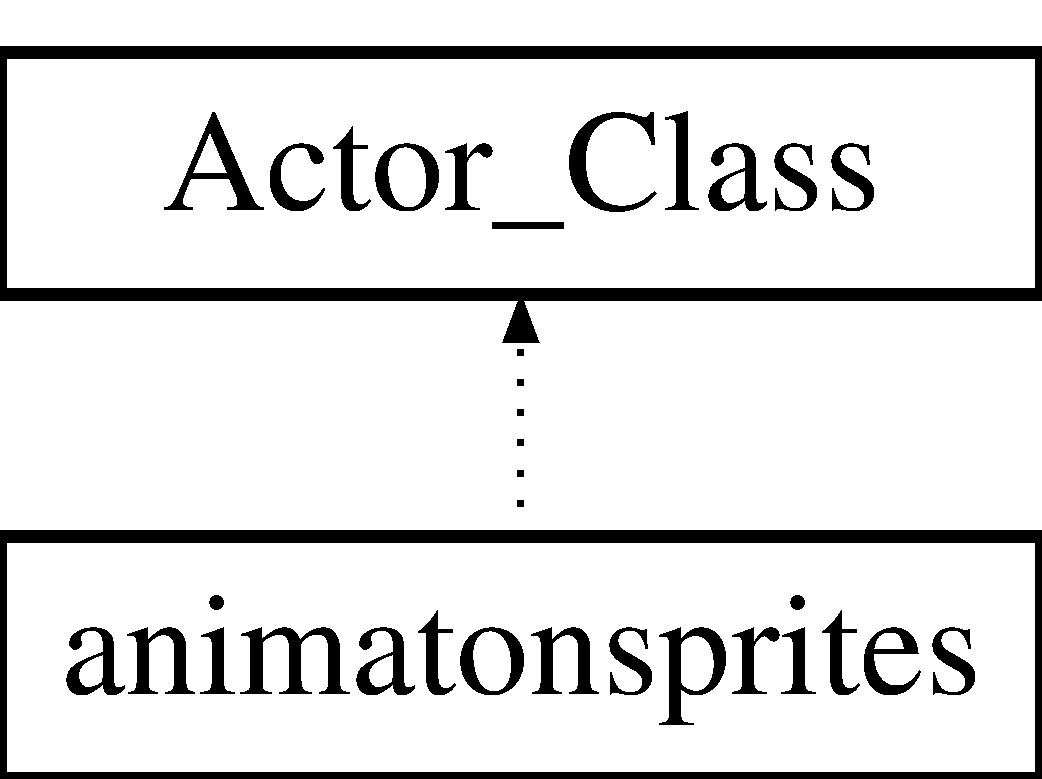
\includegraphics[height=2.000000cm]{classanimatonsprites}
\end{center}
\end{figure}
\subsection*{Public Member Functions}
\begin{DoxyCompactItemize}
\item 
\hyperlink{classanimatonsprites_a68866689ab26f4a7fff5d3d44a8c46b9}{animatonsprites} ()
\item 
void \hyperlink{classanimatonsprites_a8f2c1a1d40776af39e45c125367fbc54}{animation\+Hero} (\hyperlink{class_actor___class}{Actor\+\_\+\+Class} $\ast$actor)
\item 
void \hyperlink{classanimatonsprites_aeef3560c6b0faaeb00af4a2b88a9ce5d}{animation\+Bullet} (\hyperlink{class_actor___class}{Actor\+\_\+\+Class} $\ast$actor)
\item 
void \hyperlink{classanimatonsprites_abd2ff02cecde1c8fa445c9c61dadb7b2}{Flying\+Boss} (\hyperlink{class_actor___class}{Actor\+\_\+\+Class} $\ast$actor)
\item 
void \hyperlink{classanimatonsprites_a82db8f9361e43e23f8044b35739dbb4f}{Turretanimation} (\hyperlink{class_actor___class}{Actor\+\_\+\+Class} $\ast$actor)
\item 
void \hyperlink{classanimatonsprites_a94dceae0ec3b4efe4940c4e8208ce1e6}{Dooranimation} (\hyperlink{class_actor___class}{Actor\+\_\+\+Class} $\ast$actor)
\item 
void \hyperlink{classanimatonsprites_a48b0fe9fa65a843657f026a1f56eedd8}{Bossanimtion} (\hyperlink{class_actor___class}{Actor\+\_\+\+Class} $\ast$actor)
\item 
void \hyperlink{classanimatonsprites_a45b6be4805c6e25497956b88c176f552}{jump} ()
\item 
void \hyperlink{classanimatonsprites_a1cf7f2fb8b5a3299b05052c8b6328f01}{move} ()
\item 
void \hyperlink{classanimatonsprites_ac009e9d25649abc90551981421de9f72}{draw} ()
\item 
void \hyperlink{classanimatonsprites_a50c1ab6bdeb5462156197f1208d8bde5}{death} ()
\end{DoxyCompactItemize}


\subsection{Detailed Description}


Definition at line 14 of file animatonsprites.\+h.



\subsection{Constructor \& Destructor Documentation}
\hypertarget{classanimatonsprites_a68866689ab26f4a7fff5d3d44a8c46b9}{}\label{classanimatonsprites_a68866689ab26f4a7fff5d3d44a8c46b9} 
\index{animatonsprites@{animatonsprites}!animatonsprites@{animatonsprites}}
\index{animatonsprites@{animatonsprites}!animatonsprites@{animatonsprites}}
\subsubsection{\texorpdfstring{animatonsprites()}{animatonsprites()}}
{\footnotesize\ttfamily animatonsprites\+::animatonsprites (\begin{DoxyParamCaption}{ }\end{DoxyParamCaption})\hspace{0.3cm}{\ttfamily [inline]}}



Definition at line 16 of file animatonsprites.\+h.



\subsection{Member Function Documentation}
\hypertarget{classanimatonsprites_aeef3560c6b0faaeb00af4a2b88a9ce5d}{}\label{classanimatonsprites_aeef3560c6b0faaeb00af4a2b88a9ce5d} 
\index{animatonsprites@{animatonsprites}!animation\+Bullet@{animation\+Bullet}}
\index{animation\+Bullet@{animation\+Bullet}!animatonsprites@{animatonsprites}}
\subsubsection{\texorpdfstring{animation\+Bullet()}{animationBullet()}}
{\footnotesize\ttfamily void animatonsprites\+::animation\+Bullet (\begin{DoxyParamCaption}\item[{\hyperlink{class_actor___class}{Actor\+\_\+\+Class} $\ast$}]{actor }\end{DoxyParamCaption})}



Definition at line 185 of file animatonsprites.\+cpp.

\hypertarget{classanimatonsprites_a8f2c1a1d40776af39e45c125367fbc54}{}\label{classanimatonsprites_a8f2c1a1d40776af39e45c125367fbc54} 
\index{animatonsprites@{animatonsprites}!animation\+Hero@{animation\+Hero}}
\index{animation\+Hero@{animation\+Hero}!animatonsprites@{animatonsprites}}
\subsubsection{\texorpdfstring{animation\+Hero()}{animationHero()}}
{\footnotesize\ttfamily void animatonsprites\+::animation\+Hero (\begin{DoxyParamCaption}\item[{\hyperlink{class_actor___class}{Actor\+\_\+\+Class} $\ast$}]{actor }\end{DoxyParamCaption})}



Definition at line 9 of file animatonsprites.\+cpp.

\hypertarget{classanimatonsprites_a48b0fe9fa65a843657f026a1f56eedd8}{}\label{classanimatonsprites_a48b0fe9fa65a843657f026a1f56eedd8} 
\index{animatonsprites@{animatonsprites}!Bossanimtion@{Bossanimtion}}
\index{Bossanimtion@{Bossanimtion}!animatonsprites@{animatonsprites}}
\subsubsection{\texorpdfstring{Bossanimtion()}{Bossanimtion()}}
{\footnotesize\ttfamily void animatonsprites\+::\+Bossanimtion (\begin{DoxyParamCaption}\item[{\hyperlink{class_actor___class}{Actor\+\_\+\+Class} $\ast$}]{actor }\end{DoxyParamCaption})}

\hypertarget{classanimatonsprites_a50c1ab6bdeb5462156197f1208d8bde5}{}\label{classanimatonsprites_a50c1ab6bdeb5462156197f1208d8bde5} 
\index{animatonsprites@{animatonsprites}!death@{death}}
\index{death@{death}!animatonsprites@{animatonsprites}}
\subsubsection{\texorpdfstring{death()}{death()}}
{\footnotesize\ttfamily void animatonsprites\+::death (\begin{DoxyParamCaption}{ }\end{DoxyParamCaption})\hspace{0.3cm}{\ttfamily [inline]}, {\ttfamily [virtual]}}



Reimplemented from \hyperlink{class_actor___class_a9447c6154a674d7e6bdf24ff2874b7a8}{Actor\+\_\+\+Class}.



Definition at line 28 of file animatonsprites.\+h.

\hypertarget{classanimatonsprites_a94dceae0ec3b4efe4940c4e8208ce1e6}{}\label{classanimatonsprites_a94dceae0ec3b4efe4940c4e8208ce1e6} 
\index{animatonsprites@{animatonsprites}!Dooranimation@{Dooranimation}}
\index{Dooranimation@{Dooranimation}!animatonsprites@{animatonsprites}}
\subsubsection{\texorpdfstring{Dooranimation()}{Dooranimation()}}
{\footnotesize\ttfamily void animatonsprites\+::\+Dooranimation (\begin{DoxyParamCaption}\item[{\hyperlink{class_actor___class}{Actor\+\_\+\+Class} $\ast$}]{actor }\end{DoxyParamCaption})}



Definition at line 385 of file animatonsprites.\+cpp.

\hypertarget{classanimatonsprites_ac009e9d25649abc90551981421de9f72}{}\label{classanimatonsprites_ac009e9d25649abc90551981421de9f72} 
\index{animatonsprites@{animatonsprites}!draw@{draw}}
\index{draw@{draw}!animatonsprites@{animatonsprites}}
\subsubsection{\texorpdfstring{draw()}{draw()}}
{\footnotesize\ttfamily void animatonsprites\+::draw (\begin{DoxyParamCaption}{ }\end{DoxyParamCaption})\hspace{0.3cm}{\ttfamily [inline]}, {\ttfamily [virtual]}}



Reimplemented from \hyperlink{class_actor___class_ac49cd62be76b4b950ecbe155413f1b64}{Actor\+\_\+\+Class}.



Definition at line 27 of file animatonsprites.\+h.

\hypertarget{classanimatonsprites_abd2ff02cecde1c8fa445c9c61dadb7b2}{}\label{classanimatonsprites_abd2ff02cecde1c8fa445c9c61dadb7b2} 
\index{animatonsprites@{animatonsprites}!Flying\+Boss@{Flying\+Boss}}
\index{Flying\+Boss@{Flying\+Boss}!animatonsprites@{animatonsprites}}
\subsubsection{\texorpdfstring{Flying\+Boss()}{FlyingBoss()}}
{\footnotesize\ttfamily void animatonsprites\+::\+Flying\+Boss (\begin{DoxyParamCaption}\item[{\hyperlink{class_actor___class}{Actor\+\_\+\+Class} $\ast$}]{actor }\end{DoxyParamCaption})}



Definition at line 323 of file animatonsprites.\+cpp.

\hypertarget{classanimatonsprites_a45b6be4805c6e25497956b88c176f552}{}\label{classanimatonsprites_a45b6be4805c6e25497956b88c176f552} 
\index{animatonsprites@{animatonsprites}!jump@{jump}}
\index{jump@{jump}!animatonsprites@{animatonsprites}}
\subsubsection{\texorpdfstring{jump()}{jump()}}
{\footnotesize\ttfamily void animatonsprites\+::jump (\begin{DoxyParamCaption}{ }\end{DoxyParamCaption})\hspace{0.3cm}{\ttfamily [inline]}, {\ttfamily [virtual]}}



Reimplemented from \hyperlink{class_actor___class_ab33216a3ce0c856bdc16231c71ae35c2}{Actor\+\_\+\+Class}.



Definition at line 25 of file animatonsprites.\+h.

\hypertarget{classanimatonsprites_a1cf7f2fb8b5a3299b05052c8b6328f01}{}\label{classanimatonsprites_a1cf7f2fb8b5a3299b05052c8b6328f01} 
\index{animatonsprites@{animatonsprites}!move@{move}}
\index{move@{move}!animatonsprites@{animatonsprites}}
\subsubsection{\texorpdfstring{move()}{move()}}
{\footnotesize\ttfamily void animatonsprites\+::move (\begin{DoxyParamCaption}{ }\end{DoxyParamCaption})\hspace{0.3cm}{\ttfamily [inline]}, {\ttfamily [virtual]}}



Reimplemented from \hyperlink{class_actor___class_af1764a94c5410ba8476f56553cd2c327}{Actor\+\_\+\+Class}.



Definition at line 26 of file animatonsprites.\+h.

\hypertarget{classanimatonsprites_a82db8f9361e43e23f8044b35739dbb4f}{}\label{classanimatonsprites_a82db8f9361e43e23f8044b35739dbb4f} 
\index{animatonsprites@{animatonsprites}!Turretanimation@{Turretanimation}}
\index{Turretanimation@{Turretanimation}!animatonsprites@{animatonsprites}}
\subsubsection{\texorpdfstring{Turretanimation()}{Turretanimation()}}
{\footnotesize\ttfamily void animatonsprites\+::\+Turretanimation (\begin{DoxyParamCaption}\item[{\hyperlink{class_actor___class}{Actor\+\_\+\+Class} $\ast$}]{actor }\end{DoxyParamCaption})}



Definition at line 359 of file animatonsprites.\+cpp.



The documentation for this class was generated from the following files\+:\begin{DoxyCompactItemize}
\item 
Actor/\hyperlink{animatonsprites_8h}{animatonsprites.\+h}\item 
Actor/\hyperlink{animatonsprites_8cpp}{animatonsprites.\+cpp}\end{DoxyCompactItemize}

\hypertarget{class_boss__door}{}\section{Boss\+\_\+door Class Reference}
\label{class_boss__door}\index{Boss\+\_\+door@{Boss\+\_\+door}}


{\ttfamily \#include $<$Boss\+\_\+door.\+h$>$}

Inheritance diagram for Boss\+\_\+door\+:\begin{figure}[H]
\begin{center}
\leavevmode
\includegraphics[height=3.000000cm]{class_boss__door}
\end{center}
\end{figure}
\subsection*{Public Member Functions}
\begin{DoxyCompactItemize}
\item 
\hyperlink{class_boss__door_a9714a08a688e8dc4819db1ade1d502fd}{Boss\+\_\+door} (sf\+::\+Render\+Window \&window, \hyperlink{class_collision}{Collision} \hyperlink{class_boss__door_a591dd5dd3815c47b2f8390fe63953ac2}{col}, int x\+Inn, int y\+Inn)
\item 
void \hyperlink{class_boss__door_ac2f0b88b5ca332380602f029f0f83e17}{jump} ()
\item 
void \hyperlink{class_boss__door_a27456c378555a03310cd4f25b167867c}{move} ()
\item 
void \hyperlink{class_boss__door_a093ca3c013ae4f5f703675bc6d3de9f0}{draw} ()
\item 
void \hyperlink{class_boss__door_ab80f398f1c479f78c2b36409c311ccb5}{interaction} (std\+::vector$<$ \hyperlink{class_actor___class}{Actor\+\_\+\+Class} $\ast$$>$ actor\+\_\+array)
\item 
void \hyperlink{class_boss__door_ab47df13fb29b88a5be09fb7062384a50}{interaction\+\_\+effect} (\hyperlink{class_actor___class}{Actor\+\_\+\+Class} $\ast$actor)
\item 
void \hyperlink{class_boss__door_acee93d541699ed109dfae8f05f0ea39e}{death} ()
\end{DoxyCompactItemize}
\subsection*{Public Attributes}
\begin{DoxyCompactItemize}
\item 
sf\+::\+Rectangle\+Shape \hyperlink{class_boss__door_a8b719291e134d7cf4bee8fd2372d3087}{door}
\item 
\hyperlink{classanimatonsprites}{animatonsprites} \hyperlink{class_boss__door_a78f03723848d84a1eae62fafa7933f92}{animation}
\item 
sf\+::\+Render\+Window \& \hyperlink{class_boss__door_a41a5f7ad972a57cc11fa7629d4cce412}{vindu}
\item 
\hyperlink{class_collision}{Collision} \hyperlink{class_boss__door_a591dd5dd3815c47b2f8390fe63953ac2}{col}
\item 
float \hyperlink{class_boss__door_a780a847f966efcd3073642ade6a7c97f}{gravity} = 5
\item 
int \hyperlink{class_boss__door_aa9c098587ea1c0919540f838e28c1440}{startX} =400
\begin{DoxyCompactList}\small\item\em float floor =400;//bør byttes ut med at det er localisasjonen den intersecter med en title \end{DoxyCompactList}\item 
int \hyperlink{class_boss__door_a617e52e98386b7202fc78a24c4f5037d}{startY} =20
\end{DoxyCompactItemize}
\subsection*{Additional Inherited Members}


\subsection{Detailed Description}


Definition at line 15 of file Boss\+\_\+door.\+h.



\subsection{Constructor \& Destructor Documentation}
\hypertarget{class_boss__door_a9714a08a688e8dc4819db1ade1d502fd}{}\label{class_boss__door_a9714a08a688e8dc4819db1ade1d502fd} 
\index{Boss\+\_\+door@{Boss\+\_\+door}!Boss\+\_\+door@{Boss\+\_\+door}}
\index{Boss\+\_\+door@{Boss\+\_\+door}!Boss\+\_\+door@{Boss\+\_\+door}}
\subsubsection{\texorpdfstring{Boss\+\_\+door()}{Boss\_door()}}
{\footnotesize\ttfamily Boss\+\_\+door\+::\+Boss\+\_\+door (\begin{DoxyParamCaption}\item[{sf\+::\+Render\+Window \&}]{window,  }\item[{\hyperlink{class_collision}{Collision}}]{col,  }\item[{int}]{x\+Inn,  }\item[{int}]{y\+Inn }\end{DoxyParamCaption})}



Definition at line 6 of file Boss\+\_\+door.\+cpp.



\subsection{Member Function Documentation}
\hypertarget{class_boss__door_acee93d541699ed109dfae8f05f0ea39e}{}\label{class_boss__door_acee93d541699ed109dfae8f05f0ea39e} 
\index{Boss\+\_\+door@{Boss\+\_\+door}!death@{death}}
\index{death@{death}!Boss\+\_\+door@{Boss\+\_\+door}}
\subsubsection{\texorpdfstring{death()}{death()}}
{\footnotesize\ttfamily void Boss\+\_\+door\+::death (\begin{DoxyParamCaption}{ }\end{DoxyParamCaption})\hspace{0.3cm}{\ttfamily [virtual]}}



Reimplemented from \hyperlink{class_actor___class_a9447c6154a674d7e6bdf24ff2874b7a8}{Actor\+\_\+\+Class}.



Definition at line 92 of file Boss\+\_\+door.\+cpp.

\hypertarget{class_boss__door_a093ca3c013ae4f5f703675bc6d3de9f0}{}\label{class_boss__door_a093ca3c013ae4f5f703675bc6d3de9f0} 
\index{Boss\+\_\+door@{Boss\+\_\+door}!draw@{draw}}
\index{draw@{draw}!Boss\+\_\+door@{Boss\+\_\+door}}
\subsubsection{\texorpdfstring{draw()}{draw()}}
{\footnotesize\ttfamily void Boss\+\_\+door\+::draw (\begin{DoxyParamCaption}{ }\end{DoxyParamCaption})\hspace{0.3cm}{\ttfamily [virtual]}}



Reimplemented from \hyperlink{class_actor___class_ac49cd62be76b4b950ecbe155413f1b64}{Actor\+\_\+\+Class}.



Definition at line 36 of file Boss\+\_\+door.\+cpp.

\hypertarget{class_boss__door_ab80f398f1c479f78c2b36409c311ccb5}{}\label{class_boss__door_ab80f398f1c479f78c2b36409c311ccb5} 
\index{Boss\+\_\+door@{Boss\+\_\+door}!interaction@{interaction}}
\index{interaction@{interaction}!Boss\+\_\+door@{Boss\+\_\+door}}
\subsubsection{\texorpdfstring{interaction()}{interaction()}}
{\footnotesize\ttfamily void Boss\+\_\+door\+::interaction (\begin{DoxyParamCaption}\item[{std\+::vector$<$ \hyperlink{class_actor___class}{Actor\+\_\+\+Class} $\ast$$>$}]{actor\+\_\+array }\end{DoxyParamCaption})\hspace{0.3cm}{\ttfamily [virtual]}}



Reimplemented from \hyperlink{class_actor___class_a87d1e079d8576fa99592a60b38a04a1b}{Actor\+\_\+\+Class}.



Definition at line 50 of file Boss\+\_\+door.\+cpp.

\hypertarget{class_boss__door_ab47df13fb29b88a5be09fb7062384a50}{}\label{class_boss__door_ab47df13fb29b88a5be09fb7062384a50} 
\index{Boss\+\_\+door@{Boss\+\_\+door}!interaction\+\_\+effect@{interaction\+\_\+effect}}
\index{interaction\+\_\+effect@{interaction\+\_\+effect}!Boss\+\_\+door@{Boss\+\_\+door}}
\subsubsection{\texorpdfstring{interaction\+\_\+effect()}{interaction\_effect()}}
{\footnotesize\ttfamily void Boss\+\_\+door\+::interaction\+\_\+effect (\begin{DoxyParamCaption}\item[{\hyperlink{class_actor___class}{Actor\+\_\+\+Class} $\ast$}]{actor }\end{DoxyParamCaption})\hspace{0.3cm}{\ttfamily [virtual]}}



Reimplemented from \hyperlink{class_actor___class_af3488ca470eb77255060142fd167aa72}{Actor\+\_\+\+Class}.



Definition at line 75 of file Boss\+\_\+door.\+cpp.

\hypertarget{class_boss__door_ac2f0b88b5ca332380602f029f0f83e17}{}\label{class_boss__door_ac2f0b88b5ca332380602f029f0f83e17} 
\index{Boss\+\_\+door@{Boss\+\_\+door}!jump@{jump}}
\index{jump@{jump}!Boss\+\_\+door@{Boss\+\_\+door}}
\subsubsection{\texorpdfstring{jump()}{jump()}}
{\footnotesize\ttfamily void Boss\+\_\+door\+::jump (\begin{DoxyParamCaption}{ }\end{DoxyParamCaption})\hspace{0.3cm}{\ttfamily [virtual]}}



Reimplemented from \hyperlink{class_actor___class_ab33216a3ce0c856bdc16231c71ae35c2}{Actor\+\_\+\+Class}.



Definition at line 46 of file Boss\+\_\+door.\+cpp.

\hypertarget{class_boss__door_a27456c378555a03310cd4f25b167867c}{}\label{class_boss__door_a27456c378555a03310cd4f25b167867c} 
\index{Boss\+\_\+door@{Boss\+\_\+door}!move@{move}}
\index{move@{move}!Boss\+\_\+door@{Boss\+\_\+door}}
\subsubsection{\texorpdfstring{move()}{move()}}
{\footnotesize\ttfamily void Boss\+\_\+door\+::move (\begin{DoxyParamCaption}{ }\end{DoxyParamCaption})\hspace{0.3cm}{\ttfamily [virtual]}}



Reimplemented from \hyperlink{class_actor___class_af1764a94c5410ba8476f56553cd2c327}{Actor\+\_\+\+Class}.



Definition at line 31 of file Boss\+\_\+door.\+cpp.



\subsection{Member Data Documentation}
\hypertarget{class_boss__door_a78f03723848d84a1eae62fafa7933f92}{}\label{class_boss__door_a78f03723848d84a1eae62fafa7933f92} 
\index{Boss\+\_\+door@{Boss\+\_\+door}!animation@{animation}}
\index{animation@{animation}!Boss\+\_\+door@{Boss\+\_\+door}}
\subsubsection{\texorpdfstring{animation}{animation}}
{\footnotesize\ttfamily \hyperlink{classanimatonsprites}{animatonsprites} Boss\+\_\+door\+::animation}



Definition at line 21 of file Boss\+\_\+door.\+h.

\hypertarget{class_boss__door_a591dd5dd3815c47b2f8390fe63953ac2}{}\label{class_boss__door_a591dd5dd3815c47b2f8390fe63953ac2} 
\index{Boss\+\_\+door@{Boss\+\_\+door}!col@{col}}
\index{col@{col}!Boss\+\_\+door@{Boss\+\_\+door}}
\subsubsection{\texorpdfstring{col}{col}}
{\footnotesize\ttfamily \hyperlink{class_collision}{Collision} Boss\+\_\+door\+::col}



Definition at line 24 of file Boss\+\_\+door.\+h.

\hypertarget{class_boss__door_a8b719291e134d7cf4bee8fd2372d3087}{}\label{class_boss__door_a8b719291e134d7cf4bee8fd2372d3087} 
\index{Boss\+\_\+door@{Boss\+\_\+door}!door@{door}}
\index{door@{door}!Boss\+\_\+door@{Boss\+\_\+door}}
\subsubsection{\texorpdfstring{door}{door}}
{\footnotesize\ttfamily sf\+::\+Rectangle\+Shape Boss\+\_\+door\+::door}



Definition at line 20 of file Boss\+\_\+door.\+h.

\hypertarget{class_boss__door_a780a847f966efcd3073642ade6a7c97f}{}\label{class_boss__door_a780a847f966efcd3073642ade6a7c97f} 
\index{Boss\+\_\+door@{Boss\+\_\+door}!gravity@{gravity}}
\index{gravity@{gravity}!Boss\+\_\+door@{Boss\+\_\+door}}
\subsubsection{\texorpdfstring{gravity}{gravity}}
{\footnotesize\ttfamily float Boss\+\_\+door\+::gravity = 5}



Definition at line 26 of file Boss\+\_\+door.\+h.

\hypertarget{class_boss__door_aa9c098587ea1c0919540f838e28c1440}{}\label{class_boss__door_aa9c098587ea1c0919540f838e28c1440} 
\index{Boss\+\_\+door@{Boss\+\_\+door}!startX@{startX}}
\index{startX@{startX}!Boss\+\_\+door@{Boss\+\_\+door}}
\subsubsection{\texorpdfstring{startX}{startX}}
{\footnotesize\ttfamily int Boss\+\_\+door\+::startX =400}



float floor =400;//bør byttes ut med at det er localisasjonen den intersecter med en title 



Definition at line 32 of file Boss\+\_\+door.\+h.

\hypertarget{class_boss__door_a617e52e98386b7202fc78a24c4f5037d}{}\label{class_boss__door_a617e52e98386b7202fc78a24c4f5037d} 
\index{Boss\+\_\+door@{Boss\+\_\+door}!startY@{startY}}
\index{startY@{startY}!Boss\+\_\+door@{Boss\+\_\+door}}
\subsubsection{\texorpdfstring{startY}{startY}}
{\footnotesize\ttfamily int Boss\+\_\+door\+::startY =20}



Definition at line 33 of file Boss\+\_\+door.\+h.

\hypertarget{class_boss__door_a41a5f7ad972a57cc11fa7629d4cce412}{}\label{class_boss__door_a41a5f7ad972a57cc11fa7629d4cce412} 
\index{Boss\+\_\+door@{Boss\+\_\+door}!vindu@{vindu}}
\index{vindu@{vindu}!Boss\+\_\+door@{Boss\+\_\+door}}
\subsubsection{\texorpdfstring{vindu}{vindu}}
{\footnotesize\ttfamily sf\+::\+Render\+Window\& Boss\+\_\+door\+::vindu}



Definition at line 23 of file Boss\+\_\+door.\+h.



The documentation for this class was generated from the following files\+:\begin{DoxyCompactItemize}
\item 
Actor/enemy/\hyperlink{_boss__door_8h}{Boss\+\_\+door.\+h}\item 
Actor/enemy/\hyperlink{_boss__door_8cpp}{Boss\+\_\+door.\+cpp}\end{DoxyCompactItemize}

\hypertarget{classboss__enemy__2}{}\section{boss\+\_\+enemy\+\_\+2 Class Reference}
\label{classboss__enemy__2}\index{boss\+\_\+enemy\+\_\+2@{boss\+\_\+enemy\+\_\+2}}


{\ttfamily \#include $<$boss\+\_\+enemy\+\_\+2.\+h$>$}

Inheritance diagram for boss\+\_\+enemy\+\_\+2\+:\begin{figure}[H]
\begin{center}
\leavevmode
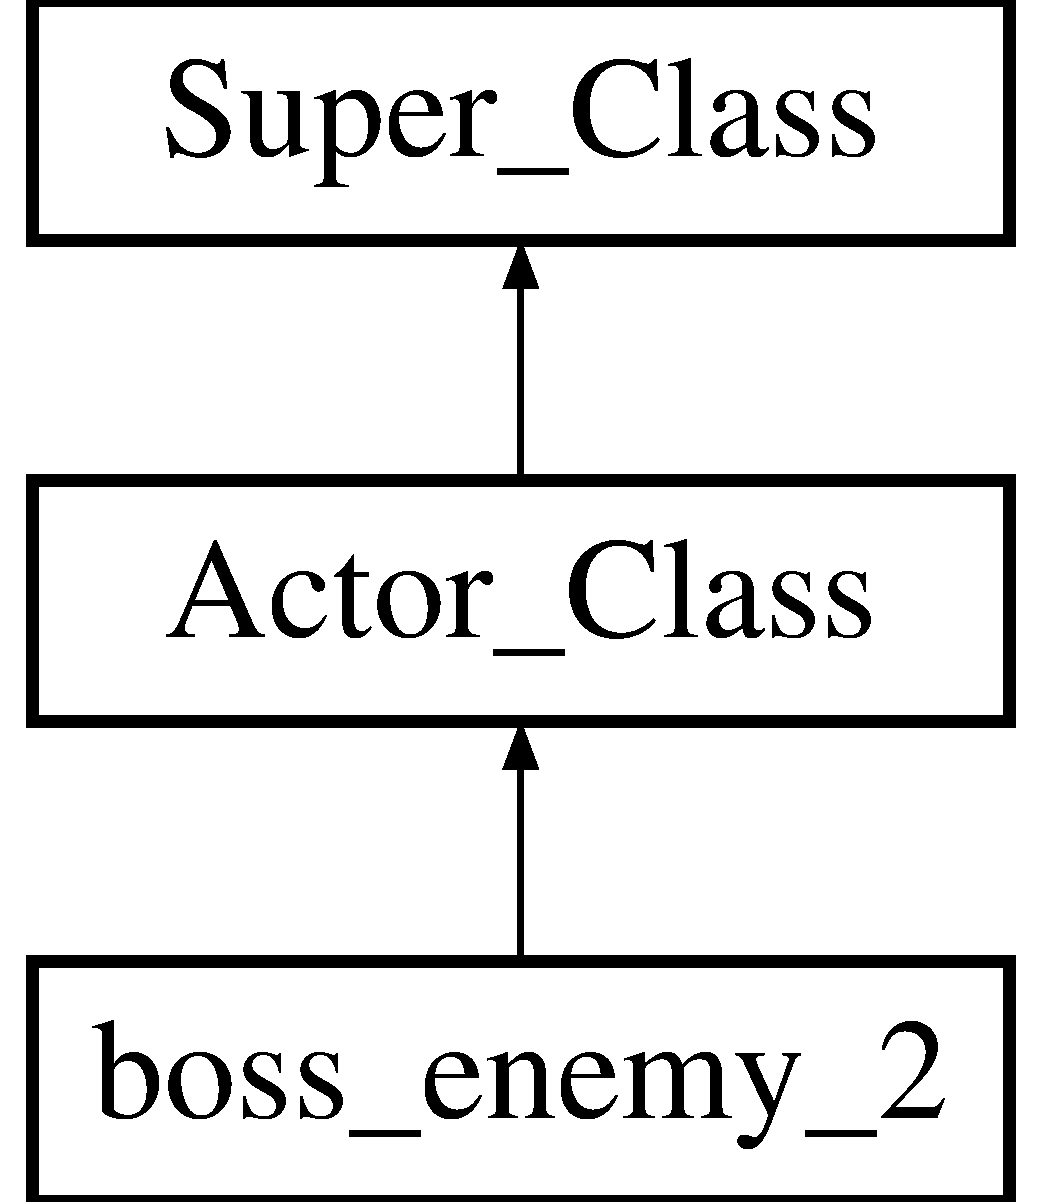
\includegraphics[height=3.000000cm]{classboss__enemy__2}
\end{center}
\end{figure}
\subsection*{Public Member Functions}
\begin{DoxyCompactItemize}
\item 
\hyperlink{classboss__enemy__2_a5090ddbdea5fedbd070705079b053c14}{boss\+\_\+enemy\+\_\+2} (sf\+::\+Render\+Window \&window, \hyperlink{class_collision}{Collision} \hyperlink{classboss__enemy__2_a59f86459a90bbd1ad535889e9197cb6f}{col}, int x\+Inn, int y\+Inn)
\item 
void \hyperlink{classboss__enemy__2_a7edccc066047aacf21797b6d4316f57c}{jump} ()
\item 
void \hyperlink{classboss__enemy__2_a8d81c7498b4a31d735bd4af21ce81d84}{move} ()
\item 
void \hyperlink{classboss__enemy__2_aea8e734cf65b63f1d8ba143f3b449f63}{draw} ()
\item 
void \hyperlink{classboss__enemy__2_a6315561045c1530e588014caaf6a9292}{action} ()
\item 
void \hyperlink{classboss__enemy__2_a602bdac1d534a3d37e9cd76616216b45}{death} ()
\end{DoxyCompactItemize}
\subsection*{Public Attributes}
\begin{DoxyCompactItemize}
\item 
sf\+::\+Music \hyperlink{classboss__enemy__2_a46f313cdeff7cbfe637e3b4f6600cc68}{sound}
\item 
sf\+::\+Rectangle\+Shape \hyperlink{classboss__enemy__2_a1ffee874c7083f8bcdb2b66bef56daa2}{boss}
\item 
sf\+::\+Render\+Window \& \hyperlink{classboss__enemy__2_a009ce9fc4bc3da63a2380221f38df441}{vindu}
\item 
\hyperlink{class_collision}{Collision} \hyperlink{classboss__enemy__2_a59f86459a90bbd1ad535889e9197cb6f}{col}
\item 
float \hyperlink{classboss__enemy__2_a8abff95ac6b01b5d6b38f93f1c4060f7}{gravity} = 5
\item 
int \hyperlink{classboss__enemy__2_aabc3601b0121203650e78430aab3b309}{startX} =400
\begin{DoxyCompactList}\small\item\em float floor =400;//bør byttes ut med at det er localisasjonen den intersecter med en title \end{DoxyCompactList}\item 
int \hyperlink{classboss__enemy__2_a6e3d39e8276440d0b4b897aecc63839c}{startY} =20
\item 
int \hyperlink{classboss__enemy__2_a838ab901aab6f1e202d924dfc32dc420}{boss\+\_\+jump} = 50
\item 
int \hyperlink{classboss__enemy__2_ad07f609155076e0ee1fd0dcb015e05d0}{boss\+\_\+shoot} = 5
\item 
int \hyperlink{classboss__enemy__2_acda97e45d43d96c23c03f7aedaf0d537}{movment} =30
\end{DoxyCompactItemize}
\subsection*{Additional Inherited Members}


\subsection{Detailed Description}


Definition at line 14 of file boss\+\_\+enemy\+\_\+2.\+h.



\subsection{Constructor \& Destructor Documentation}
\hypertarget{classboss__enemy__2_a5090ddbdea5fedbd070705079b053c14}{}\label{classboss__enemy__2_a5090ddbdea5fedbd070705079b053c14} 
\index{boss\+\_\+enemy\+\_\+2@{boss\+\_\+enemy\+\_\+2}!boss\+\_\+enemy\+\_\+2@{boss\+\_\+enemy\+\_\+2}}
\index{boss\+\_\+enemy\+\_\+2@{boss\+\_\+enemy\+\_\+2}!boss\+\_\+enemy\+\_\+2@{boss\+\_\+enemy\+\_\+2}}
\subsubsection{\texorpdfstring{boss\+\_\+enemy\+\_\+2()}{boss\_enemy\_2()}}
{\footnotesize\ttfamily boss\+\_\+enemy\+\_\+2\+::boss\+\_\+enemy\+\_\+2 (\begin{DoxyParamCaption}\item[{sf\+::\+Render\+Window \&}]{window,  }\item[{\hyperlink{class_collision}{Collision}}]{col,  }\item[{int}]{x\+Inn,  }\item[{int}]{y\+Inn }\end{DoxyParamCaption})}

ensures that the hero texture has been loaded 

Definition at line 8 of file boss\+\_\+enemy\+\_\+2.\+cpp.



\subsection{Member Function Documentation}
\hypertarget{classboss__enemy__2_a6315561045c1530e588014caaf6a9292}{}\label{classboss__enemy__2_a6315561045c1530e588014caaf6a9292} 
\index{boss\+\_\+enemy\+\_\+2@{boss\+\_\+enemy\+\_\+2}!action@{action}}
\index{action@{action}!boss\+\_\+enemy\+\_\+2@{boss\+\_\+enemy\+\_\+2}}
\subsubsection{\texorpdfstring{action()}{action()}}
{\footnotesize\ttfamily void boss\+\_\+enemy\+\_\+2\+::action (\begin{DoxyParamCaption}{ }\end{DoxyParamCaption})\hspace{0.3cm}{\ttfamily [virtual]}}



Reimplemented from \hyperlink{class_actor___class_ab8e23ffae108da3b8eda67c6753bdae0}{Actor\+\_\+\+Class}.



Definition at line 111 of file boss\+\_\+enemy\+\_\+2.\+cpp.

\hypertarget{classboss__enemy__2_a602bdac1d534a3d37e9cd76616216b45}{}\label{classboss__enemy__2_a602bdac1d534a3d37e9cd76616216b45} 
\index{boss\+\_\+enemy\+\_\+2@{boss\+\_\+enemy\+\_\+2}!death@{death}}
\index{death@{death}!boss\+\_\+enemy\+\_\+2@{boss\+\_\+enemy\+\_\+2}}
\subsubsection{\texorpdfstring{death()}{death()}}
{\footnotesize\ttfamily void boss\+\_\+enemy\+\_\+2\+::death (\begin{DoxyParamCaption}{ }\end{DoxyParamCaption})\hspace{0.3cm}{\ttfamily [virtual]}}



Reimplemented from \hyperlink{class_actor___class_a9447c6154a674d7e6bdf24ff2874b7a8}{Actor\+\_\+\+Class}.



Definition at line 123 of file boss\+\_\+enemy\+\_\+2.\+cpp.

\hypertarget{classboss__enemy__2_aea8e734cf65b63f1d8ba143f3b449f63}{}\label{classboss__enemy__2_aea8e734cf65b63f1d8ba143f3b449f63} 
\index{boss\+\_\+enemy\+\_\+2@{boss\+\_\+enemy\+\_\+2}!draw@{draw}}
\index{draw@{draw}!boss\+\_\+enemy\+\_\+2@{boss\+\_\+enemy\+\_\+2}}
\subsubsection{\texorpdfstring{draw()}{draw()}}
{\footnotesize\ttfamily void boss\+\_\+enemy\+\_\+2\+::draw (\begin{DoxyParamCaption}{ }\end{DoxyParamCaption})\hspace{0.3cm}{\ttfamily [virtual]}}



Reimplemented from \hyperlink{class_actor___class_ac49cd62be76b4b950ecbe155413f1b64}{Actor\+\_\+\+Class}.



Definition at line 139 of file boss\+\_\+enemy\+\_\+2.\+cpp.

\hypertarget{classboss__enemy__2_a7edccc066047aacf21797b6d4316f57c}{}\label{classboss__enemy__2_a7edccc066047aacf21797b6d4316f57c} 
\index{boss\+\_\+enemy\+\_\+2@{boss\+\_\+enemy\+\_\+2}!jump@{jump}}
\index{jump@{jump}!boss\+\_\+enemy\+\_\+2@{boss\+\_\+enemy\+\_\+2}}
\subsubsection{\texorpdfstring{jump()}{jump()}}
{\footnotesize\ttfamily void boss\+\_\+enemy\+\_\+2\+::jump (\begin{DoxyParamCaption}{ }\end{DoxyParamCaption})\hspace{0.3cm}{\ttfamily [virtual]}}



Reimplemented from \hyperlink{class_actor___class_ab33216a3ce0c856bdc16231c71ae35c2}{Actor\+\_\+\+Class}.



Definition at line 90 of file boss\+\_\+enemy\+\_\+2.\+cpp.

\hypertarget{classboss__enemy__2_a8d81c7498b4a31d735bd4af21ce81d84}{}\label{classboss__enemy__2_a8d81c7498b4a31d735bd4af21ce81d84} 
\index{boss\+\_\+enemy\+\_\+2@{boss\+\_\+enemy\+\_\+2}!move@{move}}
\index{move@{move}!boss\+\_\+enemy\+\_\+2@{boss\+\_\+enemy\+\_\+2}}
\subsubsection{\texorpdfstring{move()}{move()}}
{\footnotesize\ttfamily void boss\+\_\+enemy\+\_\+2\+::move (\begin{DoxyParamCaption}{ }\end{DoxyParamCaption})\hspace{0.3cm}{\ttfamily [virtual]}}



Reimplemented from \hyperlink{class_actor___class_af1764a94c5410ba8476f56553cd2c327}{Actor\+\_\+\+Class}.



Definition at line 49 of file boss\+\_\+enemy\+\_\+2.\+cpp.



\subsection{Member Data Documentation}
\hypertarget{classboss__enemy__2_a1ffee874c7083f8bcdb2b66bef56daa2}{}\label{classboss__enemy__2_a1ffee874c7083f8bcdb2b66bef56daa2} 
\index{boss\+\_\+enemy\+\_\+2@{boss\+\_\+enemy\+\_\+2}!boss@{boss}}
\index{boss@{boss}!boss\+\_\+enemy\+\_\+2@{boss\+\_\+enemy\+\_\+2}}
\subsubsection{\texorpdfstring{boss}{boss}}
{\footnotesize\ttfamily sf\+::\+Rectangle\+Shape boss\+\_\+enemy\+\_\+2\+::boss}



Definition at line 22 of file boss\+\_\+enemy\+\_\+2.\+h.

\hypertarget{classboss__enemy__2_a838ab901aab6f1e202d924dfc32dc420}{}\label{classboss__enemy__2_a838ab901aab6f1e202d924dfc32dc420} 
\index{boss\+\_\+enemy\+\_\+2@{boss\+\_\+enemy\+\_\+2}!boss\+\_\+jump@{boss\+\_\+jump}}
\index{boss\+\_\+jump@{boss\+\_\+jump}!boss\+\_\+enemy\+\_\+2@{boss\+\_\+enemy\+\_\+2}}
\subsubsection{\texorpdfstring{boss\+\_\+jump}{boss\_jump}}
{\footnotesize\ttfamily int boss\+\_\+enemy\+\_\+2\+::boss\+\_\+jump = 50}



Definition at line 35 of file boss\+\_\+enemy\+\_\+2.\+h.

\hypertarget{classboss__enemy__2_ad07f609155076e0ee1fd0dcb015e05d0}{}\label{classboss__enemy__2_ad07f609155076e0ee1fd0dcb015e05d0} 
\index{boss\+\_\+enemy\+\_\+2@{boss\+\_\+enemy\+\_\+2}!boss\+\_\+shoot@{boss\+\_\+shoot}}
\index{boss\+\_\+shoot@{boss\+\_\+shoot}!boss\+\_\+enemy\+\_\+2@{boss\+\_\+enemy\+\_\+2}}
\subsubsection{\texorpdfstring{boss\+\_\+shoot}{boss\_shoot}}
{\footnotesize\ttfamily int boss\+\_\+enemy\+\_\+2\+::boss\+\_\+shoot = 5}



Definition at line 36 of file boss\+\_\+enemy\+\_\+2.\+h.

\hypertarget{classboss__enemy__2_a59f86459a90bbd1ad535889e9197cb6f}{}\label{classboss__enemy__2_a59f86459a90bbd1ad535889e9197cb6f} 
\index{boss\+\_\+enemy\+\_\+2@{boss\+\_\+enemy\+\_\+2}!col@{col}}
\index{col@{col}!boss\+\_\+enemy\+\_\+2@{boss\+\_\+enemy\+\_\+2}}
\subsubsection{\texorpdfstring{col}{col}}
{\footnotesize\ttfamily \hyperlink{class_collision}{Collision} boss\+\_\+enemy\+\_\+2\+::col}



Definition at line 25 of file boss\+\_\+enemy\+\_\+2.\+h.

\hypertarget{classboss__enemy__2_a8abff95ac6b01b5d6b38f93f1c4060f7}{}\label{classboss__enemy__2_a8abff95ac6b01b5d6b38f93f1c4060f7} 
\index{boss\+\_\+enemy\+\_\+2@{boss\+\_\+enemy\+\_\+2}!gravity@{gravity}}
\index{gravity@{gravity}!boss\+\_\+enemy\+\_\+2@{boss\+\_\+enemy\+\_\+2}}
\subsubsection{\texorpdfstring{gravity}{gravity}}
{\footnotesize\ttfamily float boss\+\_\+enemy\+\_\+2\+::gravity = 5}



Definition at line 27 of file boss\+\_\+enemy\+\_\+2.\+h.

\hypertarget{classboss__enemy__2_acda97e45d43d96c23c03f7aedaf0d537}{}\label{classboss__enemy__2_acda97e45d43d96c23c03f7aedaf0d537} 
\index{boss\+\_\+enemy\+\_\+2@{boss\+\_\+enemy\+\_\+2}!movment@{movment}}
\index{movment@{movment}!boss\+\_\+enemy\+\_\+2@{boss\+\_\+enemy\+\_\+2}}
\subsubsection{\texorpdfstring{movment}{movment}}
{\footnotesize\ttfamily int boss\+\_\+enemy\+\_\+2\+::movment =30}



Definition at line 37 of file boss\+\_\+enemy\+\_\+2.\+h.

\hypertarget{classboss__enemy__2_a46f313cdeff7cbfe637e3b4f6600cc68}{}\label{classboss__enemy__2_a46f313cdeff7cbfe637e3b4f6600cc68} 
\index{boss\+\_\+enemy\+\_\+2@{boss\+\_\+enemy\+\_\+2}!sound@{sound}}
\index{sound@{sound}!boss\+\_\+enemy\+\_\+2@{boss\+\_\+enemy\+\_\+2}}
\subsubsection{\texorpdfstring{sound}{sound}}
{\footnotesize\ttfamily sf\+::\+Music boss\+\_\+enemy\+\_\+2\+::sound}



Definition at line 21 of file boss\+\_\+enemy\+\_\+2.\+h.

\hypertarget{classboss__enemy__2_aabc3601b0121203650e78430aab3b309}{}\label{classboss__enemy__2_aabc3601b0121203650e78430aab3b309} 
\index{boss\+\_\+enemy\+\_\+2@{boss\+\_\+enemy\+\_\+2}!startX@{startX}}
\index{startX@{startX}!boss\+\_\+enemy\+\_\+2@{boss\+\_\+enemy\+\_\+2}}
\subsubsection{\texorpdfstring{startX}{startX}}
{\footnotesize\ttfamily int boss\+\_\+enemy\+\_\+2\+::startX =400}



float floor =400;//bør byttes ut med at det er localisasjonen den intersecter med en title 



Definition at line 33 of file boss\+\_\+enemy\+\_\+2.\+h.

\hypertarget{classboss__enemy__2_a6e3d39e8276440d0b4b897aecc63839c}{}\label{classboss__enemy__2_a6e3d39e8276440d0b4b897aecc63839c} 
\index{boss\+\_\+enemy\+\_\+2@{boss\+\_\+enemy\+\_\+2}!startY@{startY}}
\index{startY@{startY}!boss\+\_\+enemy\+\_\+2@{boss\+\_\+enemy\+\_\+2}}
\subsubsection{\texorpdfstring{startY}{startY}}
{\footnotesize\ttfamily int boss\+\_\+enemy\+\_\+2\+::startY =20}



Definition at line 34 of file boss\+\_\+enemy\+\_\+2.\+h.

\hypertarget{classboss__enemy__2_a009ce9fc4bc3da63a2380221f38df441}{}\label{classboss__enemy__2_a009ce9fc4bc3da63a2380221f38df441} 
\index{boss\+\_\+enemy\+\_\+2@{boss\+\_\+enemy\+\_\+2}!vindu@{vindu}}
\index{vindu@{vindu}!boss\+\_\+enemy\+\_\+2@{boss\+\_\+enemy\+\_\+2}}
\subsubsection{\texorpdfstring{vindu}{vindu}}
{\footnotesize\ttfamily sf\+::\+Render\+Window\& boss\+\_\+enemy\+\_\+2\+::vindu}



Definition at line 24 of file boss\+\_\+enemy\+\_\+2.\+h.



The documentation for this class was generated from the following files\+:\begin{DoxyCompactItemize}
\item 
Actor/enemy/\hyperlink{boss__enemy__2_8h}{boss\+\_\+enemy\+\_\+2.\+h}\item 
Actor/enemy/\hyperlink{boss__enemy__2_8cpp}{boss\+\_\+enemy\+\_\+2.\+cpp}\end{DoxyCompactItemize}

\hypertarget{classboss__fight__1}{}\section{boss\+\_\+fight\+\_\+1 Class Reference}
\label{classboss__fight__1}\index{boss\+\_\+fight\+\_\+1@{boss\+\_\+fight\+\_\+1}}


{\ttfamily \#include $<$boss\+\_\+fight\+\_\+1.\+h$>$}

Inheritance diagram for boss\+\_\+fight\+\_\+1\+:\begin{figure}[H]
\begin{center}
\leavevmode
\includegraphics[height=3.000000cm]{classboss__fight__1}
\end{center}
\end{figure}
\subsection*{Public Member Functions}
\begin{DoxyCompactItemize}
\item 
\hyperlink{classboss__fight__1_a189fa85c3b23bb89776bebaa9f8dce70}{boss\+\_\+fight\+\_\+1} (sf\+::\+Render\+Window \&window, \hyperlink{class_collision}{Collision} \hyperlink{classboss__fight__1_a7419d00c4958618eaffb181617305d22}{col}, int x\+Inn, int y\+Inn)
\item 
void \hyperlink{classboss__fight__1_a363121fd16c5d41889f96405544bccc1}{jump} ()
\item 
void \hyperlink{classboss__fight__1_a2ecde11495757971f23f45e78f23c5f7}{move} ()
\item 
void \hyperlink{classboss__fight__1_a83b20e761e3f8781c8fee8d2be5442b0}{draw} ()
\item 
void \hyperlink{classboss__fight__1_a73c37c9ddf1b6370d1a9e2b5c9cd9b05}{action} ()
\item 
void \hyperlink{classboss__fight__1_a158e53600a084e13047732d89a0f4299}{death} ()
\end{DoxyCompactItemize}
\subsection*{Public Attributes}
\begin{DoxyCompactItemize}
\item 
sf\+::\+Music \hyperlink{classboss__fight__1_a7256c118906cf857f86beeb667291a91}{sound}
\item 
sf\+::\+Rectangle\+Shape \hyperlink{classboss__fight__1_a1bbb6010e2d4fce0052b99b66968e694}{boss}
\item 
sf\+::\+Render\+Window \& \hyperlink{classboss__fight__1_a87a27b1265ff58f25c6074405c93487e}{vindu}
\item 
\hyperlink{class_collision}{Collision} \hyperlink{classboss__fight__1_a7419d00c4958618eaffb181617305d22}{col}
\item 
float \hyperlink{classboss__fight__1_a4f0ada94e6586c2e825abaf789d9269d}{gravity} = 5
\item 
int \hyperlink{classboss__fight__1_af45fe739248b1b3da432ec4ab0770913}{startX} =400
\begin{DoxyCompactList}\small\item\em float floor =400;//bør byttes ut med at det er localisasjonen den intersecter med en title \end{DoxyCompactList}\item 
int \hyperlink{classboss__fight__1_a71884d8bccccd003e7b53acc6b86d513}{startY} =20
\item 
int \hyperlink{classboss__fight__1_ab020b6b32106cae5a2bdddef0443e5eb}{boss\+\_\+jump} = 50
\item 
int \hyperlink{classboss__fight__1_acdad682eac9821b3c2eb876eb1d99b90}{boss\+\_\+shoot} = 5
\end{DoxyCompactItemize}
\subsection*{Additional Inherited Members}


\subsection{Detailed Description}


Definition at line 14 of file boss\+\_\+fight\+\_\+1.\+h.



\subsection{Constructor \& Destructor Documentation}
\hypertarget{classboss__fight__1_a189fa85c3b23bb89776bebaa9f8dce70}{}\label{classboss__fight__1_a189fa85c3b23bb89776bebaa9f8dce70} 
\index{boss\+\_\+fight\+\_\+1@{boss\+\_\+fight\+\_\+1}!boss\+\_\+fight\+\_\+1@{boss\+\_\+fight\+\_\+1}}
\index{boss\+\_\+fight\+\_\+1@{boss\+\_\+fight\+\_\+1}!boss\+\_\+fight\+\_\+1@{boss\+\_\+fight\+\_\+1}}
\subsubsection{\texorpdfstring{boss\+\_\+fight\+\_\+1()}{boss\_fight\_1()}}
{\footnotesize\ttfamily boss\+\_\+fight\+\_\+1\+::boss\+\_\+fight\+\_\+1 (\begin{DoxyParamCaption}\item[{sf\+::\+Render\+Window \&}]{window,  }\item[{\hyperlink{class_collision}{Collision}}]{col,  }\item[{int}]{x\+Inn,  }\item[{int}]{y\+Inn }\end{DoxyParamCaption})}

ensures that the hero texture has been loaded 

Definition at line 8 of file boss\+\_\+fight\+\_\+1.\+cpp.



\subsection{Member Function Documentation}
\hypertarget{classboss__fight__1_a73c37c9ddf1b6370d1a9e2b5c9cd9b05}{}\label{classboss__fight__1_a73c37c9ddf1b6370d1a9e2b5c9cd9b05} 
\index{boss\+\_\+fight\+\_\+1@{boss\+\_\+fight\+\_\+1}!action@{action}}
\index{action@{action}!boss\+\_\+fight\+\_\+1@{boss\+\_\+fight\+\_\+1}}
\subsubsection{\texorpdfstring{action()}{action()}}
{\footnotesize\ttfamily void boss\+\_\+fight\+\_\+1\+::action (\begin{DoxyParamCaption}{ }\end{DoxyParamCaption})\hspace{0.3cm}{\ttfamily [virtual]}}



Reimplemented from \hyperlink{class_actor___class_ab8e23ffae108da3b8eda67c6753bdae0}{Actor\+\_\+\+Class}.



Definition at line 101 of file boss\+\_\+fight\+\_\+1.\+cpp.

\hypertarget{classboss__fight__1_a158e53600a084e13047732d89a0f4299}{}\label{classboss__fight__1_a158e53600a084e13047732d89a0f4299} 
\index{boss\+\_\+fight\+\_\+1@{boss\+\_\+fight\+\_\+1}!death@{death}}
\index{death@{death}!boss\+\_\+fight\+\_\+1@{boss\+\_\+fight\+\_\+1}}
\subsubsection{\texorpdfstring{death()}{death()}}
{\footnotesize\ttfamily void boss\+\_\+fight\+\_\+1\+::death (\begin{DoxyParamCaption}{ }\end{DoxyParamCaption})\hspace{0.3cm}{\ttfamily [virtual]}}



Reimplemented from \hyperlink{class_actor___class_a9447c6154a674d7e6bdf24ff2874b7a8}{Actor\+\_\+\+Class}.



Definition at line 113 of file boss\+\_\+fight\+\_\+1.\+cpp.

\hypertarget{classboss__fight__1_a83b20e761e3f8781c8fee8d2be5442b0}{}\label{classboss__fight__1_a83b20e761e3f8781c8fee8d2be5442b0} 
\index{boss\+\_\+fight\+\_\+1@{boss\+\_\+fight\+\_\+1}!draw@{draw}}
\index{draw@{draw}!boss\+\_\+fight\+\_\+1@{boss\+\_\+fight\+\_\+1}}
\subsubsection{\texorpdfstring{draw()}{draw()}}
{\footnotesize\ttfamily void boss\+\_\+fight\+\_\+1\+::draw (\begin{DoxyParamCaption}{ }\end{DoxyParamCaption})\hspace{0.3cm}{\ttfamily [virtual]}}



Reimplemented from \hyperlink{class_actor___class_ac49cd62be76b4b950ecbe155413f1b64}{Actor\+\_\+\+Class}.



Definition at line 128 of file boss\+\_\+fight\+\_\+1.\+cpp.

\hypertarget{classboss__fight__1_a363121fd16c5d41889f96405544bccc1}{}\label{classboss__fight__1_a363121fd16c5d41889f96405544bccc1} 
\index{boss\+\_\+fight\+\_\+1@{boss\+\_\+fight\+\_\+1}!jump@{jump}}
\index{jump@{jump}!boss\+\_\+fight\+\_\+1@{boss\+\_\+fight\+\_\+1}}
\subsubsection{\texorpdfstring{jump()}{jump()}}
{\footnotesize\ttfamily void boss\+\_\+fight\+\_\+1\+::jump (\begin{DoxyParamCaption}{ }\end{DoxyParamCaption})\hspace{0.3cm}{\ttfamily [virtual]}}



Reimplemented from \hyperlink{class_actor___class_ab33216a3ce0c856bdc16231c71ae35c2}{Actor\+\_\+\+Class}.



Definition at line 83 of file boss\+\_\+fight\+\_\+1.\+cpp.

\hypertarget{classboss__fight__1_a2ecde11495757971f23f45e78f23c5f7}{}\label{classboss__fight__1_a2ecde11495757971f23f45e78f23c5f7} 
\index{boss\+\_\+fight\+\_\+1@{boss\+\_\+fight\+\_\+1}!move@{move}}
\index{move@{move}!boss\+\_\+fight\+\_\+1@{boss\+\_\+fight\+\_\+1}}
\subsubsection{\texorpdfstring{move()}{move()}}
{\footnotesize\ttfamily void boss\+\_\+fight\+\_\+1\+::move (\begin{DoxyParamCaption}{ }\end{DoxyParamCaption})\hspace{0.3cm}{\ttfamily [virtual]}}



Reimplemented from \hyperlink{class_actor___class_af1764a94c5410ba8476f56553cd2c327}{Actor\+\_\+\+Class}.



Definition at line 49 of file boss\+\_\+fight\+\_\+1.\+cpp.



\subsection{Member Data Documentation}
\hypertarget{classboss__fight__1_a1bbb6010e2d4fce0052b99b66968e694}{}\label{classboss__fight__1_a1bbb6010e2d4fce0052b99b66968e694} 
\index{boss\+\_\+fight\+\_\+1@{boss\+\_\+fight\+\_\+1}!boss@{boss}}
\index{boss@{boss}!boss\+\_\+fight\+\_\+1@{boss\+\_\+fight\+\_\+1}}
\subsubsection{\texorpdfstring{boss}{boss}}
{\footnotesize\ttfamily sf\+::\+Rectangle\+Shape boss\+\_\+fight\+\_\+1\+::boss}



Definition at line 21 of file boss\+\_\+fight\+\_\+1.\+h.

\hypertarget{classboss__fight__1_ab020b6b32106cae5a2bdddef0443e5eb}{}\label{classboss__fight__1_ab020b6b32106cae5a2bdddef0443e5eb} 
\index{boss\+\_\+fight\+\_\+1@{boss\+\_\+fight\+\_\+1}!boss\+\_\+jump@{boss\+\_\+jump}}
\index{boss\+\_\+jump@{boss\+\_\+jump}!boss\+\_\+fight\+\_\+1@{boss\+\_\+fight\+\_\+1}}
\subsubsection{\texorpdfstring{boss\+\_\+jump}{boss\_jump}}
{\footnotesize\ttfamily int boss\+\_\+fight\+\_\+1\+::boss\+\_\+jump = 50}



Definition at line 34 of file boss\+\_\+fight\+\_\+1.\+h.

\hypertarget{classboss__fight__1_acdad682eac9821b3c2eb876eb1d99b90}{}\label{classboss__fight__1_acdad682eac9821b3c2eb876eb1d99b90} 
\index{boss\+\_\+fight\+\_\+1@{boss\+\_\+fight\+\_\+1}!boss\+\_\+shoot@{boss\+\_\+shoot}}
\index{boss\+\_\+shoot@{boss\+\_\+shoot}!boss\+\_\+fight\+\_\+1@{boss\+\_\+fight\+\_\+1}}
\subsubsection{\texorpdfstring{boss\+\_\+shoot}{boss\_shoot}}
{\footnotesize\ttfamily int boss\+\_\+fight\+\_\+1\+::boss\+\_\+shoot = 5}



Definition at line 35 of file boss\+\_\+fight\+\_\+1.\+h.

\hypertarget{classboss__fight__1_a7419d00c4958618eaffb181617305d22}{}\label{classboss__fight__1_a7419d00c4958618eaffb181617305d22} 
\index{boss\+\_\+fight\+\_\+1@{boss\+\_\+fight\+\_\+1}!col@{col}}
\index{col@{col}!boss\+\_\+fight\+\_\+1@{boss\+\_\+fight\+\_\+1}}
\subsubsection{\texorpdfstring{col}{col}}
{\footnotesize\ttfamily \hyperlink{class_collision}{Collision} boss\+\_\+fight\+\_\+1\+::col}



Definition at line 24 of file boss\+\_\+fight\+\_\+1.\+h.

\hypertarget{classboss__fight__1_a4f0ada94e6586c2e825abaf789d9269d}{}\label{classboss__fight__1_a4f0ada94e6586c2e825abaf789d9269d} 
\index{boss\+\_\+fight\+\_\+1@{boss\+\_\+fight\+\_\+1}!gravity@{gravity}}
\index{gravity@{gravity}!boss\+\_\+fight\+\_\+1@{boss\+\_\+fight\+\_\+1}}
\subsubsection{\texorpdfstring{gravity}{gravity}}
{\footnotesize\ttfamily float boss\+\_\+fight\+\_\+1\+::gravity = 5}



Definition at line 26 of file boss\+\_\+fight\+\_\+1.\+h.

\hypertarget{classboss__fight__1_a7256c118906cf857f86beeb667291a91}{}\label{classboss__fight__1_a7256c118906cf857f86beeb667291a91} 
\index{boss\+\_\+fight\+\_\+1@{boss\+\_\+fight\+\_\+1}!sound@{sound}}
\index{sound@{sound}!boss\+\_\+fight\+\_\+1@{boss\+\_\+fight\+\_\+1}}
\subsubsection{\texorpdfstring{sound}{sound}}
{\footnotesize\ttfamily sf\+::\+Music boss\+\_\+fight\+\_\+1\+::sound}



Definition at line 20 of file boss\+\_\+fight\+\_\+1.\+h.

\hypertarget{classboss__fight__1_af45fe739248b1b3da432ec4ab0770913}{}\label{classboss__fight__1_af45fe739248b1b3da432ec4ab0770913} 
\index{boss\+\_\+fight\+\_\+1@{boss\+\_\+fight\+\_\+1}!startX@{startX}}
\index{startX@{startX}!boss\+\_\+fight\+\_\+1@{boss\+\_\+fight\+\_\+1}}
\subsubsection{\texorpdfstring{startX}{startX}}
{\footnotesize\ttfamily int boss\+\_\+fight\+\_\+1\+::startX =400}



float floor =400;//bør byttes ut med at det er localisasjonen den intersecter med en title 



Definition at line 32 of file boss\+\_\+fight\+\_\+1.\+h.

\hypertarget{classboss__fight__1_a71884d8bccccd003e7b53acc6b86d513}{}\label{classboss__fight__1_a71884d8bccccd003e7b53acc6b86d513} 
\index{boss\+\_\+fight\+\_\+1@{boss\+\_\+fight\+\_\+1}!startY@{startY}}
\index{startY@{startY}!boss\+\_\+fight\+\_\+1@{boss\+\_\+fight\+\_\+1}}
\subsubsection{\texorpdfstring{startY}{startY}}
{\footnotesize\ttfamily int boss\+\_\+fight\+\_\+1\+::startY =20}



Definition at line 33 of file boss\+\_\+fight\+\_\+1.\+h.

\hypertarget{classboss__fight__1_a87a27b1265ff58f25c6074405c93487e}{}\label{classboss__fight__1_a87a27b1265ff58f25c6074405c93487e} 
\index{boss\+\_\+fight\+\_\+1@{boss\+\_\+fight\+\_\+1}!vindu@{vindu}}
\index{vindu@{vindu}!boss\+\_\+fight\+\_\+1@{boss\+\_\+fight\+\_\+1}}
\subsubsection{\texorpdfstring{vindu}{vindu}}
{\footnotesize\ttfamily sf\+::\+Render\+Window\& boss\+\_\+fight\+\_\+1\+::vindu}



Definition at line 23 of file boss\+\_\+fight\+\_\+1.\+h.



The documentation for this class was generated from the following files\+:\begin{DoxyCompactItemize}
\item 
Actor/enemy/\hyperlink{boss__fight__1_8h}{boss\+\_\+fight\+\_\+1.\+h}\item 
Actor/enemy/\hyperlink{boss__fight__1_8cpp}{boss\+\_\+fight\+\_\+1.\+cpp}\end{DoxyCompactItemize}

\hypertarget{classboss__fight__3}{}\section{boss\+\_\+fight\+\_\+3 Class Reference}
\label{classboss__fight__3}\index{boss\+\_\+fight\+\_\+3@{boss\+\_\+fight\+\_\+3}}


{\ttfamily \#include $<$boss\+\_\+fight\+\_\+3.\+h$>$}

Inheritance diagram for boss\+\_\+fight\+\_\+3\+:\begin{figure}[H]
\begin{center}
\leavevmode
\includegraphics[height=3.000000cm]{classboss__fight__3}
\end{center}
\end{figure}
\subsection*{Public Member Functions}
\begin{DoxyCompactItemize}
\item 
\hyperlink{classboss__fight__3_acce476f4d093dcf8266d554d5b574edf}{boss\+\_\+fight\+\_\+3} (sf\+::\+Render\+Window \&window, \hyperlink{class_collision}{Collision} \hyperlink{classboss__fight__3_a295b9c6b1bc68af57675c8eba5000536}{col}, int x\+Inn, int y\+Inn)
\item 
void \hyperlink{classboss__fight__3_ab642323b24a5f139339fffba4749ebdc}{jump} ()
\item 
void \hyperlink{classboss__fight__3_ab70b9f8a73d4fd1fe807f09c76a2267a}{move} ()
\item 
void \hyperlink{classboss__fight__3_adeca20141361055bcbc3439eb73e34db}{moveswicher} (int $\ast$\hyperlink{classboss__fight__3_ab70b9f8a73d4fd1fe807f09c76a2267a}{move})
\item 
void \hyperlink{classboss__fight__3_adcab7141b564704e89778a3303d529a7}{draw} ()
\item 
void \hyperlink{classboss__fight__3_adfe8a4ff5e97513348411aa89a91e68c}{action} ()
\item 
void \hyperlink{classboss__fight__3_a48e73e4ae1484663a108df1f420b8d9e}{death} ()
\end{DoxyCompactItemize}
\subsection*{Public Attributes}
\begin{DoxyCompactItemize}
\item 
sf\+::\+Music \hyperlink{classboss__fight__3_ae053483e317a20358d3df14f6f9b2945}{sound}
\item 
sf\+::\+Rectangle\+Shape \hyperlink{classboss__fight__3_a2480d76c3edb348b0fb73a8119c9d30f}{boss}
\item 
sf\+::\+Render\+Window \& \hyperlink{classboss__fight__3_a04f218c9ae59c20b06c5bc19a49ce391}{vindu}
\item 
\hyperlink{class_collision}{Collision} \hyperlink{classboss__fight__3_a295b9c6b1bc68af57675c8eba5000536}{col}
\item 
float \hyperlink{classboss__fight__3_aa3b9f67908b6918081aabecb54b18547}{gravity} = 5
\item 
int \hyperlink{classboss__fight__3_a9b5d173179bff91703b1c0093de3c7b9}{startX} =400
\begin{DoxyCompactList}\small\item\em float floor =400;//bør byttes ut med at det er localisasjonen den intersecter med en title \end{DoxyCompactList}\item 
int \hyperlink{classboss__fight__3_aba10025ed72c90bc57d0577f31383976}{startY} =20
\item 
int \hyperlink{classboss__fight__3_ac6429ba0ce3bf0a524b7fae7fcdae9b6}{boss\+\_\+jump} = 50
\item 
int \hyperlink{classboss__fight__3_a992244b468d2685c37553f4af23a50bc}{boss\+\_\+shoot} = 5
\item 
int \hyperlink{classboss__fight__3_abe87612260269ddeee353b88954a2368}{movment} =0
\item 
int \hyperlink{classboss__fight__3_a7e5ef868637491ac49e34968532c1706}{random} =50
\item 
int \hyperlink{classboss__fight__3_aa65054f06ce0fc4faefa43054656503f}{random2} =100
\item 
int \hyperlink{classboss__fight__3_a20c2d1c9079b2326ae287a78d17934c0}{random3} =200
\item 
int \hyperlink{classboss__fight__3_a4fd6b3576ac48484ba51f99b796ac6d1}{bullet} = 1
\item 
int \hyperlink{classboss__fight__3_a8f4f2db36bc7a685b1565dd5d7744106}{tempdir}
\item 
int \hyperlink{classboss__fight__3_a5db42320e3221354945d930dfac3a7fa}{wallhitcounter} =0
\end{DoxyCompactItemize}
\subsection*{Additional Inherited Members}


\subsection{Detailed Description}


Definition at line 16 of file boss\+\_\+fight\+\_\+3.\+h.



\subsection{Constructor \& Destructor Documentation}
\hypertarget{classboss__fight__3_acce476f4d093dcf8266d554d5b574edf}{}\label{classboss__fight__3_acce476f4d093dcf8266d554d5b574edf} 
\index{boss\+\_\+fight\+\_\+3@{boss\+\_\+fight\+\_\+3}!boss\+\_\+fight\+\_\+3@{boss\+\_\+fight\+\_\+3}}
\index{boss\+\_\+fight\+\_\+3@{boss\+\_\+fight\+\_\+3}!boss\+\_\+fight\+\_\+3@{boss\+\_\+fight\+\_\+3}}
\subsubsection{\texorpdfstring{boss\+\_\+fight\+\_\+3()}{boss\_fight\_3()}}
{\footnotesize\ttfamily boss\+\_\+fight\+\_\+3\+::boss\+\_\+fight\+\_\+3 (\begin{DoxyParamCaption}\item[{sf\+::\+Render\+Window \&}]{window,  }\item[{\hyperlink{class_collision}{Collision}}]{col,  }\item[{int}]{x\+Inn,  }\item[{int}]{y\+Inn }\end{DoxyParamCaption})}

ensures that the hero texture has been loaded 

Definition at line 8 of file boss\+\_\+fight\+\_\+3.\+cpp.



\subsection{Member Function Documentation}
\hypertarget{classboss__fight__3_adfe8a4ff5e97513348411aa89a91e68c}{}\label{classboss__fight__3_adfe8a4ff5e97513348411aa89a91e68c} 
\index{boss\+\_\+fight\+\_\+3@{boss\+\_\+fight\+\_\+3}!action@{action}}
\index{action@{action}!boss\+\_\+fight\+\_\+3@{boss\+\_\+fight\+\_\+3}}
\subsubsection{\texorpdfstring{action()}{action()}}
{\footnotesize\ttfamily void boss\+\_\+fight\+\_\+3\+::action (\begin{DoxyParamCaption}{ }\end{DoxyParamCaption})\hspace{0.3cm}{\ttfamily [virtual]}}



Reimplemented from \hyperlink{class_actor___class_ab8e23ffae108da3b8eda67c6753bdae0}{Actor\+\_\+\+Class}.



Definition at line 188 of file boss\+\_\+fight\+\_\+3.\+cpp.

\hypertarget{classboss__fight__3_a48e73e4ae1484663a108df1f420b8d9e}{}\label{classboss__fight__3_a48e73e4ae1484663a108df1f420b8d9e} 
\index{boss\+\_\+fight\+\_\+3@{boss\+\_\+fight\+\_\+3}!death@{death}}
\index{death@{death}!boss\+\_\+fight\+\_\+3@{boss\+\_\+fight\+\_\+3}}
\subsubsection{\texorpdfstring{death()}{death()}}
{\footnotesize\ttfamily void boss\+\_\+fight\+\_\+3\+::death (\begin{DoxyParamCaption}{ }\end{DoxyParamCaption})\hspace{0.3cm}{\ttfamily [virtual]}}



Reimplemented from \hyperlink{class_actor___class_a9447c6154a674d7e6bdf24ff2874b7a8}{Actor\+\_\+\+Class}.



Definition at line 202 of file boss\+\_\+fight\+\_\+3.\+cpp.

\hypertarget{classboss__fight__3_adcab7141b564704e89778a3303d529a7}{}\label{classboss__fight__3_adcab7141b564704e89778a3303d529a7} 
\index{boss\+\_\+fight\+\_\+3@{boss\+\_\+fight\+\_\+3}!draw@{draw}}
\index{draw@{draw}!boss\+\_\+fight\+\_\+3@{boss\+\_\+fight\+\_\+3}}
\subsubsection{\texorpdfstring{draw()}{draw()}}
{\footnotesize\ttfamily void boss\+\_\+fight\+\_\+3\+::draw (\begin{DoxyParamCaption}{ }\end{DoxyParamCaption})\hspace{0.3cm}{\ttfamily [virtual]}}



Reimplemented from \hyperlink{class_actor___class_ac49cd62be76b4b950ecbe155413f1b64}{Actor\+\_\+\+Class}.



Definition at line 215 of file boss\+\_\+fight\+\_\+3.\+cpp.

\hypertarget{classboss__fight__3_ab642323b24a5f139339fffba4749ebdc}{}\label{classboss__fight__3_ab642323b24a5f139339fffba4749ebdc} 
\index{boss\+\_\+fight\+\_\+3@{boss\+\_\+fight\+\_\+3}!jump@{jump}}
\index{jump@{jump}!boss\+\_\+fight\+\_\+3@{boss\+\_\+fight\+\_\+3}}
\subsubsection{\texorpdfstring{jump()}{jump()}}
{\footnotesize\ttfamily void boss\+\_\+fight\+\_\+3\+::jump (\begin{DoxyParamCaption}{ }\end{DoxyParamCaption})\hspace{0.3cm}{\ttfamily [virtual]}}



Reimplemented from \hyperlink{class_actor___class_ab33216a3ce0c856bdc16231c71ae35c2}{Actor\+\_\+\+Class}.



Definition at line 166 of file boss\+\_\+fight\+\_\+3.\+cpp.

\hypertarget{classboss__fight__3_ab70b9f8a73d4fd1fe807f09c76a2267a}{}\label{classboss__fight__3_ab70b9f8a73d4fd1fe807f09c76a2267a} 
\index{boss\+\_\+fight\+\_\+3@{boss\+\_\+fight\+\_\+3}!move@{move}}
\index{move@{move}!boss\+\_\+fight\+\_\+3@{boss\+\_\+fight\+\_\+3}}
\subsubsection{\texorpdfstring{move()}{move()}}
{\footnotesize\ttfamily void boss\+\_\+fight\+\_\+3\+::move (\begin{DoxyParamCaption}{ }\end{DoxyParamCaption})\hspace{0.3cm}{\ttfamily [virtual]}}



Reimplemented from \hyperlink{class_actor___class_af1764a94c5410ba8476f56553cd2c327}{Actor\+\_\+\+Class}.



Definition at line 47 of file boss\+\_\+fight\+\_\+3.\+cpp.

\hypertarget{classboss__fight__3_adeca20141361055bcbc3439eb73e34db}{}\label{classboss__fight__3_adeca20141361055bcbc3439eb73e34db} 
\index{boss\+\_\+fight\+\_\+3@{boss\+\_\+fight\+\_\+3}!moveswicher@{moveswicher}}
\index{moveswicher@{moveswicher}!boss\+\_\+fight\+\_\+3@{boss\+\_\+fight\+\_\+3}}
\subsubsection{\texorpdfstring{moveswicher()}{moveswicher()}}
{\footnotesize\ttfamily void boss\+\_\+fight\+\_\+3\+::moveswicher (\begin{DoxyParamCaption}\item[{int $\ast$}]{move }\end{DoxyParamCaption})}



Definition at line 109 of file boss\+\_\+fight\+\_\+3.\+cpp.



\subsection{Member Data Documentation}
\hypertarget{classboss__fight__3_a2480d76c3edb348b0fb73a8119c9d30f}{}\label{classboss__fight__3_a2480d76c3edb348b0fb73a8119c9d30f} 
\index{boss\+\_\+fight\+\_\+3@{boss\+\_\+fight\+\_\+3}!boss@{boss}}
\index{boss@{boss}!boss\+\_\+fight\+\_\+3@{boss\+\_\+fight\+\_\+3}}
\subsubsection{\texorpdfstring{boss}{boss}}
{\footnotesize\ttfamily sf\+::\+Rectangle\+Shape boss\+\_\+fight\+\_\+3\+::boss}



Definition at line 23 of file boss\+\_\+fight\+\_\+3.\+h.

\hypertarget{classboss__fight__3_ac6429ba0ce3bf0a524b7fae7fcdae9b6}{}\label{classboss__fight__3_ac6429ba0ce3bf0a524b7fae7fcdae9b6} 
\index{boss\+\_\+fight\+\_\+3@{boss\+\_\+fight\+\_\+3}!boss\+\_\+jump@{boss\+\_\+jump}}
\index{boss\+\_\+jump@{boss\+\_\+jump}!boss\+\_\+fight\+\_\+3@{boss\+\_\+fight\+\_\+3}}
\subsubsection{\texorpdfstring{boss\+\_\+jump}{boss\_jump}}
{\footnotesize\ttfamily int boss\+\_\+fight\+\_\+3\+::boss\+\_\+jump = 50}



Definition at line 36 of file boss\+\_\+fight\+\_\+3.\+h.

\hypertarget{classboss__fight__3_a992244b468d2685c37553f4af23a50bc}{}\label{classboss__fight__3_a992244b468d2685c37553f4af23a50bc} 
\index{boss\+\_\+fight\+\_\+3@{boss\+\_\+fight\+\_\+3}!boss\+\_\+shoot@{boss\+\_\+shoot}}
\index{boss\+\_\+shoot@{boss\+\_\+shoot}!boss\+\_\+fight\+\_\+3@{boss\+\_\+fight\+\_\+3}}
\subsubsection{\texorpdfstring{boss\+\_\+shoot}{boss\_shoot}}
{\footnotesize\ttfamily int boss\+\_\+fight\+\_\+3\+::boss\+\_\+shoot = 5}



Definition at line 37 of file boss\+\_\+fight\+\_\+3.\+h.

\hypertarget{classboss__fight__3_a4fd6b3576ac48484ba51f99b796ac6d1}{}\label{classboss__fight__3_a4fd6b3576ac48484ba51f99b796ac6d1} 
\index{boss\+\_\+fight\+\_\+3@{boss\+\_\+fight\+\_\+3}!bullet@{bullet}}
\index{bullet@{bullet}!boss\+\_\+fight\+\_\+3@{boss\+\_\+fight\+\_\+3}}
\subsubsection{\texorpdfstring{bullet}{bullet}}
{\footnotesize\ttfamily int boss\+\_\+fight\+\_\+3\+::bullet = 1}



Definition at line 42 of file boss\+\_\+fight\+\_\+3.\+h.

\hypertarget{classboss__fight__3_a295b9c6b1bc68af57675c8eba5000536}{}\label{classboss__fight__3_a295b9c6b1bc68af57675c8eba5000536} 
\index{boss\+\_\+fight\+\_\+3@{boss\+\_\+fight\+\_\+3}!col@{col}}
\index{col@{col}!boss\+\_\+fight\+\_\+3@{boss\+\_\+fight\+\_\+3}}
\subsubsection{\texorpdfstring{col}{col}}
{\footnotesize\ttfamily \hyperlink{class_collision}{Collision} boss\+\_\+fight\+\_\+3\+::col}



Definition at line 26 of file boss\+\_\+fight\+\_\+3.\+h.

\hypertarget{classboss__fight__3_aa3b9f67908b6918081aabecb54b18547}{}\label{classboss__fight__3_aa3b9f67908b6918081aabecb54b18547} 
\index{boss\+\_\+fight\+\_\+3@{boss\+\_\+fight\+\_\+3}!gravity@{gravity}}
\index{gravity@{gravity}!boss\+\_\+fight\+\_\+3@{boss\+\_\+fight\+\_\+3}}
\subsubsection{\texorpdfstring{gravity}{gravity}}
{\footnotesize\ttfamily float boss\+\_\+fight\+\_\+3\+::gravity = 5}



Definition at line 28 of file boss\+\_\+fight\+\_\+3.\+h.

\hypertarget{classboss__fight__3_abe87612260269ddeee353b88954a2368}{}\label{classboss__fight__3_abe87612260269ddeee353b88954a2368} 
\index{boss\+\_\+fight\+\_\+3@{boss\+\_\+fight\+\_\+3}!movment@{movment}}
\index{movment@{movment}!boss\+\_\+fight\+\_\+3@{boss\+\_\+fight\+\_\+3}}
\subsubsection{\texorpdfstring{movment}{movment}}
{\footnotesize\ttfamily int boss\+\_\+fight\+\_\+3\+::movment =0}



Definition at line 38 of file boss\+\_\+fight\+\_\+3.\+h.

\hypertarget{classboss__fight__3_a7e5ef868637491ac49e34968532c1706}{}\label{classboss__fight__3_a7e5ef868637491ac49e34968532c1706} 
\index{boss\+\_\+fight\+\_\+3@{boss\+\_\+fight\+\_\+3}!random@{random}}
\index{random@{random}!boss\+\_\+fight\+\_\+3@{boss\+\_\+fight\+\_\+3}}
\subsubsection{\texorpdfstring{random}{random}}
{\footnotesize\ttfamily int boss\+\_\+fight\+\_\+3\+::random =50}



Definition at line 39 of file boss\+\_\+fight\+\_\+3.\+h.

\hypertarget{classboss__fight__3_aa65054f06ce0fc4faefa43054656503f}{}\label{classboss__fight__3_aa65054f06ce0fc4faefa43054656503f} 
\index{boss\+\_\+fight\+\_\+3@{boss\+\_\+fight\+\_\+3}!random2@{random2}}
\index{random2@{random2}!boss\+\_\+fight\+\_\+3@{boss\+\_\+fight\+\_\+3}}
\subsubsection{\texorpdfstring{random2}{random2}}
{\footnotesize\ttfamily int boss\+\_\+fight\+\_\+3\+::random2 =100}



Definition at line 40 of file boss\+\_\+fight\+\_\+3.\+h.

\hypertarget{classboss__fight__3_a20c2d1c9079b2326ae287a78d17934c0}{}\label{classboss__fight__3_a20c2d1c9079b2326ae287a78d17934c0} 
\index{boss\+\_\+fight\+\_\+3@{boss\+\_\+fight\+\_\+3}!random3@{random3}}
\index{random3@{random3}!boss\+\_\+fight\+\_\+3@{boss\+\_\+fight\+\_\+3}}
\subsubsection{\texorpdfstring{random3}{random3}}
{\footnotesize\ttfamily int boss\+\_\+fight\+\_\+3\+::random3 =200}



Definition at line 41 of file boss\+\_\+fight\+\_\+3.\+h.

\hypertarget{classboss__fight__3_ae053483e317a20358d3df14f6f9b2945}{}\label{classboss__fight__3_ae053483e317a20358d3df14f6f9b2945} 
\index{boss\+\_\+fight\+\_\+3@{boss\+\_\+fight\+\_\+3}!sound@{sound}}
\index{sound@{sound}!boss\+\_\+fight\+\_\+3@{boss\+\_\+fight\+\_\+3}}
\subsubsection{\texorpdfstring{sound}{sound}}
{\footnotesize\ttfamily sf\+::\+Music boss\+\_\+fight\+\_\+3\+::sound}



Definition at line 22 of file boss\+\_\+fight\+\_\+3.\+h.

\hypertarget{classboss__fight__3_a9b5d173179bff91703b1c0093de3c7b9}{}\label{classboss__fight__3_a9b5d173179bff91703b1c0093de3c7b9} 
\index{boss\+\_\+fight\+\_\+3@{boss\+\_\+fight\+\_\+3}!startX@{startX}}
\index{startX@{startX}!boss\+\_\+fight\+\_\+3@{boss\+\_\+fight\+\_\+3}}
\subsubsection{\texorpdfstring{startX}{startX}}
{\footnotesize\ttfamily int boss\+\_\+fight\+\_\+3\+::startX =400}



float floor =400;//bør byttes ut med at det er localisasjonen den intersecter med en title 



Definition at line 34 of file boss\+\_\+fight\+\_\+3.\+h.

\hypertarget{classboss__fight__3_aba10025ed72c90bc57d0577f31383976}{}\label{classboss__fight__3_aba10025ed72c90bc57d0577f31383976} 
\index{boss\+\_\+fight\+\_\+3@{boss\+\_\+fight\+\_\+3}!startY@{startY}}
\index{startY@{startY}!boss\+\_\+fight\+\_\+3@{boss\+\_\+fight\+\_\+3}}
\subsubsection{\texorpdfstring{startY}{startY}}
{\footnotesize\ttfamily int boss\+\_\+fight\+\_\+3\+::startY =20}



Definition at line 35 of file boss\+\_\+fight\+\_\+3.\+h.

\hypertarget{classboss__fight__3_a8f4f2db36bc7a685b1565dd5d7744106}{}\label{classboss__fight__3_a8f4f2db36bc7a685b1565dd5d7744106} 
\index{boss\+\_\+fight\+\_\+3@{boss\+\_\+fight\+\_\+3}!tempdir@{tempdir}}
\index{tempdir@{tempdir}!boss\+\_\+fight\+\_\+3@{boss\+\_\+fight\+\_\+3}}
\subsubsection{\texorpdfstring{tempdir}{tempdir}}
{\footnotesize\ttfamily int boss\+\_\+fight\+\_\+3\+::tempdir}



Definition at line 43 of file boss\+\_\+fight\+\_\+3.\+h.

\hypertarget{classboss__fight__3_a04f218c9ae59c20b06c5bc19a49ce391}{}\label{classboss__fight__3_a04f218c9ae59c20b06c5bc19a49ce391} 
\index{boss\+\_\+fight\+\_\+3@{boss\+\_\+fight\+\_\+3}!vindu@{vindu}}
\index{vindu@{vindu}!boss\+\_\+fight\+\_\+3@{boss\+\_\+fight\+\_\+3}}
\subsubsection{\texorpdfstring{vindu}{vindu}}
{\footnotesize\ttfamily sf\+::\+Render\+Window\& boss\+\_\+fight\+\_\+3\+::vindu}



Definition at line 25 of file boss\+\_\+fight\+\_\+3.\+h.

\hypertarget{classboss__fight__3_a5db42320e3221354945d930dfac3a7fa}{}\label{classboss__fight__3_a5db42320e3221354945d930dfac3a7fa} 
\index{boss\+\_\+fight\+\_\+3@{boss\+\_\+fight\+\_\+3}!wallhitcounter@{wallhitcounter}}
\index{wallhitcounter@{wallhitcounter}!boss\+\_\+fight\+\_\+3@{boss\+\_\+fight\+\_\+3}}
\subsubsection{\texorpdfstring{wallhitcounter}{wallhitcounter}}
{\footnotesize\ttfamily int boss\+\_\+fight\+\_\+3\+::wallhitcounter =0}



Definition at line 44 of file boss\+\_\+fight\+\_\+3.\+h.



The documentation for this class was generated from the following files\+:\begin{DoxyCompactItemize}
\item 
Actor/enemy/\hyperlink{boss__fight__3_8h}{boss\+\_\+fight\+\_\+3.\+h}\item 
Actor/enemy/\hyperlink{boss__fight__3_8cpp}{boss\+\_\+fight\+\_\+3.\+cpp}\end{DoxyCompactItemize}

\hypertarget{class_collision}{}\section{Collision Class Reference}
\label{class_collision}\index{Collision@{Collision}}


{\ttfamily \#include $<$collision.\+h$>$}

\subsection*{Public Member Functions}
\begin{DoxyCompactItemize}
\item 
\hyperlink{class_collision_afb1cd1c725a04748829d2c1d813c2eec}{Collision} (\hyperlink{class_config}{Config} conf\+Inn)
\item 
void \hyperlink{class_collision_aee423e34a3e0afa46842928df3c39d54}{collision\+Detection} (std\+::vector$<$ \hyperlink{class_actor___class}{Actor\+\_\+\+Class} $\ast$$>$ arry)
\item 
bool \hyperlink{class_collision_ae7096111cf5b03b99fa74a8e424d3ff1}{intersect} (float x, float x2, float y, float y2, int height, int height2, int length, int length2, \hyperlink{class_actor___class}{Actor\+\_\+\+Class} $\ast$actor\+\_\+a, \hyperlink{class_actor___class}{Actor\+\_\+\+Class} $\ast$actor\+\_\+b, bool tile)
\item 
void \hyperlink{class_collision_a6705beb3ad1e1d3e2e882ca21af5a46f}{projectile\+\_\+hit} (std\+::vector$<$ \hyperlink{class_actor___class}{Actor\+\_\+\+Class} $\ast$$>$ actor\+\_\+array)
\item 
void \hyperlink{class_collision_afaaa2d44fbd17da3d3569133c04a9789}{import\+\_\+projectiles} (std\+::vector$<$ \hyperlink{class_projectile}{Projectile} $\ast$$>$ imported\+\_\+projectile\+\_\+array)
\item 
void \hyperlink{class_collision_aa5f6f529a4c59de675958a9bdf26b963}{import\+\_\+map} (std\+::vector$<$ \hyperlink{class_super___tile}{Super\+\_\+\+Tile} $\ast$$>$ imported\+\_\+tile\+\_\+array, std\+::vector$<$ \hyperlink{class_action___tile}{Action\+\_\+\+Tile} $\ast$$>$imported\+\_\+actiontile\+\_\+array, std\+::vector$<$ \hyperlink{class_spawn___tile}{Spawn\+\_\+\+Tile} $\ast$$>$ imported\+\_\+spawn\+\_\+array)
\item 
bool \hyperlink{class_collision_a31573f99490d4a5940ed2a1fc796289d}{tile\+Collision} (\hyperlink{class_actor___class}{Actor\+\_\+\+Class} $\ast$actor)
\item 
int \hyperlink{class_collision_ae9a5eceff1beb6584cafe16d10d59396}{spawn\+Tester} (int kamera\+Loc, int kameray)
\item 
void \hyperlink{class_collision_ad09862825e2bec3369c53dbbca1ed7fb}{actiontile\+Collision} (\hyperlink{class_actor___class}{Actor\+\_\+\+Class} $\ast$actor)
\end{DoxyCompactItemize}
\subsection*{Public Attributes}
\begin{DoxyCompactItemize}
\item 
\hyperlink{class_config}{Config} \hyperlink{class_collision_a1c9e4741260ced02eab1c9d49dc20aac}{conf}
\item 
\hyperlink{class_sound}{Sound} \hyperlink{class_collision_a9b9063978438db5e9502be4607986ebe}{sound}
\item 
\hyperlink{classinteracting}{interacting} \hyperlink{class_collision_a6ff0e49847948afeb0be0a1e5ded45c9}{interacting}
\item 
std\+::vector$<$ \hyperlink{class_projectile}{Projectile} $\ast$ $>$ \hyperlink{class_collision_a3828188ff3bdc4f1f4b5dbfc018552a8}{projectile\+\_\+array}
\item 
std\+::vector$<$ \hyperlink{class_super___tile}{Super\+\_\+\+Tile} $\ast$ $>$ \hyperlink{class_collision_aeccb982593f8dd6bb4c1d43198eb83d2}{tile\+\_\+array}
\item 
std\+::vector$<$ \hyperlink{class_action___tile}{Action\+\_\+\+Tile} $\ast$ $>$ \hyperlink{class_collision_a4faba0ed139ab4f637fe57b7d654ae65}{actiontile\+\_\+array}
\item 
std\+::vector$<$ \hyperlink{class_spawn___tile}{Spawn\+\_\+\+Tile} $\ast$ $>$ \hyperlink{class_collision_a5e65730ac3bebe98253379ed7aab0ec5}{spawn\+\_\+array}
\end{DoxyCompactItemize}
\subsection*{Protected Attributes}
\begin{DoxyCompactItemize}
\item 
bool \hyperlink{class_collision_aefd970d4b59cfd5ca8fd5d3675532f23}{temp\+\_\+bool}
\end{DoxyCompactItemize}


\subsection{Detailed Description}


Definition at line 20 of file collision.\+h.



\subsection{Constructor \& Destructor Documentation}
\hypertarget{class_collision_afb1cd1c725a04748829d2c1d813c2eec}{}\label{class_collision_afb1cd1c725a04748829d2c1d813c2eec} 
\index{Collision@{Collision}!Collision@{Collision}}
\index{Collision@{Collision}!Collision@{Collision}}
\subsubsection{\texorpdfstring{Collision()}{Collision()}}
{\footnotesize\ttfamily Collision\+::\+Collision (\begin{DoxyParamCaption}\item[{\hyperlink{class_config}{Config}}]{conf\+Inn }\end{DoxyParamCaption})\hspace{0.3cm}{\ttfamily [inline]}}

constructor \begin{DoxyReturn}{Returns}

\end{DoxyReturn}


Definition at line 29 of file collision.\+h.



\subsection{Member Function Documentation}
\hypertarget{class_collision_ad09862825e2bec3369c53dbbca1ed7fb}{}\label{class_collision_ad09862825e2bec3369c53dbbca1ed7fb} 
\index{Collision@{Collision}!actiontile\+Collision@{actiontile\+Collision}}
\index{actiontile\+Collision@{actiontile\+Collision}!Collision@{Collision}}
\subsubsection{\texorpdfstring{actiontile\+Collision()}{actiontileCollision()}}
{\footnotesize\ttfamily void Collision\+::actiontile\+Collision (\begin{DoxyParamCaption}\item[{\hyperlink{class_actor___class}{Actor\+\_\+\+Class} $\ast$}]{actor }\end{DoxyParamCaption})}



Definition at line 39 of file collision.\+cpp.

\hypertarget{class_collision_aee423e34a3e0afa46842928df3c39d54}{}\label{class_collision_aee423e34a3e0afa46842928df3c39d54} 
\index{Collision@{Collision}!collision\+Detection@{collision\+Detection}}
\index{collision\+Detection@{collision\+Detection}!Collision@{Collision}}
\subsubsection{\texorpdfstring{collision\+Detection()}{collisionDetection()}}
{\footnotesize\ttfamily void Collision\+::collision\+Detection (\begin{DoxyParamCaption}\item[{std\+::vector$<$ \hyperlink{class_actor___class}{Actor\+\_\+\+Class} $\ast$$>$}]{arry }\end{DoxyParamCaption})}



Definition at line 54 of file collision.\+cpp.

\hypertarget{class_collision_aa5f6f529a4c59de675958a9bdf26b963}{}\label{class_collision_aa5f6f529a4c59de675958a9bdf26b963} 
\index{Collision@{Collision}!import\+\_\+map@{import\+\_\+map}}
\index{import\+\_\+map@{import\+\_\+map}!Collision@{Collision}}
\subsubsection{\texorpdfstring{import\+\_\+map()}{import\_map()}}
{\footnotesize\ttfamily void Collision\+::import\+\_\+map (\begin{DoxyParamCaption}\item[{std\+::vector$<$ \hyperlink{class_super___tile}{Super\+\_\+\+Tile} $\ast$$>$}]{imported\+\_\+tile\+\_\+array,  }\item[{std\+::vector$<$ \hyperlink{class_action___tile}{Action\+\_\+\+Tile} $\ast$$>$}]{imported\+\_\+actiontile\+\_\+array,  }\item[{std\+::vector$<$ \hyperlink{class_spawn___tile}{Spawn\+\_\+\+Tile} $\ast$$>$}]{imported\+\_\+spawn\+\_\+array }\end{DoxyParamCaption})}

this function imports tiles to collision\+Detectio 
\begin{DoxyParams}{Parameters}
{\em imported\+\_\+tile\+\_\+array} & \\
\hline
\end{DoxyParams}


Definition at line 72 of file collision.\+cpp.

\hypertarget{class_collision_afaaa2d44fbd17da3d3569133c04a9789}{}\label{class_collision_afaaa2d44fbd17da3d3569133c04a9789} 
\index{Collision@{Collision}!import\+\_\+projectiles@{import\+\_\+projectiles}}
\index{import\+\_\+projectiles@{import\+\_\+projectiles}!Collision@{Collision}}
\subsubsection{\texorpdfstring{import\+\_\+projectiles()}{import\_projectiles()}}
{\footnotesize\ttfamily void Collision\+::import\+\_\+projectiles (\begin{DoxyParamCaption}\item[{std\+::vector$<$ \hyperlink{class_projectile}{Projectile} $\ast$$>$}]{imported\+\_\+projectile\+\_\+array }\end{DoxyParamCaption})}

this function imports the array that holds all the projectils to collision\+Detection 
\begin{DoxyParams}{Parameters}
{\em imported\+\_\+projectile\+\_\+array} & \\
\hline
\end{DoxyParams}


Definition at line 68 of file collision.\+cpp.

\hypertarget{class_collision_ae7096111cf5b03b99fa74a8e424d3ff1}{}\label{class_collision_ae7096111cf5b03b99fa74a8e424d3ff1} 
\index{Collision@{Collision}!intersect@{intersect}}
\index{intersect@{intersect}!Collision@{Collision}}
\subsubsection{\texorpdfstring{intersect()}{intersect()}}
{\footnotesize\ttfamily bool Collision\+::intersect (\begin{DoxyParamCaption}\item[{float}]{x,  }\item[{float}]{x2,  }\item[{float}]{y,  }\item[{float}]{y2,  }\item[{int}]{height,  }\item[{int}]{height2,  }\item[{int}]{length,  }\item[{int}]{length2,  }\item[{\hyperlink{class_actor___class}{Actor\+\_\+\+Class} $\ast$}]{actor\+\_\+a,  }\item[{\hyperlink{class_actor___class}{Actor\+\_\+\+Class} $\ast$}]{actor\+\_\+b,  }\item[{bool}]{tile }\end{DoxyParamCaption})}

This function test if 2 objects whith x,y,height,length colide 
\begin{DoxyParams}{Parameters}
{\em x} & \\
\hline
{\em x2} & \\
\hline
{\em y} & \\
\hline
{\em y2} & \\
\hline
{\em height} & \\
\hline
{\em height2} & \\
\hline
{\em length} & \\
\hline
{\em length2} & \\
\hline
{\em actor\+\_\+a} & \\
\hline
{\em actor\+\_\+b} & \\
\hline
\end{DoxyParams}
\begin{DoxyReturn}{Returns}

\end{DoxyReturn}


Definition at line 119 of file collision.\+cpp.

\hypertarget{class_collision_a6705beb3ad1e1d3e2e882ca21af5a46f}{}\label{class_collision_a6705beb3ad1e1d3e2e882ca21af5a46f} 
\index{Collision@{Collision}!projectile\+\_\+hit@{projectile\+\_\+hit}}
\index{projectile\+\_\+hit@{projectile\+\_\+hit}!Collision@{Collision}}
\subsubsection{\texorpdfstring{projectile\+\_\+hit()}{projectile\_hit()}}
{\footnotesize\ttfamily void Collision\+::projectile\+\_\+hit (\begin{DoxyParamCaption}\item[{std\+::vector$<$ \hyperlink{class_actor___class}{Actor\+\_\+\+Class} $\ast$$>$}]{actor\+\_\+array }\end{DoxyParamCaption})}

this function checks if a projectile hits a actor 
\begin{DoxyParams}{Parameters}
{\em actor\+\_\+array} & \\
\hline
\end{DoxyParams}


Definition at line 77 of file collision.\+cpp.

\hypertarget{class_collision_ae9a5eceff1beb6584cafe16d10d59396}{}\label{class_collision_ae9a5eceff1beb6584cafe16d10d59396} 
\index{Collision@{Collision}!spawn\+Tester@{spawn\+Tester}}
\index{spawn\+Tester@{spawn\+Tester}!Collision@{Collision}}
\subsubsection{\texorpdfstring{spawn\+Tester()}{spawnTester()}}
{\footnotesize\ttfamily int Collision\+::spawn\+Tester (\begin{DoxyParamCaption}\item[{int}]{kamera\+Loc,  }\item[{int}]{kameray }\end{DoxyParamCaption})}



Definition at line 135 of file collision.\+cpp.

\hypertarget{class_collision_a31573f99490d4a5940ed2a1fc796289d}{}\label{class_collision_a31573f99490d4a5940ed2a1fc796289d} 
\index{Collision@{Collision}!tile\+Collision@{tile\+Collision}}
\index{tile\+Collision@{tile\+Collision}!Collision@{Collision}}
\subsubsection{\texorpdfstring{tile\+Collision()}{tileCollision()}}
{\footnotesize\ttfamily bool Collision\+::tile\+Collision (\begin{DoxyParamCaption}\item[{\hyperlink{class_actor___class}{Actor\+\_\+\+Class} $\ast$}]{actor }\end{DoxyParamCaption})}

this function checks if an actor colides with the tiles 
\begin{DoxyParams}{Parameters}
{\em actor} & \\
\hline
\end{DoxyParams}
\begin{DoxyReturn}{Returns}

\end{DoxyReturn}


Definition at line 9 of file collision.\+cpp.



\subsection{Member Data Documentation}
\hypertarget{class_collision_a4faba0ed139ab4f637fe57b7d654ae65}{}\label{class_collision_a4faba0ed139ab4f637fe57b7d654ae65} 
\index{Collision@{Collision}!actiontile\+\_\+array@{actiontile\+\_\+array}}
\index{actiontile\+\_\+array@{actiontile\+\_\+array}!Collision@{Collision}}
\subsubsection{\texorpdfstring{actiontile\+\_\+array}{actiontile\_array}}
{\footnotesize\ttfamily std\+::vector$<$\hyperlink{class_action___tile}{Action\+\_\+\+Tile}$\ast$$>$ Collision\+::actiontile\+\_\+array}



Definition at line 67 of file collision.\+h.

\hypertarget{class_collision_a1c9e4741260ced02eab1c9d49dc20aac}{}\label{class_collision_a1c9e4741260ced02eab1c9d49dc20aac} 
\index{Collision@{Collision}!conf@{conf}}
\index{conf@{conf}!Collision@{Collision}}
\subsubsection{\texorpdfstring{conf}{conf}}
{\footnotesize\ttfamily \hyperlink{class_config}{Config} Collision\+::conf}



Definition at line 24 of file collision.\+h.

\hypertarget{class_collision_a6ff0e49847948afeb0be0a1e5ded45c9}{}\label{class_collision_a6ff0e49847948afeb0be0a1e5ded45c9} 
\index{Collision@{Collision}!interacting@{interacting}}
\index{interacting@{interacting}!Collision@{Collision}}
\subsubsection{\texorpdfstring{interacting}{interacting}}
{\footnotesize\ttfamily \hyperlink{classinteracting}{interacting} Collision\+::interacting}



Definition at line 62 of file collision.\+h.

\hypertarget{class_collision_a3828188ff3bdc4f1f4b5dbfc018552a8}{}\label{class_collision_a3828188ff3bdc4f1f4b5dbfc018552a8} 
\index{Collision@{Collision}!projectile\+\_\+array@{projectile\+\_\+array}}
\index{projectile\+\_\+array@{projectile\+\_\+array}!Collision@{Collision}}
\subsubsection{\texorpdfstring{projectile\+\_\+array}{projectile\_array}}
{\footnotesize\ttfamily std\+::vector$<$\hyperlink{class_projectile}{Projectile}$\ast$$>$ Collision\+::projectile\+\_\+array}



Definition at line 65 of file collision.\+h.

\hypertarget{class_collision_a9b9063978438db5e9502be4607986ebe}{}\label{class_collision_a9b9063978438db5e9502be4607986ebe} 
\index{Collision@{Collision}!sound@{sound}}
\index{sound@{sound}!Collision@{Collision}}
\subsubsection{\texorpdfstring{sound}{sound}}
{\footnotesize\ttfamily \hyperlink{class_sound}{Sound} Collision\+::sound}



Definition at line 25 of file collision.\+h.

\hypertarget{class_collision_a5e65730ac3bebe98253379ed7aab0ec5}{}\label{class_collision_a5e65730ac3bebe98253379ed7aab0ec5} 
\index{Collision@{Collision}!spawn\+\_\+array@{spawn\+\_\+array}}
\index{spawn\+\_\+array@{spawn\+\_\+array}!Collision@{Collision}}
\subsubsection{\texorpdfstring{spawn\+\_\+array}{spawn\_array}}
{\footnotesize\ttfamily std\+::vector$<$\hyperlink{class_spawn___tile}{Spawn\+\_\+\+Tile}$\ast$$>$ Collision\+::spawn\+\_\+array}



Definition at line 68 of file collision.\+h.

\hypertarget{class_collision_aefd970d4b59cfd5ca8fd5d3675532f23}{}\label{class_collision_aefd970d4b59cfd5ca8fd5d3675532f23} 
\index{Collision@{Collision}!temp\+\_\+bool@{temp\+\_\+bool}}
\index{temp\+\_\+bool@{temp\+\_\+bool}!Collision@{Collision}}
\subsubsection{\texorpdfstring{temp\+\_\+bool}{temp\_bool}}
{\footnotesize\ttfamily bool Collision\+::temp\+\_\+bool\hspace{0.3cm}{\ttfamily [protected]}}



Definition at line 22 of file collision.\+h.

\hypertarget{class_collision_aeccb982593f8dd6bb4c1d43198eb83d2}{}\label{class_collision_aeccb982593f8dd6bb4c1d43198eb83d2} 
\index{Collision@{Collision}!tile\+\_\+array@{tile\+\_\+array}}
\index{tile\+\_\+array@{tile\+\_\+array}!Collision@{Collision}}
\subsubsection{\texorpdfstring{tile\+\_\+array}{tile\_array}}
{\footnotesize\ttfamily std\+::vector$<$\hyperlink{class_super___tile}{Super\+\_\+\+Tile}$\ast$$>$ Collision\+::tile\+\_\+array}



Definition at line 66 of file collision.\+h.



The documentation for this class was generated from the following files\+:\begin{DoxyCompactItemize}
\item 
Fysik/\hyperlink{collision_8h}{collision.\+h}\item 
Fysik/\hyperlink{collision_8cpp}{collision.\+cpp}\end{DoxyCompactItemize}

\hypertarget{class_config}{}\section{Config Class Reference}
\label{class_config}\index{Config@{Config}}


{\ttfamily \#include $<$config.\+h$>$}

\subsection*{Public Member Functions}
\begin{DoxyCompactItemize}
\item 
\hyperlink{class_config_abd0c571c116924871e30444b192b792a}{Config} ()
\item 
void \hyperlink{class_config_adb67a5a4c628bbf6685ca98008dda8ba}{loaded\+Level} (int loaded\+Level)
\item 
int \hyperlink{class_config_a9f8a9d18f378ae05cc2c0d34a659197b}{get\+Level\+Length} ()
\item 
int \hyperlink{class_config_abfef8420da803d9d53af5eca645107f9}{get\+Level\+Height} ()
\item 
int \hyperlink{class_config_a89ab75acd03f4f6c051941e0c3e1f35d}{get\+Level\+Tile\+Size} ()
\item 
int \hyperlink{class_config_aba1369c97001523c4206a47da0ce1361}{get\+Start\+Cam\+Height} (int hero\+SpawnY)
\item 
void \hyperlink{class_config_a6e411798bbb35067fbd09a73ea6d0eda}{select\+Level} ()
\end{DoxyCompactItemize}
\subsection*{Public Attributes}
\begin{DoxyCompactItemize}
\item 
int \hyperlink{class_config_a7b934416c53da81368fd7f800c2ae2c8}{window\+Width} = 1024
\item 
int \hyperlink{class_config_a88bb54f15c2bd07b9d8b65d45d5c6997}{window\+Height} = 512
\item 
int \hyperlink{class_config_a191a4461e0889485ae73f696cd3dfd3d}{start\+Cam\+Height}
\item 
int \hyperlink{class_config_ad8469bc162d05e0d33da9599ba22ad1c}{current\+Level}
\item 
std\+::vector$<$ \hyperlink{class_level}{Level} $>$ \hyperlink{class_config_a5aaeed24d7b392df4a548ce24d2be7d6}{level\+Loc\+Array}
\item 
int \hyperlink{class_config_a816300710638d02dc3c677920d7dd8af}{bg\+Volume} = 0
\end{DoxyCompactItemize}


\subsection{Detailed Description}


Definition at line 9 of file config.\+h.



\subsection{Constructor \& Destructor Documentation}
\hypertarget{class_config_abd0c571c116924871e30444b192b792a}{}\label{class_config_abd0c571c116924871e30444b192b792a} 
\index{Config@{Config}!Config@{Config}}
\index{Config@{Config}!Config@{Config}}
\subsubsection{\texorpdfstring{Config()}{Config()}}
{\footnotesize\ttfamily Config\+::\+Config (\begin{DoxyParamCaption}{ }\end{DoxyParamCaption})\hspace{0.3cm}{\ttfamily [inline]}}



Definition at line 19 of file config.\+h.



\subsection{Member Function Documentation}
\hypertarget{class_config_abfef8420da803d9d53af5eca645107f9}{}\label{class_config_abfef8420da803d9d53af5eca645107f9} 
\index{Config@{Config}!get\+Level\+Height@{get\+Level\+Height}}
\index{get\+Level\+Height@{get\+Level\+Height}!Config@{Config}}
\subsubsection{\texorpdfstring{get\+Level\+Height()}{getLevelHeight()}}
{\footnotesize\ttfamily int Config\+::get\+Level\+Height (\begin{DoxyParamCaption}{ }\end{DoxyParamCaption})\hspace{0.3cm}{\ttfamily [inline]}}



Definition at line 41 of file config.\+h.

\hypertarget{class_config_a9f8a9d18f378ae05cc2c0d34a659197b}{}\label{class_config_a9f8a9d18f378ae05cc2c0d34a659197b} 
\index{Config@{Config}!get\+Level\+Length@{get\+Level\+Length}}
\index{get\+Level\+Length@{get\+Level\+Length}!Config@{Config}}
\subsubsection{\texorpdfstring{get\+Level\+Length()}{getLevelLength()}}
{\footnotesize\ttfamily int Config\+::get\+Level\+Length (\begin{DoxyParamCaption}{ }\end{DoxyParamCaption})\hspace{0.3cm}{\ttfamily [inline]}}



Definition at line 38 of file config.\+h.

\hypertarget{class_config_a89ab75acd03f4f6c051941e0c3e1f35d}{}\label{class_config_a89ab75acd03f4f6c051941e0c3e1f35d} 
\index{Config@{Config}!get\+Level\+Tile\+Size@{get\+Level\+Tile\+Size}}
\index{get\+Level\+Tile\+Size@{get\+Level\+Tile\+Size}!Config@{Config}}
\subsubsection{\texorpdfstring{get\+Level\+Tile\+Size()}{getLevelTileSize()}}
{\footnotesize\ttfamily int Config\+::get\+Level\+Tile\+Size (\begin{DoxyParamCaption}{ }\end{DoxyParamCaption})\hspace{0.3cm}{\ttfamily [inline]}}



Definition at line 44 of file config.\+h.

\hypertarget{class_config_aba1369c97001523c4206a47da0ce1361}{}\label{class_config_aba1369c97001523c4206a47da0ce1361} 
\index{Config@{Config}!get\+Start\+Cam\+Height@{get\+Start\+Cam\+Height}}
\index{get\+Start\+Cam\+Height@{get\+Start\+Cam\+Height}!Config@{Config}}
\subsubsection{\texorpdfstring{get\+Start\+Cam\+Height()}{getStartCamHeight()}}
{\footnotesize\ttfamily int Config\+::get\+Start\+Cam\+Height (\begin{DoxyParamCaption}\item[{int}]{hero\+SpawnY }\end{DoxyParamCaption})\hspace{0.3cm}{\ttfamily [inline]}}



Definition at line 47 of file config.\+h.

\hypertarget{class_config_adb67a5a4c628bbf6685ca98008dda8ba}{}\label{class_config_adb67a5a4c628bbf6685ca98008dda8ba} 
\index{Config@{Config}!loaded\+Level@{loaded\+Level}}
\index{loaded\+Level@{loaded\+Level}!Config@{Config}}
\subsubsection{\texorpdfstring{loaded\+Level()}{loadedLevel()}}
{\footnotesize\ttfamily void Config\+::loaded\+Level (\begin{DoxyParamCaption}\item[{int}]{loaded\+Level }\end{DoxyParamCaption})\hspace{0.3cm}{\ttfamily [inline]}}



Definition at line 35 of file config.\+h.

\hypertarget{class_config_a6e411798bbb35067fbd09a73ea6d0eda}{}\label{class_config_a6e411798bbb35067fbd09a73ea6d0eda} 
\index{Config@{Config}!select\+Level@{select\+Level}}
\index{select\+Level@{select\+Level}!Config@{Config}}
\subsubsection{\texorpdfstring{select\+Level()}{selectLevel()}}
{\footnotesize\ttfamily void Config\+::select\+Level (\begin{DoxyParamCaption}{ }\end{DoxyParamCaption})\hspace{0.3cm}{\ttfamily [inline]}}



Definition at line 63 of file config.\+h.



\subsection{Member Data Documentation}
\hypertarget{class_config_a816300710638d02dc3c677920d7dd8af}{}\label{class_config_a816300710638d02dc3c677920d7dd8af} 
\index{Config@{Config}!bg\+Volume@{bg\+Volume}}
\index{bg\+Volume@{bg\+Volume}!Config@{Config}}
\subsubsection{\texorpdfstring{bg\+Volume}{bgVolume}}
{\footnotesize\ttfamily int Config\+::bg\+Volume = 0}



Definition at line 17 of file config.\+h.

\hypertarget{class_config_ad8469bc162d05e0d33da9599ba22ad1c}{}\label{class_config_ad8469bc162d05e0d33da9599ba22ad1c} 
\index{Config@{Config}!current\+Level@{current\+Level}}
\index{current\+Level@{current\+Level}!Config@{Config}}
\subsubsection{\texorpdfstring{current\+Level}{currentLevel}}
{\footnotesize\ttfamily int Config\+::current\+Level}



Definition at line 15 of file config.\+h.

\hypertarget{class_config_a5aaeed24d7b392df4a548ce24d2be7d6}{}\label{class_config_a5aaeed24d7b392df4a548ce24d2be7d6} 
\index{Config@{Config}!level\+Loc\+Array@{level\+Loc\+Array}}
\index{level\+Loc\+Array@{level\+Loc\+Array}!Config@{Config}}
\subsubsection{\texorpdfstring{level\+Loc\+Array}{levelLocArray}}
{\footnotesize\ttfamily std\+::vector$<$\hyperlink{class_level}{Level}$>$ Config\+::level\+Loc\+Array}



Definition at line 16 of file config.\+h.

\hypertarget{class_config_a191a4461e0889485ae73f696cd3dfd3d}{}\label{class_config_a191a4461e0889485ae73f696cd3dfd3d} 
\index{Config@{Config}!start\+Cam\+Height@{start\+Cam\+Height}}
\index{start\+Cam\+Height@{start\+Cam\+Height}!Config@{Config}}
\subsubsection{\texorpdfstring{start\+Cam\+Height}{startCamHeight}}
{\footnotesize\ttfamily int Config\+::start\+Cam\+Height}



Definition at line 14 of file config.\+h.

\hypertarget{class_config_a88bb54f15c2bd07b9d8b65d45d5c6997}{}\label{class_config_a88bb54f15c2bd07b9d8b65d45d5c6997} 
\index{Config@{Config}!window\+Height@{window\+Height}}
\index{window\+Height@{window\+Height}!Config@{Config}}
\subsubsection{\texorpdfstring{window\+Height}{windowHeight}}
{\footnotesize\ttfamily int Config\+::window\+Height = 512}



Definition at line 13 of file config.\+h.

\hypertarget{class_config_a7b934416c53da81368fd7f800c2ae2c8}{}\label{class_config_a7b934416c53da81368fd7f800c2ae2c8} 
\index{Config@{Config}!window\+Width@{window\+Width}}
\index{window\+Width@{window\+Width}!Config@{Config}}
\subsubsection{\texorpdfstring{window\+Width}{windowWidth}}
{\footnotesize\ttfamily int Config\+::window\+Width = 1024}



Definition at line 12 of file config.\+h.



The documentation for this class was generated from the following file\+:\begin{DoxyCompactItemize}
\item 
\hyperlink{config_8h}{config.\+h}\end{DoxyCompactItemize}

\hypertarget{class_enemy___goomba}{}\section{Enemy\+\_\+\+Goomba Class Reference}
\label{class_enemy___goomba}\index{Enemy\+\_\+\+Goomba@{Enemy\+\_\+\+Goomba}}


{\ttfamily \#include $<$enemy\+\_\+goomba.\+h$>$}

Inheritance diagram for Enemy\+\_\+\+Goomba\+:\begin{figure}[H]
\begin{center}
\leavevmode
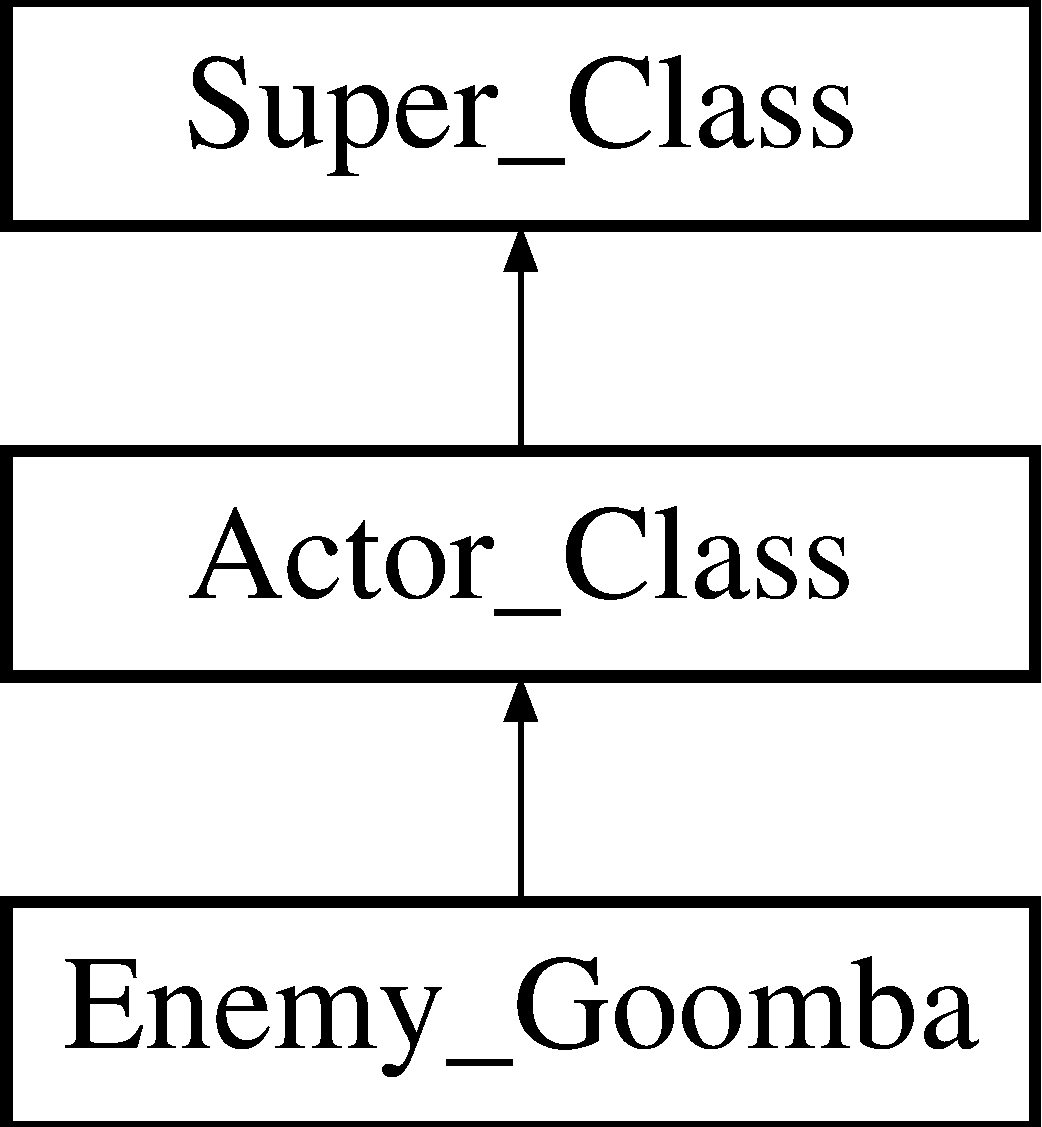
\includegraphics[height=3.000000cm]{class_enemy___goomba}
\end{center}
\end{figure}
\subsection*{Public Member Functions}
\begin{DoxyCompactItemize}
\item 
\hyperlink{class_enemy___goomba_af5a9b3d667381890746453f0dfaa50e6}{Enemy\+\_\+\+Goomba} (sf\+::\+Render\+Window \&window, \hyperlink{class_collision}{Collision} \hyperlink{class_enemy___goomba_a435110bcd5fc30fd2ff0a0d9347c49f3}{col}, int x\+Inn, int y\+Inn)
\item 
void \hyperlink{class_enemy___goomba_ab07621304a0b92c4559679071c060439}{jump} ()
\item 
void \hyperlink{class_enemy___goomba_a0b72ff73bb4f64d4c659a5142862fd1f}{move} ()
\item 
void \hyperlink{class_enemy___goomba_a1947885e29f42889e42947462a9caeb3}{draw} ()
\item 
void \hyperlink{class_enemy___goomba_a09cd52bddf5aa44b94d85adeefa46620}{death} ()
\end{DoxyCompactItemize}
\subsection*{Public Attributes}
\begin{DoxyCompactItemize}
\item 
sf\+::\+Music \hyperlink{class_enemy___goomba_ae247248654854e3be4e5cecc6bea1b08}{sound}
\item 
\hyperlink{classanimatonsprites}{animatonsprites} \hyperlink{class_enemy___goomba_a6e754ed916291f62f4ece73a30903f68}{animation}
\item 
sf\+::\+Rectangle\+Shape \hyperlink{class_enemy___goomba_a06e972cccfe94936721859c90729d3f3}{goomba}
\item 
sf\+::\+Render\+Window \& \hyperlink{class_enemy___goomba_ab4eed505739ee97ea1c682c04b642537}{vindu}
\item 
\hyperlink{class_collision}{Collision} \hyperlink{class_enemy___goomba_a435110bcd5fc30fd2ff0a0d9347c49f3}{col}
\item 
float \hyperlink{class_enemy___goomba_a04e563eef4eda0f20083576ceed3669a}{gravity} = 5
\item 
int \hyperlink{class_enemy___goomba_a4f762d1bb68be95f6ed06a25d5f61721}{startX} =400
\begin{DoxyCompactList}\small\item\em float floor =400;//bør byttes ut med at det er localisasjonen den intersecter med en title \end{DoxyCompactList}\item 
int \hyperlink{class_enemy___goomba_a8d459a604218f1a007e8e62ba95dd70a}{startY} =20
\end{DoxyCompactItemize}
\subsection*{Additional Inherited Members}


\subsection{Detailed Description}


Definition at line 14 of file enemy\+\_\+goomba.\+h.



\subsection{Constructor \& Destructor Documentation}
\hypertarget{class_enemy___goomba_af5a9b3d667381890746453f0dfaa50e6}{}\label{class_enemy___goomba_af5a9b3d667381890746453f0dfaa50e6} 
\index{Enemy\+\_\+\+Goomba@{Enemy\+\_\+\+Goomba}!Enemy\+\_\+\+Goomba@{Enemy\+\_\+\+Goomba}}
\index{Enemy\+\_\+\+Goomba@{Enemy\+\_\+\+Goomba}!Enemy\+\_\+\+Goomba@{Enemy\+\_\+\+Goomba}}
\subsubsection{\texorpdfstring{Enemy\+\_\+\+Goomba()}{Enemy\_Goomba()}}
{\footnotesize\ttfamily Enemy\+\_\+\+Goomba\+::\+Enemy\+\_\+\+Goomba (\begin{DoxyParamCaption}\item[{sf\+::\+Render\+Window \&}]{window,  }\item[{\hyperlink{class_collision}{Collision}}]{col,  }\item[{int}]{x\+Inn,  }\item[{int}]{y\+Inn }\end{DoxyParamCaption})}



Definition at line 11 of file enemy\+\_\+goomba.\+cpp.



\subsection{Member Function Documentation}
\hypertarget{class_enemy___goomba_a09cd52bddf5aa44b94d85adeefa46620}{}\label{class_enemy___goomba_a09cd52bddf5aa44b94d85adeefa46620} 
\index{Enemy\+\_\+\+Goomba@{Enemy\+\_\+\+Goomba}!death@{death}}
\index{death@{death}!Enemy\+\_\+\+Goomba@{Enemy\+\_\+\+Goomba}}
\subsubsection{\texorpdfstring{death()}{death()}}
{\footnotesize\ttfamily void Enemy\+\_\+\+Goomba\+::death (\begin{DoxyParamCaption}{ }\end{DoxyParamCaption})\hspace{0.3cm}{\ttfamily [virtual]}}



Reimplemented from \hyperlink{class_actor___class_a9447c6154a674d7e6bdf24ff2874b7a8}{Actor\+\_\+\+Class}.



Definition at line 88 of file enemy\+\_\+goomba.\+cpp.

\hypertarget{class_enemy___goomba_a1947885e29f42889e42947462a9caeb3}{}\label{class_enemy___goomba_a1947885e29f42889e42947462a9caeb3} 
\index{Enemy\+\_\+\+Goomba@{Enemy\+\_\+\+Goomba}!draw@{draw}}
\index{draw@{draw}!Enemy\+\_\+\+Goomba@{Enemy\+\_\+\+Goomba}}
\subsubsection{\texorpdfstring{draw()}{draw()}}
{\footnotesize\ttfamily void Enemy\+\_\+\+Goomba\+::draw (\begin{DoxyParamCaption}{ }\end{DoxyParamCaption})\hspace{0.3cm}{\ttfamily [virtual]}}



Reimplemented from \hyperlink{class_actor___class_ac49cd62be76b4b950ecbe155413f1b64}{Actor\+\_\+\+Class}.



Definition at line 79 of file enemy\+\_\+goomba.\+cpp.

\hypertarget{class_enemy___goomba_ab07621304a0b92c4559679071c060439}{}\label{class_enemy___goomba_ab07621304a0b92c4559679071c060439} 
\index{Enemy\+\_\+\+Goomba@{Enemy\+\_\+\+Goomba}!jump@{jump}}
\index{jump@{jump}!Enemy\+\_\+\+Goomba@{Enemy\+\_\+\+Goomba}}
\subsubsection{\texorpdfstring{jump()}{jump()}}
{\footnotesize\ttfamily void Enemy\+\_\+\+Goomba\+::jump (\begin{DoxyParamCaption}{ }\end{DoxyParamCaption})\hspace{0.3cm}{\ttfamily [virtual]}}



Reimplemented from \hyperlink{class_actor___class_ab33216a3ce0c856bdc16231c71ae35c2}{Actor\+\_\+\+Class}.



Definition at line 86 of file enemy\+\_\+goomba.\+cpp.

\hypertarget{class_enemy___goomba_a0b72ff73bb4f64d4c659a5142862fd1f}{}\label{class_enemy___goomba_a0b72ff73bb4f64d4c659a5142862fd1f} 
\index{Enemy\+\_\+\+Goomba@{Enemy\+\_\+\+Goomba}!move@{move}}
\index{move@{move}!Enemy\+\_\+\+Goomba@{Enemy\+\_\+\+Goomba}}
\subsubsection{\texorpdfstring{move()}{move()}}
{\footnotesize\ttfamily void Enemy\+\_\+\+Goomba\+::move (\begin{DoxyParamCaption}{ }\end{DoxyParamCaption})\hspace{0.3cm}{\ttfamily [virtual]}}



Reimplemented from \hyperlink{class_actor___class_af1764a94c5410ba8476f56553cd2c327}{Actor\+\_\+\+Class}.



Definition at line 47 of file enemy\+\_\+goomba.\+cpp.



\subsection{Member Data Documentation}
\hypertarget{class_enemy___goomba_a6e754ed916291f62f4ece73a30903f68}{}\label{class_enemy___goomba_a6e754ed916291f62f4ece73a30903f68} 
\index{Enemy\+\_\+\+Goomba@{Enemy\+\_\+\+Goomba}!animation@{animation}}
\index{animation@{animation}!Enemy\+\_\+\+Goomba@{Enemy\+\_\+\+Goomba}}
\subsubsection{\texorpdfstring{animation}{animation}}
{\footnotesize\ttfamily \hyperlink{classanimatonsprites}{animatonsprites} Enemy\+\_\+\+Goomba\+::animation}



Definition at line 19 of file enemy\+\_\+goomba.\+h.

\hypertarget{class_enemy___goomba_a435110bcd5fc30fd2ff0a0d9347c49f3}{}\label{class_enemy___goomba_a435110bcd5fc30fd2ff0a0d9347c49f3} 
\index{Enemy\+\_\+\+Goomba@{Enemy\+\_\+\+Goomba}!col@{col}}
\index{col@{col}!Enemy\+\_\+\+Goomba@{Enemy\+\_\+\+Goomba}}
\subsubsection{\texorpdfstring{col}{col}}
{\footnotesize\ttfamily \hyperlink{class_collision}{Collision} Enemy\+\_\+\+Goomba\+::col}



Definition at line 23 of file enemy\+\_\+goomba.\+h.

\hypertarget{class_enemy___goomba_a06e972cccfe94936721859c90729d3f3}{}\label{class_enemy___goomba_a06e972cccfe94936721859c90729d3f3} 
\index{Enemy\+\_\+\+Goomba@{Enemy\+\_\+\+Goomba}!goomba@{goomba}}
\index{goomba@{goomba}!Enemy\+\_\+\+Goomba@{Enemy\+\_\+\+Goomba}}
\subsubsection{\texorpdfstring{goomba}{goomba}}
{\footnotesize\ttfamily sf\+::\+Rectangle\+Shape Enemy\+\_\+\+Goomba\+::goomba}



Definition at line 20 of file enemy\+\_\+goomba.\+h.

\hypertarget{class_enemy___goomba_a04e563eef4eda0f20083576ceed3669a}{}\label{class_enemy___goomba_a04e563eef4eda0f20083576ceed3669a} 
\index{Enemy\+\_\+\+Goomba@{Enemy\+\_\+\+Goomba}!gravity@{gravity}}
\index{gravity@{gravity}!Enemy\+\_\+\+Goomba@{Enemy\+\_\+\+Goomba}}
\subsubsection{\texorpdfstring{gravity}{gravity}}
{\footnotesize\ttfamily float Enemy\+\_\+\+Goomba\+::gravity = 5}



Definition at line 25 of file enemy\+\_\+goomba.\+h.

\hypertarget{class_enemy___goomba_ae247248654854e3be4e5cecc6bea1b08}{}\label{class_enemy___goomba_ae247248654854e3be4e5cecc6bea1b08} 
\index{Enemy\+\_\+\+Goomba@{Enemy\+\_\+\+Goomba}!sound@{sound}}
\index{sound@{sound}!Enemy\+\_\+\+Goomba@{Enemy\+\_\+\+Goomba}}
\subsubsection{\texorpdfstring{sound}{sound}}
{\footnotesize\ttfamily sf\+::\+Music Enemy\+\_\+\+Goomba\+::sound}



Definition at line 18 of file enemy\+\_\+goomba.\+h.

\hypertarget{class_enemy___goomba_a4f762d1bb68be95f6ed06a25d5f61721}{}\label{class_enemy___goomba_a4f762d1bb68be95f6ed06a25d5f61721} 
\index{Enemy\+\_\+\+Goomba@{Enemy\+\_\+\+Goomba}!startX@{startX}}
\index{startX@{startX}!Enemy\+\_\+\+Goomba@{Enemy\+\_\+\+Goomba}}
\subsubsection{\texorpdfstring{startX}{startX}}
{\footnotesize\ttfamily int Enemy\+\_\+\+Goomba\+::startX =400}



float floor =400;//bør byttes ut med at det er localisasjonen den intersecter med en title 



Definition at line 31 of file enemy\+\_\+goomba.\+h.

\hypertarget{class_enemy___goomba_a8d459a604218f1a007e8e62ba95dd70a}{}\label{class_enemy___goomba_a8d459a604218f1a007e8e62ba95dd70a} 
\index{Enemy\+\_\+\+Goomba@{Enemy\+\_\+\+Goomba}!startY@{startY}}
\index{startY@{startY}!Enemy\+\_\+\+Goomba@{Enemy\+\_\+\+Goomba}}
\subsubsection{\texorpdfstring{startY}{startY}}
{\footnotesize\ttfamily int Enemy\+\_\+\+Goomba\+::startY =20}



Definition at line 32 of file enemy\+\_\+goomba.\+h.

\hypertarget{class_enemy___goomba_ab4eed505739ee97ea1c682c04b642537}{}\label{class_enemy___goomba_ab4eed505739ee97ea1c682c04b642537} 
\index{Enemy\+\_\+\+Goomba@{Enemy\+\_\+\+Goomba}!vindu@{vindu}}
\index{vindu@{vindu}!Enemy\+\_\+\+Goomba@{Enemy\+\_\+\+Goomba}}
\subsubsection{\texorpdfstring{vindu}{vindu}}
{\footnotesize\ttfamily sf\+::\+Render\+Window\& Enemy\+\_\+\+Goomba\+::vindu}



Definition at line 22 of file enemy\+\_\+goomba.\+h.



The documentation for this class was generated from the following files\+:\begin{DoxyCompactItemize}
\item 
Actor/enemy/\hyperlink{enemy__goomba_8h}{enemy\+\_\+goomba.\+h}\item 
Actor/enemy/\hyperlink{enemy__goomba_8cpp}{enemy\+\_\+goomba.\+cpp}\end{DoxyCompactItemize}

\hypertarget{class_finnish__tile}{}\section{Finnish\+\_\+tile Class Reference}
\label{class_finnish__tile}\index{Finnish\+\_\+tile@{Finnish\+\_\+tile}}


{\ttfamily \#include $<$Finnish\+\_\+tile.\+h$>$}

Inheritance diagram for Finnish\+\_\+tile\+:\begin{figure}[H]
\begin{center}
\leavevmode
\includegraphics[height=2.000000cm]{class_finnish__tile}
\end{center}
\end{figure}
\subsection*{Public Member Functions}
\begin{DoxyCompactItemize}
\item 
\hyperlink{class_finnish__tile_a82be12031661ef2e48107319d76a1a30}{Finnish\+\_\+tile} (sf\+::\+Vector2f $\ast$\hyperlink{class_super___tile_ad6bcea1fd54f67808f54ba2aacd88596}{nw}, sf\+::\+Vector2f $\ast$\hyperlink{class_super___tile_a55f6d2860da36f13019bd4e0d18364ca}{ne}, sf\+::\+Vector2f $\ast$\hyperlink{class_super___tile_ab384b89a7a631b8b75c4d405c51a23e1}{se}, sf\+::\+Vector2f $\ast$\hyperlink{class_super___tile_abe9efe0c3d1ed440395225843435dfc8}{sw})
\item 
void \hyperlink{class_finnish__tile_a6b20f4db90ec0522efcd766ec6bc0ab2}{import} (\hyperlink{class_tilemap}{Tilemap} $\ast$import\+\_\+map)
\item 
void \hyperlink{class_finnish__tile_a04fae2c808c18027ec8b74915df33220}{impact} (\hyperlink{class_actor___class}{Actor\+\_\+\+Class} $\ast$actor)
\end{DoxyCompactItemize}
\subsection*{Public Attributes}
\begin{DoxyCompactItemize}
\item 
\hyperlink{class_tilemap}{Tilemap} $\ast$ \hyperlink{class_finnish__tile_ae1bc1de931787b9cc0e4752b64518d94}{map}
\item 
\hyperlink{class_config}{Config} \hyperlink{class_finnish__tile_a29a7324c82ba5ca613dec5a346a5ebe0}{conf}
\end{DoxyCompactItemize}


\subsection{Detailed Description}


Definition at line 13 of file Finnish\+\_\+tile.\+h.



\subsection{Constructor \& Destructor Documentation}
\hypertarget{class_finnish__tile_a82be12031661ef2e48107319d76a1a30}{}\label{class_finnish__tile_a82be12031661ef2e48107319d76a1a30} 
\index{Finnish\+\_\+tile@{Finnish\+\_\+tile}!Finnish\+\_\+tile@{Finnish\+\_\+tile}}
\index{Finnish\+\_\+tile@{Finnish\+\_\+tile}!Finnish\+\_\+tile@{Finnish\+\_\+tile}}
\subsubsection{\texorpdfstring{Finnish\+\_\+tile()}{Finnish\_tile()}}
{\footnotesize\ttfamily Finnish\+\_\+tile\+::\+Finnish\+\_\+tile (\begin{DoxyParamCaption}\item[{sf\+::\+Vector2f $\ast$}]{nw,  }\item[{sf\+::\+Vector2f $\ast$}]{ne,  }\item[{sf\+::\+Vector2f $\ast$}]{se,  }\item[{sf\+::\+Vector2f $\ast$}]{sw }\end{DoxyParamCaption})}



Definition at line 11 of file Finnish\+\_\+tile.\+cpp.



\subsection{Member Function Documentation}
\hypertarget{class_finnish__tile_a04fae2c808c18027ec8b74915df33220}{}\label{class_finnish__tile_a04fae2c808c18027ec8b74915df33220} 
\index{Finnish\+\_\+tile@{Finnish\+\_\+tile}!impact@{impact}}
\index{impact@{impact}!Finnish\+\_\+tile@{Finnish\+\_\+tile}}
\subsubsection{\texorpdfstring{impact()}{impact()}}
{\footnotesize\ttfamily void Finnish\+\_\+tile\+::impact (\begin{DoxyParamCaption}\item[{\hyperlink{class_actor___class}{Actor\+\_\+\+Class} $\ast$}]{actor }\end{DoxyParamCaption})\hspace{0.3cm}{\ttfamily [virtual]}}



Reimplemented from \hyperlink{class_super___tile_a7b509383d0d0ad2df0220f7dc4660823}{Super\+\_\+\+Tile}.



Definition at line 23 of file Finnish\+\_\+tile.\+cpp.

\hypertarget{class_finnish__tile_a6b20f4db90ec0522efcd766ec6bc0ab2}{}\label{class_finnish__tile_a6b20f4db90ec0522efcd766ec6bc0ab2} 
\index{Finnish\+\_\+tile@{Finnish\+\_\+tile}!import@{import}}
\index{import@{import}!Finnish\+\_\+tile@{Finnish\+\_\+tile}}
\subsubsection{\texorpdfstring{import()}{import()}}
{\footnotesize\ttfamily void Finnish\+\_\+tile\+::import (\begin{DoxyParamCaption}\item[{\hyperlink{class_tilemap}{Tilemap} $\ast$}]{import\+\_\+map }\end{DoxyParamCaption})}



\subsection{Member Data Documentation}
\hypertarget{class_finnish__tile_a29a7324c82ba5ca613dec5a346a5ebe0}{}\label{class_finnish__tile_a29a7324c82ba5ca613dec5a346a5ebe0} 
\index{Finnish\+\_\+tile@{Finnish\+\_\+tile}!conf@{conf}}
\index{conf@{conf}!Finnish\+\_\+tile@{Finnish\+\_\+tile}}
\subsubsection{\texorpdfstring{conf}{conf}}
{\footnotesize\ttfamily \hyperlink{class_config}{Config} Finnish\+\_\+tile\+::conf}



Definition at line 17 of file Finnish\+\_\+tile.\+h.

\hypertarget{class_finnish__tile_ae1bc1de931787b9cc0e4752b64518d94}{}\label{class_finnish__tile_ae1bc1de931787b9cc0e4752b64518d94} 
\index{Finnish\+\_\+tile@{Finnish\+\_\+tile}!map@{map}}
\index{map@{map}!Finnish\+\_\+tile@{Finnish\+\_\+tile}}
\subsubsection{\texorpdfstring{map}{map}}
{\footnotesize\ttfamily \hyperlink{class_tilemap}{Tilemap}$\ast$ Finnish\+\_\+tile\+::map}



Definition at line 16 of file Finnish\+\_\+tile.\+h.



The documentation for this class was generated from the following files\+:\begin{DoxyCompactItemize}
\item 
Tile/\hyperlink{_finnish__tile_8h}{Finnish\+\_\+tile.\+h}\item 
Tile/\hyperlink{_finnish__tile_8cpp}{Finnish\+\_\+tile.\+cpp}\end{DoxyCompactItemize}

\hypertarget{class_firewall}{}\section{Firewall Class Reference}
\label{class_firewall}\index{Firewall@{Firewall}}


{\ttfamily \#include $<$Firewall.\+h$>$}

Inheritance diagram for Firewall\+:\begin{figure}[H]
\begin{center}
\leavevmode
\includegraphics[height=3.000000cm]{class_firewall}
\end{center}
\end{figure}
\subsection*{Public Member Functions}
\begin{DoxyCompactItemize}
\item 
\hyperlink{class_firewall_a77f12236ebbdcc218d03366774aa9aab}{Firewall} (sf\+::\+Render\+Window \&window, \hyperlink{class_collision}{Collision} \hyperlink{class_firewall_af1c215a26c43f1339ca1247f02f0d91e}{col}, int x\+Inn, int y\+Inn, int length)
\item 
void \hyperlink{class_firewall_ac08bd22ea41caaa8ab269a9b1e0d36aa}{move} ()
\item 
void \hyperlink{class_firewall_a6fd8ce6bf5731d822c0d47ee209dbe8d}{jump} ()
\item 
void \hyperlink{class_firewall_a3e67e39efb0a425acd1f009f86e434ee}{draw} ()
\item 
void \hyperlink{class_firewall_a506013f97478b8937becdac038c45c8e}{death} ()
\item 
void \hyperlink{class_firewall_a035dac1c484fe153ca14710777c617cb}{interaction\+\_\+effect} (\hyperlink{class_actor___class}{Actor\+\_\+\+Class} $\ast$actor)
\item 
void \hyperlink{class_firewall_a21c3c46eaf7bb026b73a77b0288fa232}{interaction} (std\+::vector$<$ \hyperlink{class_actor___class}{Actor\+\_\+\+Class} $\ast$$>$ actor\+\_\+array)
\end{DoxyCompactItemize}
\subsection*{Public Attributes}
\begin{DoxyCompactItemize}
\item 
sf\+::\+Rectangle\+Shape \hyperlink{class_firewall_aeb0bd3471e4a080461e2c4d9c8e64a4b}{firewall}
\item 
sf\+::\+Render\+Window \& \hyperlink{class_firewall_a65ebc11322740e80e12fec7f0789142d}{vindu}
\item 
\hyperlink{class_collision}{Collision} \hyperlink{class_firewall_af1c215a26c43f1339ca1247f02f0d91e}{col}
\item 
int \hyperlink{class_firewall_ad99a69d3d864a94b406d0dd7711abb73}{mylength}
\end{DoxyCompactItemize}
\subsection*{Additional Inherited Members}


\subsection{Detailed Description}


Definition at line 12 of file Firewall.\+h.



\subsection{Constructor \& Destructor Documentation}
\hypertarget{class_firewall_a77f12236ebbdcc218d03366774aa9aab}{}\label{class_firewall_a77f12236ebbdcc218d03366774aa9aab} 
\index{Firewall@{Firewall}!Firewall@{Firewall}}
\index{Firewall@{Firewall}!Firewall@{Firewall}}
\subsubsection{\texorpdfstring{Firewall()}{Firewall()}}
{\footnotesize\ttfamily Firewall\+::\+Firewall (\begin{DoxyParamCaption}\item[{sf\+::\+Render\+Window \&}]{window,  }\item[{\hyperlink{class_collision}{Collision}}]{col,  }\item[{int}]{x\+Inn,  }\item[{int}]{y\+Inn,  }\item[{int}]{length }\end{DoxyParamCaption})}

ensures that the hero texture has been loaded 

Definition at line 10 of file Firewall.\+cpp.



\subsection{Member Function Documentation}
\hypertarget{class_firewall_a506013f97478b8937becdac038c45c8e}{}\label{class_firewall_a506013f97478b8937becdac038c45c8e} 
\index{Firewall@{Firewall}!death@{death}}
\index{death@{death}!Firewall@{Firewall}}
\subsubsection{\texorpdfstring{death()}{death()}}
{\footnotesize\ttfamily void Firewall\+::death (\begin{DoxyParamCaption}{ }\end{DoxyParamCaption})\hspace{0.3cm}{\ttfamily [virtual]}}



Reimplemented from \hyperlink{class_actor___class_a9447c6154a674d7e6bdf24ff2874b7a8}{Actor\+\_\+\+Class}.



Definition at line 76 of file Firewall.\+cpp.

\hypertarget{class_firewall_a3e67e39efb0a425acd1f009f86e434ee}{}\label{class_firewall_a3e67e39efb0a425acd1f009f86e434ee} 
\index{Firewall@{Firewall}!draw@{draw}}
\index{draw@{draw}!Firewall@{Firewall}}
\subsubsection{\texorpdfstring{draw()}{draw()}}
{\footnotesize\ttfamily void Firewall\+::draw (\begin{DoxyParamCaption}{ }\end{DoxyParamCaption})\hspace{0.3cm}{\ttfamily [virtual]}}



Reimplemented from \hyperlink{class_actor___class_ac49cd62be76b4b950ecbe155413f1b64}{Actor\+\_\+\+Class}.



Definition at line 68 of file Firewall.\+cpp.

\hypertarget{class_firewall_a21c3c46eaf7bb026b73a77b0288fa232}{}\label{class_firewall_a21c3c46eaf7bb026b73a77b0288fa232} 
\index{Firewall@{Firewall}!interaction@{interaction}}
\index{interaction@{interaction}!Firewall@{Firewall}}
\subsubsection{\texorpdfstring{interaction()}{interaction()}}
{\footnotesize\ttfamily void Firewall\+::interaction (\begin{DoxyParamCaption}\item[{std\+::vector$<$ \hyperlink{class_actor___class}{Actor\+\_\+\+Class} $\ast$$>$}]{actor\+\_\+array }\end{DoxyParamCaption})\hspace{0.3cm}{\ttfamily [virtual]}}



Reimplemented from \hyperlink{class_actor___class_a87d1e079d8576fa99592a60b38a04a1b}{Actor\+\_\+\+Class}.



Definition at line 60 of file Firewall.\+cpp.

\hypertarget{class_firewall_a035dac1c484fe153ca14710777c617cb}{}\label{class_firewall_a035dac1c484fe153ca14710777c617cb} 
\index{Firewall@{Firewall}!interaction\+\_\+effect@{interaction\+\_\+effect}}
\index{interaction\+\_\+effect@{interaction\+\_\+effect}!Firewall@{Firewall}}
\subsubsection{\texorpdfstring{interaction\+\_\+effect()}{interaction\_effect()}}
{\footnotesize\ttfamily void Firewall\+::interaction\+\_\+effect (\begin{DoxyParamCaption}\item[{\hyperlink{class_actor___class}{Actor\+\_\+\+Class} $\ast$}]{actor }\end{DoxyParamCaption})\hspace{0.3cm}{\ttfamily [virtual]}}



Reimplemented from \hyperlink{class_actor___class_af3488ca470eb77255060142fd167aa72}{Actor\+\_\+\+Class}.



Definition at line 81 of file Firewall.\+cpp.

\hypertarget{class_firewall_a6fd8ce6bf5731d822c0d47ee209dbe8d}{}\label{class_firewall_a6fd8ce6bf5731d822c0d47ee209dbe8d} 
\index{Firewall@{Firewall}!jump@{jump}}
\index{jump@{jump}!Firewall@{Firewall}}
\subsubsection{\texorpdfstring{jump()}{jump()}}
{\footnotesize\ttfamily void Firewall\+::jump (\begin{DoxyParamCaption}{ }\end{DoxyParamCaption})\hspace{0.3cm}{\ttfamily [virtual]}}



Reimplemented from \hyperlink{class_actor___class_ab33216a3ce0c856bdc16231c71ae35c2}{Actor\+\_\+\+Class}.



Definition at line 73 of file Firewall.\+cpp.

\hypertarget{class_firewall_ac08bd22ea41caaa8ab269a9b1e0d36aa}{}\label{class_firewall_ac08bd22ea41caaa8ab269a9b1e0d36aa} 
\index{Firewall@{Firewall}!move@{move}}
\index{move@{move}!Firewall@{Firewall}}
\subsubsection{\texorpdfstring{move()}{move()}}
{\footnotesize\ttfamily void Firewall\+::move (\begin{DoxyParamCaption}{ }\end{DoxyParamCaption})\hspace{0.3cm}{\ttfamily [virtual]}}



Reimplemented from \hyperlink{class_actor___class_af1764a94c5410ba8476f56553cd2c327}{Actor\+\_\+\+Class}.



Definition at line 49 of file Firewall.\+cpp.



\subsection{Member Data Documentation}
\hypertarget{class_firewall_af1c215a26c43f1339ca1247f02f0d91e}{}\label{class_firewall_af1c215a26c43f1339ca1247f02f0d91e} 
\index{Firewall@{Firewall}!col@{col}}
\index{col@{col}!Firewall@{Firewall}}
\subsubsection{\texorpdfstring{col}{col}}
{\footnotesize\ttfamily \hyperlink{class_collision}{Collision} Firewall\+::col}



Definition at line 18 of file Firewall.\+h.

\hypertarget{class_firewall_aeb0bd3471e4a080461e2c4d9c8e64a4b}{}\label{class_firewall_aeb0bd3471e4a080461e2c4d9c8e64a4b} 
\index{Firewall@{Firewall}!firewall@{firewall}}
\index{firewall@{firewall}!Firewall@{Firewall}}
\subsubsection{\texorpdfstring{firewall}{firewall}}
{\footnotesize\ttfamily sf\+::\+Rectangle\+Shape Firewall\+::firewall}



Definition at line 15 of file Firewall.\+h.

\hypertarget{class_firewall_ad99a69d3d864a94b406d0dd7711abb73}{}\label{class_firewall_ad99a69d3d864a94b406d0dd7711abb73} 
\index{Firewall@{Firewall}!mylength@{mylength}}
\index{mylength@{mylength}!Firewall@{Firewall}}
\subsubsection{\texorpdfstring{mylength}{mylength}}
{\footnotesize\ttfamily int Firewall\+::mylength}



Definition at line 19 of file Firewall.\+h.

\hypertarget{class_firewall_a65ebc11322740e80e12fec7f0789142d}{}\label{class_firewall_a65ebc11322740e80e12fec7f0789142d} 
\index{Firewall@{Firewall}!vindu@{vindu}}
\index{vindu@{vindu}!Firewall@{Firewall}}
\subsubsection{\texorpdfstring{vindu}{vindu}}
{\footnotesize\ttfamily sf\+::\+Render\+Window\& Firewall\+::vindu}



Definition at line 17 of file Firewall.\+h.



The documentation for this class was generated from the following files\+:\begin{DoxyCompactItemize}
\item 
Actor/enemy/\hyperlink{_firewall_8h}{Firewall.\+h}\item 
Actor/enemy/\hyperlink{_firewall_8cpp}{Firewall.\+cpp}\end{DoxyCompactItemize}

\hypertarget{class_flying__enemy}{}\section{Flying\+\_\+enemy Class Reference}
\label{class_flying__enemy}\index{Flying\+\_\+enemy@{Flying\+\_\+enemy}}


{\ttfamily \#include $<$Flying\+\_\+enemy.\+h$>$}

Inheritance diagram for Flying\+\_\+enemy\+:\begin{figure}[H]
\begin{center}
\leavevmode
\includegraphics[height=3.000000cm]{class_flying__enemy}
\end{center}
\end{figure}
\subsection*{Public Member Functions}
\begin{DoxyCompactItemize}
\item 
\hyperlink{class_flying__enemy_a2421fcde96321136c07dff8ad05f459b}{Flying\+\_\+enemy} (sf\+::\+Render\+Window \&window, \hyperlink{class_collision}{Collision} \hyperlink{class_flying__enemy_a4fc05425448f4272839d9765f5f9e859}{col}, int x\+Inn, int y\+Inn, \hyperlink{class_config}{Config} \&conf)
\item 
void \hyperlink{class_flying__enemy_a0b55c3bf770b7f94fa6892cac47c80bd}{move} ()
\item 
void \hyperlink{class_flying__enemy_af9f8bc6cf140ee0c4ce1f7e340ef79e5}{jump} ()
\item 
void \hyperlink{class_flying__enemy_a2d8bc9f4c82ec045da7346bd3613bfcb}{draw} ()
\item 
void \hyperlink{class_flying__enemy_a79631d3c3cf673c0651be53eac8ac330}{death} ()
\end{DoxyCompactItemize}
\subsection*{Public Attributes}
\begin{DoxyCompactItemize}
\item 
sf\+::\+Music \hyperlink{class_flying__enemy_a4b51b8962f740ad0357420758e19d9c9}{sound}
\item 
sf\+::\+Rectangle\+Shape \hyperlink{class_flying__enemy_a4c36026231ab03d14c8b3429c026c2ad}{corrupt\+\_\+file}
\item 
sf\+::\+Render\+Window \& \hyperlink{class_flying__enemy_a27b52e8aef1f1164bf61e8ef0d16428c}{vindu}
\item 
\hyperlink{class_collision}{Collision} \hyperlink{class_flying__enemy_a4fc05425448f4272839d9765f5f9e859}{col}
\end{DoxyCompactItemize}
\subsection*{Additional Inherited Members}


\subsection{Detailed Description}


Definition at line 13 of file Flying\+\_\+enemy.\+h.



\subsection{Constructor \& Destructor Documentation}
\hypertarget{class_flying__enemy_a2421fcde96321136c07dff8ad05f459b}{}\label{class_flying__enemy_a2421fcde96321136c07dff8ad05f459b} 
\index{Flying\+\_\+enemy@{Flying\+\_\+enemy}!Flying\+\_\+enemy@{Flying\+\_\+enemy}}
\index{Flying\+\_\+enemy@{Flying\+\_\+enemy}!Flying\+\_\+enemy@{Flying\+\_\+enemy}}
\subsubsection{\texorpdfstring{Flying\+\_\+enemy()}{Flying\_enemy()}}
{\footnotesize\ttfamily Flying\+\_\+enemy\+::\+Flying\+\_\+enemy (\begin{DoxyParamCaption}\item[{sf\+::\+Render\+Window \&}]{window,  }\item[{\hyperlink{class_collision}{Collision}}]{col,  }\item[{int}]{x\+Inn,  }\item[{int}]{y\+Inn,  }\item[{\hyperlink{class_config}{Config} \&}]{conf }\end{DoxyParamCaption})}

ensures that the hero texture has been loaded 

Definition at line 7 of file Flying\+\_\+enemy.\+cpp.



\subsection{Member Function Documentation}
\hypertarget{class_flying__enemy_a79631d3c3cf673c0651be53eac8ac330}{}\label{class_flying__enemy_a79631d3c3cf673c0651be53eac8ac330} 
\index{Flying\+\_\+enemy@{Flying\+\_\+enemy}!death@{death}}
\index{death@{death}!Flying\+\_\+enemy@{Flying\+\_\+enemy}}
\subsubsection{\texorpdfstring{death()}{death()}}
{\footnotesize\ttfamily void Flying\+\_\+enemy\+::death (\begin{DoxyParamCaption}{ }\end{DoxyParamCaption})\hspace{0.3cm}{\ttfamily [virtual]}}



Reimplemented from \hyperlink{class_actor___class_a9447c6154a674d7e6bdf24ff2874b7a8}{Actor\+\_\+\+Class}.



Definition at line 92 of file Flying\+\_\+enemy.\+cpp.

\hypertarget{class_flying__enemy_a2d8bc9f4c82ec045da7346bd3613bfcb}{}\label{class_flying__enemy_a2d8bc9f4c82ec045da7346bd3613bfcb} 
\index{Flying\+\_\+enemy@{Flying\+\_\+enemy}!draw@{draw}}
\index{draw@{draw}!Flying\+\_\+enemy@{Flying\+\_\+enemy}}
\subsubsection{\texorpdfstring{draw()}{draw()}}
{\footnotesize\ttfamily void Flying\+\_\+enemy\+::draw (\begin{DoxyParamCaption}{ }\end{DoxyParamCaption})\hspace{0.3cm}{\ttfamily [virtual]}}



Reimplemented from \hyperlink{class_actor___class_ac49cd62be76b4b950ecbe155413f1b64}{Actor\+\_\+\+Class}.



Definition at line 103 of file Flying\+\_\+enemy.\+cpp.

\hypertarget{class_flying__enemy_af9f8bc6cf140ee0c4ce1f7e340ef79e5}{}\label{class_flying__enemy_af9f8bc6cf140ee0c4ce1f7e340ef79e5} 
\index{Flying\+\_\+enemy@{Flying\+\_\+enemy}!jump@{jump}}
\index{jump@{jump}!Flying\+\_\+enemy@{Flying\+\_\+enemy}}
\subsubsection{\texorpdfstring{jump()}{jump()}}
{\footnotesize\ttfamily void Flying\+\_\+enemy\+::jump (\begin{DoxyParamCaption}{ }\end{DoxyParamCaption})\hspace{0.3cm}{\ttfamily [virtual]}}



Reimplemented from \hyperlink{class_actor___class_ab33216a3ce0c856bdc16231c71ae35c2}{Actor\+\_\+\+Class}.



Definition at line 108 of file Flying\+\_\+enemy.\+cpp.

\hypertarget{class_flying__enemy_a0b55c3bf770b7f94fa6892cac47c80bd}{}\label{class_flying__enemy_a0b55c3bf770b7f94fa6892cac47c80bd} 
\index{Flying\+\_\+enemy@{Flying\+\_\+enemy}!move@{move}}
\index{move@{move}!Flying\+\_\+enemy@{Flying\+\_\+enemy}}
\subsubsection{\texorpdfstring{move()}{move()}}
{\footnotesize\ttfamily void Flying\+\_\+enemy\+::move (\begin{DoxyParamCaption}{ }\end{DoxyParamCaption})\hspace{0.3cm}{\ttfamily [virtual]}}



Reimplemented from \hyperlink{class_actor___class_af1764a94c5410ba8476f56553cd2c327}{Actor\+\_\+\+Class}.



Definition at line 51 of file Flying\+\_\+enemy.\+cpp.



\subsection{Member Data Documentation}
\hypertarget{class_flying__enemy_a4fc05425448f4272839d9765f5f9e859}{}\label{class_flying__enemy_a4fc05425448f4272839d9765f5f9e859} 
\index{Flying\+\_\+enemy@{Flying\+\_\+enemy}!col@{col}}
\index{col@{col}!Flying\+\_\+enemy@{Flying\+\_\+enemy}}
\subsubsection{\texorpdfstring{col}{col}}
{\footnotesize\ttfamily \hyperlink{class_collision}{Collision} Flying\+\_\+enemy\+::col}



Definition at line 20 of file Flying\+\_\+enemy.\+h.

\hypertarget{class_flying__enemy_a4c36026231ab03d14c8b3429c026c2ad}{}\label{class_flying__enemy_a4c36026231ab03d14c8b3429c026c2ad} 
\index{Flying\+\_\+enemy@{Flying\+\_\+enemy}!corrupt\+\_\+file@{corrupt\+\_\+file}}
\index{corrupt\+\_\+file@{corrupt\+\_\+file}!Flying\+\_\+enemy@{Flying\+\_\+enemy}}
\subsubsection{\texorpdfstring{corrupt\+\_\+file}{corrupt\_file}}
{\footnotesize\ttfamily sf\+::\+Rectangle\+Shape Flying\+\_\+enemy\+::corrupt\+\_\+file}



Definition at line 17 of file Flying\+\_\+enemy.\+h.

\hypertarget{class_flying__enemy_a4b51b8962f740ad0357420758e19d9c9}{}\label{class_flying__enemy_a4b51b8962f740ad0357420758e19d9c9} 
\index{Flying\+\_\+enemy@{Flying\+\_\+enemy}!sound@{sound}}
\index{sound@{sound}!Flying\+\_\+enemy@{Flying\+\_\+enemy}}
\subsubsection{\texorpdfstring{sound}{sound}}
{\footnotesize\ttfamily sf\+::\+Music Flying\+\_\+enemy\+::sound}



Definition at line 16 of file Flying\+\_\+enemy.\+h.

\hypertarget{class_flying__enemy_a27b52e8aef1f1164bf61e8ef0d16428c}{}\label{class_flying__enemy_a27b52e8aef1f1164bf61e8ef0d16428c} 
\index{Flying\+\_\+enemy@{Flying\+\_\+enemy}!vindu@{vindu}}
\index{vindu@{vindu}!Flying\+\_\+enemy@{Flying\+\_\+enemy}}
\subsubsection{\texorpdfstring{vindu}{vindu}}
{\footnotesize\ttfamily sf\+::\+Render\+Window\& Flying\+\_\+enemy\+::vindu}



Definition at line 19 of file Flying\+\_\+enemy.\+h.



The documentation for this class was generated from the following files\+:\begin{DoxyCompactItemize}
\item 
Actor/enemy/\hyperlink{_flying__enemy_8h}{Flying\+\_\+enemy.\+h}\item 
Actor/enemy/\hyperlink{_flying__enemy_8cpp}{Flying\+\_\+enemy.\+cpp}\end{DoxyCompactItemize}

\hypertarget{class_game___state}{}\section{Game\+\_\+\+State Class Reference}
\label{class_game___state}\index{Game\+\_\+\+State@{Game\+\_\+\+State}}


{\ttfamily \#include $<$game\+\_\+state.\+h$>$}

Inheritance diagram for Game\+\_\+\+State\+:\begin{figure}[H]
\begin{center}
\leavevmode
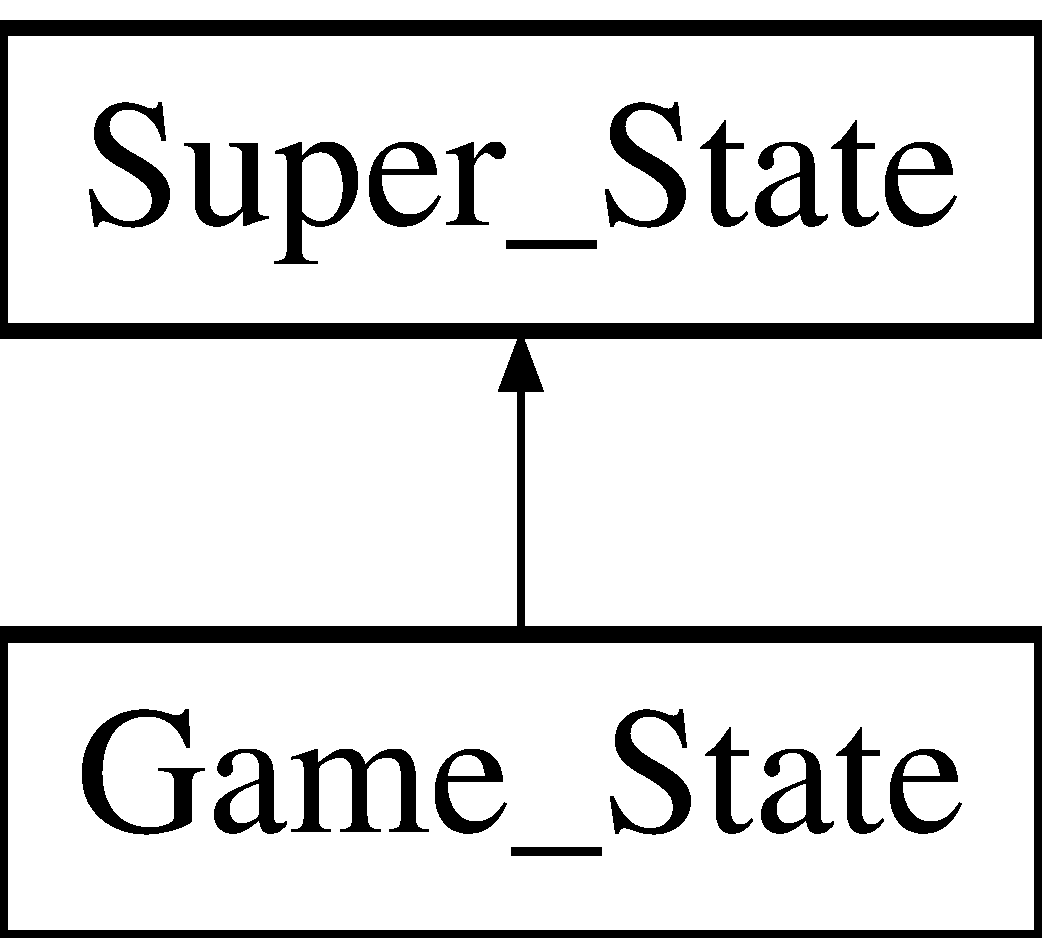
\includegraphics[height=2.000000cm]{class_game___state}
\end{center}
\end{figure}
\subsection*{Public Member Functions}
\begin{DoxyCompactItemize}
\item 
\hyperlink{class_game___state_a93409470dc62892876fe0dafafb910ad}{Game\+\_\+\+State} (sf\+::\+Render\+Window \&\hyperlink{class_game___state_a5a9bb4b732ee25b0f9de3baa2ee71045}{window}, int \hyperlink{class_super___state_ad6b74d4864a4e2cccf58316cd1af2e83}{level}, \hyperlink{class_config}{Config} \&\hyperlink{class_game___state_a6f82c6c66962953aee7de556d3877eeb}{conf}, sf\+::\+View \&camera)
\item 
void \hyperlink{class_game___state_aaaaa14909458922108ecc2495986db3d}{switch\+To} ()
\item 
bool \hyperlink{class_game___state_acf99f3862148f13c48e9644b7bd5e64b}{switch\+Level} (\hyperlink{class_tilemap}{Tilemap} $\ast$\hyperlink{class_game___state_af09e995b6bf08cbc23ef6dc4b32ad5cd}{map}, std\+::vector$<$ \hyperlink{class_level}{Level} $>$ level\+Loc\+Array, bool test, \hyperlink{class_config}{Config} $\ast$\hyperlink{class_game___state_a6f82c6c66962953aee7de556d3877eeb}{conf}, int \hyperlink{class_super___state_ad6b74d4864a4e2cccf58316cd1af2e83}{level})
\item 
void \hyperlink{class_game___state_a122037a320f91a566d07697ea4fa0f39}{Firewall\+Cam} (int firewallX)
\item 
sf\+::\+View \hyperlink{class_game___state_a87ce59fa6d8147096bfb835c5a93fc1d}{cam\+Mov} (sf\+::\+View camera, \hyperlink{class_hero}{Hero} helt)
\item 
\hyperlink{class_collision}{Collision} \hyperlink{class_game___state_a828b93b20d67bb6bdb1d15cd538157f5}{spawn} (\hyperlink{class_collision}{Collision} col)
\item 
void \hyperlink{class_game___state_a8dad75e154735be07e6d8d257bda049f}{actor\+Act} ()
\end{DoxyCompactItemize}
\subsection*{Public Attributes}
\begin{DoxyCompactItemize}
\item 
sf\+::\+Music \hyperlink{class_game___state_a3e529295cb321b91f68594e06ee5f8de}{B\+GM}
\end{DoxyCompactItemize}
\subsection*{Protected Attributes}
\begin{DoxyCompactItemize}
\item 
bool \hyperlink{class_game___state_a173b2606fcaf010b8f1eb8b6e5487a4e}{key\+Test}
\item 
bool \hyperlink{class_game___state_a6da4c593a72687a91c91027463fb9083}{firewall\+Test} = false
\item 
bool \hyperlink{class_game___state_a0e432196bf012dbfa928c947d829ae69}{firewall\+Level} = false
\item 
int \hyperlink{class_game___state_ab7f247337f6c29608333e2c8fe79b973}{last\+FirewallX}
\item 
int \hyperlink{class_game___state_a6aef3b71ebbfc46aabe99005ad609c96}{shake\+Var} = 0
\item 
int \hyperlink{class_game___state_a24adb6b7cfae8390f484501af0835b3f}{kameraX}
\item 
int \hyperlink{class_game___state_ad4fc3a4ab3d6caf08cfc8ae92505ebd6}{kameraY}
\item 
int \hyperlink{class_game___state_a800d81a46d0b4dead0b3516ab24ebc9c}{kamera\+Pos} = 0
\item 
int \hyperlink{class_game___state_abbd68113ae4a7ed42d4e600edd857ef1}{kamera\+Speed} = 5
\item 
int \hyperlink{class_game___state_aea29b5ae20f29dea3ba382e0f406319e}{spawning\+Actor} = 1
\item 
int \hyperlink{class_game___state_ab3f5efd3966eb17cff370700a750e1de}{spawning\+Enemy\+Type}
\item 
\hyperlink{class_tilemap}{Tilemap} \hyperlink{class_game___state_af09e995b6bf08cbc23ef6dc4b32ad5cd}{map}
\item 
\hyperlink{class_tilemap}{Tilemap} \hyperlink{class_game___state_a9de848045ff6eb1a2a2548a82fcd87b5}{map2}
\item 
\hyperlink{class_config}{Config} \& \hyperlink{class_game___state_a6f82c6c66962953aee7de556d3877eeb}{conf}
\item 
sf\+::\+Render\+Window \& \hyperlink{class_game___state_a5a9bb4b732ee25b0f9de3baa2ee71045}{window}
\item 
std\+::vector$<$ \hyperlink{class_actor___class}{Actor\+\_\+\+Class} $\ast$ $>$ \hyperlink{class_game___state_a5b5ad0c10282bbb7e407ccbba8a7c213}{actor\+\_\+array}
\item 
sf\+::\+View \hyperlink{class_game___state_a041c421a58505094d2dfc07f8a055e45}{camera2}
\end{DoxyCompactItemize}


\subsection{Detailed Description}


Definition at line 15 of file game\+\_\+state.\+h.



\subsection{Constructor \& Destructor Documentation}
\hypertarget{class_game___state_a93409470dc62892876fe0dafafb910ad}{}\label{class_game___state_a93409470dc62892876fe0dafafb910ad} 
\index{Game\+\_\+\+State@{Game\+\_\+\+State}!Game\+\_\+\+State@{Game\+\_\+\+State}}
\index{Game\+\_\+\+State@{Game\+\_\+\+State}!Game\+\_\+\+State@{Game\+\_\+\+State}}
\subsubsection{\texorpdfstring{Game\+\_\+\+State()}{Game\_State()}}
{\footnotesize\ttfamily Game\+\_\+\+State\+::\+Game\+\_\+\+State (\begin{DoxyParamCaption}\item[{sf\+::\+Render\+Window \&}]{window,  }\item[{int}]{level,  }\item[{\hyperlink{class_config}{Config} \&}]{conf,  }\item[{sf\+::\+View \&}]{camera }\end{DoxyParamCaption})}

constructs the game\+\_\+state 
\begin{DoxyParams}{Parameters}
{\em window} & window gamestate is drawn in \\
\hline
\end{DoxyParams}
\begin{DoxyReturn}{Returns}

\end{DoxyReturn}


Definition at line 29 of file game\+\_\+state.\+cpp.



\subsection{Member Function Documentation}
\hypertarget{class_game___state_a8dad75e154735be07e6d8d257bda049f}{}\label{class_game___state_a8dad75e154735be07e6d8d257bda049f} 
\index{Game\+\_\+\+State@{Game\+\_\+\+State}!actor\+Act@{actor\+Act}}
\index{actor\+Act@{actor\+Act}!Game\+\_\+\+State@{Game\+\_\+\+State}}
\subsubsection{\texorpdfstring{actor\+Act()}{actorAct()}}
{\footnotesize\ttfamily void Game\+\_\+\+State\+::actor\+Act (\begin{DoxyParamCaption}{ }\end{DoxyParamCaption})}



Definition at line 232 of file game\+\_\+state.\+cpp.

\hypertarget{class_game___state_a87ce59fa6d8147096bfb835c5a93fc1d}{}\label{class_game___state_a87ce59fa6d8147096bfb835c5a93fc1d} 
\index{Game\+\_\+\+State@{Game\+\_\+\+State}!cam\+Mov@{cam\+Mov}}
\index{cam\+Mov@{cam\+Mov}!Game\+\_\+\+State@{Game\+\_\+\+State}}
\subsubsection{\texorpdfstring{cam\+Mov()}{camMov()}}
{\footnotesize\ttfamily sf\+::\+View Game\+\_\+\+State\+::cam\+Mov (\begin{DoxyParamCaption}\item[{sf\+::\+View}]{camera,  }\item[{\hyperlink{class_hero}{Hero}}]{helt }\end{DoxyParamCaption})}



Definition at line 362 of file game\+\_\+state.\+cpp.

\hypertarget{class_game___state_a122037a320f91a566d07697ea4fa0f39}{}\label{class_game___state_a122037a320f91a566d07697ea4fa0f39} 
\index{Game\+\_\+\+State@{Game\+\_\+\+State}!Firewall\+Cam@{Firewall\+Cam}}
\index{Firewall\+Cam@{Firewall\+Cam}!Game\+\_\+\+State@{Game\+\_\+\+State}}
\subsubsection{\texorpdfstring{Firewall\+Cam()}{FirewallCam()}}
{\footnotesize\ttfamily void Game\+\_\+\+State\+::\+Firewall\+Cam (\begin{DoxyParamCaption}\item[{int}]{firewallX }\end{DoxyParamCaption})}



Definition at line 410 of file game\+\_\+state.\+cpp.

\hypertarget{class_game___state_a828b93b20d67bb6bdb1d15cd538157f5}{}\label{class_game___state_a828b93b20d67bb6bdb1d15cd538157f5} 
\index{Game\+\_\+\+State@{Game\+\_\+\+State}!spawn@{spawn}}
\index{spawn@{spawn}!Game\+\_\+\+State@{Game\+\_\+\+State}}
\subsubsection{\texorpdfstring{spawn()}{spawn()}}
{\footnotesize\ttfamily \hyperlink{class_collision}{Collision} Game\+\_\+\+State\+::spawn (\begin{DoxyParamCaption}\item[{\hyperlink{class_collision}{Collision}}]{col }\end{DoxyParamCaption})}



Definition at line 268 of file game\+\_\+state.\+cpp.

\hypertarget{class_game___state_acf99f3862148f13c48e9644b7bd5e64b}{}\label{class_game___state_acf99f3862148f13c48e9644b7bd5e64b} 
\index{Game\+\_\+\+State@{Game\+\_\+\+State}!switch\+Level@{switch\+Level}}
\index{switch\+Level@{switch\+Level}!Game\+\_\+\+State@{Game\+\_\+\+State}}
\subsubsection{\texorpdfstring{switch\+Level()}{switchLevel()}}
{\footnotesize\ttfamily bool Game\+\_\+\+State\+::switch\+Level (\begin{DoxyParamCaption}\item[{\hyperlink{class_tilemap}{Tilemap} $\ast$}]{map,  }\item[{std\+::vector$<$ \hyperlink{class_level}{Level} $>$}]{level\+Loc\+Array,  }\item[{bool}]{test,  }\item[{\hyperlink{class_config}{Config} $\ast$}]{conf,  }\item[{int}]{level }\end{DoxyParamCaption})}



Definition at line 423 of file game\+\_\+state.\+cpp.

\hypertarget{class_game___state_aaaaa14909458922108ecc2495986db3d}{}\label{class_game___state_aaaaa14909458922108ecc2495986db3d} 
\index{Game\+\_\+\+State@{Game\+\_\+\+State}!switch\+To@{switch\+To}}
\index{switch\+To@{switch\+To}!Game\+\_\+\+State@{Game\+\_\+\+State}}
\subsubsection{\texorpdfstring{switch\+To()}{switchTo()}}
{\footnotesize\ttfamily void Game\+\_\+\+State\+::switch\+To (\begin{DoxyParamCaption}{ }\end{DoxyParamCaption})}



Definition at line 266 of file game\+\_\+state.\+cpp.



\subsection{Member Data Documentation}
\hypertarget{class_game___state_a5b5ad0c10282bbb7e407ccbba8a7c213}{}\label{class_game___state_a5b5ad0c10282bbb7e407ccbba8a7c213} 
\index{Game\+\_\+\+State@{Game\+\_\+\+State}!actor\+\_\+array@{actor\+\_\+array}}
\index{actor\+\_\+array@{actor\+\_\+array}!Game\+\_\+\+State@{Game\+\_\+\+State}}
\subsubsection{\texorpdfstring{actor\+\_\+array}{actor\_array}}
{\footnotesize\ttfamily std\+::vector$<$\hyperlink{class_actor___class}{Actor\+\_\+\+Class}$\ast$$>$ Game\+\_\+\+State\+::actor\+\_\+array\hspace{0.3cm}{\ttfamily [protected]}}



Definition at line 46 of file game\+\_\+state.\+h.

\hypertarget{class_game___state_a3e529295cb321b91f68594e06ee5f8de}{}\label{class_game___state_a3e529295cb321b91f68594e06ee5f8de} 
\index{Game\+\_\+\+State@{Game\+\_\+\+State}!B\+GM@{B\+GM}}
\index{B\+GM@{B\+GM}!Game\+\_\+\+State@{Game\+\_\+\+State}}
\subsubsection{\texorpdfstring{B\+GM}{BGM}}
{\footnotesize\ttfamily sf\+::\+Music Game\+\_\+\+State\+::\+B\+GM}



Definition at line 23 of file game\+\_\+state.\+h.

\hypertarget{class_game___state_a041c421a58505094d2dfc07f8a055e45}{}\label{class_game___state_a041c421a58505094d2dfc07f8a055e45} 
\index{Game\+\_\+\+State@{Game\+\_\+\+State}!camera2@{camera2}}
\index{camera2@{camera2}!Game\+\_\+\+State@{Game\+\_\+\+State}}
\subsubsection{\texorpdfstring{camera2}{camera2}}
{\footnotesize\ttfamily sf\+::\+View Game\+\_\+\+State\+::camera2\hspace{0.3cm}{\ttfamily [protected]}}



Definition at line 47 of file game\+\_\+state.\+h.

\hypertarget{class_game___state_a6f82c6c66962953aee7de556d3877eeb}{}\label{class_game___state_a6f82c6c66962953aee7de556d3877eeb} 
\index{Game\+\_\+\+State@{Game\+\_\+\+State}!conf@{conf}}
\index{conf@{conf}!Game\+\_\+\+State@{Game\+\_\+\+State}}
\subsubsection{\texorpdfstring{conf}{conf}}
{\footnotesize\ttfamily \hyperlink{class_config}{Config}\& Game\+\_\+\+State\+::conf\hspace{0.3cm}{\ttfamily [protected]}}



Definition at line 44 of file game\+\_\+state.\+h.

\hypertarget{class_game___state_a0e432196bf012dbfa928c947d829ae69}{}\label{class_game___state_a0e432196bf012dbfa928c947d829ae69} 
\index{Game\+\_\+\+State@{Game\+\_\+\+State}!firewall\+Level@{firewall\+Level}}
\index{firewall\+Level@{firewall\+Level}!Game\+\_\+\+State@{Game\+\_\+\+State}}
\subsubsection{\texorpdfstring{firewall\+Level}{firewallLevel}}
{\footnotesize\ttfamily bool Game\+\_\+\+State\+::firewall\+Level = false\hspace{0.3cm}{\ttfamily [protected]}}



Definition at line 33 of file game\+\_\+state.\+h.

\hypertarget{class_game___state_a6da4c593a72687a91c91027463fb9083}{}\label{class_game___state_a6da4c593a72687a91c91027463fb9083} 
\index{Game\+\_\+\+State@{Game\+\_\+\+State}!firewall\+Test@{firewall\+Test}}
\index{firewall\+Test@{firewall\+Test}!Game\+\_\+\+State@{Game\+\_\+\+State}}
\subsubsection{\texorpdfstring{firewall\+Test}{firewallTest}}
{\footnotesize\ttfamily bool Game\+\_\+\+State\+::firewall\+Test = false\hspace{0.3cm}{\ttfamily [protected]}}



Definition at line 32 of file game\+\_\+state.\+h.

\hypertarget{class_game___state_a800d81a46d0b4dead0b3516ab24ebc9c}{}\label{class_game___state_a800d81a46d0b4dead0b3516ab24ebc9c} 
\index{Game\+\_\+\+State@{Game\+\_\+\+State}!kamera\+Pos@{kamera\+Pos}}
\index{kamera\+Pos@{kamera\+Pos}!Game\+\_\+\+State@{Game\+\_\+\+State}}
\subsubsection{\texorpdfstring{kamera\+Pos}{kameraPos}}
{\footnotesize\ttfamily int Game\+\_\+\+State\+::kamera\+Pos = 0\hspace{0.3cm}{\ttfamily [protected]}}



Definition at line 38 of file game\+\_\+state.\+h.

\hypertarget{class_game___state_abbd68113ae4a7ed42d4e600edd857ef1}{}\label{class_game___state_abbd68113ae4a7ed42d4e600edd857ef1} 
\index{Game\+\_\+\+State@{Game\+\_\+\+State}!kamera\+Speed@{kamera\+Speed}}
\index{kamera\+Speed@{kamera\+Speed}!Game\+\_\+\+State@{Game\+\_\+\+State}}
\subsubsection{\texorpdfstring{kamera\+Speed}{kameraSpeed}}
{\footnotesize\ttfamily int Game\+\_\+\+State\+::kamera\+Speed = 5\hspace{0.3cm}{\ttfamily [protected]}}



Definition at line 39 of file game\+\_\+state.\+h.

\hypertarget{class_game___state_a24adb6b7cfae8390f484501af0835b3f}{}\label{class_game___state_a24adb6b7cfae8390f484501af0835b3f} 
\index{Game\+\_\+\+State@{Game\+\_\+\+State}!kameraX@{kameraX}}
\index{kameraX@{kameraX}!Game\+\_\+\+State@{Game\+\_\+\+State}}
\subsubsection{\texorpdfstring{kameraX}{kameraX}}
{\footnotesize\ttfamily int Game\+\_\+\+State\+::kameraX\hspace{0.3cm}{\ttfamily [protected]}}



Definition at line 36 of file game\+\_\+state.\+h.

\hypertarget{class_game___state_ad4fc3a4ab3d6caf08cfc8ae92505ebd6}{}\label{class_game___state_ad4fc3a4ab3d6caf08cfc8ae92505ebd6} 
\index{Game\+\_\+\+State@{Game\+\_\+\+State}!kameraY@{kameraY}}
\index{kameraY@{kameraY}!Game\+\_\+\+State@{Game\+\_\+\+State}}
\subsubsection{\texorpdfstring{kameraY}{kameraY}}
{\footnotesize\ttfamily int Game\+\_\+\+State\+::kameraY\hspace{0.3cm}{\ttfamily [protected]}}



Definition at line 37 of file game\+\_\+state.\+h.

\hypertarget{class_game___state_a173b2606fcaf010b8f1eb8b6e5487a4e}{}\label{class_game___state_a173b2606fcaf010b8f1eb8b6e5487a4e} 
\index{Game\+\_\+\+State@{Game\+\_\+\+State}!key\+Test@{key\+Test}}
\index{key\+Test@{key\+Test}!Game\+\_\+\+State@{Game\+\_\+\+State}}
\subsubsection{\texorpdfstring{key\+Test}{keyTest}}
{\footnotesize\ttfamily bool Game\+\_\+\+State\+::key\+Test\hspace{0.3cm}{\ttfamily [protected]}}



Definition at line 31 of file game\+\_\+state.\+h.

\hypertarget{class_game___state_ab7f247337f6c29608333e2c8fe79b973}{}\label{class_game___state_ab7f247337f6c29608333e2c8fe79b973} 
\index{Game\+\_\+\+State@{Game\+\_\+\+State}!last\+FirewallX@{last\+FirewallX}}
\index{last\+FirewallX@{last\+FirewallX}!Game\+\_\+\+State@{Game\+\_\+\+State}}
\subsubsection{\texorpdfstring{last\+FirewallX}{lastFirewallX}}
{\footnotesize\ttfamily int Game\+\_\+\+State\+::last\+FirewallX\hspace{0.3cm}{\ttfamily [protected]}}



Definition at line 34 of file game\+\_\+state.\+h.

\hypertarget{class_game___state_af09e995b6bf08cbc23ef6dc4b32ad5cd}{}\label{class_game___state_af09e995b6bf08cbc23ef6dc4b32ad5cd} 
\index{Game\+\_\+\+State@{Game\+\_\+\+State}!map@{map}}
\index{map@{map}!Game\+\_\+\+State@{Game\+\_\+\+State}}
\subsubsection{\texorpdfstring{map}{map}}
{\footnotesize\ttfamily \hyperlink{class_tilemap}{Tilemap} Game\+\_\+\+State\+::map\hspace{0.3cm}{\ttfamily [protected]}}



Definition at line 42 of file game\+\_\+state.\+h.

\hypertarget{class_game___state_a9de848045ff6eb1a2a2548a82fcd87b5}{}\label{class_game___state_a9de848045ff6eb1a2a2548a82fcd87b5} 
\index{Game\+\_\+\+State@{Game\+\_\+\+State}!map2@{map2}}
\index{map2@{map2}!Game\+\_\+\+State@{Game\+\_\+\+State}}
\subsubsection{\texorpdfstring{map2}{map2}}
{\footnotesize\ttfamily \hyperlink{class_tilemap}{Tilemap} Game\+\_\+\+State\+::map2\hspace{0.3cm}{\ttfamily [protected]}}



Definition at line 43 of file game\+\_\+state.\+h.

\hypertarget{class_game___state_a6aef3b71ebbfc46aabe99005ad609c96}{}\label{class_game___state_a6aef3b71ebbfc46aabe99005ad609c96} 
\index{Game\+\_\+\+State@{Game\+\_\+\+State}!shake\+Var@{shake\+Var}}
\index{shake\+Var@{shake\+Var}!Game\+\_\+\+State@{Game\+\_\+\+State}}
\subsubsection{\texorpdfstring{shake\+Var}{shakeVar}}
{\footnotesize\ttfamily int Game\+\_\+\+State\+::shake\+Var = 0\hspace{0.3cm}{\ttfamily [protected]}}



Definition at line 35 of file game\+\_\+state.\+h.

\hypertarget{class_game___state_aea29b5ae20f29dea3ba382e0f406319e}{}\label{class_game___state_aea29b5ae20f29dea3ba382e0f406319e} 
\index{Game\+\_\+\+State@{Game\+\_\+\+State}!spawning\+Actor@{spawning\+Actor}}
\index{spawning\+Actor@{spawning\+Actor}!Game\+\_\+\+State@{Game\+\_\+\+State}}
\subsubsection{\texorpdfstring{spawning\+Actor}{spawningActor}}
{\footnotesize\ttfamily int Game\+\_\+\+State\+::spawning\+Actor = 1\hspace{0.3cm}{\ttfamily [protected]}}



Definition at line 40 of file game\+\_\+state.\+h.

\hypertarget{class_game___state_ab3f5efd3966eb17cff370700a750e1de}{}\label{class_game___state_ab3f5efd3966eb17cff370700a750e1de} 
\index{Game\+\_\+\+State@{Game\+\_\+\+State}!spawning\+Enemy\+Type@{spawning\+Enemy\+Type}}
\index{spawning\+Enemy\+Type@{spawning\+Enemy\+Type}!Game\+\_\+\+State@{Game\+\_\+\+State}}
\subsubsection{\texorpdfstring{spawning\+Enemy\+Type}{spawningEnemyType}}
{\footnotesize\ttfamily int Game\+\_\+\+State\+::spawning\+Enemy\+Type\hspace{0.3cm}{\ttfamily [protected]}}



Definition at line 41 of file game\+\_\+state.\+h.

\hypertarget{class_game___state_a5a9bb4b732ee25b0f9de3baa2ee71045}{}\label{class_game___state_a5a9bb4b732ee25b0f9de3baa2ee71045} 
\index{Game\+\_\+\+State@{Game\+\_\+\+State}!window@{window}}
\index{window@{window}!Game\+\_\+\+State@{Game\+\_\+\+State}}
\subsubsection{\texorpdfstring{window}{window}}
{\footnotesize\ttfamily sf\+::\+Render\+Window\& Game\+\_\+\+State\+::window\hspace{0.3cm}{\ttfamily [protected]}}



Definition at line 45 of file game\+\_\+state.\+h.



The documentation for this class was generated from the following files\+:\begin{DoxyCompactItemize}
\item 
States/\hyperlink{game__state_8h}{game\+\_\+state.\+h}\item 
States/\hyperlink{game__state_8cpp}{game\+\_\+state.\+cpp}\end{DoxyCompactItemize}

\hypertarget{class_game___timer}{}\section{Game\+\_\+\+Timer Class Reference}
\label{class_game___timer}\index{Game\+\_\+\+Timer@{Game\+\_\+\+Timer}}


{\ttfamily \#include $<$game\+\_\+timer.\+h$>$}

Inheritance diagram for Game\+\_\+\+Timer\+:\begin{figure}[H]
\begin{center}
\leavevmode
\includegraphics[height=2.000000cm]{class_game___timer}
\end{center}
\end{figure}
\subsection*{Public Member Functions}
\begin{DoxyCompactItemize}
\item 
\hyperlink{class_game___timer_a88916106390a164bc9bc6ba3ba15f016}{Game\+\_\+\+Timer} (sf\+::\+Render\+Window \&window)
\item 
void \hyperlink{class_game___timer_ab31ec234c05a3556d7f13cb2321b4bc4}{teller} ()
\item 
void \hyperlink{class_game___timer_aec7c78ad66d424bce367c3016fb98232}{draw} (int kamera\+Pos, int kamera\+PosY)
\end{DoxyCompactItemize}
\subsection*{Public Attributes}
\begin{DoxyCompactItemize}
\item 
sf\+::\+Text \hyperlink{class_game___timer_a220c82c41741426a03ce27b0d5bf4cdd}{Game\+\_\+time}
\item 
sf\+::\+Font \hyperlink{class_game___timer_a4d3db3baba86f24e5b69fc462d48868c}{font}
\end{DoxyCompactItemize}
\subsection*{Protected Attributes}
\begin{DoxyCompactItemize}
\item 
sf\+::\+Clock \hyperlink{class_game___timer_a0d0bd639a7113080aa7c6ba6d712ec38}{clock}
\item 
int \hyperlink{class_game___timer_a3d5fd5c7113df6f8a4a71130b74716c1}{timer}
\item 
sf\+::\+Render\+Window \& \hyperlink{class_game___timer_a09409d0e504612058311ec08a7f890f3}{vindu}
\item 
std\+::string \hyperlink{class_game___timer_ac18cf859f9839cf7b21b733125c3bdb6}{temp}
\item 
bool \hyperlink{class_game___timer_a8b0bfed6b2c70a9ab14398b6afcc1f16}{paused} = false
\end{DoxyCompactItemize}


\subsection{Detailed Description}


Definition at line 12 of file game\+\_\+timer.\+h.



\subsection{Constructor \& Destructor Documentation}
\hypertarget{class_game___timer_a88916106390a164bc9bc6ba3ba15f016}{}\label{class_game___timer_a88916106390a164bc9bc6ba3ba15f016} 
\index{Game\+\_\+\+Timer@{Game\+\_\+\+Timer}!Game\+\_\+\+Timer@{Game\+\_\+\+Timer}}
\index{Game\+\_\+\+Timer@{Game\+\_\+\+Timer}!Game\+\_\+\+Timer@{Game\+\_\+\+Timer}}
\subsubsection{\texorpdfstring{Game\+\_\+\+Timer()}{Game\_Timer()}}
{\footnotesize\ttfamily Game\+\_\+\+Timer\+::\+Game\+\_\+\+Timer (\begin{DoxyParamCaption}\item[{sf\+::\+Render\+Window \&}]{window }\end{DoxyParamCaption})}



Definition at line 5 of file game\+\_\+timer.\+cpp.



\subsection{Member Function Documentation}
\hypertarget{class_game___timer_aec7c78ad66d424bce367c3016fb98232}{}\label{class_game___timer_aec7c78ad66d424bce367c3016fb98232} 
\index{Game\+\_\+\+Timer@{Game\+\_\+\+Timer}!draw@{draw}}
\index{draw@{draw}!Game\+\_\+\+Timer@{Game\+\_\+\+Timer}}
\subsubsection{\texorpdfstring{draw()}{draw()}}
{\footnotesize\ttfamily void Game\+\_\+\+Timer\+::draw (\begin{DoxyParamCaption}\item[{int}]{kamera\+Pos,  }\item[{int}]{kamera\+PosY }\end{DoxyParamCaption})}



Definition at line 27 of file game\+\_\+timer.\+cpp.

\hypertarget{class_game___timer_ab31ec234c05a3556d7f13cb2321b4bc4}{}\label{class_game___timer_ab31ec234c05a3556d7f13cb2321b4bc4} 
\index{Game\+\_\+\+Timer@{Game\+\_\+\+Timer}!teller@{teller}}
\index{teller@{teller}!Game\+\_\+\+Timer@{Game\+\_\+\+Timer}}
\subsubsection{\texorpdfstring{teller()}{teller()}}
{\footnotesize\ttfamily void Game\+\_\+\+Timer\+::teller (\begin{DoxyParamCaption}{ }\end{DoxyParamCaption})}



Definition at line 22 of file game\+\_\+timer.\+cpp.



\subsection{Member Data Documentation}
\hypertarget{class_game___timer_a0d0bd639a7113080aa7c6ba6d712ec38}{}\label{class_game___timer_a0d0bd639a7113080aa7c6ba6d712ec38} 
\index{Game\+\_\+\+Timer@{Game\+\_\+\+Timer}!clock@{clock}}
\index{clock@{clock}!Game\+\_\+\+Timer@{Game\+\_\+\+Timer}}
\subsubsection{\texorpdfstring{clock}{clock}}
{\footnotesize\ttfamily sf\+::\+Clock Game\+\_\+\+Timer\+::clock\hspace{0.3cm}{\ttfamily [protected]}}



Definition at line 15 of file game\+\_\+timer.\+h.

\hypertarget{class_game___timer_a4d3db3baba86f24e5b69fc462d48868c}{}\label{class_game___timer_a4d3db3baba86f24e5b69fc462d48868c} 
\index{Game\+\_\+\+Timer@{Game\+\_\+\+Timer}!font@{font}}
\index{font@{font}!Game\+\_\+\+Timer@{Game\+\_\+\+Timer}}
\subsubsection{\texorpdfstring{font}{font}}
{\footnotesize\ttfamily sf\+::\+Font Game\+\_\+\+Timer\+::font}



Definition at line 26 of file game\+\_\+timer.\+h.

\hypertarget{class_game___timer_a220c82c41741426a03ce27b0d5bf4cdd}{}\label{class_game___timer_a220c82c41741426a03ce27b0d5bf4cdd} 
\index{Game\+\_\+\+Timer@{Game\+\_\+\+Timer}!Game\+\_\+time@{Game\+\_\+time}}
\index{Game\+\_\+time@{Game\+\_\+time}!Game\+\_\+\+Timer@{Game\+\_\+\+Timer}}
\subsubsection{\texorpdfstring{Game\+\_\+time}{Game\_time}}
{\footnotesize\ttfamily sf\+::\+Text Game\+\_\+\+Timer\+::\+Game\+\_\+time}



Definition at line 25 of file game\+\_\+timer.\+h.

\hypertarget{class_game___timer_a8b0bfed6b2c70a9ab14398b6afcc1f16}{}\label{class_game___timer_a8b0bfed6b2c70a9ab14398b6afcc1f16} 
\index{Game\+\_\+\+Timer@{Game\+\_\+\+Timer}!paused@{paused}}
\index{paused@{paused}!Game\+\_\+\+Timer@{Game\+\_\+\+Timer}}
\subsubsection{\texorpdfstring{paused}{paused}}
{\footnotesize\ttfamily bool Game\+\_\+\+Timer\+::paused = false\hspace{0.3cm}{\ttfamily [protected]}}



Definition at line 19 of file game\+\_\+timer.\+h.

\hypertarget{class_game___timer_ac18cf859f9839cf7b21b733125c3bdb6}{}\label{class_game___timer_ac18cf859f9839cf7b21b733125c3bdb6} 
\index{Game\+\_\+\+Timer@{Game\+\_\+\+Timer}!temp@{temp}}
\index{temp@{temp}!Game\+\_\+\+Timer@{Game\+\_\+\+Timer}}
\subsubsection{\texorpdfstring{temp}{temp}}
{\footnotesize\ttfamily std\+::string Game\+\_\+\+Timer\+::temp\hspace{0.3cm}{\ttfamily [protected]}}



Definition at line 18 of file game\+\_\+timer.\+h.

\hypertarget{class_game___timer_a3d5fd5c7113df6f8a4a71130b74716c1}{}\label{class_game___timer_a3d5fd5c7113df6f8a4a71130b74716c1} 
\index{Game\+\_\+\+Timer@{Game\+\_\+\+Timer}!timer@{timer}}
\index{timer@{timer}!Game\+\_\+\+Timer@{Game\+\_\+\+Timer}}
\subsubsection{\texorpdfstring{timer}{timer}}
{\footnotesize\ttfamily int Game\+\_\+\+Timer\+::timer\hspace{0.3cm}{\ttfamily [protected]}}



Definition at line 16 of file game\+\_\+timer.\+h.

\hypertarget{class_game___timer_a09409d0e504612058311ec08a7f890f3}{}\label{class_game___timer_a09409d0e504612058311ec08a7f890f3} 
\index{Game\+\_\+\+Timer@{Game\+\_\+\+Timer}!vindu@{vindu}}
\index{vindu@{vindu}!Game\+\_\+\+Timer@{Game\+\_\+\+Timer}}
\subsubsection{\texorpdfstring{vindu}{vindu}}
{\footnotesize\ttfamily sf\+::\+Render\+Window\& Game\+\_\+\+Timer\+::vindu\hspace{0.3cm}{\ttfamily [protected]}}



Definition at line 17 of file game\+\_\+timer.\+h.



The documentation for this class was generated from the following files\+:\begin{DoxyCompactItemize}
\item 
\hyperlink{game__timer_8h}{game\+\_\+timer.\+h}\item 
\hyperlink{game__timer_8cpp}{game\+\_\+timer.\+cpp}\end{DoxyCompactItemize}

\hypertarget{classhealth__bar}{}\section{health\+\_\+bar Class Reference}
\label{classhealth__bar}\index{health\+\_\+bar@{health\+\_\+bar}}


{\ttfamily \#include $<$health\+\_\+bar.\+h$>$}

Inheritance diagram for health\+\_\+bar\+:\begin{figure}[H]
\begin{center}
\leavevmode
\includegraphics[height=2.000000cm]{classhealth__bar}
\end{center}
\end{figure}
\subsection*{Public Member Functions}
\begin{DoxyCompactItemize}
\item 
\hyperlink{classhealth__bar_aab2af089c751952555ee45a802d9c297}{health\+\_\+bar} (sf\+::\+Render\+Window \&window, \hyperlink{class_config}{Config} \&\hyperlink{classhealth__bar_a9990a1716583ab2bc92dfe2b86beab1d}{conf})
\item 
void \hyperlink{classhealth__bar_a1cb1380b8336ec05076b1a09376bb73b}{update} (int lives, int boss)
\item 
void \hyperlink{classhealth__bar_a06b20deda0e6c34cc947e8c1aa63c4c8}{draw} (int kamera\+Pos, int kamera\+PosY)
\end{DoxyCompactItemize}
\subsection*{Public Attributes}
\begin{DoxyCompactItemize}
\item 
sf\+::\+Text \hyperlink{classhealth__bar_a9ce78c10bf9cf0c2fc9b20e97ff28287}{health}
\item 
sf\+::\+Font \hyperlink{classhealth__bar_a5f5edaaf53bde6f9283e0a3fa059e4f4}{font}
\item 
\hyperlink{class_config}{Config} \& \hyperlink{classhealth__bar_a9990a1716583ab2bc92dfe2b86beab1d}{conf}
\end{DoxyCompactItemize}
\subsection*{Protected Attributes}
\begin{DoxyCompactItemize}
\item 
sf\+::\+Render\+Window \& \hyperlink{classhealth__bar_af18cd32e25dd9a6d699aed82dcf1c81c}{vindu}
\item 
std\+::string \hyperlink{classhealth__bar_a3c36fece875720fe40d8619ab466a5bd}{temp}
\end{DoxyCompactItemize}


\subsection{Detailed Description}


Definition at line 14 of file health\+\_\+bar.\+h.



\subsection{Constructor \& Destructor Documentation}
\hypertarget{classhealth__bar_aab2af089c751952555ee45a802d9c297}{}\label{classhealth__bar_aab2af089c751952555ee45a802d9c297} 
\index{health\+\_\+bar@{health\+\_\+bar}!health\+\_\+bar@{health\+\_\+bar}}
\index{health\+\_\+bar@{health\+\_\+bar}!health\+\_\+bar@{health\+\_\+bar}}
\subsubsection{\texorpdfstring{health\+\_\+bar()}{health\_bar()}}
{\footnotesize\ttfamily health\+\_\+bar\+::health\+\_\+bar (\begin{DoxyParamCaption}\item[{sf\+::\+Render\+Window \&}]{window,  }\item[{\hyperlink{class_config}{Config} \&}]{conf }\end{DoxyParamCaption})}



Definition at line 9 of file health\+\_\+bar.\+cpp.



\subsection{Member Function Documentation}
\hypertarget{classhealth__bar_a06b20deda0e6c34cc947e8c1aa63c4c8}{}\label{classhealth__bar_a06b20deda0e6c34cc947e8c1aa63c4c8} 
\index{health\+\_\+bar@{health\+\_\+bar}!draw@{draw}}
\index{draw@{draw}!health\+\_\+bar@{health\+\_\+bar}}
\subsubsection{\texorpdfstring{draw()}{draw()}}
{\footnotesize\ttfamily void health\+\_\+bar\+::draw (\begin{DoxyParamCaption}\item[{int}]{kamera\+Pos,  }\item[{int}]{kamera\+PosY }\end{DoxyParamCaption})}



Definition at line 42 of file health\+\_\+bar.\+cpp.

\hypertarget{classhealth__bar_a1cb1380b8336ec05076b1a09376bb73b}{}\label{classhealth__bar_a1cb1380b8336ec05076b1a09376bb73b} 
\index{health\+\_\+bar@{health\+\_\+bar}!update@{update}}
\index{update@{update}!health\+\_\+bar@{health\+\_\+bar}}
\subsubsection{\texorpdfstring{update()}{update()}}
{\footnotesize\ttfamily void health\+\_\+bar\+::update (\begin{DoxyParamCaption}\item[{int}]{lives,  }\item[{int}]{boss }\end{DoxyParamCaption})}



Definition at line 27 of file health\+\_\+bar.\+cpp.



\subsection{Member Data Documentation}
\hypertarget{classhealth__bar_a9990a1716583ab2bc92dfe2b86beab1d}{}\label{classhealth__bar_a9990a1716583ab2bc92dfe2b86beab1d} 
\index{health\+\_\+bar@{health\+\_\+bar}!conf@{conf}}
\index{conf@{conf}!health\+\_\+bar@{health\+\_\+bar}}
\subsubsection{\texorpdfstring{conf}{conf}}
{\footnotesize\ttfamily \hyperlink{class_config}{Config}\& health\+\_\+bar\+::conf}



Definition at line 29 of file health\+\_\+bar.\+h.

\hypertarget{classhealth__bar_a5f5edaaf53bde6f9283e0a3fa059e4f4}{}\label{classhealth__bar_a5f5edaaf53bde6f9283e0a3fa059e4f4} 
\index{health\+\_\+bar@{health\+\_\+bar}!font@{font}}
\index{font@{font}!health\+\_\+bar@{health\+\_\+bar}}
\subsubsection{\texorpdfstring{font}{font}}
{\footnotesize\ttfamily sf\+::\+Font health\+\_\+bar\+::font}



Definition at line 28 of file health\+\_\+bar.\+h.

\hypertarget{classhealth__bar_a9ce78c10bf9cf0c2fc9b20e97ff28287}{}\label{classhealth__bar_a9ce78c10bf9cf0c2fc9b20e97ff28287} 
\index{health\+\_\+bar@{health\+\_\+bar}!health@{health}}
\index{health@{health}!health\+\_\+bar@{health\+\_\+bar}}
\subsubsection{\texorpdfstring{health}{health}}
{\footnotesize\ttfamily sf\+::\+Text health\+\_\+bar\+::health}



Definition at line 27 of file health\+\_\+bar.\+h.

\hypertarget{classhealth__bar_a3c36fece875720fe40d8619ab466a5bd}{}\label{classhealth__bar_a3c36fece875720fe40d8619ab466a5bd} 
\index{health\+\_\+bar@{health\+\_\+bar}!temp@{temp}}
\index{temp@{temp}!health\+\_\+bar@{health\+\_\+bar}}
\subsubsection{\texorpdfstring{temp}{temp}}
{\footnotesize\ttfamily std\+::string health\+\_\+bar\+::temp\hspace{0.3cm}{\ttfamily [protected]}}



Definition at line 20 of file health\+\_\+bar.\+h.

\hypertarget{classhealth__bar_af18cd32e25dd9a6d699aed82dcf1c81c}{}\label{classhealth__bar_af18cd32e25dd9a6d699aed82dcf1c81c} 
\index{health\+\_\+bar@{health\+\_\+bar}!vindu@{vindu}}
\index{vindu@{vindu}!health\+\_\+bar@{health\+\_\+bar}}
\subsubsection{\texorpdfstring{vindu}{vindu}}
{\footnotesize\ttfamily sf\+::\+Render\+Window\& health\+\_\+bar\+::vindu\hspace{0.3cm}{\ttfamily [protected]}}



Definition at line 19 of file health\+\_\+bar.\+h.



The documentation for this class was generated from the following files\+:\begin{DoxyCompactItemize}
\item 
\hyperlink{health__bar_8h}{health\+\_\+bar.\+h}\item 
\hyperlink{health__bar_8cpp}{health\+\_\+bar.\+cpp}\end{DoxyCompactItemize}

\hypertarget{classhealth__item}{}\section{health\+\_\+item Class Reference}
\label{classhealth__item}\index{health\+\_\+item@{health\+\_\+item}}


{\ttfamily \#include $<$health\+\_\+item.\+h$>$}

Inheritance diagram for health\+\_\+item\+:\begin{figure}[H]
\begin{center}
\leavevmode
\includegraphics[height=3.000000cm]{classhealth__item}
\end{center}
\end{figure}
\subsection*{Public Member Functions}
\begin{DoxyCompactItemize}
\item 
\hyperlink{classhealth__item_a518db4a537e9102a4fe0b9f18ab3de91}{health\+\_\+item} (sf\+::\+Render\+Window \&window, \hyperlink{class_collision}{Collision} \hyperlink{classhealth__item_a9abffa822bf114c7a57f8516deefeb57}{col}, int x\+Inn, int y\+Inn)
\item 
void \hyperlink{classhealth__item_a97005bdbe125d68fb6cd5561081674e2}{interaction\+\_\+effect} (\hyperlink{class_actor___class}{Actor\+\_\+\+Class} $\ast$actor)
\item 
void \hyperlink{classhealth__item_af7e8d841f469ac5e225429aaddb06844}{jump} ()
\item 
void \hyperlink{classhealth__item_a60ce7f7099abb26dcc159fdf115d63eb}{move} ()
\item 
void \hyperlink{classhealth__item_aa9b9410c9e524d807327e682e11d1482}{draw} ()
\item 
void \hyperlink{classhealth__item_a9835f457ffbd1a9e157eac9423ae1201}{death} ()
\end{DoxyCompactItemize}
\subsection*{Public Attributes}
\begin{DoxyCompactItemize}
\item 
sf\+::\+Rectangle\+Shape \hyperlink{classhealth__item_a199636ed174bbbca7fee42dffbc3fd86}{heart}
\item 
sf\+::\+Render\+Window \& \hyperlink{classhealth__item_ab502a99715215a683861ce27258dcc7d}{vindu}
\item 
\hyperlink{class_collision}{Collision} \hyperlink{classhealth__item_a9abffa822bf114c7a57f8516deefeb57}{col}
\item 
float \hyperlink{classhealth__item_af36b663f6a9950d15be362d964bdde40}{gravity} = 5
\item 
int \hyperlink{classhealth__item_a23c7b1b11d688e48504c21d52b7d9fdf}{startX} =400
\begin{DoxyCompactList}\small\item\em float floor =400;//bør byttes ut med at det er localisasjonen den intersecter med en title \end{DoxyCompactList}\item 
int \hyperlink{classhealth__item_a4f3840b30f8526f3d8d9ea1823c1e406}{startY} =20
\end{DoxyCompactItemize}
\subsection*{Additional Inherited Members}


\subsection{Detailed Description}


Definition at line 20 of file health\+\_\+item.\+h.



\subsection{Constructor \& Destructor Documentation}
\hypertarget{classhealth__item_a518db4a537e9102a4fe0b9f18ab3de91}{}\label{classhealth__item_a518db4a537e9102a4fe0b9f18ab3de91} 
\index{health\+\_\+item@{health\+\_\+item}!health\+\_\+item@{health\+\_\+item}}
\index{health\+\_\+item@{health\+\_\+item}!health\+\_\+item@{health\+\_\+item}}
\subsubsection{\texorpdfstring{health\+\_\+item()}{health\_item()}}
{\footnotesize\ttfamily health\+\_\+item\+::health\+\_\+item (\begin{DoxyParamCaption}\item[{sf\+::\+Render\+Window \&}]{window,  }\item[{\hyperlink{class_collision}{Collision}}]{col,  }\item[{int}]{x\+Inn,  }\item[{int}]{y\+Inn }\end{DoxyParamCaption})}



Definition at line 8 of file health\+\_\+item.\+cpp.



\subsection{Member Function Documentation}
\hypertarget{classhealth__item_a9835f457ffbd1a9e157eac9423ae1201}{}\label{classhealth__item_a9835f457ffbd1a9e157eac9423ae1201} 
\index{health\+\_\+item@{health\+\_\+item}!death@{death}}
\index{death@{death}!health\+\_\+item@{health\+\_\+item}}
\subsubsection{\texorpdfstring{death()}{death()}}
{\footnotesize\ttfamily void health\+\_\+item\+::death (\begin{DoxyParamCaption}{ }\end{DoxyParamCaption})\hspace{0.3cm}{\ttfamily [virtual]}}



Reimplemented from \hyperlink{class_actor___class_a9447c6154a674d7e6bdf24ff2874b7a8}{Actor\+\_\+\+Class}.



Definition at line 53 of file health\+\_\+item.\+cpp.

\hypertarget{classhealth__item_aa9b9410c9e524d807327e682e11d1482}{}\label{classhealth__item_aa9b9410c9e524d807327e682e11d1482} 
\index{health\+\_\+item@{health\+\_\+item}!draw@{draw}}
\index{draw@{draw}!health\+\_\+item@{health\+\_\+item}}
\subsubsection{\texorpdfstring{draw()}{draw()}}
{\footnotesize\ttfamily void health\+\_\+item\+::draw (\begin{DoxyParamCaption}{ }\end{DoxyParamCaption})\hspace{0.3cm}{\ttfamily [virtual]}}



Reimplemented from \hyperlink{class_actor___class_ac49cd62be76b4b950ecbe155413f1b64}{Actor\+\_\+\+Class}.



Definition at line 33 of file health\+\_\+item.\+cpp.

\hypertarget{classhealth__item_a97005bdbe125d68fb6cd5561081674e2}{}\label{classhealth__item_a97005bdbe125d68fb6cd5561081674e2} 
\index{health\+\_\+item@{health\+\_\+item}!interaction\+\_\+effect@{interaction\+\_\+effect}}
\index{interaction\+\_\+effect@{interaction\+\_\+effect}!health\+\_\+item@{health\+\_\+item}}
\subsubsection{\texorpdfstring{interaction\+\_\+effect()}{interaction\_effect()}}
{\footnotesize\ttfamily void health\+\_\+item\+::interaction\+\_\+effect (\begin{DoxyParamCaption}\item[{\hyperlink{class_actor___class}{Actor\+\_\+\+Class} $\ast$}]{actor }\end{DoxyParamCaption})\hspace{0.3cm}{\ttfamily [virtual]}}



Reimplemented from \hyperlink{class_actor___class_af3488ca470eb77255060142fd167aa72}{Actor\+\_\+\+Class}.



Definition at line 39 of file health\+\_\+item.\+cpp.

\hypertarget{classhealth__item_af7e8d841f469ac5e225429aaddb06844}{}\label{classhealth__item_af7e8d841f469ac5e225429aaddb06844} 
\index{health\+\_\+item@{health\+\_\+item}!jump@{jump}}
\index{jump@{jump}!health\+\_\+item@{health\+\_\+item}}
\subsubsection{\texorpdfstring{jump()}{jump()}}
{\footnotesize\ttfamily void health\+\_\+item\+::jump (\begin{DoxyParamCaption}{ }\end{DoxyParamCaption})\hspace{0.3cm}{\ttfamily [virtual]}}



Reimplemented from \hyperlink{class_actor___class_ab33216a3ce0c856bdc16231c71ae35c2}{Actor\+\_\+\+Class}.



Definition at line 50 of file health\+\_\+item.\+cpp.

\hypertarget{classhealth__item_a60ce7f7099abb26dcc159fdf115d63eb}{}\label{classhealth__item_a60ce7f7099abb26dcc159fdf115d63eb} 
\index{health\+\_\+item@{health\+\_\+item}!move@{move}}
\index{move@{move}!health\+\_\+item@{health\+\_\+item}}
\subsubsection{\texorpdfstring{move()}{move()}}
{\footnotesize\ttfamily void health\+\_\+item\+::move (\begin{DoxyParamCaption}{ }\end{DoxyParamCaption})\hspace{0.3cm}{\ttfamily [virtual]}}



Reimplemented from \hyperlink{class_actor___class_af1764a94c5410ba8476f56553cd2c327}{Actor\+\_\+\+Class}.



Definition at line 29 of file health\+\_\+item.\+cpp.



\subsection{Member Data Documentation}
\hypertarget{classhealth__item_a9abffa822bf114c7a57f8516deefeb57}{}\label{classhealth__item_a9abffa822bf114c7a57f8516deefeb57} 
\index{health\+\_\+item@{health\+\_\+item}!col@{col}}
\index{col@{col}!health\+\_\+item@{health\+\_\+item}}
\subsubsection{\texorpdfstring{col}{col}}
{\footnotesize\ttfamily \hyperlink{class_collision}{Collision} health\+\_\+item\+::col}



Definition at line 27 of file health\+\_\+item.\+h.

\hypertarget{classhealth__item_af36b663f6a9950d15be362d964bdde40}{}\label{classhealth__item_af36b663f6a9950d15be362d964bdde40} 
\index{health\+\_\+item@{health\+\_\+item}!gravity@{gravity}}
\index{gravity@{gravity}!health\+\_\+item@{health\+\_\+item}}
\subsubsection{\texorpdfstring{gravity}{gravity}}
{\footnotesize\ttfamily float health\+\_\+item\+::gravity = 5}



Definition at line 29 of file health\+\_\+item.\+h.

\hypertarget{classhealth__item_a199636ed174bbbca7fee42dffbc3fd86}{}\label{classhealth__item_a199636ed174bbbca7fee42dffbc3fd86} 
\index{health\+\_\+item@{health\+\_\+item}!heart@{heart}}
\index{heart@{heart}!health\+\_\+item@{health\+\_\+item}}
\subsubsection{\texorpdfstring{heart}{heart}}
{\footnotesize\ttfamily sf\+::\+Rectangle\+Shape health\+\_\+item\+::heart}



Definition at line 24 of file health\+\_\+item.\+h.

\hypertarget{classhealth__item_a23c7b1b11d688e48504c21d52b7d9fdf}{}\label{classhealth__item_a23c7b1b11d688e48504c21d52b7d9fdf} 
\index{health\+\_\+item@{health\+\_\+item}!startX@{startX}}
\index{startX@{startX}!health\+\_\+item@{health\+\_\+item}}
\subsubsection{\texorpdfstring{startX}{startX}}
{\footnotesize\ttfamily int health\+\_\+item\+::startX =400}



float floor =400;//bør byttes ut med at det er localisasjonen den intersecter med en title 



Definition at line 35 of file health\+\_\+item.\+h.

\hypertarget{classhealth__item_a4f3840b30f8526f3d8d9ea1823c1e406}{}\label{classhealth__item_a4f3840b30f8526f3d8d9ea1823c1e406} 
\index{health\+\_\+item@{health\+\_\+item}!startY@{startY}}
\index{startY@{startY}!health\+\_\+item@{health\+\_\+item}}
\subsubsection{\texorpdfstring{startY}{startY}}
{\footnotesize\ttfamily int health\+\_\+item\+::startY =20}



Definition at line 36 of file health\+\_\+item.\+h.

\hypertarget{classhealth__item_ab502a99715215a683861ce27258dcc7d}{}\label{classhealth__item_ab502a99715215a683861ce27258dcc7d} 
\index{health\+\_\+item@{health\+\_\+item}!vindu@{vindu}}
\index{vindu@{vindu}!health\+\_\+item@{health\+\_\+item}}
\subsubsection{\texorpdfstring{vindu}{vindu}}
{\footnotesize\ttfamily sf\+::\+Render\+Window\& health\+\_\+item\+::vindu}



Definition at line 26 of file health\+\_\+item.\+h.



The documentation for this class was generated from the following files\+:\begin{DoxyCompactItemize}
\item 
Actor/enemy/\hyperlink{health__item_8h}{health\+\_\+item.\+h}\item 
Actor/enemy/\hyperlink{health__item_8cpp}{health\+\_\+item.\+cpp}\end{DoxyCompactItemize}

\hypertarget{class_hero}{}\section{Hero Class Reference}
\label{class_hero}\index{Hero@{Hero}}


{\ttfamily \#include $<$Hero.\+h$>$}

Inheritance diagram for Hero\+:\begin{figure}[H]
\begin{center}
\leavevmode
\includegraphics[height=3.000000cm]{class_hero}
\end{center}
\end{figure}
\subsection*{Public Member Functions}
\begin{DoxyCompactItemize}
\item 
\hyperlink{class_hero_aa8d54981ec6db2a2e0311f1dd213691e}{Hero} (sf\+::\+Render\+Window \&window, \hyperlink{class_collision}{Collision} \hyperlink{class_hero_aea83769f887a67e6d88679a45952a61a}{col}, int x\+Inn, int y\+Inn)
\item 
void \hyperlink{class_hero_a1bee38d9164cf1ecda512cc24e81b171}{jump} ()
\item 
void \hyperlink{class_hero_a24e136aeddd49d1a7d0c068079fbab7e}{move} ()
\begin{DoxyCompactList}\small\item\em makes the hero move \end{DoxyCompactList}\item 
void \hyperlink{class_hero_abc9f2dece1e3757ba2b315a332f995c2}{draw} ()
\begin{DoxyCompactList}\small\item\em draws the hero \end{DoxyCompactList}\item 
void \hyperlink{class_hero_a62d93b951b0b769c75ddbdf1615660a0}{death} ()
\begin{DoxyCompactList}\small\item\em kills the hero \end{DoxyCompactList}\item 
void \hyperlink{class_hero_a585f9c068f73d937d6a6f90c9ccad41c}{respawn} ()
\end{DoxyCompactItemize}
\subsection*{Public Attributes}
\begin{DoxyCompactItemize}
\item 
\hyperlink{classanimatonsprites}{animatonsprites} \hyperlink{class_hero_a9c368b8a26455c128c1311063cdc03c1}{animation}
\item 
sf\+::\+Rectangle\+Shape \hyperlink{class_hero_a818f9a85aebe1f50a2d3ababa31f8e0a}{helt}
\item 
sf\+::\+Render\+Window \& \hyperlink{class_hero_af5ac5a52b7b852cafbe92d6ba4511e37}{vindu}
\item 
int \hyperlink{class_hero_ae881db3753a9ee23d80feed8d38b4dd6}{jump\+Var} = 0
\begin{DoxyCompactList}\small\item\em makes the hero jump \end{DoxyCompactList}\item 
int \hyperlink{class_hero_a546472f45445c2ad4db03ec6555d32fd}{startX} = 20
\item 
int \hyperlink{class_hero_a517e87f337a24614d52bab4dcf0287e9}{startY} = 100
\item 
\hyperlink{class_collision}{Collision} \hyperlink{class_hero_aea83769f887a67e6d88679a45952a61a}{col}
\item 
\hyperlink{class_sound}{Sound} \hyperlink{class_hero_ad280a3af2955ebcaff431dc94b5757ab}{sounds}
\item 
\hyperlink{class_config}{Config} \hyperlink{class_hero_adde89b9a9dcdfcb85d35ffa37b787714}{conf}
\item 
int \hyperlink{class_hero_afa058b7a5c0fca85db2608b849d6be97}{mutecheck} = 0
\end{DoxyCompactItemize}
\subsection*{Additional Inherited Members}


\subsection{Detailed Description}


Definition at line 17 of file Hero.\+h.



\subsection{Constructor \& Destructor Documentation}
\hypertarget{class_hero_aa8d54981ec6db2a2e0311f1dd213691e}{}\label{class_hero_aa8d54981ec6db2a2e0311f1dd213691e} 
\index{Hero@{Hero}!Hero@{Hero}}
\index{Hero@{Hero}!Hero@{Hero}}
\subsubsection{\texorpdfstring{Hero()}{Hero()}}
{\footnotesize\ttfamily Hero\+::\+Hero (\begin{DoxyParamCaption}\item[{sf\+::\+Render\+Window \&}]{window,  }\item[{\hyperlink{class_collision}{Collision}}]{col,  }\item[{int}]{x\+Inn,  }\item[{int}]{y\+Inn }\end{DoxyParamCaption})}

makes a hero characther that the player can control 
\begin{DoxyParams}{Parameters}
{\em window} & defines the window where the hero is drawn \\
\hline
{\em col} & is the collision detection function that the hero uses \\
\hline
\end{DoxyParams}
\begin{DoxyReturn}{Returns}

\end{DoxyReturn}
ensures that the hero texture has been loaded 

Definition at line 9 of file Hero.\+cpp.



\subsection{Member Function Documentation}
\hypertarget{class_hero_a62d93b951b0b769c75ddbdf1615660a0}{}\label{class_hero_a62d93b951b0b769c75ddbdf1615660a0} 
\index{Hero@{Hero}!death@{death}}
\index{death@{death}!Hero@{Hero}}
\subsubsection{\texorpdfstring{death()}{death()}}
{\footnotesize\ttfamily void Hero\+::death (\begin{DoxyParamCaption}{ }\end{DoxyParamCaption})\hspace{0.3cm}{\ttfamily [virtual]}}



kills the hero 



Reimplemented from \hyperlink{class_actor___class_a9447c6154a674d7e6bdf24ff2874b7a8}{Actor\+\_\+\+Class}.



Definition at line 125 of file Hero.\+cpp.

\hypertarget{class_hero_abc9f2dece1e3757ba2b315a332f995c2}{}\label{class_hero_abc9f2dece1e3757ba2b315a332f995c2} 
\index{Hero@{Hero}!draw@{draw}}
\index{draw@{draw}!Hero@{Hero}}
\subsubsection{\texorpdfstring{draw()}{draw()}}
{\footnotesize\ttfamily void Hero\+::draw (\begin{DoxyParamCaption}{ }\end{DoxyParamCaption})\hspace{0.3cm}{\ttfamily [virtual]}}



draws the hero 



Reimplemented from \hyperlink{class_actor___class_ac49cd62be76b4b950ecbe155413f1b64}{Actor\+\_\+\+Class}.



Definition at line 148 of file Hero.\+cpp.

\hypertarget{class_hero_a1bee38d9164cf1ecda512cc24e81b171}{}\label{class_hero_a1bee38d9164cf1ecda512cc24e81b171} 
\index{Hero@{Hero}!jump@{jump}}
\index{jump@{jump}!Hero@{Hero}}
\subsubsection{\texorpdfstring{jump()}{jump()}}
{\footnotesize\ttfamily void Hero\+::jump (\begin{DoxyParamCaption}{ }\end{DoxyParamCaption})\hspace{0.3cm}{\ttfamily [virtual]}}



Reimplemented from \hyperlink{class_actor___class_ab33216a3ce0c856bdc16231c71ae35c2}{Actor\+\_\+\+Class}.



Definition at line 101 of file Hero.\+cpp.

\hypertarget{class_hero_a24e136aeddd49d1a7d0c068079fbab7e}{}\label{class_hero_a24e136aeddd49d1a7d0c068079fbab7e} 
\index{Hero@{Hero}!move@{move}}
\index{move@{move}!Hero@{Hero}}
\subsubsection{\texorpdfstring{move()}{move()}}
{\footnotesize\ttfamily void Hero\+::move (\begin{DoxyParamCaption}{ }\end{DoxyParamCaption})\hspace{0.3cm}{\ttfamily [virtual]}}



makes the hero move 



Reimplemented from \hyperlink{class_actor___class_af1764a94c5410ba8476f56553cd2c327}{Actor\+\_\+\+Class}.



Definition at line 63 of file Hero.\+cpp.

\hypertarget{class_hero_a585f9c068f73d937d6a6f90c9ccad41c}{}\label{class_hero_a585f9c068f73d937d6a6f90c9ccad41c} 
\index{Hero@{Hero}!respawn@{respawn}}
\index{respawn@{respawn}!Hero@{Hero}}
\subsubsection{\texorpdfstring{respawn()}{respawn()}}
{\footnotesize\ttfamily void Hero\+::respawn (\begin{DoxyParamCaption}{ }\end{DoxyParamCaption})}



Definition at line 141 of file Hero.\+cpp.



\subsection{Member Data Documentation}
\hypertarget{class_hero_a9c368b8a26455c128c1311063cdc03c1}{}\label{class_hero_a9c368b8a26455c128c1311063cdc03c1} 
\index{Hero@{Hero}!animation@{animation}}
\index{animation@{animation}!Hero@{Hero}}
\subsubsection{\texorpdfstring{animation}{animation}}
{\footnotesize\ttfamily \hyperlink{classanimatonsprites}{animatonsprites} Hero\+::animation}



Definition at line 21 of file Hero.\+h.

\hypertarget{class_hero_aea83769f887a67e6d88679a45952a61a}{}\label{class_hero_aea83769f887a67e6d88679a45952a61a} 
\index{Hero@{Hero}!col@{col}}
\index{col@{col}!Hero@{Hero}}
\subsubsection{\texorpdfstring{col}{col}}
{\footnotesize\ttfamily \hyperlink{class_collision}{Collision} Hero\+::col}



Definition at line 44 of file Hero.\+h.

\hypertarget{class_hero_adde89b9a9dcdfcb85d35ffa37b787714}{}\label{class_hero_adde89b9a9dcdfcb85d35ffa37b787714} 
\index{Hero@{Hero}!conf@{conf}}
\index{conf@{conf}!Hero@{Hero}}
\subsubsection{\texorpdfstring{conf}{conf}}
{\footnotesize\ttfamily \hyperlink{class_config}{Config} Hero\+::conf}



Definition at line 46 of file Hero.\+h.

\hypertarget{class_hero_a818f9a85aebe1f50a2d3ababa31f8e0a}{}\label{class_hero_a818f9a85aebe1f50a2d3ababa31f8e0a} 
\index{Hero@{Hero}!helt@{helt}}
\index{helt@{helt}!Hero@{Hero}}
\subsubsection{\texorpdfstring{helt}{helt}}
{\footnotesize\ttfamily sf\+::\+Rectangle\+Shape Hero\+::helt}



Definition at line 22 of file Hero.\+h.

\hypertarget{class_hero_ae881db3753a9ee23d80feed8d38b4dd6}{}\label{class_hero_ae881db3753a9ee23d80feed8d38b4dd6} 
\index{Hero@{Hero}!jump\+Var@{jump\+Var}}
\index{jump\+Var@{jump\+Var}!Hero@{Hero}}
\subsubsection{\texorpdfstring{jump\+Var}{jumpVar}}
{\footnotesize\ttfamily int Hero\+::jump\+Var = 0}



makes the hero jump 



Definition at line 40 of file Hero.\+h.

\hypertarget{class_hero_afa058b7a5c0fca85db2608b849d6be97}{}\label{class_hero_afa058b7a5c0fca85db2608b849d6be97} 
\index{Hero@{Hero}!mutecheck@{mutecheck}}
\index{mutecheck@{mutecheck}!Hero@{Hero}}
\subsubsection{\texorpdfstring{mutecheck}{mutecheck}}
{\footnotesize\ttfamily int Hero\+::mutecheck = 0}



Definition at line 48 of file Hero.\+h.

\hypertarget{class_hero_ad280a3af2955ebcaff431dc94b5757ab}{}\label{class_hero_ad280a3af2955ebcaff431dc94b5757ab} 
\index{Hero@{Hero}!sounds@{sounds}}
\index{sounds@{sounds}!Hero@{Hero}}
\subsubsection{\texorpdfstring{sounds}{sounds}}
{\footnotesize\ttfamily \hyperlink{class_sound}{Sound} Hero\+::sounds}



Definition at line 45 of file Hero.\+h.

\hypertarget{class_hero_a546472f45445c2ad4db03ec6555d32fd}{}\label{class_hero_a546472f45445c2ad4db03ec6555d32fd} 
\index{Hero@{Hero}!startX@{startX}}
\index{startX@{startX}!Hero@{Hero}}
\subsubsection{\texorpdfstring{startX}{startX}}
{\footnotesize\ttfamily int Hero\+::startX = 20}



Definition at line 41 of file Hero.\+h.

\hypertarget{class_hero_a517e87f337a24614d52bab4dcf0287e9}{}\label{class_hero_a517e87f337a24614d52bab4dcf0287e9} 
\index{Hero@{Hero}!startY@{startY}}
\index{startY@{startY}!Hero@{Hero}}
\subsubsection{\texorpdfstring{startY}{startY}}
{\footnotesize\ttfamily int Hero\+::startY = 100}



Definition at line 42 of file Hero.\+h.

\hypertarget{class_hero_af5ac5a52b7b852cafbe92d6ba4511e37}{}\label{class_hero_af5ac5a52b7b852cafbe92d6ba4511e37} 
\index{Hero@{Hero}!vindu@{vindu}}
\index{vindu@{vindu}!Hero@{Hero}}
\subsubsection{\texorpdfstring{vindu}{vindu}}
{\footnotesize\ttfamily sf\+::\+Render\+Window\& Hero\+::vindu}



Definition at line 28 of file Hero.\+h.



The documentation for this class was generated from the following files\+:\begin{DoxyCompactItemize}
\item 
Actor/\hyperlink{_hero_8h}{Hero.\+h}\item 
Actor/\hyperlink{_hero_8cpp}{Hero.\+cpp}\end{DoxyCompactItemize}

\hypertarget{classinteracting}{}\section{interacting Class Reference}
\label{classinteracting}\index{interacting@{interacting}}


{\ttfamily \#include $<$interacting.\+h$>$}

\subsection*{Public Member Functions}
\begin{DoxyCompactItemize}
\item 
\hyperlink{classinteracting_ab185038d8281dba7c1a8b913fd8d6267}{interacting} ()
\item 
void \hyperlink{classinteracting_a1a20b43d3119675a5946efb630bf6202}{set\+Up} (\hyperlink{class_actor___class}{Actor\+\_\+\+Class} $\ast$actor\+\_\+a, \hyperlink{class_actor___class}{Actor\+\_\+\+Class} $\ast$actor\+\_\+b, float tile\+\_\+x, float tile\+\_\+with, float tile\+\_\+y, float tile\+\_\+height, bool tile)
\item 
void \hyperlink{classinteracting_a72962dcd137f0451ac1149e3ab2745c3}{death} (\hyperlink{class_actor___class}{Actor\+\_\+\+Class} $\ast$actor\+\_\+a, \hyperlink{class_actor___class}{Actor\+\_\+\+Class} $\ast$actor\+\_\+b)
\item 
void \hyperlink{classinteracting_a0b4bb6b7b2119c7e17ebc6717e66ff1f}{floor} (\hyperlink{class_actor___class}{Actor\+\_\+\+Class} $\ast$actor\+\_\+a, float tile\+\_\+x, float tile\+\_\+with, float tile\+\_\+y, float actor\+\_\+y)
\end{DoxyCompactItemize}


\subsection{Detailed Description}


Definition at line 11 of file interacting.\+h.



\subsection{Constructor \& Destructor Documentation}
\hypertarget{classinteracting_ab185038d8281dba7c1a8b913fd8d6267}{}\label{classinteracting_ab185038d8281dba7c1a8b913fd8d6267} 
\index{interacting@{interacting}!interacting@{interacting}}
\index{interacting@{interacting}!interacting@{interacting}}
\subsubsection{\texorpdfstring{interacting()}{interacting()}}
{\footnotesize\ttfamily interacting\+::interacting (\begin{DoxyParamCaption}{ }\end{DoxyParamCaption})}



Definition at line 8 of file interacting.\+cpp.



\subsection{Member Function Documentation}
\hypertarget{classinteracting_a72962dcd137f0451ac1149e3ab2745c3}{}\label{classinteracting_a72962dcd137f0451ac1149e3ab2745c3} 
\index{interacting@{interacting}!death@{death}}
\index{death@{death}!interacting@{interacting}}
\subsubsection{\texorpdfstring{death()}{death()}}
{\footnotesize\ttfamily void interacting\+::death (\begin{DoxyParamCaption}\item[{\hyperlink{class_actor___class}{Actor\+\_\+\+Class} $\ast$}]{actor\+\_\+a,  }\item[{\hyperlink{class_actor___class}{Actor\+\_\+\+Class} $\ast$}]{actor\+\_\+b }\end{DoxyParamCaption})}



Definition at line 19 of file interacting.\+cpp.

\hypertarget{classinteracting_a0b4bb6b7b2119c7e17ebc6717e66ff1f}{}\label{classinteracting_a0b4bb6b7b2119c7e17ebc6717e66ff1f} 
\index{interacting@{interacting}!floor@{floor}}
\index{floor@{floor}!interacting@{interacting}}
\subsubsection{\texorpdfstring{floor()}{floor()}}
{\footnotesize\ttfamily void interacting\+::floor (\begin{DoxyParamCaption}\item[{\hyperlink{class_actor___class}{Actor\+\_\+\+Class} $\ast$}]{actor\+\_\+a,  }\item[{float}]{tile\+\_\+x,  }\item[{float}]{tile\+\_\+with,  }\item[{float}]{tile\+\_\+y,  }\item[{float}]{actor\+\_\+y }\end{DoxyParamCaption})}



Definition at line 34 of file interacting.\+cpp.

\hypertarget{classinteracting_a1a20b43d3119675a5946efb630bf6202}{}\label{classinteracting_a1a20b43d3119675a5946efb630bf6202} 
\index{interacting@{interacting}!set\+Up@{set\+Up}}
\index{set\+Up@{set\+Up}!interacting@{interacting}}
\subsubsection{\texorpdfstring{set\+Up()}{setUp()}}
{\footnotesize\ttfamily void interacting\+::set\+Up (\begin{DoxyParamCaption}\item[{\hyperlink{class_actor___class}{Actor\+\_\+\+Class} $\ast$}]{actor\+\_\+a,  }\item[{\hyperlink{class_actor___class}{Actor\+\_\+\+Class} $\ast$}]{actor\+\_\+b,  }\item[{float}]{tile\+\_\+x,  }\item[{float}]{tile\+\_\+with,  }\item[{float}]{tile\+\_\+y,  }\item[{float}]{tile\+\_\+height,  }\item[{bool}]{tile }\end{DoxyParamCaption})}



Definition at line 10 of file interacting.\+cpp.



The documentation for this class was generated from the following files\+:\begin{DoxyCompactItemize}
\item 
Fysik/\hyperlink{interacting_8h}{interacting.\+h}\item 
Fysik/\hyperlink{interacting_8cpp}{interacting.\+cpp}\end{DoxyCompactItemize}

\hypertarget{class_level}{}\section{Level Class Reference}
\label{class_level}\index{Level@{Level}}


{\ttfamily \#include $<$Level.\+h$>$}

\subsection*{Public Member Functions}
\begin{DoxyCompactItemize}
\item 
\hyperlink{class_level_ab403c881e1c8911d064b929b18b554c5}{Level} (std\+::string level\+LocI, std\+::string tile\+TextureI, int lengthI, int heightI, int tilesizeI)
\end{DoxyCompactItemize}
\subsection*{Public Attributes}
\begin{DoxyCompactItemize}
\item 
std\+::string \hyperlink{class_level_a141ea386a839536056884a8965a7d0b8}{level\+Loc}
\item 
std\+::string \hyperlink{class_level_a294430cb49d808ff4c63e5f4dbbdcbde}{tile\+Texture}
\item 
int \hyperlink{class_level_a9c1275cd0839ae9af6438b1fbd7780d1}{length}
\item 
int \hyperlink{class_level_a16d1b735f7d513cf18bfff1ad4022f58}{height}
\item 
int \hyperlink{class_level_a8fc823f22882c2201f1488ef7ee3ec20}{tilesize}
\end{DoxyCompactItemize}


\subsection{Detailed Description}


Definition at line 9 of file Level.\+h.



\subsection{Constructor \& Destructor Documentation}
\hypertarget{class_level_ab403c881e1c8911d064b929b18b554c5}{}\label{class_level_ab403c881e1c8911d064b929b18b554c5} 
\index{Level@{Level}!Level@{Level}}
\index{Level@{Level}!Level@{Level}}
\subsubsection{\texorpdfstring{Level()}{Level()}}
{\footnotesize\ttfamily Level\+::\+Level (\begin{DoxyParamCaption}\item[{std\+::string}]{level\+LocI,  }\item[{std\+::string}]{tile\+TextureI,  }\item[{int}]{lengthI,  }\item[{int}]{heightI,  }\item[{int}]{tilesizeI }\end{DoxyParamCaption})}



Definition at line 6 of file Level.\+cpp.



\subsection{Member Data Documentation}
\hypertarget{class_level_a16d1b735f7d513cf18bfff1ad4022f58}{}\label{class_level_a16d1b735f7d513cf18bfff1ad4022f58} 
\index{Level@{Level}!height@{height}}
\index{height@{height}!Level@{Level}}
\subsubsection{\texorpdfstring{height}{height}}
{\footnotesize\ttfamily int Level\+::height}



Definition at line 16 of file Level.\+h.

\hypertarget{class_level_a9c1275cd0839ae9af6438b1fbd7780d1}{}\label{class_level_a9c1275cd0839ae9af6438b1fbd7780d1} 
\index{Level@{Level}!length@{length}}
\index{length@{length}!Level@{Level}}
\subsubsection{\texorpdfstring{length}{length}}
{\footnotesize\ttfamily int Level\+::length}



Definition at line 15 of file Level.\+h.

\hypertarget{class_level_a141ea386a839536056884a8965a7d0b8}{}\label{class_level_a141ea386a839536056884a8965a7d0b8} 
\index{Level@{Level}!level\+Loc@{level\+Loc}}
\index{level\+Loc@{level\+Loc}!Level@{Level}}
\subsubsection{\texorpdfstring{level\+Loc}{levelLoc}}
{\footnotesize\ttfamily std\+::string Level\+::level\+Loc}



Definition at line 13 of file Level.\+h.

\hypertarget{class_level_a8fc823f22882c2201f1488ef7ee3ec20}{}\label{class_level_a8fc823f22882c2201f1488ef7ee3ec20} 
\index{Level@{Level}!tilesize@{tilesize}}
\index{tilesize@{tilesize}!Level@{Level}}
\subsubsection{\texorpdfstring{tilesize}{tilesize}}
{\footnotesize\ttfamily int Level\+::tilesize}



Definition at line 17 of file Level.\+h.

\hypertarget{class_level_a294430cb49d808ff4c63e5f4dbbdcbde}{}\label{class_level_a294430cb49d808ff4c63e5f4dbbdcbde} 
\index{Level@{Level}!tile\+Texture@{tile\+Texture}}
\index{tile\+Texture@{tile\+Texture}!Level@{Level}}
\subsubsection{\texorpdfstring{tile\+Texture}{tileTexture}}
{\footnotesize\ttfamily std\+::string Level\+::tile\+Texture}



Definition at line 14 of file Level.\+h.



The documentation for this class was generated from the following files\+:\begin{DoxyCompactItemize}
\item 
\hyperlink{_level_8h}{Level.\+h}\item 
\hyperlink{_level_8cpp}{Level.\+cpp}\end{DoxyCompactItemize}

\hypertarget{classlevelswich}{}\section{levelswich Class Reference}
\label{classlevelswich}\index{levelswich@{levelswich}}


{\ttfamily \#include $<$levelswich.\+h$>$}

Inheritance diagram for levelswich\+:\begin{figure}[H]
\begin{center}
\leavevmode
\includegraphics[height=2.000000cm]{classlevelswich}
\end{center}
\end{figure}
\subsection*{Public Member Functions}
\begin{DoxyCompactItemize}
\item 
\hyperlink{classlevelswich_adf18e229424c4cd649cb454fed0dc5a4}{levelswich} (sf\+::\+Render\+Window \&\hyperlink{classlevelswich_af2e53af5be069bb83ea55370bf8a958f}{window}, int kamera\+Pos, int kamera\+PosY, int \hyperlink{class_super___state_ad6b74d4864a4e2cccf58316cd1af2e83}{level}, sf\+::\+View \&camera)
\item 
void \hyperlink{classlevelswich_a0ef443c96e4db2bcbee624e59d622699}{switch\+To} ()
\end{DoxyCompactItemize}
\subsection*{Public Attributes}
\begin{DoxyCompactItemize}
\item 
sf\+::\+Render\+Window \& \hyperlink{classlevelswich_af2e53af5be069bb83ea55370bf8a958f}{window}
\item 
bool \hyperlink{classlevelswich_ad242526d365bd2ca14c7fe4016b1491c}{is\+Esc\+Pressed} = false
\item 
int \hyperlink{classlevelswich_a176dacf3b921f80c40ed241650f7687f}{selected} = 0
\item 
bool \hyperlink{classlevelswich_a6cb148588f510bbae515411e8ca97b26}{up\+Key}
\item 
bool \hyperlink{classlevelswich_a8823485cfcba6cb615c74610c069c888}{down\+Key}
\end{DoxyCompactItemize}


\subsection{Detailed Description}


Definition at line 10 of file levelswich.\+h.



\subsection{Constructor \& Destructor Documentation}
\hypertarget{classlevelswich_adf18e229424c4cd649cb454fed0dc5a4}{}\label{classlevelswich_adf18e229424c4cd649cb454fed0dc5a4} 
\index{levelswich@{levelswich}!levelswich@{levelswich}}
\index{levelswich@{levelswich}!levelswich@{levelswich}}
\subsubsection{\texorpdfstring{levelswich()}{levelswich()}}
{\footnotesize\ttfamily levelswich\+::levelswich (\begin{DoxyParamCaption}\item[{sf\+::\+Render\+Window \&}]{window,  }\item[{int}]{kamera\+Pos,  }\item[{int}]{kamera\+PosY,  }\item[{int}]{level,  }\item[{sf\+::\+View \&}]{camera }\end{DoxyParamCaption})}



Definition at line 11 of file levelswich.\+cpp.



\subsection{Member Function Documentation}
\hypertarget{classlevelswich_a0ef443c96e4db2bcbee624e59d622699}{}\label{classlevelswich_a0ef443c96e4db2bcbee624e59d622699} 
\index{levelswich@{levelswich}!switch\+To@{switch\+To}}
\index{switch\+To@{switch\+To}!levelswich@{levelswich}}
\subsubsection{\texorpdfstring{switch\+To()}{switchTo()}}
{\footnotesize\ttfamily void levelswich\+::switch\+To (\begin{DoxyParamCaption}{ }\end{DoxyParamCaption})}



Definition at line 141 of file levelswich.\+cpp.



\subsection{Member Data Documentation}
\hypertarget{classlevelswich_a8823485cfcba6cb615c74610c069c888}{}\label{classlevelswich_a8823485cfcba6cb615c74610c069c888} 
\index{levelswich@{levelswich}!down\+Key@{down\+Key}}
\index{down\+Key@{down\+Key}!levelswich@{levelswich}}
\subsubsection{\texorpdfstring{down\+Key}{downKey}}
{\footnotesize\ttfamily bool levelswich\+::down\+Key}



Definition at line 20 of file levelswich.\+h.

\hypertarget{classlevelswich_ad242526d365bd2ca14c7fe4016b1491c}{}\label{classlevelswich_ad242526d365bd2ca14c7fe4016b1491c} 
\index{levelswich@{levelswich}!is\+Esc\+Pressed@{is\+Esc\+Pressed}}
\index{is\+Esc\+Pressed@{is\+Esc\+Pressed}!levelswich@{levelswich}}
\subsubsection{\texorpdfstring{is\+Esc\+Pressed}{isEscPressed}}
{\footnotesize\ttfamily bool levelswich\+::is\+Esc\+Pressed = false}



Definition at line 17 of file levelswich.\+h.

\hypertarget{classlevelswich_a176dacf3b921f80c40ed241650f7687f}{}\label{classlevelswich_a176dacf3b921f80c40ed241650f7687f} 
\index{levelswich@{levelswich}!selected@{selected}}
\index{selected@{selected}!levelswich@{levelswich}}
\subsubsection{\texorpdfstring{selected}{selected}}
{\footnotesize\ttfamily int levelswich\+::selected = 0}



Definition at line 19 of file levelswich.\+h.

\hypertarget{classlevelswich_a6cb148588f510bbae515411e8ca97b26}{}\label{classlevelswich_a6cb148588f510bbae515411e8ca97b26} 
\index{levelswich@{levelswich}!up\+Key@{up\+Key}}
\index{up\+Key@{up\+Key}!levelswich@{levelswich}}
\subsubsection{\texorpdfstring{up\+Key}{upKey}}
{\footnotesize\ttfamily bool levelswich\+::up\+Key}



Definition at line 20 of file levelswich.\+h.

\hypertarget{classlevelswich_af2e53af5be069bb83ea55370bf8a958f}{}\label{classlevelswich_af2e53af5be069bb83ea55370bf8a958f} 
\index{levelswich@{levelswich}!window@{window}}
\index{window@{window}!levelswich@{levelswich}}
\subsubsection{\texorpdfstring{window}{window}}
{\footnotesize\ttfamily sf\+::\+Render\+Window\& levelswich\+::window}



Definition at line 16 of file levelswich.\+h.



The documentation for this class was generated from the following files\+:\begin{DoxyCompactItemize}
\item 
States/\hyperlink{levelswich_8h}{levelswich.\+h}\item 
States/\hyperlink{levelswich_8cpp}{levelswich.\+cpp}\end{DoxyCompactItemize}

\hypertarget{classmenu__state}{}\section{menu\+\_\+state Class Reference}
\label{classmenu__state}\index{menu\+\_\+state@{menu\+\_\+state}}


{\ttfamily \#include $<$menu\+\_\+state.\+h$>$}

Inheritance diagram for menu\+\_\+state\+:\begin{figure}[H]
\begin{center}
\leavevmode
\includegraphics[height=2.000000cm]{classmenu__state}
\end{center}
\end{figure}
\subsection*{Public Member Functions}
\begin{DoxyCompactItemize}
\item 
\hyperlink{classmenu__state_a9b46b08734b75faa23cc44475a899679}{menu\+\_\+state} (sf\+::\+Render\+Window \&\hyperlink{classmenu__state_afa6e057ae20ebf8981364d97d08165a3}{window}, sf\+::\+View \&camera)
\item 
void \hyperlink{classmenu__state_af66bfdf9a0a01567637af139fdc77f5a}{switch\+To} ()
\item 
void \hyperlink{classmenu__state_accc17a76d43d17d4807b8c759c435dcc}{Menu\+\_\+\+State} ()
\item 
void \hyperlink{classmenu__state_a94de13d24de8872cd8819e6beaba0a4d}{draw\+\_\+background} ()
\end{DoxyCompactItemize}
\subsection*{Public Attributes}
\begin{DoxyCompactItemize}
\item 
sf\+::\+Texture \hyperlink{classmenu__state_a09398cebcf4c51159e5992f17d881fd7}{back\+Texture}
\item 
sf\+::\+Sprite \hyperlink{classmenu__state_ae4dd48b435e7941bdfc921a8f2945060}{menu\+Image}
\item 
sf\+::\+Clock \hyperlink{classmenu__state_a30e5272db9f1bc92913929d05c735803}{clock}
\item 
sf\+::\+Render\+Window \& \hyperlink{classmenu__state_afa6e057ae20ebf8981364d97d08165a3}{window}
\end{DoxyCompactItemize}
\subsection*{Protected Attributes}
\begin{DoxyCompactItemize}
\item 
int \hyperlink{classmenu__state_ad2cb1aba8756c2755fac3b46a4a9bd4e}{chooser} = 0
\item 
int \hyperlink{classmenu__state_a256be5c2a9daab653607841f6b990599}{selected} = 0
\item 
bool \hyperlink{classmenu__state_adb6204412ee77221d8bec5b407f71f0f}{up\+Key}
\item 
bool \hyperlink{classmenu__state_a37458b8737ec94f051de97d8e3b00c37}{down\+Key}
\end{DoxyCompactItemize}


\subsection{Detailed Description}


Definition at line 14 of file menu\+\_\+state.\+h.



\subsection{Constructor \& Destructor Documentation}
\hypertarget{classmenu__state_a9b46b08734b75faa23cc44475a899679}{}\label{classmenu__state_a9b46b08734b75faa23cc44475a899679} 
\index{menu\+\_\+state@{menu\+\_\+state}!menu\+\_\+state@{menu\+\_\+state}}
\index{menu\+\_\+state@{menu\+\_\+state}!menu\+\_\+state@{menu\+\_\+state}}
\subsubsection{\texorpdfstring{menu\+\_\+state()}{menu\_state()}}
{\footnotesize\ttfamily menu\+\_\+state\+::menu\+\_\+state (\begin{DoxyParamCaption}\item[{sf\+::\+Render\+Window \&}]{window,  }\item[{sf\+::\+View \&}]{camera }\end{DoxyParamCaption})}

should be 0.\+05f for smooth frames -\/ test on 0.\+3f 

Definition at line 9 of file menu\+\_\+state.\+cpp.



\subsection{Member Function Documentation}
\hypertarget{classmenu__state_a94de13d24de8872cd8819e6beaba0a4d}{}\label{classmenu__state_a94de13d24de8872cd8819e6beaba0a4d} 
\index{menu\+\_\+state@{menu\+\_\+state}!draw\+\_\+background@{draw\+\_\+background}}
\index{draw\+\_\+background@{draw\+\_\+background}!menu\+\_\+state@{menu\+\_\+state}}
\subsubsection{\texorpdfstring{draw\+\_\+background()}{draw\_background()}}
{\footnotesize\ttfamily void menu\+\_\+state\+::draw\+\_\+background (\begin{DoxyParamCaption}{ }\end{DoxyParamCaption})}

\hypertarget{classmenu__state_accc17a76d43d17d4807b8c759c435dcc}{}\label{classmenu__state_accc17a76d43d17d4807b8c759c435dcc} 
\index{menu\+\_\+state@{menu\+\_\+state}!Menu\+\_\+\+State@{Menu\+\_\+\+State}}
\index{Menu\+\_\+\+State@{Menu\+\_\+\+State}!menu\+\_\+state@{menu\+\_\+state}}
\subsubsection{\texorpdfstring{Menu\+\_\+\+State()}{Menu\_State()}}
{\footnotesize\ttfamily void menu\+\_\+state\+::\+Menu\+\_\+\+State (\begin{DoxyParamCaption}{ }\end{DoxyParamCaption})}

\hypertarget{classmenu__state_af66bfdf9a0a01567637af139fdc77f5a}{}\label{classmenu__state_af66bfdf9a0a01567637af139fdc77f5a} 
\index{menu\+\_\+state@{menu\+\_\+state}!switch\+To@{switch\+To}}
\index{switch\+To@{switch\+To}!menu\+\_\+state@{menu\+\_\+state}}
\subsubsection{\texorpdfstring{switch\+To()}{switchTo()}}
{\footnotesize\ttfamily void menu\+\_\+state\+::switch\+To (\begin{DoxyParamCaption}{ }\end{DoxyParamCaption})}



\subsection{Member Data Documentation}
\hypertarget{classmenu__state_a09398cebcf4c51159e5992f17d881fd7}{}\label{classmenu__state_a09398cebcf4c51159e5992f17d881fd7} 
\index{menu\+\_\+state@{menu\+\_\+state}!back\+Texture@{back\+Texture}}
\index{back\+Texture@{back\+Texture}!menu\+\_\+state@{menu\+\_\+state}}
\subsubsection{\texorpdfstring{back\+Texture}{backTexture}}
{\footnotesize\ttfamily sf\+::\+Texture menu\+\_\+state\+::back\+Texture}



Definition at line 19 of file menu\+\_\+state.\+h.

\hypertarget{classmenu__state_ad2cb1aba8756c2755fac3b46a4a9bd4e}{}\label{classmenu__state_ad2cb1aba8756c2755fac3b46a4a9bd4e} 
\index{menu\+\_\+state@{menu\+\_\+state}!chooser@{chooser}}
\index{chooser@{chooser}!menu\+\_\+state@{menu\+\_\+state}}
\subsubsection{\texorpdfstring{chooser}{chooser}}
{\footnotesize\ttfamily int menu\+\_\+state\+::chooser = 0\hspace{0.3cm}{\ttfamily [protected]}}



Definition at line 29 of file menu\+\_\+state.\+h.

\hypertarget{classmenu__state_a30e5272db9f1bc92913929d05c735803}{}\label{classmenu__state_a30e5272db9f1bc92913929d05c735803} 
\index{menu\+\_\+state@{menu\+\_\+state}!clock@{clock}}
\index{clock@{clock}!menu\+\_\+state@{menu\+\_\+state}}
\subsubsection{\texorpdfstring{clock}{clock}}
{\footnotesize\ttfamily sf\+::\+Clock menu\+\_\+state\+::clock}



Definition at line 21 of file menu\+\_\+state.\+h.

\hypertarget{classmenu__state_a37458b8737ec94f051de97d8e3b00c37}{}\label{classmenu__state_a37458b8737ec94f051de97d8e3b00c37} 
\index{menu\+\_\+state@{menu\+\_\+state}!down\+Key@{down\+Key}}
\index{down\+Key@{down\+Key}!menu\+\_\+state@{menu\+\_\+state}}
\subsubsection{\texorpdfstring{down\+Key}{downKey}}
{\footnotesize\ttfamily bool menu\+\_\+state\+::down\+Key\hspace{0.3cm}{\ttfamily [protected]}}



Definition at line 32 of file menu\+\_\+state.\+h.

\hypertarget{classmenu__state_ae4dd48b435e7941bdfc921a8f2945060}{}\label{classmenu__state_ae4dd48b435e7941bdfc921a8f2945060} 
\index{menu\+\_\+state@{menu\+\_\+state}!menu\+Image@{menu\+Image}}
\index{menu\+Image@{menu\+Image}!menu\+\_\+state@{menu\+\_\+state}}
\subsubsection{\texorpdfstring{menu\+Image}{menuImage}}
{\footnotesize\ttfamily sf\+::\+Sprite menu\+\_\+state\+::menu\+Image}



Definition at line 20 of file menu\+\_\+state.\+h.

\hypertarget{classmenu__state_a256be5c2a9daab653607841f6b990599}{}\label{classmenu__state_a256be5c2a9daab653607841f6b990599} 
\index{menu\+\_\+state@{menu\+\_\+state}!selected@{selected}}
\index{selected@{selected}!menu\+\_\+state@{menu\+\_\+state}}
\subsubsection{\texorpdfstring{selected}{selected}}
{\footnotesize\ttfamily int menu\+\_\+state\+::selected = 0\hspace{0.3cm}{\ttfamily [protected]}}



Definition at line 30 of file menu\+\_\+state.\+h.

\hypertarget{classmenu__state_adb6204412ee77221d8bec5b407f71f0f}{}\label{classmenu__state_adb6204412ee77221d8bec5b407f71f0f} 
\index{menu\+\_\+state@{menu\+\_\+state}!up\+Key@{up\+Key}}
\index{up\+Key@{up\+Key}!menu\+\_\+state@{menu\+\_\+state}}
\subsubsection{\texorpdfstring{up\+Key}{upKey}}
{\footnotesize\ttfamily bool menu\+\_\+state\+::up\+Key\hspace{0.3cm}{\ttfamily [protected]}}



Definition at line 32 of file menu\+\_\+state.\+h.

\hypertarget{classmenu__state_afa6e057ae20ebf8981364d97d08165a3}{}\label{classmenu__state_afa6e057ae20ebf8981364d97d08165a3} 
\index{menu\+\_\+state@{menu\+\_\+state}!window@{window}}
\index{window@{window}!menu\+\_\+state@{menu\+\_\+state}}
\subsubsection{\texorpdfstring{window}{window}}
{\footnotesize\ttfamily sf\+::\+Render\+Window\& menu\+\_\+state\+::window}



Definition at line 27 of file menu\+\_\+state.\+h.



The documentation for this class was generated from the following files\+:\begin{DoxyCompactItemize}
\item 
States/\hyperlink{menu__state_8h}{menu\+\_\+state.\+h}\item 
States/\hyperlink{menu__state_8cpp}{menu\+\_\+state.\+cpp}\end{DoxyCompactItemize}

\hypertarget{class_pause___state}{}\section{Pause\+\_\+\+State Class Reference}
\label{class_pause___state}\index{Pause\+\_\+\+State@{Pause\+\_\+\+State}}


{\ttfamily \#include $<$Pause\+\_\+\+State.\+h$>$}

Inheritance diagram for Pause\+\_\+\+State\+:\begin{figure}[H]
\begin{center}
\leavevmode
\includegraphics[height=2.000000cm]{class_pause___state}
\end{center}
\end{figure}
\subsection*{Public Member Functions}
\begin{DoxyCompactItemize}
\item 
\hyperlink{class_pause___state_ae8b4398b9723bd5b1eb44bd8ee3c2010}{Pause\+\_\+\+State} (sf\+::\+Render\+Window \&\hyperlink{class_pause___state_ab76c9a293588f479baccdb7843869291}{window}, int kamera\+Pos, int kamera\+PosY, sf\+::\+View \&camera)
\item 
void \hyperlink{class_pause___state_a82ea36a367fb5be23bc87c701df11cb5}{switch\+To} ()
\end{DoxyCompactItemize}
\subsection*{Public Attributes}
\begin{DoxyCompactItemize}
\item 
sf\+::\+Render\+Window \& \hyperlink{class_pause___state_ab76c9a293588f479baccdb7843869291}{window}
\item 
bool \hyperlink{class_pause___state_a5872683e6f94aefd3f90aeb48ae18471}{is\+Esc\+Pressed} = false
\item 
int \hyperlink{class_pause___state_a5c3854015d1a6ba73fab77dc80e1e9c6}{selected} = 0
\item 
bool \hyperlink{class_pause___state_ad1230758796aa11cc0e8f4bc46802f41}{up\+Key}
\item 
bool \hyperlink{class_pause___state_ae6e77f0b19c4adc1952b23e3283fecca}{down\+Key}
\end{DoxyCompactItemize}


\subsection{Detailed Description}


Definition at line 11 of file Pause\+\_\+\+State.\+h.



\subsection{Constructor \& Destructor Documentation}
\hypertarget{class_pause___state_ae8b4398b9723bd5b1eb44bd8ee3c2010}{}\label{class_pause___state_ae8b4398b9723bd5b1eb44bd8ee3c2010} 
\index{Pause\+\_\+\+State@{Pause\+\_\+\+State}!Pause\+\_\+\+State@{Pause\+\_\+\+State}}
\index{Pause\+\_\+\+State@{Pause\+\_\+\+State}!Pause\+\_\+\+State@{Pause\+\_\+\+State}}
\subsubsection{\texorpdfstring{Pause\+\_\+\+State()}{Pause\_State()}}
{\footnotesize\ttfamily Pause\+\_\+\+State\+::\+Pause\+\_\+\+State (\begin{DoxyParamCaption}\item[{sf\+::\+Render\+Window \&}]{window,  }\item[{int}]{kamera\+Pos,  }\item[{int}]{kamera\+PosY,  }\item[{sf\+::\+View \&}]{camera }\end{DoxyParamCaption})}



Definition at line 9 of file Pause\+\_\+\+State.\+cpp.



\subsection{Member Function Documentation}
\hypertarget{class_pause___state_a82ea36a367fb5be23bc87c701df11cb5}{}\label{class_pause___state_a82ea36a367fb5be23bc87c701df11cb5} 
\index{Pause\+\_\+\+State@{Pause\+\_\+\+State}!switch\+To@{switch\+To}}
\index{switch\+To@{switch\+To}!Pause\+\_\+\+State@{Pause\+\_\+\+State}}
\subsubsection{\texorpdfstring{switch\+To()}{switchTo()}}
{\footnotesize\ttfamily void Pause\+\_\+\+State\+::switch\+To (\begin{DoxyParamCaption}{ }\end{DoxyParamCaption})}



Definition at line 158 of file Pause\+\_\+\+State.\+cpp.



\subsection{Member Data Documentation}
\hypertarget{class_pause___state_ae6e77f0b19c4adc1952b23e3283fecca}{}\label{class_pause___state_ae6e77f0b19c4adc1952b23e3283fecca} 
\index{Pause\+\_\+\+State@{Pause\+\_\+\+State}!down\+Key@{down\+Key}}
\index{down\+Key@{down\+Key}!Pause\+\_\+\+State@{Pause\+\_\+\+State}}
\subsubsection{\texorpdfstring{down\+Key}{downKey}}
{\footnotesize\ttfamily bool Pause\+\_\+\+State\+::down\+Key}



Definition at line 22 of file Pause\+\_\+\+State.\+h.

\hypertarget{class_pause___state_a5872683e6f94aefd3f90aeb48ae18471}{}\label{class_pause___state_a5872683e6f94aefd3f90aeb48ae18471} 
\index{Pause\+\_\+\+State@{Pause\+\_\+\+State}!is\+Esc\+Pressed@{is\+Esc\+Pressed}}
\index{is\+Esc\+Pressed@{is\+Esc\+Pressed}!Pause\+\_\+\+State@{Pause\+\_\+\+State}}
\subsubsection{\texorpdfstring{is\+Esc\+Pressed}{isEscPressed}}
{\footnotesize\ttfamily bool Pause\+\_\+\+State\+::is\+Esc\+Pressed = false}



Definition at line 18 of file Pause\+\_\+\+State.\+h.

\hypertarget{class_pause___state_a5c3854015d1a6ba73fab77dc80e1e9c6}{}\label{class_pause___state_a5c3854015d1a6ba73fab77dc80e1e9c6} 
\index{Pause\+\_\+\+State@{Pause\+\_\+\+State}!selected@{selected}}
\index{selected@{selected}!Pause\+\_\+\+State@{Pause\+\_\+\+State}}
\subsubsection{\texorpdfstring{selected}{selected}}
{\footnotesize\ttfamily int Pause\+\_\+\+State\+::selected = 0}



Definition at line 20 of file Pause\+\_\+\+State.\+h.

\hypertarget{class_pause___state_ad1230758796aa11cc0e8f4bc46802f41}{}\label{class_pause___state_ad1230758796aa11cc0e8f4bc46802f41} 
\index{Pause\+\_\+\+State@{Pause\+\_\+\+State}!up\+Key@{up\+Key}}
\index{up\+Key@{up\+Key}!Pause\+\_\+\+State@{Pause\+\_\+\+State}}
\subsubsection{\texorpdfstring{up\+Key}{upKey}}
{\footnotesize\ttfamily bool Pause\+\_\+\+State\+::up\+Key}



Definition at line 22 of file Pause\+\_\+\+State.\+h.

\hypertarget{class_pause___state_ab76c9a293588f479baccdb7843869291}{}\label{class_pause___state_ab76c9a293588f479baccdb7843869291} 
\index{Pause\+\_\+\+State@{Pause\+\_\+\+State}!window@{window}}
\index{window@{window}!Pause\+\_\+\+State@{Pause\+\_\+\+State}}
\subsubsection{\texorpdfstring{window}{window}}
{\footnotesize\ttfamily sf\+::\+Render\+Window\& Pause\+\_\+\+State\+::window}



Definition at line 17 of file Pause\+\_\+\+State.\+h.



The documentation for this class was generated from the following files\+:\begin{DoxyCompactItemize}
\item 
States/\hyperlink{_pause___state_8h}{Pause\+\_\+\+State.\+h}\item 
States/\hyperlink{_pause___state_8cpp}{Pause\+\_\+\+State.\+cpp}\end{DoxyCompactItemize}

\hypertarget{class_projectile}{}\section{Projectile Class Reference}
\label{class_projectile}\index{Projectile@{Projectile}}


{\ttfamily \#include $<$projectile.\+h$>$}

Inheritance diagram for Projectile\+:\begin{figure}[H]
\begin{center}
\leavevmode
\includegraphics[height=3.000000cm]{class_projectile}
\end{center}
\end{figure}
\subsection*{Public Member Functions}
\begin{DoxyCompactItemize}
\item 
\hyperlink{class_projectile_a0ca8d850d6bdd8d18dcbc169fc143680}{Projectile} (\hyperlink{class_actor___class}{Actor\+\_\+\+Class} helt)
\end{DoxyCompactItemize}
\subsection*{Public Attributes}
\begin{DoxyCompactItemize}
\item 
sf\+::\+Circle\+Shape \hyperlink{class_projectile_a192f178538dd28037dcae72846693339}{bullet}
\end{DoxyCompactItemize}
\subsection*{Additional Inherited Members}


\subsection{Detailed Description}


Definition at line 14 of file projectile.\+h.



\subsection{Constructor \& Destructor Documentation}
\hypertarget{class_projectile_a0ca8d850d6bdd8d18dcbc169fc143680}{}\label{class_projectile_a0ca8d850d6bdd8d18dcbc169fc143680} 
\index{Projectile@{Projectile}!Projectile@{Projectile}}
\index{Projectile@{Projectile}!Projectile@{Projectile}}
\subsubsection{\texorpdfstring{Projectile()}{Projectile()}}
{\footnotesize\ttfamily Projectile\+::\+Projectile (\begin{DoxyParamCaption}\item[{\hyperlink{class_actor___class}{Actor\+\_\+\+Class}}]{helt }\end{DoxyParamCaption})}

ensures that the hero texture has been loaded 

Definition at line 8 of file projectile.\+cpp.



\subsection{Member Data Documentation}
\hypertarget{class_projectile_a192f178538dd28037dcae72846693339}{}\label{class_projectile_a192f178538dd28037dcae72846693339} 
\index{Projectile@{Projectile}!bullet@{bullet}}
\index{bullet@{bullet}!Projectile@{Projectile}}
\subsubsection{\texorpdfstring{bullet}{bullet}}
{\footnotesize\ttfamily sf\+::\+Circle\+Shape Projectile\+::bullet}



Definition at line 18 of file projectile.\+h.



The documentation for this class was generated from the following files\+:\begin{DoxyCompactItemize}
\item 
Actor/projectil/\hyperlink{projectile_8h}{projectile.\+h}\item 
Actor/projectil/\hyperlink{projectile_8cpp}{projectile.\+cpp}\end{DoxyCompactItemize}

\hypertarget{classselectlvl__state}{}\section{selectlvl\+\_\+state Class Reference}
\label{classselectlvl__state}\index{selectlvl\+\_\+state@{selectlvl\+\_\+state}}


{\ttfamily \#include $<$selectlvl\+\_\+state.\+h$>$}

Inheritance diagram for selectlvl\+\_\+state\+:\begin{figure}[H]
\begin{center}
\leavevmode
\includegraphics[height=2.000000cm]{classselectlvl__state}
\end{center}
\end{figure}
\subsection*{Public Member Functions}
\begin{DoxyCompactItemize}
\item 
\hyperlink{classselectlvl__state_aa346a0911b033538037fdd4f11258cf3}{selectlvl\+\_\+state} (sf\+::\+Render\+Window \&\hyperlink{classselectlvl__state_adc49d09d9d1fee70b893edf520f672f0}{window}, int current)
\item 
void \hyperlink{classselectlvl__state_a73150e2cbfe869b038d28bebfaf3c8b7}{switch\+To} ()
\end{DoxyCompactItemize}
\subsection*{Public Attributes}
\begin{DoxyCompactItemize}
\item 
sf\+::\+Render\+Window \& \hyperlink{classselectlvl__state_adc49d09d9d1fee70b893edf520f672f0}{window}
\end{DoxyCompactItemize}
\subsection*{Protected Attributes}
\begin{DoxyCompactItemize}
\item 
int \hyperlink{classselectlvl__state_a1aa7f8e42e33438122360815a25132fd}{selected} = 0
\item 
bool \hyperlink{classselectlvl__state_aa4324e54a3512a3f62d19e9dc9edff3a}{up\+Key}
\item 
bool \hyperlink{classselectlvl__state_aef788a1fc2fa8b84eaace4cdc95dfee9}{down\+Key}
\end{DoxyCompactItemize}


\subsection{Detailed Description}


Definition at line 13 of file selectlvl\+\_\+state.\+h.



\subsection{Constructor \& Destructor Documentation}
\hypertarget{classselectlvl__state_aa346a0911b033538037fdd4f11258cf3}{}\label{classselectlvl__state_aa346a0911b033538037fdd4f11258cf3} 
\index{selectlvl\+\_\+state@{selectlvl\+\_\+state}!selectlvl\+\_\+state@{selectlvl\+\_\+state}}
\index{selectlvl\+\_\+state@{selectlvl\+\_\+state}!selectlvl\+\_\+state@{selectlvl\+\_\+state}}
\subsubsection{\texorpdfstring{selectlvl\+\_\+state()}{selectlvl\_state()}}
{\footnotesize\ttfamily selectlvl\+\_\+state\+::selectlvl\+\_\+state (\begin{DoxyParamCaption}\item[{sf\+::\+Render\+Window \&}]{window,  }\item[{int}]{current }\end{DoxyParamCaption})}



Definition at line 7 of file selectlvl\+\_\+state.\+cpp.



\subsection{Member Function Documentation}
\hypertarget{classselectlvl__state_a73150e2cbfe869b038d28bebfaf3c8b7}{}\label{classselectlvl__state_a73150e2cbfe869b038d28bebfaf3c8b7} 
\index{selectlvl\+\_\+state@{selectlvl\+\_\+state}!switch\+To@{switch\+To}}
\index{switch\+To@{switch\+To}!selectlvl\+\_\+state@{selectlvl\+\_\+state}}
\subsubsection{\texorpdfstring{switch\+To()}{switchTo()}}
{\footnotesize\ttfamily void selectlvl\+\_\+state\+::switch\+To (\begin{DoxyParamCaption}{ }\end{DoxyParamCaption})}



\subsection{Member Data Documentation}
\hypertarget{classselectlvl__state_aef788a1fc2fa8b84eaace4cdc95dfee9}{}\label{classselectlvl__state_aef788a1fc2fa8b84eaace4cdc95dfee9} 
\index{selectlvl\+\_\+state@{selectlvl\+\_\+state}!down\+Key@{down\+Key}}
\index{down\+Key@{down\+Key}!selectlvl\+\_\+state@{selectlvl\+\_\+state}}
\subsubsection{\texorpdfstring{down\+Key}{downKey}}
{\footnotesize\ttfamily bool selectlvl\+\_\+state\+::down\+Key\hspace{0.3cm}{\ttfamily [protected]}}



Definition at line 24 of file selectlvl\+\_\+state.\+h.

\hypertarget{classselectlvl__state_a1aa7f8e42e33438122360815a25132fd}{}\label{classselectlvl__state_a1aa7f8e42e33438122360815a25132fd} 
\index{selectlvl\+\_\+state@{selectlvl\+\_\+state}!selected@{selected}}
\index{selected@{selected}!selectlvl\+\_\+state@{selectlvl\+\_\+state}}
\subsubsection{\texorpdfstring{selected}{selected}}
{\footnotesize\ttfamily int selectlvl\+\_\+state\+::selected = 0\hspace{0.3cm}{\ttfamily [protected]}}



Definition at line 22 of file selectlvl\+\_\+state.\+h.

\hypertarget{classselectlvl__state_aa4324e54a3512a3f62d19e9dc9edff3a}{}\label{classselectlvl__state_aa4324e54a3512a3f62d19e9dc9edff3a} 
\index{selectlvl\+\_\+state@{selectlvl\+\_\+state}!up\+Key@{up\+Key}}
\index{up\+Key@{up\+Key}!selectlvl\+\_\+state@{selectlvl\+\_\+state}}
\subsubsection{\texorpdfstring{up\+Key}{upKey}}
{\footnotesize\ttfamily bool selectlvl\+\_\+state\+::up\+Key\hspace{0.3cm}{\ttfamily [protected]}}



Definition at line 24 of file selectlvl\+\_\+state.\+h.

\hypertarget{classselectlvl__state_adc49d09d9d1fee70b893edf520f672f0}{}\label{classselectlvl__state_adc49d09d9d1fee70b893edf520f672f0} 
\index{selectlvl\+\_\+state@{selectlvl\+\_\+state}!window@{window}}
\index{window@{window}!selectlvl\+\_\+state@{selectlvl\+\_\+state}}
\subsubsection{\texorpdfstring{window}{window}}
{\footnotesize\ttfamily sf\+::\+Render\+Window\& selectlvl\+\_\+state\+::window}



Definition at line 19 of file selectlvl\+\_\+state.\+h.



The documentation for this class was generated from the following files\+:\begin{DoxyCompactItemize}
\item 
States/\hyperlink{selectlvl__state_8h}{selectlvl\+\_\+state.\+h}\item 
States/\hyperlink{selectlvl__state_8cpp}{selectlvl\+\_\+state.\+cpp}\end{DoxyCompactItemize}

\hypertarget{class_semisolid___tile}{}\section{Semisolid\+\_\+\+Tile Class Reference}
\label{class_semisolid___tile}\index{Semisolid\+\_\+\+Tile@{Semisolid\+\_\+\+Tile}}


{\ttfamily \#include $<$Semisolid\+\_\+\+Tile.\+h$>$}

Inheritance diagram for Semisolid\+\_\+\+Tile\+:\begin{figure}[H]
\begin{center}
\leavevmode
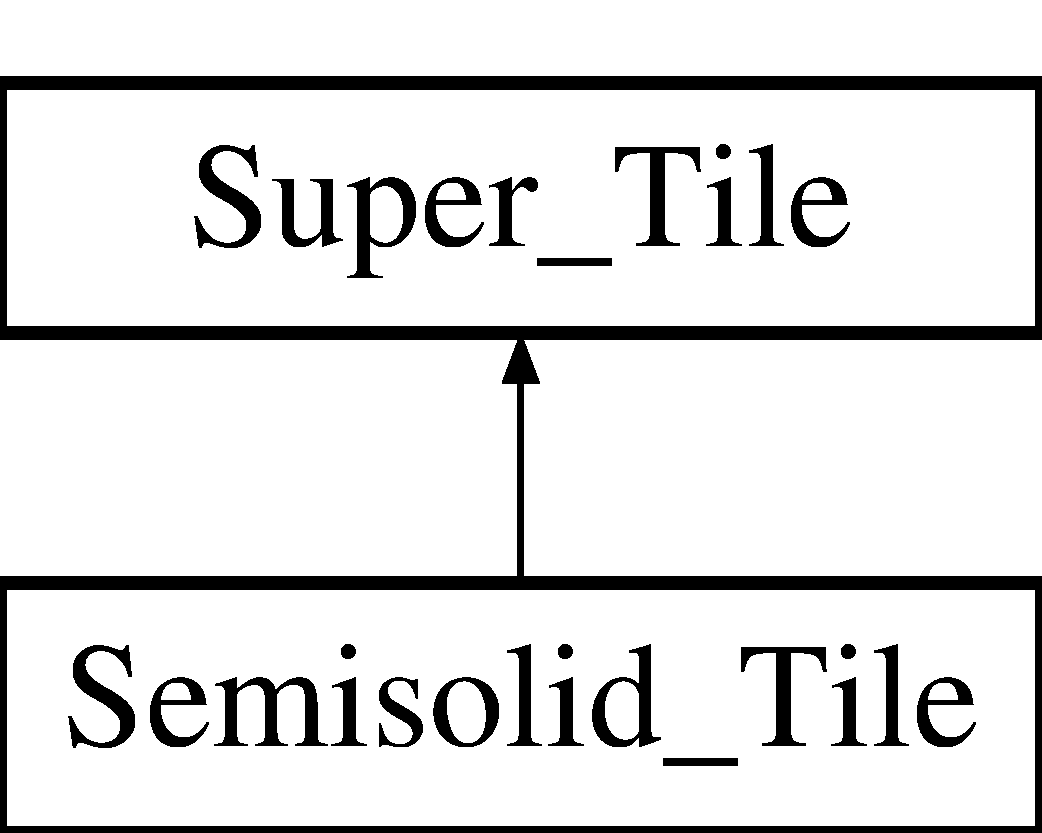
\includegraphics[height=2.000000cm]{class_semisolid___tile}
\end{center}
\end{figure}
\subsection*{Public Member Functions}
\begin{DoxyCompactItemize}
\item 
\hyperlink{class_semisolid___tile_a1fad2979b1c9d34e4311339f91e68149}{Semisolid\+\_\+\+Tile} (sf\+::\+Vector2f $\ast$\hyperlink{class_super___tile_ad6bcea1fd54f67808f54ba2aacd88596}{nw}, sf\+::\+Vector2f $\ast$\hyperlink{class_super___tile_a55f6d2860da36f13019bd4e0d18364ca}{ne}, sf\+::\+Vector2f $\ast$\hyperlink{class_super___tile_ab384b89a7a631b8b75c4d405c51a23e1}{se}, sf\+::\+Vector2f $\ast$\hyperlink{class_super___tile_abe9efe0c3d1ed440395225843435dfc8}{sw})
\item 
void \hyperlink{class_semisolid___tile_a65c8e43f414282be042b81c62fc63431}{impact} (\hyperlink{class_actor___class}{Actor\+\_\+\+Class} $\ast$actor)
\end{DoxyCompactItemize}
\subsection*{Additional Inherited Members}


\subsection{Detailed Description}


Definition at line 10 of file Semisolid\+\_\+\+Tile.\+h.



\subsection{Constructor \& Destructor Documentation}
\hypertarget{class_semisolid___tile_a1fad2979b1c9d34e4311339f91e68149}{}\label{class_semisolid___tile_a1fad2979b1c9d34e4311339f91e68149} 
\index{Semisolid\+\_\+\+Tile@{Semisolid\+\_\+\+Tile}!Semisolid\+\_\+\+Tile@{Semisolid\+\_\+\+Tile}}
\index{Semisolid\+\_\+\+Tile@{Semisolid\+\_\+\+Tile}!Semisolid\+\_\+\+Tile@{Semisolid\+\_\+\+Tile}}
\subsubsection{\texorpdfstring{Semisolid\+\_\+\+Tile()}{Semisolid\_Tile()}}
{\footnotesize\ttfamily Semisolid\+\_\+\+Tile\+::\+Semisolid\+\_\+\+Tile (\begin{DoxyParamCaption}\item[{sf\+::\+Vector2f $\ast$}]{nw,  }\item[{sf\+::\+Vector2f $\ast$}]{ne,  }\item[{sf\+::\+Vector2f $\ast$}]{se,  }\item[{sf\+::\+Vector2f $\ast$}]{sw }\end{DoxyParamCaption})}



Definition at line 6 of file Semisolid\+\_\+\+Tile.\+cpp.



\subsection{Member Function Documentation}
\hypertarget{class_semisolid___tile_a65c8e43f414282be042b81c62fc63431}{}\label{class_semisolid___tile_a65c8e43f414282be042b81c62fc63431} 
\index{Semisolid\+\_\+\+Tile@{Semisolid\+\_\+\+Tile}!impact@{impact}}
\index{impact@{impact}!Semisolid\+\_\+\+Tile@{Semisolid\+\_\+\+Tile}}
\subsubsection{\texorpdfstring{impact()}{impact()}}
{\footnotesize\ttfamily void Semisolid\+\_\+\+Tile\+::impact (\begin{DoxyParamCaption}\item[{\hyperlink{class_actor___class}{Actor\+\_\+\+Class} $\ast$}]{actor }\end{DoxyParamCaption})\hspace{0.3cm}{\ttfamily [inline]}, {\ttfamily [virtual]}}



Reimplemented from \hyperlink{class_super___tile_a7b509383d0d0ad2df0220f7dc4660823}{Super\+\_\+\+Tile}.



Definition at line 13 of file Semisolid\+\_\+\+Tile.\+h.



The documentation for this class was generated from the following files\+:\begin{DoxyCompactItemize}
\item 
Tile/\hyperlink{_semisolid___tile_8h}{Semisolid\+\_\+\+Tile.\+h}\item 
Tile/\hyperlink{_semisolid___tile_8cpp}{Semisolid\+\_\+\+Tile.\+cpp}\end{DoxyCompactItemize}

\hypertarget{class_settings___state}{}\section{Settings\+\_\+\+State Class Reference}
\label{class_settings___state}\index{Settings\+\_\+\+State@{Settings\+\_\+\+State}}


{\ttfamily \#include $<$settings\+\_\+state.\+h$>$}

Inheritance diagram for Settings\+\_\+\+State\+:\begin{figure}[H]
\begin{center}
\leavevmode
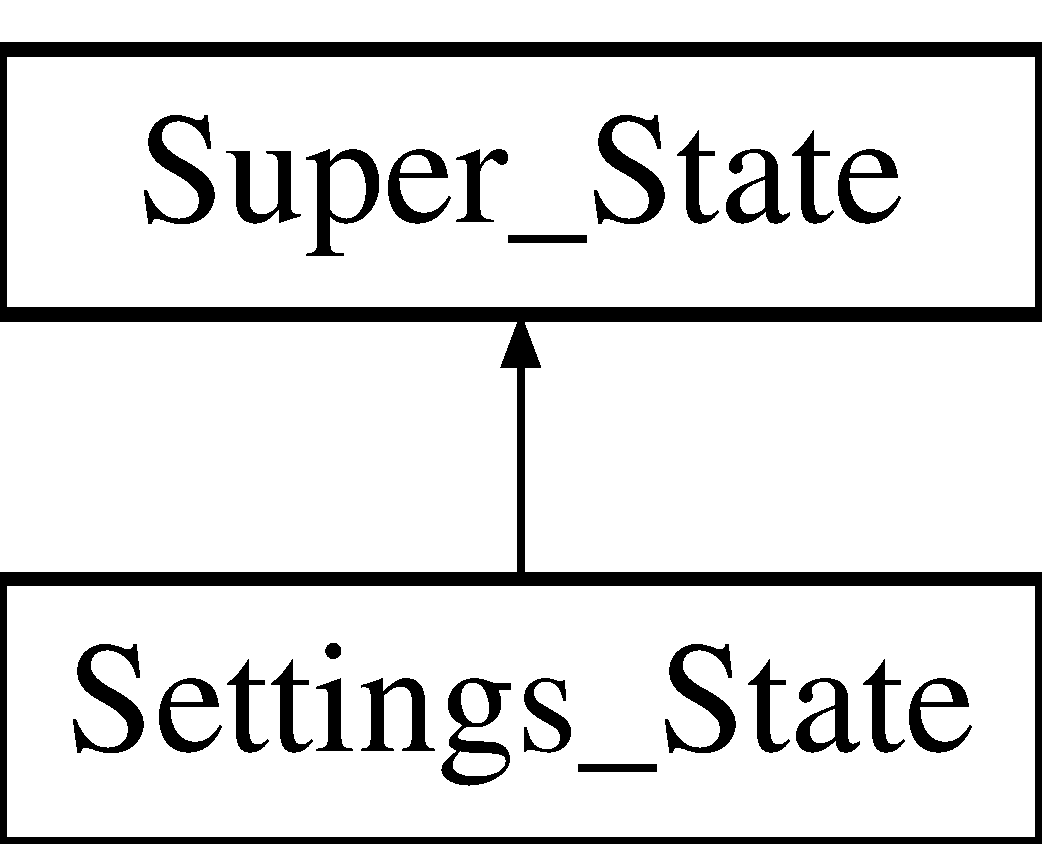
\includegraphics[height=2.000000cm]{class_settings___state}
\end{center}
\end{figure}
\subsection*{Public Member Functions}
\begin{DoxyCompactItemize}
\item 
\hyperlink{class_settings___state_a3b7db311952a3a13613e04a776d90ea5}{Settings\+\_\+\+State} (sf\+::\+Render\+Window \&\hyperlink{class_settings___state_ac560b251f0f6211bac46099994fa30eb}{window})
\item 
void \hyperlink{class_settings___state_a074aa49707b3a4fe530a105f274db1ae}{switch\+To} ()
\end{DoxyCompactItemize}
\subsection*{Public Attributes}
\begin{DoxyCompactItemize}
\item 
sf\+::\+Render\+Window \& \hyperlink{class_settings___state_ac560b251f0f6211bac46099994fa30eb}{window}
\end{DoxyCompactItemize}


\subsection{Detailed Description}


Definition at line 10 of file settings\+\_\+state.\+h.



\subsection{Constructor \& Destructor Documentation}
\hypertarget{class_settings___state_a3b7db311952a3a13613e04a776d90ea5}{}\label{class_settings___state_a3b7db311952a3a13613e04a776d90ea5} 
\index{Settings\+\_\+\+State@{Settings\+\_\+\+State}!Settings\+\_\+\+State@{Settings\+\_\+\+State}}
\index{Settings\+\_\+\+State@{Settings\+\_\+\+State}!Settings\+\_\+\+State@{Settings\+\_\+\+State}}
\subsubsection{\texorpdfstring{Settings\+\_\+\+State()}{Settings\_State()}}
{\footnotesize\ttfamily Settings\+\_\+\+State\+::\+Settings\+\_\+\+State (\begin{DoxyParamCaption}\item[{sf\+::\+Render\+Window \&}]{window }\end{DoxyParamCaption})}



Definition at line 9 of file settings\+\_\+state.\+cpp.



\subsection{Member Function Documentation}
\hypertarget{class_settings___state_a074aa49707b3a4fe530a105f274db1ae}{}\label{class_settings___state_a074aa49707b3a4fe530a105f274db1ae} 
\index{Settings\+\_\+\+State@{Settings\+\_\+\+State}!switch\+To@{switch\+To}}
\index{switch\+To@{switch\+To}!Settings\+\_\+\+State@{Settings\+\_\+\+State}}
\subsubsection{\texorpdfstring{switch\+To()}{switchTo()}}
{\footnotesize\ttfamily void Settings\+\_\+\+State\+::switch\+To (\begin{DoxyParamCaption}{ }\end{DoxyParamCaption})}



Definition at line 84 of file settings\+\_\+state.\+cpp.



\subsection{Member Data Documentation}
\hypertarget{class_settings___state_ac560b251f0f6211bac46099994fa30eb}{}\label{class_settings___state_ac560b251f0f6211bac46099994fa30eb} 
\index{Settings\+\_\+\+State@{Settings\+\_\+\+State}!window@{window}}
\index{window@{window}!Settings\+\_\+\+State@{Settings\+\_\+\+State}}
\subsubsection{\texorpdfstring{window}{window}}
{\footnotesize\ttfamily sf\+::\+Render\+Window\& Settings\+\_\+\+State\+::window}



Definition at line 16 of file settings\+\_\+state.\+h.



The documentation for this class was generated from the following files\+:\begin{DoxyCompactItemize}
\item 
States/\hyperlink{settings__state_8h}{settings\+\_\+state.\+h}\item 
States/\hyperlink{settings__state_8cpp}{settings\+\_\+state.\+cpp}\end{DoxyCompactItemize}

\hypertarget{class_shooting___mechanic}{}\section{Shooting\+\_\+\+Mechanic Class Reference}
\label{class_shooting___mechanic}\index{Shooting\+\_\+\+Mechanic@{Shooting\+\_\+\+Mechanic}}


{\ttfamily \#include $<$Shooting\+\_\+\+Mechanic.\+h$>$}

Inheritance diagram for Shooting\+\_\+\+Mechanic\+:\begin{figure}[H]
\begin{center}
\leavevmode
\includegraphics[height=2.000000cm]{class_shooting___mechanic}
\end{center}
\end{figure}
\subsection*{Public Member Functions}
\begin{DoxyCompactItemize}
\item 
\hyperlink{class_shooting___mechanic_a2c1defa547e5b53d057a5296d6776107}{Shooting\+\_\+\+Mechanic} (sf\+::\+Render\+Window \&window, \hyperlink{class_collision}{Collision} $\ast$col, \hyperlink{class_config}{Config} conf)
\item 
void \hyperlink{class_shooting___mechanic_a563bb47b2bb1c5f141cf47579d1402a6}{draw} ()
\item 
void \hyperlink{class_shooting___mechanic_a24b0992f715aa5e07a8d81c229401de0}{hero\+Shot} (\hyperlink{class_actor___class}{Actor\+\_\+\+Class} $\ast$helt, int kamera\+Pos)
\item 
void \hyperlink{class_shooting___mechanic_a2589f160241b7703aa04a3e2ffb11a9a}{enemyshot} (std\+::vector$<$ \hyperlink{class_actor___class}{Actor\+\_\+\+Class} $\ast$$>$ actor\+\_\+array, int kamera\+Pos)
\item 
void \hyperlink{class_shooting___mechanic_ae400341fd136cbd1ba39e5bcef2d6537}{erase\+Projectile} (int proj\+Index)
\end{DoxyCompactItemize}
\subsection*{Public Attributes}
\begin{DoxyCompactItemize}
\item 
\hyperlink{class_collision}{Collision} $\ast$ \hyperlink{class_shooting___mechanic_a73bdc235eb4ec579ba4d715cdb295e4e}{kollisjon}
\end{DoxyCompactItemize}
\subsection*{Protected Attributes}
\begin{DoxyCompactItemize}
\item 
\hyperlink{class_config}{Config} \hyperlink{class_shooting___mechanic_a69eb7f584def4225d9d0047f54489035}{configer}
\item 
int \hyperlink{class_shooting___mechanic_ac278fe303596d7b0f20e28ff8b4a8ed4}{dir} = 1
\item 
bool \hyperlink{class_shooting___mechanic_a7c7d3ab2cad3c1cecf5e167021960128}{key\+Pressed} = false
\item 
std\+::vector$<$ \hyperlink{class_projectile}{Projectile} $\ast$ $>$ \hyperlink{class_shooting___mechanic_a9fb5ad128dfb480bbb8174b07be01d92}{bullet\+Vector}
\item 
sf\+::\+Render\+Window \& \hyperlink{class_shooting___mechanic_a74fc67d9d6a2840ca3f2500b964cc3e4}{vindu}
\item 
\hyperlink{class_sound}{Sound} \hyperlink{class_shooting___mechanic_aae7e73612b2103509fb73b11f0a24b70}{sound}
\item 
\hyperlink{classanimatonsprites}{animatonsprites} \hyperlink{class_shooting___mechanic_af5bec55c10082be57809d48c1c83254c}{animasjon}
\end{DoxyCompactItemize}


\subsection{Detailed Description}


Definition at line 18 of file Shooting\+\_\+\+Mechanic.\+h.



\subsection{Constructor \& Destructor Documentation}
\hypertarget{class_shooting___mechanic_a2c1defa547e5b53d057a5296d6776107}{}\label{class_shooting___mechanic_a2c1defa547e5b53d057a5296d6776107} 
\index{Shooting\+\_\+\+Mechanic@{Shooting\+\_\+\+Mechanic}!Shooting\+\_\+\+Mechanic@{Shooting\+\_\+\+Mechanic}}
\index{Shooting\+\_\+\+Mechanic@{Shooting\+\_\+\+Mechanic}!Shooting\+\_\+\+Mechanic@{Shooting\+\_\+\+Mechanic}}
\subsubsection{\texorpdfstring{Shooting\+\_\+\+Mechanic()}{Shooting\_Mechanic()}}
{\footnotesize\ttfamily Shooting\+\_\+\+Mechanic\+::\+Shooting\+\_\+\+Mechanic (\begin{DoxyParamCaption}\item[{sf\+::\+Render\+Window \&}]{window,  }\item[{\hyperlink{class_collision}{Collision} $\ast$}]{col,  }\item[{\hyperlink{class_config}{Config}}]{conf }\end{DoxyParamCaption})}



Definition at line 7 of file Shooting\+\_\+\+Mechanic.\+cpp.



\subsection{Member Function Documentation}
\hypertarget{class_shooting___mechanic_a563bb47b2bb1c5f141cf47579d1402a6}{}\label{class_shooting___mechanic_a563bb47b2bb1c5f141cf47579d1402a6} 
\index{Shooting\+\_\+\+Mechanic@{Shooting\+\_\+\+Mechanic}!draw@{draw}}
\index{draw@{draw}!Shooting\+\_\+\+Mechanic@{Shooting\+\_\+\+Mechanic}}
\subsubsection{\texorpdfstring{draw()}{draw()}}
{\footnotesize\ttfamily void Shooting\+\_\+\+Mechanic\+::draw (\begin{DoxyParamCaption}{ }\end{DoxyParamCaption})}



Definition at line 181 of file Shooting\+\_\+\+Mechanic.\+cpp.

\hypertarget{class_shooting___mechanic_a2589f160241b7703aa04a3e2ffb11a9a}{}\label{class_shooting___mechanic_a2589f160241b7703aa04a3e2ffb11a9a} 
\index{Shooting\+\_\+\+Mechanic@{Shooting\+\_\+\+Mechanic}!enemyshot@{enemyshot}}
\index{enemyshot@{enemyshot}!Shooting\+\_\+\+Mechanic@{Shooting\+\_\+\+Mechanic}}
\subsubsection{\texorpdfstring{enemyshot()}{enemyshot()}}
{\footnotesize\ttfamily void Shooting\+\_\+\+Mechanic\+::enemyshot (\begin{DoxyParamCaption}\item[{std\+::vector$<$ \hyperlink{class_actor___class}{Actor\+\_\+\+Class} $\ast$$>$}]{actor\+\_\+array,  }\item[{int}]{kamera\+Pos }\end{DoxyParamCaption})}



Definition at line 70 of file Shooting\+\_\+\+Mechanic.\+cpp.

\hypertarget{class_shooting___mechanic_ae400341fd136cbd1ba39e5bcef2d6537}{}\label{class_shooting___mechanic_ae400341fd136cbd1ba39e5bcef2d6537} 
\index{Shooting\+\_\+\+Mechanic@{Shooting\+\_\+\+Mechanic}!erase\+Projectile@{erase\+Projectile}}
\index{erase\+Projectile@{erase\+Projectile}!Shooting\+\_\+\+Mechanic@{Shooting\+\_\+\+Mechanic}}
\subsubsection{\texorpdfstring{erase\+Projectile()}{eraseProjectile()}}
{\footnotesize\ttfamily void Shooting\+\_\+\+Mechanic\+::erase\+Projectile (\begin{DoxyParamCaption}\item[{int}]{proj\+Index }\end{DoxyParamCaption})}



Definition at line 177 of file Shooting\+\_\+\+Mechanic.\+cpp.

\hypertarget{class_shooting___mechanic_a24b0992f715aa5e07a8d81c229401de0}{}\label{class_shooting___mechanic_a24b0992f715aa5e07a8d81c229401de0} 
\index{Shooting\+\_\+\+Mechanic@{Shooting\+\_\+\+Mechanic}!hero\+Shot@{hero\+Shot}}
\index{hero\+Shot@{hero\+Shot}!Shooting\+\_\+\+Mechanic@{Shooting\+\_\+\+Mechanic}}
\subsubsection{\texorpdfstring{hero\+Shot()}{heroShot()}}
{\footnotesize\ttfamily void Shooting\+\_\+\+Mechanic\+::hero\+Shot (\begin{DoxyParamCaption}\item[{\hyperlink{class_actor___class}{Actor\+\_\+\+Class} $\ast$}]{helt,  }\item[{int}]{kamera\+Pos }\end{DoxyParamCaption})}

lagrer kule rettning 

Definition at line 15 of file Shooting\+\_\+\+Mechanic.\+cpp.



\subsection{Member Data Documentation}
\hypertarget{class_shooting___mechanic_af5bec55c10082be57809d48c1c83254c}{}\label{class_shooting___mechanic_af5bec55c10082be57809d48c1c83254c} 
\index{Shooting\+\_\+\+Mechanic@{Shooting\+\_\+\+Mechanic}!animasjon@{animasjon}}
\index{animasjon@{animasjon}!Shooting\+\_\+\+Mechanic@{Shooting\+\_\+\+Mechanic}}
\subsubsection{\texorpdfstring{animasjon}{animasjon}}
{\footnotesize\ttfamily \hyperlink{classanimatonsprites}{animatonsprites} Shooting\+\_\+\+Mechanic\+::animasjon\hspace{0.3cm}{\ttfamily [protected]}}



Definition at line 27 of file Shooting\+\_\+\+Mechanic.\+h.

\hypertarget{class_shooting___mechanic_a9fb5ad128dfb480bbb8174b07be01d92}{}\label{class_shooting___mechanic_a9fb5ad128dfb480bbb8174b07be01d92} 
\index{Shooting\+\_\+\+Mechanic@{Shooting\+\_\+\+Mechanic}!bullet\+Vector@{bullet\+Vector}}
\index{bullet\+Vector@{bullet\+Vector}!Shooting\+\_\+\+Mechanic@{Shooting\+\_\+\+Mechanic}}
\subsubsection{\texorpdfstring{bullet\+Vector}{bulletVector}}
{\footnotesize\ttfamily std\+::vector$<$\hyperlink{class_projectile}{Projectile}$\ast$$>$ Shooting\+\_\+\+Mechanic\+::bullet\+Vector\hspace{0.3cm}{\ttfamily [protected]}}



Definition at line 24 of file Shooting\+\_\+\+Mechanic.\+h.

\hypertarget{class_shooting___mechanic_a69eb7f584def4225d9d0047f54489035}{}\label{class_shooting___mechanic_a69eb7f584def4225d9d0047f54489035} 
\index{Shooting\+\_\+\+Mechanic@{Shooting\+\_\+\+Mechanic}!configer@{configer}}
\index{configer@{configer}!Shooting\+\_\+\+Mechanic@{Shooting\+\_\+\+Mechanic}}
\subsubsection{\texorpdfstring{configer}{configer}}
{\footnotesize\ttfamily \hyperlink{class_config}{Config} Shooting\+\_\+\+Mechanic\+::configer\hspace{0.3cm}{\ttfamily [protected]}}



Definition at line 21 of file Shooting\+\_\+\+Mechanic.\+h.

\hypertarget{class_shooting___mechanic_ac278fe303596d7b0f20e28ff8b4a8ed4}{}\label{class_shooting___mechanic_ac278fe303596d7b0f20e28ff8b4a8ed4} 
\index{Shooting\+\_\+\+Mechanic@{Shooting\+\_\+\+Mechanic}!dir@{dir}}
\index{dir@{dir}!Shooting\+\_\+\+Mechanic@{Shooting\+\_\+\+Mechanic}}
\subsubsection{\texorpdfstring{dir}{dir}}
{\footnotesize\ttfamily int Shooting\+\_\+\+Mechanic\+::dir = 1\hspace{0.3cm}{\ttfamily [protected]}}



Definition at line 22 of file Shooting\+\_\+\+Mechanic.\+h.

\hypertarget{class_shooting___mechanic_a7c7d3ab2cad3c1cecf5e167021960128}{}\label{class_shooting___mechanic_a7c7d3ab2cad3c1cecf5e167021960128} 
\index{Shooting\+\_\+\+Mechanic@{Shooting\+\_\+\+Mechanic}!key\+Pressed@{key\+Pressed}}
\index{key\+Pressed@{key\+Pressed}!Shooting\+\_\+\+Mechanic@{Shooting\+\_\+\+Mechanic}}
\subsubsection{\texorpdfstring{key\+Pressed}{keyPressed}}
{\footnotesize\ttfamily bool Shooting\+\_\+\+Mechanic\+::key\+Pressed = false\hspace{0.3cm}{\ttfamily [protected]}}



Definition at line 23 of file Shooting\+\_\+\+Mechanic.\+h.

\hypertarget{class_shooting___mechanic_a73bdc235eb4ec579ba4d715cdb295e4e}{}\label{class_shooting___mechanic_a73bdc235eb4ec579ba4d715cdb295e4e} 
\index{Shooting\+\_\+\+Mechanic@{Shooting\+\_\+\+Mechanic}!kollisjon@{kollisjon}}
\index{kollisjon@{kollisjon}!Shooting\+\_\+\+Mechanic@{Shooting\+\_\+\+Mechanic}}
\subsubsection{\texorpdfstring{kollisjon}{kollisjon}}
{\footnotesize\ttfamily \hyperlink{class_collision}{Collision}$\ast$ Shooting\+\_\+\+Mechanic\+::kollisjon}



Definition at line 36 of file Shooting\+\_\+\+Mechanic.\+h.

\hypertarget{class_shooting___mechanic_aae7e73612b2103509fb73b11f0a24b70}{}\label{class_shooting___mechanic_aae7e73612b2103509fb73b11f0a24b70} 
\index{Shooting\+\_\+\+Mechanic@{Shooting\+\_\+\+Mechanic}!sound@{sound}}
\index{sound@{sound}!Shooting\+\_\+\+Mechanic@{Shooting\+\_\+\+Mechanic}}
\subsubsection{\texorpdfstring{sound}{sound}}
{\footnotesize\ttfamily \hyperlink{class_sound}{Sound} Shooting\+\_\+\+Mechanic\+::sound\hspace{0.3cm}{\ttfamily [protected]}}



Definition at line 26 of file Shooting\+\_\+\+Mechanic.\+h.

\hypertarget{class_shooting___mechanic_a74fc67d9d6a2840ca3f2500b964cc3e4}{}\label{class_shooting___mechanic_a74fc67d9d6a2840ca3f2500b964cc3e4} 
\index{Shooting\+\_\+\+Mechanic@{Shooting\+\_\+\+Mechanic}!vindu@{vindu}}
\index{vindu@{vindu}!Shooting\+\_\+\+Mechanic@{Shooting\+\_\+\+Mechanic}}
\subsubsection{\texorpdfstring{vindu}{vindu}}
{\footnotesize\ttfamily sf\+::\+Render\+Window\& Shooting\+\_\+\+Mechanic\+::vindu\hspace{0.3cm}{\ttfamily [protected]}}



Definition at line 25 of file Shooting\+\_\+\+Mechanic.\+h.



The documentation for this class was generated from the following files\+:\begin{DoxyCompactItemize}
\item 
Actor/projectil/\hyperlink{_shooting___mechanic_8h}{Shooting\+\_\+\+Mechanic.\+h}\item 
Actor/projectil/\hyperlink{_shooting___mechanic_8cpp}{Shooting\+\_\+\+Mechanic.\+cpp}\end{DoxyCompactItemize}

\hypertarget{class_solid___tile}{}\section{Solid\+\_\+\+Tile Class Reference}
\label{class_solid___tile}\index{Solid\+\_\+\+Tile@{Solid\+\_\+\+Tile}}


{\ttfamily \#include $<$Solid\+\_\+\+Tile.\+h$>$}

Inheritance diagram for Solid\+\_\+\+Tile\+:\begin{figure}[H]
\begin{center}
\leavevmode
\includegraphics[height=2.000000cm]{class_solid___tile}
\end{center}
\end{figure}
\subsection*{Public Member Functions}
\begin{DoxyCompactItemize}
\item 
\hyperlink{class_solid___tile_a2f40382f46c06ba040266d2b37503101}{Solid\+\_\+\+Tile} (sf\+::\+Vector2f $\ast$\hyperlink{class_super___tile_ad6bcea1fd54f67808f54ba2aacd88596}{nw}, sf\+::\+Vector2f $\ast$\hyperlink{class_super___tile_a55f6d2860da36f13019bd4e0d18364ca}{ne}, sf\+::\+Vector2f $\ast$\hyperlink{class_super___tile_ab384b89a7a631b8b75c4d405c51a23e1}{se}, sf\+::\+Vector2f $\ast$\hyperlink{class_super___tile_abe9efe0c3d1ed440395225843435dfc8}{sw})
\item 
void \hyperlink{class_solid___tile_ada34ec00762b7df804292f40fbeecc95}{impact} (\hyperlink{class_actor___class}{Actor\+\_\+\+Class} $\ast$actor)
\end{DoxyCompactItemize}
\subsection*{Additional Inherited Members}


\subsection{Detailed Description}


Definition at line 10 of file Solid\+\_\+\+Tile.\+h.



\subsection{Constructor \& Destructor Documentation}
\hypertarget{class_solid___tile_a2f40382f46c06ba040266d2b37503101}{}\label{class_solid___tile_a2f40382f46c06ba040266d2b37503101} 
\index{Solid\+\_\+\+Tile@{Solid\+\_\+\+Tile}!Solid\+\_\+\+Tile@{Solid\+\_\+\+Tile}}
\index{Solid\+\_\+\+Tile@{Solid\+\_\+\+Tile}!Solid\+\_\+\+Tile@{Solid\+\_\+\+Tile}}
\subsubsection{\texorpdfstring{Solid\+\_\+\+Tile()}{Solid\_Tile()}}
{\footnotesize\ttfamily Solid\+\_\+\+Tile\+::\+Solid\+\_\+\+Tile (\begin{DoxyParamCaption}\item[{sf\+::\+Vector2f $\ast$}]{nw,  }\item[{sf\+::\+Vector2f $\ast$}]{ne,  }\item[{sf\+::\+Vector2f $\ast$}]{se,  }\item[{sf\+::\+Vector2f $\ast$}]{sw }\end{DoxyParamCaption})}



Definition at line 8 of file Solid\+\_\+\+Tile.\+cpp.



\subsection{Member Function Documentation}
\hypertarget{class_solid___tile_ada34ec00762b7df804292f40fbeecc95}{}\label{class_solid___tile_ada34ec00762b7df804292f40fbeecc95} 
\index{Solid\+\_\+\+Tile@{Solid\+\_\+\+Tile}!impact@{impact}}
\index{impact@{impact}!Solid\+\_\+\+Tile@{Solid\+\_\+\+Tile}}
\subsubsection{\texorpdfstring{impact()}{impact()}}
{\footnotesize\ttfamily void Solid\+\_\+\+Tile\+::impact (\begin{DoxyParamCaption}\item[{\hyperlink{class_actor___class}{Actor\+\_\+\+Class} $\ast$}]{actor }\end{DoxyParamCaption})\hspace{0.3cm}{\ttfamily [virtual]}}



Reimplemented from \hyperlink{class_super___tile_a7b509383d0d0ad2df0220f7dc4660823}{Super\+\_\+\+Tile}.



Definition at line 15 of file Solid\+\_\+\+Tile.\+cpp.



The documentation for this class was generated from the following files\+:\begin{DoxyCompactItemize}
\item 
Tile/\hyperlink{_solid___tile_8h}{Solid\+\_\+\+Tile.\+h}\item 
Tile/\hyperlink{_solid___tile_8cpp}{Solid\+\_\+\+Tile.\+cpp}\end{DoxyCompactItemize}

\hypertarget{class_sound}{}\section{Sound Class Reference}
\label{class_sound}\index{Sound@{Sound}}


{\ttfamily \#include $<$Sound.\+h$>$}

\subsection*{Public Member Functions}
\begin{DoxyCompactItemize}
\item 
\hyperlink{class_sound_a539c205cdf06fe2c621fd77c37bcfac9}{Sound} ()
\item 
void \hyperlink{class_sound_a696d9a188670c54d240fce5c43ced879}{play\+Jump} ()
\begin{DoxyCompactList}\small\item\em play jump sound \end{DoxyCompactList}\item 
void \hyperlink{class_sound_a4cb3a0ff7fb89b3267cc1d0e7abec829}{play\+Shoot} ()
\begin{DoxyCompactList}\small\item\em play shoot sound \end{DoxyCompactList}\item 
void \hyperlink{class_sound_a8745b80c3bdd62893f74383cb939ca6e}{play\+Hit} ()
\item 
void \hyperlink{class_sound_a56de021d1ec151a13e4e9f8b583eef24}{play\+Hit\+Enemy} ()
\end{DoxyCompactItemize}
\subsection*{Public Attributes}
\begin{DoxyCompactItemize}
\item 
sf\+::\+Sound \hyperlink{class_sound_a49188be0a133d32388a600764aee8959}{jump}
\item 
sf\+::\+Sound \hyperlink{class_sound_abe6dfe8e86c4fa694b0d5ce693213f2f}{shoot}
\item 
sf\+::\+Sound \hyperlink{class_sound_a8fdfa5eda5eff47c878e245c816cf4d9}{hit}
\item 
sf\+::\+Sound \hyperlink{class_sound_aca883eb04a7aa8844095afd7d397976a}{hit\+Enemy}
\item 
sf\+::\+Sound\+Buffer \hyperlink{class_sound_afb04ee141c3765d1cd14fef2268029f3}{jump\+Buffer}
\item 
sf\+::\+Sound\+Buffer \hyperlink{class_sound_a963c0081728c14318b99dc8618a950c6}{shoot\+Buffer}
\item 
sf\+::\+Sound\+Buffer \hyperlink{class_sound_ad68e36ce916f5b858aaf467a6fd929e1}{hit\+Buffer}
\item 
sf\+::\+Sound\+Buffer \hyperlink{class_sound_a5a2a2ccabe0099ebf4c8fc3cbb8edff6}{hit\+Enemy\+Buffer}
\end{DoxyCompactItemize}


\subsection{Detailed Description}


Definition at line 10 of file Sound.\+h.



\subsection{Constructor \& Destructor Documentation}
\hypertarget{class_sound_a539c205cdf06fe2c621fd77c37bcfac9}{}\label{class_sound_a539c205cdf06fe2c621fd77c37bcfac9} 
\index{Sound@{Sound}!Sound@{Sound}}
\index{Sound@{Sound}!Sound@{Sound}}
\subsubsection{\texorpdfstring{Sound()}{Sound()}}
{\footnotesize\ttfamily Sound\+::\+Sound (\begin{DoxyParamCaption}{ }\end{DoxyParamCaption})}

load sounds \begin{DoxyReturn}{Returns}

\end{DoxyReturn}


Definition at line 6 of file Sound.\+cpp.



\subsection{Member Function Documentation}
\hypertarget{class_sound_a8745b80c3bdd62893f74383cb939ca6e}{}\label{class_sound_a8745b80c3bdd62893f74383cb939ca6e} 
\index{Sound@{Sound}!play\+Hit@{play\+Hit}}
\index{play\+Hit@{play\+Hit}!Sound@{Sound}}
\subsubsection{\texorpdfstring{play\+Hit()}{playHit()}}
{\footnotesize\ttfamily void Sound\+::play\+Hit (\begin{DoxyParamCaption}{ }\end{DoxyParamCaption})}



Definition at line 28 of file Sound.\+cpp.

\hypertarget{class_sound_a56de021d1ec151a13e4e9f8b583eef24}{}\label{class_sound_a56de021d1ec151a13e4e9f8b583eef24} 
\index{Sound@{Sound}!play\+Hit\+Enemy@{play\+Hit\+Enemy}}
\index{play\+Hit\+Enemy@{play\+Hit\+Enemy}!Sound@{Sound}}
\subsubsection{\texorpdfstring{play\+Hit\+Enemy()}{playHitEnemy()}}
{\footnotesize\ttfamily void Sound\+::play\+Hit\+Enemy (\begin{DoxyParamCaption}{ }\end{DoxyParamCaption})}



Definition at line 33 of file Sound.\+cpp.

\hypertarget{class_sound_a696d9a188670c54d240fce5c43ced879}{}\label{class_sound_a696d9a188670c54d240fce5c43ced879} 
\index{Sound@{Sound}!play\+Jump@{play\+Jump}}
\index{play\+Jump@{play\+Jump}!Sound@{Sound}}
\subsubsection{\texorpdfstring{play\+Jump()}{playJump()}}
{\footnotesize\ttfamily void Sound\+::play\+Jump (\begin{DoxyParamCaption}{ }\end{DoxyParamCaption})}



play jump sound 



Definition at line 23 of file Sound.\+cpp.

\hypertarget{class_sound_a4cb3a0ff7fb89b3267cc1d0e7abec829}{}\label{class_sound_a4cb3a0ff7fb89b3267cc1d0e7abec829} 
\index{Sound@{Sound}!play\+Shoot@{play\+Shoot}}
\index{play\+Shoot@{play\+Shoot}!Sound@{Sound}}
\subsubsection{\texorpdfstring{play\+Shoot()}{playShoot()}}
{\footnotesize\ttfamily void Sound\+::play\+Shoot (\begin{DoxyParamCaption}{ }\end{DoxyParamCaption})}



play shoot sound 



Definition at line 18 of file Sound.\+cpp.



\subsection{Member Data Documentation}
\hypertarget{class_sound_a8fdfa5eda5eff47c878e245c816cf4d9}{}\label{class_sound_a8fdfa5eda5eff47c878e245c816cf4d9} 
\index{Sound@{Sound}!hit@{hit}}
\index{hit@{hit}!Sound@{Sound}}
\subsubsection{\texorpdfstring{hit}{hit}}
{\footnotesize\ttfamily sf\+::\+Sound Sound\+::hit}



Definition at line 26 of file Sound.\+h.

\hypertarget{class_sound_ad68e36ce916f5b858aaf467a6fd929e1}{}\label{class_sound_ad68e36ce916f5b858aaf467a6fd929e1} 
\index{Sound@{Sound}!hit\+Buffer@{hit\+Buffer}}
\index{hit\+Buffer@{hit\+Buffer}!Sound@{Sound}}
\subsubsection{\texorpdfstring{hit\+Buffer}{hitBuffer}}
{\footnotesize\ttfamily sf\+::\+Sound\+Buffer Sound\+::hit\+Buffer}



Definition at line 30 of file Sound.\+h.

\hypertarget{class_sound_aca883eb04a7aa8844095afd7d397976a}{}\label{class_sound_aca883eb04a7aa8844095afd7d397976a} 
\index{Sound@{Sound}!hit\+Enemy@{hit\+Enemy}}
\index{hit\+Enemy@{hit\+Enemy}!Sound@{Sound}}
\subsubsection{\texorpdfstring{hit\+Enemy}{hitEnemy}}
{\footnotesize\ttfamily sf\+::\+Sound Sound\+::hit\+Enemy}



Definition at line 27 of file Sound.\+h.

\hypertarget{class_sound_a5a2a2ccabe0099ebf4c8fc3cbb8edff6}{}\label{class_sound_a5a2a2ccabe0099ebf4c8fc3cbb8edff6} 
\index{Sound@{Sound}!hit\+Enemy\+Buffer@{hit\+Enemy\+Buffer}}
\index{hit\+Enemy\+Buffer@{hit\+Enemy\+Buffer}!Sound@{Sound}}
\subsubsection{\texorpdfstring{hit\+Enemy\+Buffer}{hitEnemyBuffer}}
{\footnotesize\ttfamily sf\+::\+Sound\+Buffer Sound\+::hit\+Enemy\+Buffer}



Definition at line 31 of file Sound.\+h.

\hypertarget{class_sound_a49188be0a133d32388a600764aee8959}{}\label{class_sound_a49188be0a133d32388a600764aee8959} 
\index{Sound@{Sound}!jump@{jump}}
\index{jump@{jump}!Sound@{Sound}}
\subsubsection{\texorpdfstring{jump}{jump}}
{\footnotesize\ttfamily sf\+::\+Sound Sound\+::jump}



Definition at line 24 of file Sound.\+h.

\hypertarget{class_sound_afb04ee141c3765d1cd14fef2268029f3}{}\label{class_sound_afb04ee141c3765d1cd14fef2268029f3} 
\index{Sound@{Sound}!jump\+Buffer@{jump\+Buffer}}
\index{jump\+Buffer@{jump\+Buffer}!Sound@{Sound}}
\subsubsection{\texorpdfstring{jump\+Buffer}{jumpBuffer}}
{\footnotesize\ttfamily sf\+::\+Sound\+Buffer Sound\+::jump\+Buffer}



Definition at line 28 of file Sound.\+h.

\hypertarget{class_sound_abe6dfe8e86c4fa694b0d5ce693213f2f}{}\label{class_sound_abe6dfe8e86c4fa694b0d5ce693213f2f} 
\index{Sound@{Sound}!shoot@{shoot}}
\index{shoot@{shoot}!Sound@{Sound}}
\subsubsection{\texorpdfstring{shoot}{shoot}}
{\footnotesize\ttfamily sf\+::\+Sound Sound\+::shoot}



Definition at line 25 of file Sound.\+h.

\hypertarget{class_sound_a963c0081728c14318b99dc8618a950c6}{}\label{class_sound_a963c0081728c14318b99dc8618a950c6} 
\index{Sound@{Sound}!shoot\+Buffer@{shoot\+Buffer}}
\index{shoot\+Buffer@{shoot\+Buffer}!Sound@{Sound}}
\subsubsection{\texorpdfstring{shoot\+Buffer}{shootBuffer}}
{\footnotesize\ttfamily sf\+::\+Sound\+Buffer Sound\+::shoot\+Buffer}



Definition at line 29 of file Sound.\+h.



The documentation for this class was generated from the following files\+:\begin{DoxyCompactItemize}
\item 
\hyperlink{_sound_8h}{Sound.\+h}\item 
\hyperlink{_sound_8cpp}{Sound.\+cpp}\end{DoxyCompactItemize}

\hypertarget{class_spawn___tile}{}\section{Spawn\+\_\+\+Tile Class Reference}
\label{class_spawn___tile}\index{Spawn\+\_\+\+Tile@{Spawn\+\_\+\+Tile}}


{\ttfamily \#include $<$Spawn\+\_\+\+Tile.\+h$>$}

Inheritance diagram for Spawn\+\_\+\+Tile\+:\begin{figure}[H]
\begin{center}
\leavevmode
\includegraphics[height=2.000000cm]{class_spawn___tile}
\end{center}
\end{figure}
\subsection*{Public Member Functions}
\begin{DoxyCompactItemize}
\item 
\hyperlink{class_spawn___tile_a9491bac6cc501fb9f0febde42533fc1d}{Spawn\+\_\+\+Tile} (sf\+::\+Vector2f $\ast$\hyperlink{class_super___tile_ad6bcea1fd54f67808f54ba2aacd88596}{nw}, sf\+::\+Vector2f $\ast$\hyperlink{class_super___tile_a55f6d2860da36f13019bd4e0d18364ca}{ne}, sf\+::\+Vector2f $\ast$\hyperlink{class_super___tile_ab384b89a7a631b8b75c4d405c51a23e1}{se}, sf\+::\+Vector2f $\ast$\hyperlink{class_super___tile_abe9efe0c3d1ed440395225843435dfc8}{sw}, int spawn\+Actor)
\item 
void \hyperlink{class_spawn___tile_a9b557377a8afd06512ac19368a4f14a4}{impact} (\hyperlink{class_actor___class}{Actor\+\_\+\+Class} $\ast$actor)
\item 
int \hyperlink{class_spawn___tile_a97168cfea2f8de79a6342c4b46d7eaf8}{spawn} ()
\end{DoxyCompactItemize}
\subsection*{Public Attributes}
\begin{DoxyCompactItemize}
\item 
int \hyperlink{class_spawn___tile_a43dfdce45bb37685e75666e3ec7331d1}{spawning\+Enemy\+Type}
\item 
bool \hyperlink{class_spawn___tile_a3007d9023153c7b33a16398f4de74dc7}{spawn\+Test}
\end{DoxyCompactItemize}


\subsection{Detailed Description}


Definition at line 10 of file Spawn\+\_\+\+Tile.\+h.



\subsection{Constructor \& Destructor Documentation}
\hypertarget{class_spawn___tile_a9491bac6cc501fb9f0febde42533fc1d}{}\label{class_spawn___tile_a9491bac6cc501fb9f0febde42533fc1d} 
\index{Spawn\+\_\+\+Tile@{Spawn\+\_\+\+Tile}!Spawn\+\_\+\+Tile@{Spawn\+\_\+\+Tile}}
\index{Spawn\+\_\+\+Tile@{Spawn\+\_\+\+Tile}!Spawn\+\_\+\+Tile@{Spawn\+\_\+\+Tile}}
\subsubsection{\texorpdfstring{Spawn\+\_\+\+Tile()}{Spawn\_Tile()}}
{\footnotesize\ttfamily Spawn\+\_\+\+Tile\+::\+Spawn\+\_\+\+Tile (\begin{DoxyParamCaption}\item[{sf\+::\+Vector2f $\ast$}]{nw,  }\item[{sf\+::\+Vector2f $\ast$}]{ne,  }\item[{sf\+::\+Vector2f $\ast$}]{se,  }\item[{sf\+::\+Vector2f $\ast$}]{sw,  }\item[{int}]{spawn\+Actor }\end{DoxyParamCaption})}



Definition at line 8 of file Spawn\+\_\+\+Tile.\+cpp.



\subsection{Member Function Documentation}
\hypertarget{class_spawn___tile_a9b557377a8afd06512ac19368a4f14a4}{}\label{class_spawn___tile_a9b557377a8afd06512ac19368a4f14a4} 
\index{Spawn\+\_\+\+Tile@{Spawn\+\_\+\+Tile}!impact@{impact}}
\index{impact@{impact}!Spawn\+\_\+\+Tile@{Spawn\+\_\+\+Tile}}
\subsubsection{\texorpdfstring{impact()}{impact()}}
{\footnotesize\ttfamily void Spawn\+\_\+\+Tile\+::impact (\begin{DoxyParamCaption}\item[{\hyperlink{class_actor___class}{Actor\+\_\+\+Class} $\ast$}]{actor }\end{DoxyParamCaption})\hspace{0.3cm}{\ttfamily [virtual]}}



Reimplemented from \hyperlink{class_super___tile_a7b509383d0d0ad2df0220f7dc4660823}{Super\+\_\+\+Tile}.



Definition at line 17 of file Spawn\+\_\+\+Tile.\+cpp.

\hypertarget{class_spawn___tile_a97168cfea2f8de79a6342c4b46d7eaf8}{}\label{class_spawn___tile_a97168cfea2f8de79a6342c4b46d7eaf8} 
\index{Spawn\+\_\+\+Tile@{Spawn\+\_\+\+Tile}!spawn@{spawn}}
\index{spawn@{spawn}!Spawn\+\_\+\+Tile@{Spawn\+\_\+\+Tile}}
\subsubsection{\texorpdfstring{spawn()}{spawn()}}
{\footnotesize\ttfamily int Spawn\+\_\+\+Tile\+::spawn (\begin{DoxyParamCaption}{ }\end{DoxyParamCaption})}



Definition at line 20 of file Spawn\+\_\+\+Tile.\+cpp.



\subsection{Member Data Documentation}
\hypertarget{class_spawn___tile_a43dfdce45bb37685e75666e3ec7331d1}{}\label{class_spawn___tile_a43dfdce45bb37685e75666e3ec7331d1} 
\index{Spawn\+\_\+\+Tile@{Spawn\+\_\+\+Tile}!spawning\+Enemy\+Type@{spawning\+Enemy\+Type}}
\index{spawning\+Enemy\+Type@{spawning\+Enemy\+Type}!Spawn\+\_\+\+Tile@{Spawn\+\_\+\+Tile}}
\subsubsection{\texorpdfstring{spawning\+Enemy\+Type}{spawningEnemyType}}
{\footnotesize\ttfamily int Spawn\+\_\+\+Tile\+::spawning\+Enemy\+Type}



Definition at line 13 of file Spawn\+\_\+\+Tile.\+h.

\hypertarget{class_spawn___tile_a3007d9023153c7b33a16398f4de74dc7}{}\label{class_spawn___tile_a3007d9023153c7b33a16398f4de74dc7} 
\index{Spawn\+\_\+\+Tile@{Spawn\+\_\+\+Tile}!spawn\+Test@{spawn\+Test}}
\index{spawn\+Test@{spawn\+Test}!Spawn\+\_\+\+Tile@{Spawn\+\_\+\+Tile}}
\subsubsection{\texorpdfstring{spawn\+Test}{spawnTest}}
{\footnotesize\ttfamily bool Spawn\+\_\+\+Tile\+::spawn\+Test}



Definition at line 14 of file Spawn\+\_\+\+Tile.\+h.



The documentation for this class was generated from the following files\+:\begin{DoxyCompactItemize}
\item 
Tile/action\+\_\+tile/\hyperlink{_spawn___tile_8h}{Spawn\+\_\+\+Tile.\+h}\item 
Tile/action\+\_\+tile/\hyperlink{_spawn___tile_8cpp}{Spawn\+\_\+\+Tile.\+cpp}\end{DoxyCompactItemize}

\hypertarget{class_speed___tile}{}\section{Speed\+\_\+\+Tile Class Reference}
\label{class_speed___tile}\index{Speed\+\_\+\+Tile@{Speed\+\_\+\+Tile}}


{\ttfamily \#include $<$Speed\+\_\+\+Tile.\+h$>$}

Inheritance diagram for Speed\+\_\+\+Tile\+:\begin{figure}[H]
\begin{center}
\leavevmode
\includegraphics[height=3.000000cm]{class_speed___tile}
\end{center}
\end{figure}
\subsection*{Public Member Functions}
\begin{DoxyCompactItemize}
\item 
\hyperlink{class_speed___tile_a296bb700865d7f78df9cdd830102aafd}{Speed\+\_\+\+Tile} (sf\+::\+Vector2f $\ast$\hyperlink{class_super___tile_ad6bcea1fd54f67808f54ba2aacd88596}{nw}, sf\+::\+Vector2f $\ast$\hyperlink{class_super___tile_a55f6d2860da36f13019bd4e0d18364ca}{ne}, sf\+::\+Vector2f $\ast$\hyperlink{class_super___tile_ab384b89a7a631b8b75c4d405c51a23e1}{se}, sf\+::\+Vector2f $\ast$\hyperlink{class_super___tile_abe9efe0c3d1ed440395225843435dfc8}{sw})
\item 
void \hyperlink{class_speed___tile_aea424ba028f29398ace251a3a664b874}{impact} (\hyperlink{class_actor___class}{Actor\+\_\+\+Class} $\ast$actor)
\end{DoxyCompactItemize}
\subsection*{Public Attributes}
\begin{DoxyCompactItemize}
\item 
int \hyperlink{class_speed___tile_af973cfe789cf50b9622db1fda43efd3c}{speed} = 3
\end{DoxyCompactItemize}


\subsection{Detailed Description}


Definition at line 9 of file Speed\+\_\+\+Tile.\+h.



\subsection{Constructor \& Destructor Documentation}
\hypertarget{class_speed___tile_a296bb700865d7f78df9cdd830102aafd}{}\label{class_speed___tile_a296bb700865d7f78df9cdd830102aafd} 
\index{Speed\+\_\+\+Tile@{Speed\+\_\+\+Tile}!Speed\+\_\+\+Tile@{Speed\+\_\+\+Tile}}
\index{Speed\+\_\+\+Tile@{Speed\+\_\+\+Tile}!Speed\+\_\+\+Tile@{Speed\+\_\+\+Tile}}
\subsubsection{\texorpdfstring{Speed\+\_\+\+Tile()}{Speed\_Tile()}}
{\footnotesize\ttfamily Speed\+\_\+\+Tile\+::\+Speed\+\_\+\+Tile (\begin{DoxyParamCaption}\item[{sf\+::\+Vector2f $\ast$}]{nw,  }\item[{sf\+::\+Vector2f $\ast$}]{ne,  }\item[{sf\+::\+Vector2f $\ast$}]{se,  }\item[{sf\+::\+Vector2f $\ast$}]{sw }\end{DoxyParamCaption})}



Definition at line 7 of file Speed\+\_\+\+Tile.\+cpp.



\subsection{Member Function Documentation}
\hypertarget{class_speed___tile_aea424ba028f29398ace251a3a664b874}{}\label{class_speed___tile_aea424ba028f29398ace251a3a664b874} 
\index{Speed\+\_\+\+Tile@{Speed\+\_\+\+Tile}!impact@{impact}}
\index{impact@{impact}!Speed\+\_\+\+Tile@{Speed\+\_\+\+Tile}}
\subsubsection{\texorpdfstring{impact()}{impact()}}
{\footnotesize\ttfamily void Speed\+\_\+\+Tile\+::impact (\begin{DoxyParamCaption}\item[{\hyperlink{class_actor___class}{Actor\+\_\+\+Class} $\ast$}]{actor }\end{DoxyParamCaption})\hspace{0.3cm}{\ttfamily [virtual]}}



Reimplemented from \hyperlink{class_action___tile_aa366fba2ea9d3947c28c45f939ee0217}{Action\+\_\+\+Tile}.



Definition at line 14 of file Speed\+\_\+\+Tile.\+cpp.



\subsection{Member Data Documentation}
\hypertarget{class_speed___tile_af973cfe789cf50b9622db1fda43efd3c}{}\label{class_speed___tile_af973cfe789cf50b9622db1fda43efd3c} 
\index{Speed\+\_\+\+Tile@{Speed\+\_\+\+Tile}!speed@{speed}}
\index{speed@{speed}!Speed\+\_\+\+Tile@{Speed\+\_\+\+Tile}}
\subsubsection{\texorpdfstring{speed}{speed}}
{\footnotesize\ttfamily int Speed\+\_\+\+Tile\+::speed = 3}



Definition at line 14 of file Speed\+\_\+\+Tile.\+h.



The documentation for this class was generated from the following files\+:\begin{DoxyCompactItemize}
\item 
Tile/action\+\_\+tile/\hyperlink{_speed___tile_8h}{Speed\+\_\+\+Tile.\+h}\item 
Tile/action\+\_\+tile/\hyperlink{_speed___tile_8cpp}{Speed\+\_\+\+Tile.\+cpp}\end{DoxyCompactItemize}

\hypertarget{class_spike___tile}{}\section{Spike\+\_\+\+Tile Class Reference}
\label{class_spike___tile}\index{Spike\+\_\+\+Tile@{Spike\+\_\+\+Tile}}


{\ttfamily \#include $<$Spike\+\_\+\+Tile.\+h$>$}

Inheritance diagram for Spike\+\_\+\+Tile\+:\begin{figure}[H]
\begin{center}
\leavevmode
\includegraphics[height=3.000000cm]{class_spike___tile}
\end{center}
\end{figure}
\subsection*{Public Member Functions}
\begin{DoxyCompactItemize}
\item 
\hyperlink{class_spike___tile_a7752370ac92d839421a0405965fec127}{Spike\+\_\+\+Tile} (sf\+::\+Vector2f $\ast$\hyperlink{class_super___tile_ad6bcea1fd54f67808f54ba2aacd88596}{nw}, sf\+::\+Vector2f $\ast$\hyperlink{class_super___tile_a55f6d2860da36f13019bd4e0d18364ca}{ne}, sf\+::\+Vector2f $\ast$\hyperlink{class_super___tile_ab384b89a7a631b8b75c4d405c51a23e1}{se}, sf\+::\+Vector2f $\ast$\hyperlink{class_super___tile_abe9efe0c3d1ed440395225843435dfc8}{sw})
\item 
void \hyperlink{class_spike___tile_a8673c82f84733fe73c456eee725a6ab0}{impact} (\hyperlink{class_actor___class}{Actor\+\_\+\+Class} $\ast$actor)
\end{DoxyCompactItemize}
\subsection*{Public Attributes}
\begin{DoxyCompactItemize}
\item 
int \hyperlink{class_spike___tile_af294383b8e83dfd6cfbc72b73174f8df}{leeway} = 14
\end{DoxyCompactItemize}


\subsection{Detailed Description}


Definition at line 11 of file Spike\+\_\+\+Tile.\+h.



\subsection{Constructor \& Destructor Documentation}
\hypertarget{class_spike___tile_a7752370ac92d839421a0405965fec127}{}\label{class_spike___tile_a7752370ac92d839421a0405965fec127} 
\index{Spike\+\_\+\+Tile@{Spike\+\_\+\+Tile}!Spike\+\_\+\+Tile@{Spike\+\_\+\+Tile}}
\index{Spike\+\_\+\+Tile@{Spike\+\_\+\+Tile}!Spike\+\_\+\+Tile@{Spike\+\_\+\+Tile}}
\subsubsection{\texorpdfstring{Spike\+\_\+\+Tile()}{Spike\_Tile()}}
{\footnotesize\ttfamily Spike\+\_\+\+Tile\+::\+Spike\+\_\+\+Tile (\begin{DoxyParamCaption}\item[{sf\+::\+Vector2f $\ast$}]{nw,  }\item[{sf\+::\+Vector2f $\ast$}]{ne,  }\item[{sf\+::\+Vector2f $\ast$}]{se,  }\item[{sf\+::\+Vector2f $\ast$}]{sw }\end{DoxyParamCaption})}



Definition at line 8 of file Spike\+\_\+\+Tile.\+cpp.



\subsection{Member Function Documentation}
\hypertarget{class_spike___tile_a8673c82f84733fe73c456eee725a6ab0}{}\label{class_spike___tile_a8673c82f84733fe73c456eee725a6ab0} 
\index{Spike\+\_\+\+Tile@{Spike\+\_\+\+Tile}!impact@{impact}}
\index{impact@{impact}!Spike\+\_\+\+Tile@{Spike\+\_\+\+Tile}}
\subsubsection{\texorpdfstring{impact()}{impact()}}
{\footnotesize\ttfamily void Spike\+\_\+\+Tile\+::impact (\begin{DoxyParamCaption}\item[{\hyperlink{class_actor___class}{Actor\+\_\+\+Class} $\ast$}]{actor }\end{DoxyParamCaption})\hspace{0.3cm}{\ttfamily [virtual]}}



Reimplemented from \hyperlink{class_action___tile_aa366fba2ea9d3947c28c45f939ee0217}{Action\+\_\+\+Tile}.



Definition at line 17 of file Spike\+\_\+\+Tile.\+cpp.



\subsection{Member Data Documentation}
\hypertarget{class_spike___tile_af294383b8e83dfd6cfbc72b73174f8df}{}\label{class_spike___tile_af294383b8e83dfd6cfbc72b73174f8df} 
\index{Spike\+\_\+\+Tile@{Spike\+\_\+\+Tile}!leeway@{leeway}}
\index{leeway@{leeway}!Spike\+\_\+\+Tile@{Spike\+\_\+\+Tile}}
\subsubsection{\texorpdfstring{leeway}{leeway}}
{\footnotesize\ttfamily int Spike\+\_\+\+Tile\+::leeway = 14}



Definition at line 17 of file Spike\+\_\+\+Tile.\+h.



The documentation for this class was generated from the following files\+:\begin{DoxyCompactItemize}
\item 
Tile/action\+\_\+tile/\hyperlink{_spike___tile_8h}{Spike\+\_\+\+Tile.\+h}\item 
Tile/action\+\_\+tile/\hyperlink{_spike___tile_8cpp}{Spike\+\_\+\+Tile.\+cpp}\end{DoxyCompactItemize}

\hypertarget{classstate__switcher}{}\section{state\+\_\+switcher Class Reference}
\label{classstate__switcher}\index{state\+\_\+switcher@{state\+\_\+switcher}}


{\ttfamily \#include $<$state\+\_\+switcher.\+h$>$}

Inheritance diagram for state\+\_\+switcher\+:\begin{figure}[H]
\begin{center}
\leavevmode
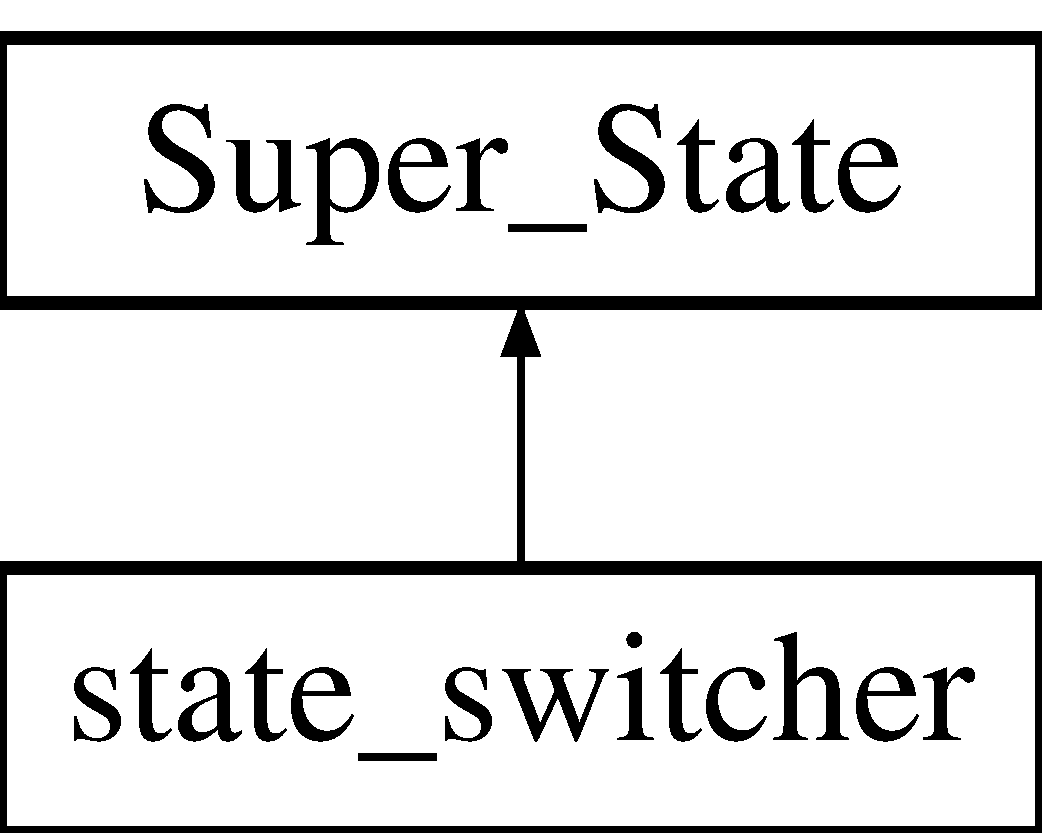
\includegraphics[height=2.000000cm]{classstate__switcher}
\end{center}
\end{figure}
\subsection*{Additional Inherited Members}


\subsection{Detailed Description}


Definition at line 10 of file state\+\_\+switcher.\+h.



The documentation for this class was generated from the following files\+:\begin{DoxyCompactItemize}
\item 
States/\hyperlink{state__switcher_8h}{state\+\_\+switcher.\+h}\item 
States/\hyperlink{state__switcher_8cpp}{state\+\_\+switcher.\+cpp}\end{DoxyCompactItemize}

\hypertarget{class_super___class}{}\section{Super\+\_\+\+Class Class Reference}
\label{class_super___class}\index{Super\+\_\+\+Class@{Super\+\_\+\+Class}}


{\ttfamily \#include $<$Super\+\_\+\+Class.\+h$>$}

Inheritance diagram for Super\+\_\+\+Class\+:\begin{figure}[H]
\begin{center}
\leavevmode
\includegraphics[height=12.000000cm]{class_super___class}
\end{center}
\end{figure}
\subsection*{Public Member Functions}
\begin{DoxyCompactItemize}
\item 
float \hyperlink{class_super___class_ad003a78eaa20b2e4b2ab290f2d353829}{getX} ()
\item 
void \hyperlink{class_super___class_a723decaf337e535db49844408911198e}{setX} (float \hyperlink{class_super___class_a6c644a695141db808e5f1227537e3074}{x})
\item 
float \hyperlink{class_super___class_a9d4c62222b9bec910d8e9b600a853329}{getY} ()
\item 
void \hyperlink{class_super___class_a8f67cb1646ea619e9fc69b9c812fec45}{setY} (float \hyperlink{class_super___class_a340cf4d44abcfb96410f02adcb1d9208}{y})
\end{DoxyCompactItemize}
\subsection*{Protected Attributes}
\begin{DoxyCompactItemize}
\item 
float \hyperlink{class_super___class_a6c644a695141db808e5f1227537e3074}{x}
\item 
float \hyperlink{class_super___class_a340cf4d44abcfb96410f02adcb1d9208}{y}
\end{DoxyCompactItemize}


\subsection{Detailed Description}


Definition at line 10 of file Super\+\_\+\+Class.\+h.



\subsection{Member Function Documentation}
\hypertarget{class_super___class_ad003a78eaa20b2e4b2ab290f2d353829}{}\label{class_super___class_ad003a78eaa20b2e4b2ab290f2d353829} 
\index{Super\+\_\+\+Class@{Super\+\_\+\+Class}!getX@{getX}}
\index{getX@{getX}!Super\+\_\+\+Class@{Super\+\_\+\+Class}}
\subsubsection{\texorpdfstring{get\+X()}{getX()}}
{\footnotesize\ttfamily float Super\+\_\+\+Class\+::getX (\begin{DoxyParamCaption}{ }\end{DoxyParamCaption})}



Definition at line 6 of file Super\+\_\+\+Class.\+cpp.

\hypertarget{class_super___class_a9d4c62222b9bec910d8e9b600a853329}{}\label{class_super___class_a9d4c62222b9bec910d8e9b600a853329} 
\index{Super\+\_\+\+Class@{Super\+\_\+\+Class}!getY@{getY}}
\index{getY@{getY}!Super\+\_\+\+Class@{Super\+\_\+\+Class}}
\subsubsection{\texorpdfstring{get\+Y()}{getY()}}
{\footnotesize\ttfamily float Super\+\_\+\+Class\+::getY (\begin{DoxyParamCaption}{ }\end{DoxyParamCaption})}



Definition at line 14 of file Super\+\_\+\+Class.\+cpp.

\hypertarget{class_super___class_a723decaf337e535db49844408911198e}{}\label{class_super___class_a723decaf337e535db49844408911198e} 
\index{Super\+\_\+\+Class@{Super\+\_\+\+Class}!setX@{setX}}
\index{setX@{setX}!Super\+\_\+\+Class@{Super\+\_\+\+Class}}
\subsubsection{\texorpdfstring{set\+X()}{setX()}}
{\footnotesize\ttfamily void Super\+\_\+\+Class\+::setX (\begin{DoxyParamCaption}\item[{float}]{x }\end{DoxyParamCaption})}



Definition at line 10 of file Super\+\_\+\+Class.\+cpp.

\hypertarget{class_super___class_a8f67cb1646ea619e9fc69b9c812fec45}{}\label{class_super___class_a8f67cb1646ea619e9fc69b9c812fec45} 
\index{Super\+\_\+\+Class@{Super\+\_\+\+Class}!setY@{setY}}
\index{setY@{setY}!Super\+\_\+\+Class@{Super\+\_\+\+Class}}
\subsubsection{\texorpdfstring{set\+Y()}{setY()}}
{\footnotesize\ttfamily void Super\+\_\+\+Class\+::setY (\begin{DoxyParamCaption}\item[{float}]{y }\end{DoxyParamCaption})}



Definition at line 18 of file Super\+\_\+\+Class.\+cpp.



\subsection{Member Data Documentation}
\hypertarget{class_super___class_a6c644a695141db808e5f1227537e3074}{}\label{class_super___class_a6c644a695141db808e5f1227537e3074} 
\index{Super\+\_\+\+Class@{Super\+\_\+\+Class}!x@{x}}
\index{x@{x}!Super\+\_\+\+Class@{Super\+\_\+\+Class}}
\subsubsection{\texorpdfstring{x}{x}}
{\footnotesize\ttfamily float Super\+\_\+\+Class\+::x\hspace{0.3cm}{\ttfamily [protected]}}



Definition at line 13 of file Super\+\_\+\+Class.\+h.

\hypertarget{class_super___class_a340cf4d44abcfb96410f02adcb1d9208}{}\label{class_super___class_a340cf4d44abcfb96410f02adcb1d9208} 
\index{Super\+\_\+\+Class@{Super\+\_\+\+Class}!y@{y}}
\index{y@{y}!Super\+\_\+\+Class@{Super\+\_\+\+Class}}
\subsubsection{\texorpdfstring{y}{y}}
{\footnotesize\ttfamily float Super\+\_\+\+Class\+::y\hspace{0.3cm}{\ttfamily [protected]}}



Definition at line 14 of file Super\+\_\+\+Class.\+h.



The documentation for this class was generated from the following files\+:\begin{DoxyCompactItemize}
\item 
\hyperlink{_super___class_8h}{Super\+\_\+\+Class.\+h}\item 
\hyperlink{_super___class_8cpp}{Super\+\_\+\+Class.\+cpp}\end{DoxyCompactItemize}

\hypertarget{class_super___state}{}\section{Super\+\_\+\+State Class Reference}
\label{class_super___state}\index{Super\+\_\+\+State@{Super\+\_\+\+State}}


{\ttfamily \#include $<$Super\+\_\+\+State.\+h$>$}

Inheritance diagram for Super\+\_\+\+State\+:\begin{figure}[H]
\begin{center}
\leavevmode
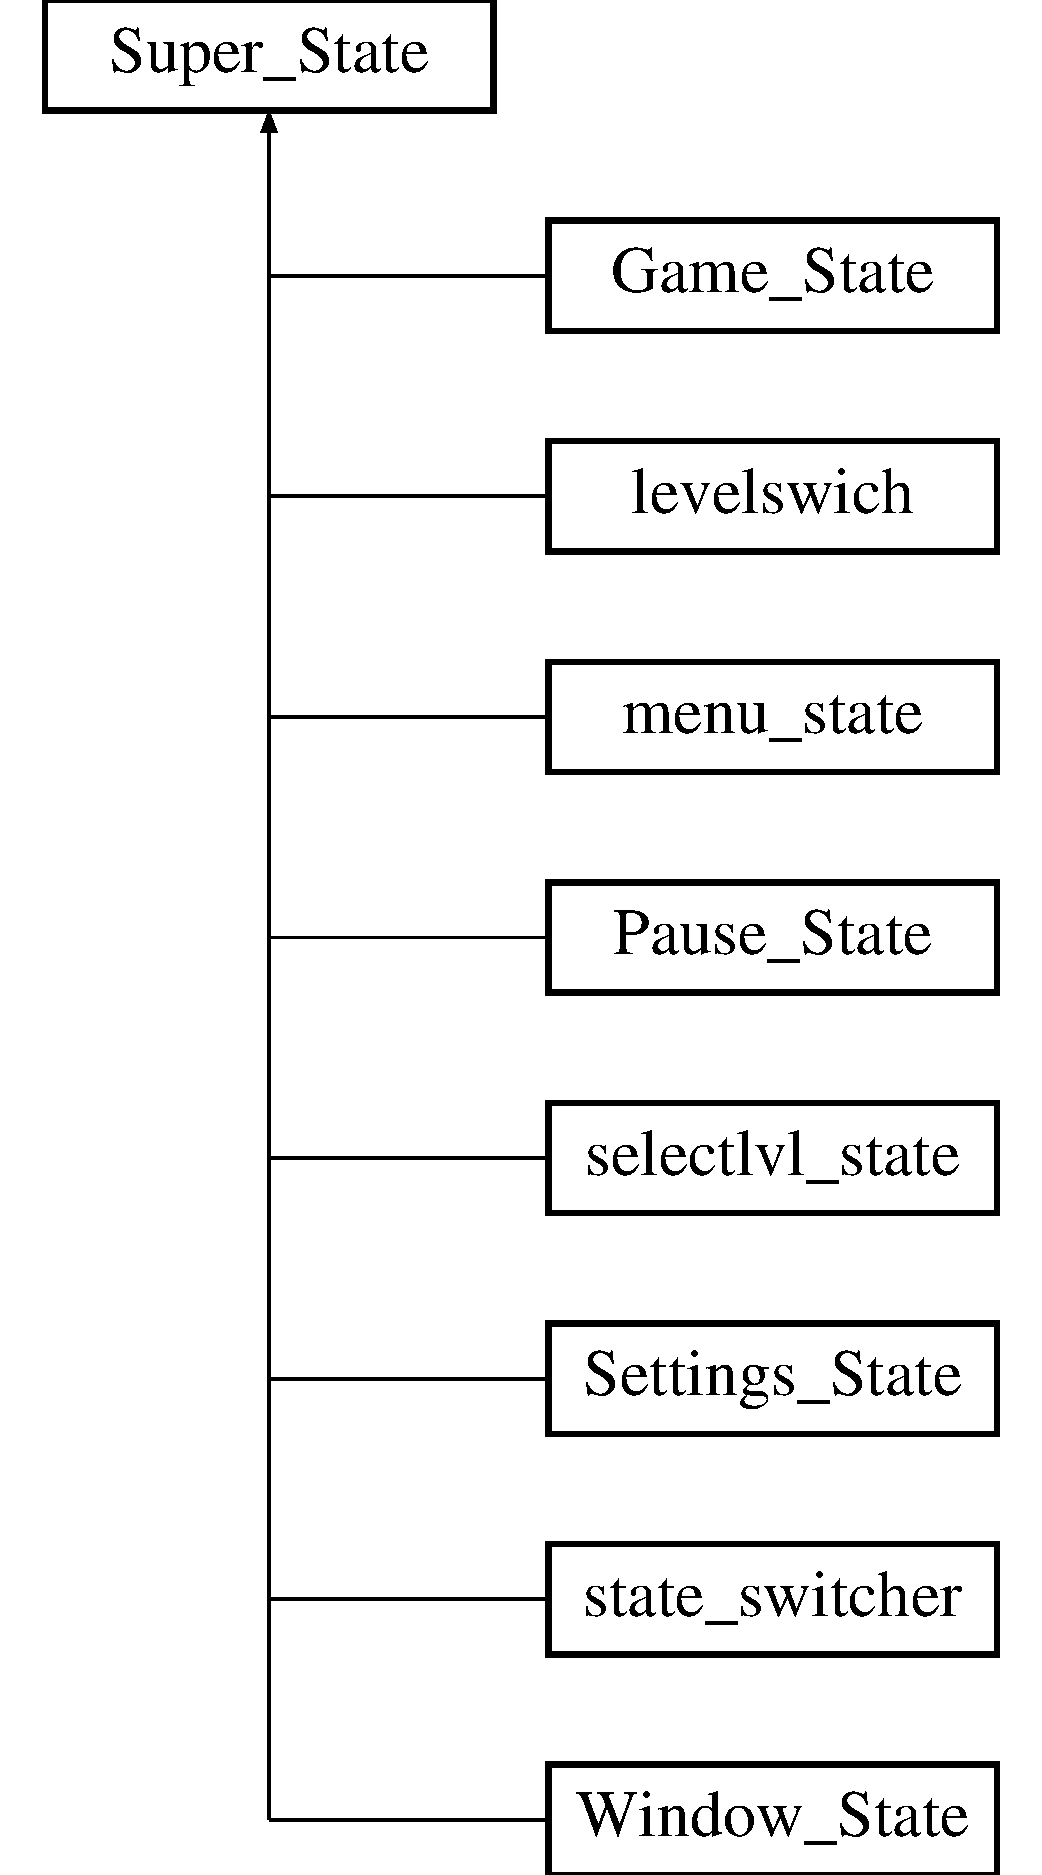
\includegraphics[height=9.000000cm]{class_super___state}
\end{center}
\end{figure}
\subsection*{Public Member Functions}
\begin{DoxyCompactItemize}
\item 
void \hyperlink{class_super___state_a2f0cf545a5099f59e1c0bf87423ee846}{switch\+To} ()
\end{DoxyCompactItemize}
\subsection*{Public Attributes}
\begin{DoxyCompactItemize}
\item 
int \hyperlink{class_super___state_a5f3b37d247498fd969869834ab7904fa}{stateid} =0
\item 
int \hyperlink{class_super___state_ad6b74d4864a4e2cccf58316cd1af2e83}{level} = -\/1
\end{DoxyCompactItemize}


\subsection{Detailed Description}


Definition at line 12 of file Super\+\_\+\+State.\+h.



\subsection{Member Function Documentation}
\hypertarget{class_super___state_a2f0cf545a5099f59e1c0bf87423ee846}{}\label{class_super___state_a2f0cf545a5099f59e1c0bf87423ee846} 
\index{Super\+\_\+\+State@{Super\+\_\+\+State}!switch\+To@{switch\+To}}
\index{switch\+To@{switch\+To}!Super\+\_\+\+State@{Super\+\_\+\+State}}
\subsubsection{\texorpdfstring{switch\+To()}{switchTo()}}
{\footnotesize\ttfamily void Super\+\_\+\+State\+::switch\+To (\begin{DoxyParamCaption}{ }\end{DoxyParamCaption})}



\subsection{Member Data Documentation}
\hypertarget{class_super___state_ad6b74d4864a4e2cccf58316cd1af2e83}{}\label{class_super___state_ad6b74d4864a4e2cccf58316cd1af2e83} 
\index{Super\+\_\+\+State@{Super\+\_\+\+State}!level@{level}}
\index{level@{level}!Super\+\_\+\+State@{Super\+\_\+\+State}}
\subsubsection{\texorpdfstring{level}{level}}
{\footnotesize\ttfamily int Super\+\_\+\+State\+::level = -\/1}



Definition at line 15 of file Super\+\_\+\+State.\+h.

\hypertarget{class_super___state_a5f3b37d247498fd969869834ab7904fa}{}\label{class_super___state_a5f3b37d247498fd969869834ab7904fa} 
\index{Super\+\_\+\+State@{Super\+\_\+\+State}!stateid@{stateid}}
\index{stateid@{stateid}!Super\+\_\+\+State@{Super\+\_\+\+State}}
\subsubsection{\texorpdfstring{stateid}{stateid}}
{\footnotesize\ttfamily int Super\+\_\+\+State\+::stateid =0}



Definition at line 14 of file Super\+\_\+\+State.\+h.



The documentation for this class was generated from the following file\+:\begin{DoxyCompactItemize}
\item 
States/\hyperlink{_super___state_8h}{Super\+\_\+\+State.\+h}\end{DoxyCompactItemize}

\hypertarget{class_super___tile}{}\section{Super\+\_\+\+Tile Class Reference}
\label{class_super___tile}\index{Super\+\_\+\+Tile@{Super\+\_\+\+Tile}}


{\ttfamily \#include $<$Super\+\_\+\+Tile.\+h$>$}

Inheritance diagram for Super\+\_\+\+Tile\+:\begin{figure}[H]
\begin{center}
\leavevmode
\includegraphics[height=2.800000cm]{class_super___tile}
\end{center}
\end{figure}
\subsection*{Public Member Functions}
\begin{DoxyCompactItemize}
\item 
virtual void \hyperlink{class_super___tile_a7b509383d0d0ad2df0220f7dc4660823}{impact} (\hyperlink{class_actor___class}{Actor\+\_\+\+Class} $\ast$actor)
\end{DoxyCompactItemize}
\subsection*{Public Attributes}
\begin{DoxyCompactItemize}
\item 
int \hyperlink{class_super___tile_afc4dffc7fdb4919c9790e1634c909698}{id} = 0
\item 
sf\+::\+Vector2f \hyperlink{class_super___tile_ad6bcea1fd54f67808f54ba2aacd88596}{nw}
\item 
sf\+::\+Vector2f \hyperlink{class_super___tile_a55f6d2860da36f13019bd4e0d18364ca}{ne}
\item 
sf\+::\+Vector2f \hyperlink{class_super___tile_abe9efe0c3d1ed440395225843435dfc8}{sw}
\item 
sf\+::\+Vector2f \hyperlink{class_super___tile_ab384b89a7a631b8b75c4d405c51a23e1}{se}
\item 
bool \hyperlink{class_super___tile_af486363a0321c167562c54da0f04884c}{solid} = true
\item 
int \hyperlink{class_super___tile_a11736ca52512c43b001d69a805c83de5}{direction}
\end{DoxyCompactItemize}


\subsection{Detailed Description}


Definition at line 12 of file Super\+\_\+\+Tile.\+h.



\subsection{Member Function Documentation}
\hypertarget{class_super___tile_a7b509383d0d0ad2df0220f7dc4660823}{}\label{class_super___tile_a7b509383d0d0ad2df0220f7dc4660823} 
\index{Super\+\_\+\+Tile@{Super\+\_\+\+Tile}!impact@{impact}}
\index{impact@{impact}!Super\+\_\+\+Tile@{Super\+\_\+\+Tile}}
\subsubsection{\texorpdfstring{impact()}{impact()}}
{\footnotesize\ttfamily void Super\+\_\+\+Tile\+::impact (\begin{DoxyParamCaption}\item[{\hyperlink{class_actor___class}{Actor\+\_\+\+Class} $\ast$}]{actor }\end{DoxyParamCaption})\hspace{0.3cm}{\ttfamily [virtual]}}



Reimplemented in \hyperlink{class_finnish__tile_a04fae2c808c18027ec8b74915df33220}{Finnish\+\_\+tile}, \hyperlink{class_spawn___tile_a9b557377a8afd06512ac19368a4f14a4}{Spawn\+\_\+\+Tile}, \hyperlink{class_spike___tile_a8673c82f84733fe73c456eee725a6ab0}{Spike\+\_\+\+Tile}, \hyperlink{class_solid___tile_ada34ec00762b7df804292f40fbeecc95}{Solid\+\_\+\+Tile}, \hyperlink{class_action___tile_aa366fba2ea9d3947c28c45f939ee0217}{Action\+\_\+\+Tile}, \hyperlink{class_semisolid___tile_a65c8e43f414282be042b81c62fc63431}{Semisolid\+\_\+\+Tile}, and \hyperlink{class_speed___tile_aea424ba028f29398ace251a3a664b874}{Speed\+\_\+\+Tile}.



Definition at line 4 of file Super\+\_\+\+Tile.\+cpp.



\subsection{Member Data Documentation}
\hypertarget{class_super___tile_a11736ca52512c43b001d69a805c83de5}{}\label{class_super___tile_a11736ca52512c43b001d69a805c83de5} 
\index{Super\+\_\+\+Tile@{Super\+\_\+\+Tile}!direction@{direction}}
\index{direction@{direction}!Super\+\_\+\+Tile@{Super\+\_\+\+Tile}}
\subsubsection{\texorpdfstring{direction}{direction}}
{\footnotesize\ttfamily int Super\+\_\+\+Tile\+::direction}



Definition at line 21 of file Super\+\_\+\+Tile.\+h.

\hypertarget{class_super___tile_afc4dffc7fdb4919c9790e1634c909698}{}\label{class_super___tile_afc4dffc7fdb4919c9790e1634c909698} 
\index{Super\+\_\+\+Tile@{Super\+\_\+\+Tile}!id@{id}}
\index{id@{id}!Super\+\_\+\+Tile@{Super\+\_\+\+Tile}}
\subsubsection{\texorpdfstring{id}{id}}
{\footnotesize\ttfamily int Super\+\_\+\+Tile\+::id = 0}



Definition at line 14 of file Super\+\_\+\+Tile.\+h.

\hypertarget{class_super___tile_a55f6d2860da36f13019bd4e0d18364ca}{}\label{class_super___tile_a55f6d2860da36f13019bd4e0d18364ca} 
\index{Super\+\_\+\+Tile@{Super\+\_\+\+Tile}!ne@{ne}}
\index{ne@{ne}!Super\+\_\+\+Tile@{Super\+\_\+\+Tile}}
\subsubsection{\texorpdfstring{ne}{ne}}
{\footnotesize\ttfamily sf\+::\+Vector2f Super\+\_\+\+Tile\+::ne}



Definition at line 16 of file Super\+\_\+\+Tile.\+h.

\hypertarget{class_super___tile_ad6bcea1fd54f67808f54ba2aacd88596}{}\label{class_super___tile_ad6bcea1fd54f67808f54ba2aacd88596} 
\index{Super\+\_\+\+Tile@{Super\+\_\+\+Tile}!nw@{nw}}
\index{nw@{nw}!Super\+\_\+\+Tile@{Super\+\_\+\+Tile}}
\subsubsection{\texorpdfstring{nw}{nw}}
{\footnotesize\ttfamily sf\+::\+Vector2f Super\+\_\+\+Tile\+::nw}



Definition at line 15 of file Super\+\_\+\+Tile.\+h.

\hypertarget{class_super___tile_ab384b89a7a631b8b75c4d405c51a23e1}{}\label{class_super___tile_ab384b89a7a631b8b75c4d405c51a23e1} 
\index{Super\+\_\+\+Tile@{Super\+\_\+\+Tile}!se@{se}}
\index{se@{se}!Super\+\_\+\+Tile@{Super\+\_\+\+Tile}}
\subsubsection{\texorpdfstring{se}{se}}
{\footnotesize\ttfamily sf\+::\+Vector2f Super\+\_\+\+Tile\+::se}



Definition at line 18 of file Super\+\_\+\+Tile.\+h.

\hypertarget{class_super___tile_af486363a0321c167562c54da0f04884c}{}\label{class_super___tile_af486363a0321c167562c54da0f04884c} 
\index{Super\+\_\+\+Tile@{Super\+\_\+\+Tile}!solid@{solid}}
\index{solid@{solid}!Super\+\_\+\+Tile@{Super\+\_\+\+Tile}}
\subsubsection{\texorpdfstring{solid}{solid}}
{\footnotesize\ttfamily bool Super\+\_\+\+Tile\+::solid = true}



Definition at line 20 of file Super\+\_\+\+Tile.\+h.

\hypertarget{class_super___tile_abe9efe0c3d1ed440395225843435dfc8}{}\label{class_super___tile_abe9efe0c3d1ed440395225843435dfc8} 
\index{Super\+\_\+\+Tile@{Super\+\_\+\+Tile}!sw@{sw}}
\index{sw@{sw}!Super\+\_\+\+Tile@{Super\+\_\+\+Tile}}
\subsubsection{\texorpdfstring{sw}{sw}}
{\footnotesize\ttfamily sf\+::\+Vector2f Super\+\_\+\+Tile\+::sw}



Definition at line 17 of file Super\+\_\+\+Tile.\+h.



The documentation for this class was generated from the following files\+:\begin{DoxyCompactItemize}
\item 
Tile/\hyperlink{_super___tile_8h}{Super\+\_\+\+Tile.\+h}\item 
Tile/\hyperlink{_super___tile_8cpp}{Super\+\_\+\+Tile.\+cpp}\end{DoxyCompactItemize}

\hypertarget{class_textbox}{}\section{Textbox Class Reference}
\label{class_textbox}\index{Textbox@{Textbox}}


{\ttfamily \#include $<$Textbox.\+h$>$}

Inheritance diagram for Textbox\+:\begin{figure}[H]
\begin{center}
\leavevmode
\includegraphics[height=3.000000cm]{class_textbox}
\end{center}
\end{figure}
\subsection*{Public Member Functions}
\begin{DoxyCompactItemize}
\item 
\hyperlink{class_textbox_ada0c266e63758f57f6f9c88daed041bd}{Textbox} (sf\+::\+Render\+Window \&window, \hyperlink{class_collision}{Collision} \hyperlink{class_textbox_ad89bdee3ead7d89dca3e1ba1468c272c}{col}, int x\+Inn, int y\+Inn)
\item 
void \hyperlink{class_textbox_a0a58c0b828fb627bd21c8156d279e082}{load\+Text} (int select)
\item 
void \hyperlink{class_textbox_a995336eb1a269216afb4dcd187e39d0b}{jump} ()
\item 
void \hyperlink{class_textbox_a4680a3e6bbaa33dc57a585c7e0072b0a}{move} ()
\item 
void \hyperlink{class_textbox_a164e6dfbd1964b36b05de0cf84d07abf}{draw} ()
\item 
void \hyperlink{class_textbox_a830cca6316662b4c7a1ae1d2f844f9ae}{death} ()
\item 
void \hyperlink{class_textbox_a67dd5640da6bbd88affded4a37ede098}{interaction} (std\+::vector$<$ \hyperlink{class_actor___class}{Actor\+\_\+\+Class} $\ast$$>$ actor\+\_\+array)
\end{DoxyCompactItemize}
\subsection*{Public Attributes}
\begin{DoxyCompactItemize}
\item 
sf\+::\+Text \hyperlink{class_textbox_a4f79784c45871da706e57c8435c8dff3}{text}
\item 
sf\+::\+Text \hyperlink{class_textbox_a5c229bd6795f3ab970ee0bf10252613d}{text1}
\item 
sf\+::\+Text \hyperlink{class_textbox_adafebfa39688753f259c72a7fcdcc3ad}{text2}
\item 
sf\+::\+Text \hyperlink{class_textbox_abccc498be23e0a6d7271a4692ae50289}{text3}
\item 
sf\+::\+Text \hyperlink{class_textbox_a37cfcc698bdbb5014fdc6ecf56c083c8}{text4}
\item 
sf\+::\+Text \hyperlink{class_textbox_a4f9b578979f37d545571532e41148a45}{text5}
\item 
sf\+::\+Font \hyperlink{class_textbox_a45eac53d4f51e36a8c0acfdc9df2f0cb}{font}
\item 
sf\+::\+Rectangle\+Shape \hyperlink{class_textbox_a6da196e36384e83b7dc9fa9f81848536}{textbox}
\item 
sf\+::\+Render\+Window \& \hyperlink{class_textbox_a43cc0d802e43397e373997b8595073ad}{vindu}
\item 
\hyperlink{class_collision}{Collision} \hyperlink{class_textbox_ad89bdee3ead7d89dca3e1ba1468c272c}{col}
\item 
int \hyperlink{class_textbox_a8b9942b46c9fab7ed505918750174006}{startX} =400
\begin{DoxyCompactList}\small\item\em float floor =400;//bør byttes ut med at det er localisasjonen den intersecter med en title \end{DoxyCompactList}\item 
int \hyperlink{class_textbox_a7cc50c3fa4ef2866a7d2acc7f2d5565b}{startY} =20
\end{DoxyCompactItemize}
\subsection*{Additional Inherited Members}


\subsection{Detailed Description}


Definition at line 15 of file Textbox.\+h.



\subsection{Constructor \& Destructor Documentation}
\hypertarget{class_textbox_ada0c266e63758f57f6f9c88daed041bd}{}\label{class_textbox_ada0c266e63758f57f6f9c88daed041bd} 
\index{Textbox@{Textbox}!Textbox@{Textbox}}
\index{Textbox@{Textbox}!Textbox@{Textbox}}
\subsubsection{\texorpdfstring{Textbox()}{Textbox()}}
{\footnotesize\ttfamily Textbox\+::\+Textbox (\begin{DoxyParamCaption}\item[{sf\+::\+Render\+Window \&}]{window,  }\item[{\hyperlink{class_collision}{Collision}}]{col,  }\item[{int}]{x\+Inn,  }\item[{int}]{y\+Inn }\end{DoxyParamCaption})}



Definition at line 7 of file Textbox.\+cpp.



\subsection{Member Function Documentation}
\hypertarget{class_textbox_a830cca6316662b4c7a1ae1d2f844f9ae}{}\label{class_textbox_a830cca6316662b4c7a1ae1d2f844f9ae} 
\index{Textbox@{Textbox}!death@{death}}
\index{death@{death}!Textbox@{Textbox}}
\subsubsection{\texorpdfstring{death()}{death()}}
{\footnotesize\ttfamily void Textbox\+::death (\begin{DoxyParamCaption}{ }\end{DoxyParamCaption})\hspace{0.3cm}{\ttfamily [virtual]}}



Reimplemented from \hyperlink{class_actor___class_a9447c6154a674d7e6bdf24ff2874b7a8}{Actor\+\_\+\+Class}.



Definition at line 154 of file Textbox.\+cpp.

\hypertarget{class_textbox_a164e6dfbd1964b36b05de0cf84d07abf}{}\label{class_textbox_a164e6dfbd1964b36b05de0cf84d07abf} 
\index{Textbox@{Textbox}!draw@{draw}}
\index{draw@{draw}!Textbox@{Textbox}}
\subsubsection{\texorpdfstring{draw()}{draw()}}
{\footnotesize\ttfamily void Textbox\+::draw (\begin{DoxyParamCaption}{ }\end{DoxyParamCaption})\hspace{0.3cm}{\ttfamily [virtual]}}



Reimplemented from \hyperlink{class_actor___class_ac49cd62be76b4b950ecbe155413f1b64}{Actor\+\_\+\+Class}.



Definition at line 110 of file Textbox.\+cpp.

\hypertarget{class_textbox_a67dd5640da6bbd88affded4a37ede098}{}\label{class_textbox_a67dd5640da6bbd88affded4a37ede098} 
\index{Textbox@{Textbox}!interaction@{interaction}}
\index{interaction@{interaction}!Textbox@{Textbox}}
\subsubsection{\texorpdfstring{interaction()}{interaction()}}
{\footnotesize\ttfamily void Textbox\+::interaction (\begin{DoxyParamCaption}\item[{std\+::vector$<$ \hyperlink{class_actor___class}{Actor\+\_\+\+Class} $\ast$$>$}]{actor\+\_\+array }\end{DoxyParamCaption})\hspace{0.3cm}{\ttfamily [virtual]}}



Reimplemented from \hyperlink{class_actor___class_a87d1e079d8576fa99592a60b38a04a1b}{Actor\+\_\+\+Class}.



Definition at line 122 of file Textbox.\+cpp.

\hypertarget{class_textbox_a995336eb1a269216afb4dcd187e39d0b}{}\label{class_textbox_a995336eb1a269216afb4dcd187e39d0b} 
\index{Textbox@{Textbox}!jump@{jump}}
\index{jump@{jump}!Textbox@{Textbox}}
\subsubsection{\texorpdfstring{jump()}{jump()}}
{\footnotesize\ttfamily void Textbox\+::jump (\begin{DoxyParamCaption}{ }\end{DoxyParamCaption})\hspace{0.3cm}{\ttfamily [virtual]}}



Reimplemented from \hyperlink{class_actor___class_ab33216a3ce0c856bdc16231c71ae35c2}{Actor\+\_\+\+Class}.



Definition at line 151 of file Textbox.\+cpp.

\hypertarget{class_textbox_a0a58c0b828fb627bd21c8156d279e082}{}\label{class_textbox_a0a58c0b828fb627bd21c8156d279e082} 
\index{Textbox@{Textbox}!load\+Text@{load\+Text}}
\index{load\+Text@{load\+Text}!Textbox@{Textbox}}
\subsubsection{\texorpdfstring{load\+Text()}{loadText()}}
{\footnotesize\ttfamily void Textbox\+::load\+Text (\begin{DoxyParamCaption}\item[{int}]{select }\end{DoxyParamCaption})}



Definition at line 71 of file Textbox.\+cpp.

\hypertarget{class_textbox_a4680a3e6bbaa33dc57a585c7e0072b0a}{}\label{class_textbox_a4680a3e6bbaa33dc57a585c7e0072b0a} 
\index{Textbox@{Textbox}!move@{move}}
\index{move@{move}!Textbox@{Textbox}}
\subsubsection{\texorpdfstring{move()}{move()}}
{\footnotesize\ttfamily void Textbox\+::move (\begin{DoxyParamCaption}{ }\end{DoxyParamCaption})\hspace{0.3cm}{\ttfamily [virtual]}}



Reimplemented from \hyperlink{class_actor___class_af1764a94c5410ba8476f56553cd2c327}{Actor\+\_\+\+Class}.



Definition at line 66 of file Textbox.\+cpp.



\subsection{Member Data Documentation}
\hypertarget{class_textbox_ad89bdee3ead7d89dca3e1ba1468c272c}{}\label{class_textbox_ad89bdee3ead7d89dca3e1ba1468c272c} 
\index{Textbox@{Textbox}!col@{col}}
\index{col@{col}!Textbox@{Textbox}}
\subsubsection{\texorpdfstring{col}{col}}
{\footnotesize\ttfamily \hyperlink{class_collision}{Collision} Textbox\+::col}



Definition at line 33 of file Textbox.\+h.

\hypertarget{class_textbox_a45eac53d4f51e36a8c0acfdc9df2f0cb}{}\label{class_textbox_a45eac53d4f51e36a8c0acfdc9df2f0cb} 
\index{Textbox@{Textbox}!font@{font}}
\index{font@{font}!Textbox@{Textbox}}
\subsubsection{\texorpdfstring{font}{font}}
{\footnotesize\ttfamily sf\+::\+Font Textbox\+::font}



Definition at line 27 of file Textbox.\+h.

\hypertarget{class_textbox_a8b9942b46c9fab7ed505918750174006}{}\label{class_textbox_a8b9942b46c9fab7ed505918750174006} 
\index{Textbox@{Textbox}!startX@{startX}}
\index{startX@{startX}!Textbox@{Textbox}}
\subsubsection{\texorpdfstring{startX}{startX}}
{\footnotesize\ttfamily int Textbox\+::startX =400}



float floor =400;//bør byttes ut med at det er localisasjonen den intersecter med en title 



Definition at line 41 of file Textbox.\+h.

\hypertarget{class_textbox_a7cc50c3fa4ef2866a7d2acc7f2d5565b}{}\label{class_textbox_a7cc50c3fa4ef2866a7d2acc7f2d5565b} 
\index{Textbox@{Textbox}!startY@{startY}}
\index{startY@{startY}!Textbox@{Textbox}}
\subsubsection{\texorpdfstring{startY}{startY}}
{\footnotesize\ttfamily int Textbox\+::startY =20}



Definition at line 42 of file Textbox.\+h.

\hypertarget{class_textbox_a4f79784c45871da706e57c8435c8dff3}{}\label{class_textbox_a4f79784c45871da706e57c8435c8dff3} 
\index{Textbox@{Textbox}!text@{text}}
\index{text@{text}!Textbox@{Textbox}}
\subsubsection{\texorpdfstring{text}{text}}
{\footnotesize\ttfamily sf\+::\+Text Textbox\+::text}



Definition at line 21 of file Textbox.\+h.

\hypertarget{class_textbox_a5c229bd6795f3ab970ee0bf10252613d}{}\label{class_textbox_a5c229bd6795f3ab970ee0bf10252613d} 
\index{Textbox@{Textbox}!text1@{text1}}
\index{text1@{text1}!Textbox@{Textbox}}
\subsubsection{\texorpdfstring{text1}{text1}}
{\footnotesize\ttfamily sf\+::\+Text Textbox\+::text1}



Definition at line 22 of file Textbox.\+h.

\hypertarget{class_textbox_adafebfa39688753f259c72a7fcdcc3ad}{}\label{class_textbox_adafebfa39688753f259c72a7fcdcc3ad} 
\index{Textbox@{Textbox}!text2@{text2}}
\index{text2@{text2}!Textbox@{Textbox}}
\subsubsection{\texorpdfstring{text2}{text2}}
{\footnotesize\ttfamily sf\+::\+Text Textbox\+::text2}



Definition at line 23 of file Textbox.\+h.

\hypertarget{class_textbox_abccc498be23e0a6d7271a4692ae50289}{}\label{class_textbox_abccc498be23e0a6d7271a4692ae50289} 
\index{Textbox@{Textbox}!text3@{text3}}
\index{text3@{text3}!Textbox@{Textbox}}
\subsubsection{\texorpdfstring{text3}{text3}}
{\footnotesize\ttfamily sf\+::\+Text Textbox\+::text3}



Definition at line 24 of file Textbox.\+h.

\hypertarget{class_textbox_a37cfcc698bdbb5014fdc6ecf56c083c8}{}\label{class_textbox_a37cfcc698bdbb5014fdc6ecf56c083c8} 
\index{Textbox@{Textbox}!text4@{text4}}
\index{text4@{text4}!Textbox@{Textbox}}
\subsubsection{\texorpdfstring{text4}{text4}}
{\footnotesize\ttfamily sf\+::\+Text Textbox\+::text4}



Definition at line 25 of file Textbox.\+h.

\hypertarget{class_textbox_a4f9b578979f37d545571532e41148a45}{}\label{class_textbox_a4f9b578979f37d545571532e41148a45} 
\index{Textbox@{Textbox}!text5@{text5}}
\index{text5@{text5}!Textbox@{Textbox}}
\subsubsection{\texorpdfstring{text5}{text5}}
{\footnotesize\ttfamily sf\+::\+Text Textbox\+::text5}



Definition at line 26 of file Textbox.\+h.

\hypertarget{class_textbox_a6da196e36384e83b7dc9fa9f81848536}{}\label{class_textbox_a6da196e36384e83b7dc9fa9f81848536} 
\index{Textbox@{Textbox}!textbox@{textbox}}
\index{textbox@{textbox}!Textbox@{Textbox}}
\subsubsection{\texorpdfstring{textbox}{textbox}}
{\footnotesize\ttfamily sf\+::\+Rectangle\+Shape Textbox\+::textbox}



Definition at line 30 of file Textbox.\+h.

\hypertarget{class_textbox_a43cc0d802e43397e373997b8595073ad}{}\label{class_textbox_a43cc0d802e43397e373997b8595073ad} 
\index{Textbox@{Textbox}!vindu@{vindu}}
\index{vindu@{vindu}!Textbox@{Textbox}}
\subsubsection{\texorpdfstring{vindu}{vindu}}
{\footnotesize\ttfamily sf\+::\+Render\+Window\& Textbox\+::vindu}



Definition at line 32 of file Textbox.\+h.



The documentation for this class was generated from the following files\+:\begin{DoxyCompactItemize}
\item 
Actor/\hyperlink{_textbox_8h}{Textbox.\+h}\item 
Actor/\hyperlink{_textbox_8cpp}{Textbox.\+cpp}\end{DoxyCompactItemize}

\hypertarget{class_tilemap}{}\section{Tilemap Class Reference}
\label{class_tilemap}\index{Tilemap@{Tilemap}}


{\ttfamily \#include $<$Tilemap.\+h$>$}

Inheritance diagram for Tilemap\+:\begin{figure}[H]
\begin{center}
\leavevmode
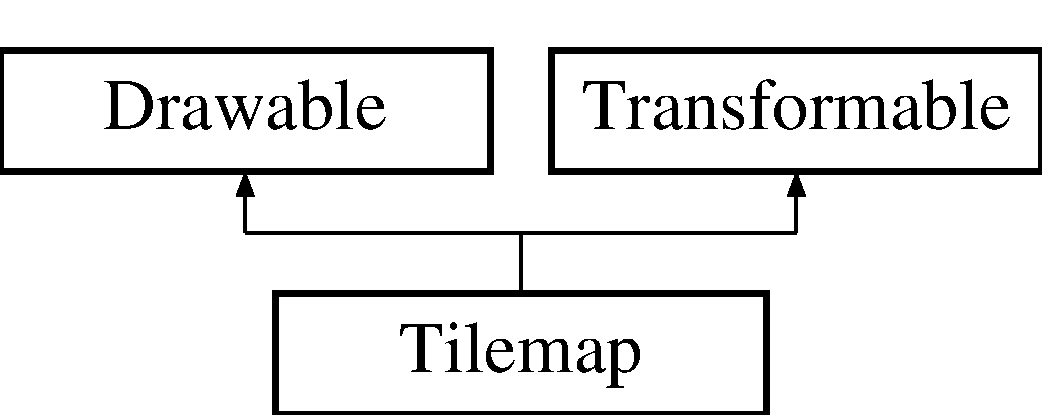
\includegraphics[height=2.000000cm]{class_tilemap}
\end{center}
\end{figure}
\subsection*{Public Member Functions}
\begin{DoxyCompactItemize}
\item 
std\+::vector$<$ int $>$ \hyperlink{class_tilemap_aaf6018db69a5590cd7346bd4de98fc35}{load\+Map\+From\+File} (std\+::string level\+Loc)
\item 
bool \hyperlink{class_tilemap_a20ae966645360ac69d313811539dcbcc}{load} (\hyperlink{class_level}{Level} lastet\+Level)
\item 
void \hyperlink{class_tilemap_aa987cd1aa8ebf71dbe2333dafe2b4039}{sort\+Spawn\+List} ()
\end{DoxyCompactItemize}
\subsection*{Public Attributes}
\begin{DoxyCompactItemize}
\item 
std\+::vector$<$ \hyperlink{class_super___tile}{Super\+\_\+\+Tile} $\ast$ $>$ \hyperlink{class_tilemap_a49439fd862d03bdcc26d0c3b5156bc7a}{tile\+List}
\item 
std\+::vector$<$ \hyperlink{class_solid___tile}{Solid\+\_\+\+Tile} $\ast$ $>$ \hyperlink{class_tilemap_aecd9cc5f70702439e13fd6213d176f14}{solid\+Tile\+List}
\item 
std\+::vector$<$ \hyperlink{class_action___tile}{Action\+\_\+\+Tile} $\ast$ $>$ \hyperlink{class_tilemap_ad855bfd20bf768d4f712fe40c5fcaeea}{action\+Tile\+List}
\item 
std\+::vector$<$ \hyperlink{class_spawn___tile}{Spawn\+\_\+\+Tile} $\ast$ $>$ \hyperlink{class_tilemap_a41ae114e32893255ef339dd26c635039}{spawn\+Tile\+List}
\item 
\hyperlink{class_spawn___tile}{Spawn\+\_\+\+Tile} $\ast$ \hyperlink{class_tilemap_a0b9b8cb0dae83e1729ac5d1cc8411395}{hero\+Spawn}
\item 
int \hyperlink{class_tilemap_a20a5ecfd38a3612d4294eb19da4f36ea}{length}
\item 
int \hyperlink{class_tilemap_a65d3108ef1805edef0df66843e8d5e6a}{height}
\item 
int \hyperlink{class_tilemap_a07d9546ed98a4da502902ebaa1d774ca}{tilesize}
\item 
bool \hyperlink{class_tilemap_af966f7c50449d758cb11abdec5767f64}{destroyed} = false
\end{DoxyCompactItemize}


\subsection{Detailed Description}


Definition at line 24 of file Tilemap.\+h.



\subsection{Member Function Documentation}
\hypertarget{class_tilemap_a20ae966645360ac69d313811539dcbcc}{}\label{class_tilemap_a20ae966645360ac69d313811539dcbcc} 
\index{Tilemap@{Tilemap}!load@{load}}
\index{load@{load}!Tilemap@{Tilemap}}
\subsubsection{\texorpdfstring{load()}{load()}}
{\footnotesize\ttfamily bool Tilemap\+::load (\begin{DoxyParamCaption}\item[{\hyperlink{class_level}{Level}}]{lastet\+Level }\end{DoxyParamCaption})}

Laster inn teksturer og mapper dem til skjermen. Lagrer solide tiles inn i et array kalt tile\+List 
\begin{DoxyParams}{Parameters}
{\em level\+Loc} & \\
\hline
\end{DoxyParams}
\begin{DoxyReturn}{Returns}

\end{DoxyReturn}


Definition at line 27 of file Tilemap.\+cpp.

\hypertarget{class_tilemap_aaf6018db69a5590cd7346bd4de98fc35}{}\label{class_tilemap_aaf6018db69a5590cd7346bd4de98fc35} 
\index{Tilemap@{Tilemap}!load\+Map\+From\+File@{load\+Map\+From\+File}}
\index{load\+Map\+From\+File@{load\+Map\+From\+File}!Tilemap@{Tilemap}}
\subsubsection{\texorpdfstring{load\+Map\+From\+File()}{loadMapFromFile()}}
{\footnotesize\ttfamily std\+::vector$<$ int $>$ Tilemap\+::load\+Map\+From\+File (\begin{DoxyParamCaption}\item[{std\+::string}]{level\+Loc }\end{DoxyParamCaption})}

Laster inn txt filen og plasserer tallene in en array. 
\begin{DoxyParams}{Parameters}
{\em level\+Loc} & stedet hvor levelen er lagret \\
\hline
\end{DoxyParams}
\begin{DoxyReturn}{Returns}

\end{DoxyReturn}


Definition at line 8 of file Tilemap.\+cpp.

\hypertarget{class_tilemap_aa987cd1aa8ebf71dbe2333dafe2b4039}{}\label{class_tilemap_aa987cd1aa8ebf71dbe2333dafe2b4039} 
\index{Tilemap@{Tilemap}!sort\+Spawn\+List@{sort\+Spawn\+List}}
\index{sort\+Spawn\+List@{sort\+Spawn\+List}!Tilemap@{Tilemap}}
\subsubsection{\texorpdfstring{sort\+Spawn\+List()}{sortSpawnList()}}
{\footnotesize\ttfamily void Tilemap\+::sort\+Spawn\+List (\begin{DoxyParamCaption}{ }\end{DoxyParamCaption})}



\subsection{Member Data Documentation}
\hypertarget{class_tilemap_ad855bfd20bf768d4f712fe40c5fcaeea}{}\label{class_tilemap_ad855bfd20bf768d4f712fe40c5fcaeea} 
\index{Tilemap@{Tilemap}!action\+Tile\+List@{action\+Tile\+List}}
\index{action\+Tile\+List@{action\+Tile\+List}!Tilemap@{Tilemap}}
\subsubsection{\texorpdfstring{action\+Tile\+List}{actionTileList}}
{\footnotesize\ttfamily std\+::vector$<$\hyperlink{class_action___tile}{Action\+\_\+\+Tile}$\ast$$>$ Tilemap\+::action\+Tile\+List}



Definition at line 28 of file Tilemap.\+h.

\hypertarget{class_tilemap_af966f7c50449d758cb11abdec5767f64}{}\label{class_tilemap_af966f7c50449d758cb11abdec5767f64} 
\index{Tilemap@{Tilemap}!destroyed@{destroyed}}
\index{destroyed@{destroyed}!Tilemap@{Tilemap}}
\subsubsection{\texorpdfstring{destroyed}{destroyed}}
{\footnotesize\ttfamily bool Tilemap\+::destroyed = false}



Definition at line 45 of file Tilemap.\+h.

\hypertarget{class_tilemap_a65d3108ef1805edef0df66843e8d5e6a}{}\label{class_tilemap_a65d3108ef1805edef0df66843e8d5e6a} 
\index{Tilemap@{Tilemap}!height@{height}}
\index{height@{height}!Tilemap@{Tilemap}}
\subsubsection{\texorpdfstring{height}{height}}
{\footnotesize\ttfamily int Tilemap\+::height}



Definition at line 42 of file Tilemap.\+h.

\hypertarget{class_tilemap_a0b9b8cb0dae83e1729ac5d1cc8411395}{}\label{class_tilemap_a0b9b8cb0dae83e1729ac5d1cc8411395} 
\index{Tilemap@{Tilemap}!hero\+Spawn@{hero\+Spawn}}
\index{hero\+Spawn@{hero\+Spawn}!Tilemap@{Tilemap}}
\subsubsection{\texorpdfstring{hero\+Spawn}{heroSpawn}}
{\footnotesize\ttfamily \hyperlink{class_spawn___tile}{Spawn\+\_\+\+Tile}$\ast$ Tilemap\+::hero\+Spawn}



Definition at line 30 of file Tilemap.\+h.

\hypertarget{class_tilemap_a20a5ecfd38a3612d4294eb19da4f36ea}{}\label{class_tilemap_a20a5ecfd38a3612d4294eb19da4f36ea} 
\index{Tilemap@{Tilemap}!length@{length}}
\index{length@{length}!Tilemap@{Tilemap}}
\subsubsection{\texorpdfstring{length}{length}}
{\footnotesize\ttfamily int Tilemap\+::length}



Definition at line 41 of file Tilemap.\+h.

\hypertarget{class_tilemap_aecd9cc5f70702439e13fd6213d176f14}{}\label{class_tilemap_aecd9cc5f70702439e13fd6213d176f14} 
\index{Tilemap@{Tilemap}!solid\+Tile\+List@{solid\+Tile\+List}}
\index{solid\+Tile\+List@{solid\+Tile\+List}!Tilemap@{Tilemap}}
\subsubsection{\texorpdfstring{solid\+Tile\+List}{solidTileList}}
{\footnotesize\ttfamily std\+::vector$<$\hyperlink{class_solid___tile}{Solid\+\_\+\+Tile}$\ast$$>$ Tilemap\+::solid\+Tile\+List}



Definition at line 27 of file Tilemap.\+h.

\hypertarget{class_tilemap_a41ae114e32893255ef339dd26c635039}{}\label{class_tilemap_a41ae114e32893255ef339dd26c635039} 
\index{Tilemap@{Tilemap}!spawn\+Tile\+List@{spawn\+Tile\+List}}
\index{spawn\+Tile\+List@{spawn\+Tile\+List}!Tilemap@{Tilemap}}
\subsubsection{\texorpdfstring{spawn\+Tile\+List}{spawnTileList}}
{\footnotesize\ttfamily std\+::vector$<$\hyperlink{class_spawn___tile}{Spawn\+\_\+\+Tile}$\ast$$>$ Tilemap\+::spawn\+Tile\+List}



Definition at line 29 of file Tilemap.\+h.

\hypertarget{class_tilemap_a49439fd862d03bdcc26d0c3b5156bc7a}{}\label{class_tilemap_a49439fd862d03bdcc26d0c3b5156bc7a} 
\index{Tilemap@{Tilemap}!tile\+List@{tile\+List}}
\index{tile\+List@{tile\+List}!Tilemap@{Tilemap}}
\subsubsection{\texorpdfstring{tile\+List}{tileList}}
{\footnotesize\ttfamily std\+::vector$<$\hyperlink{class_super___tile}{Super\+\_\+\+Tile}$\ast$$>$ Tilemap\+::tile\+List}



Definition at line 26 of file Tilemap.\+h.

\hypertarget{class_tilemap_a07d9546ed98a4da502902ebaa1d774ca}{}\label{class_tilemap_a07d9546ed98a4da502902ebaa1d774ca} 
\index{Tilemap@{Tilemap}!tilesize@{tilesize}}
\index{tilesize@{tilesize}!Tilemap@{Tilemap}}
\subsubsection{\texorpdfstring{tilesize}{tilesize}}
{\footnotesize\ttfamily int Tilemap\+::tilesize}



Definition at line 43 of file Tilemap.\+h.



The documentation for this class was generated from the following files\+:\begin{DoxyCompactItemize}
\item 
Tile/\hyperlink{_tilemap_8h}{Tilemap.\+h}\item 
Tile/\hyperlink{_tilemap_8cpp}{Tilemap.\+cpp}\end{DoxyCompactItemize}

\hypertarget{classturret}{}\section{turret Class Reference}
\label{classturret}\index{turret@{turret}}


{\ttfamily \#include $<$turret.\+h$>$}

Inheritance diagram for turret\+:\begin{figure}[H]
\begin{center}
\leavevmode
\includegraphics[height=3.000000cm]{classturret}
\end{center}
\end{figure}
\subsection*{Public Member Functions}
\begin{DoxyCompactItemize}
\item 
\hyperlink{classturret_a823a5097ec87437c889ea7bf5878dd12}{turret} (sf\+::\+Render\+Window \&window, \hyperlink{class_collision}{Collision} \hyperlink{classturret_a7a0448d6a1fdbe3d817dfad07a77fee6}{col}, int x\+Inn, int y\+Inn)
\item 
void \hyperlink{classturret_a6c97760cdfa379ce956c3f5d773c9f4e}{jump} ()
\item 
void \hyperlink{classturret_a814fbc1d3c0ea9e10b9ec1edb3e5f734}{move} ()
\item 
void \hyperlink{classturret_ae396c3a39ef7556070e1a0b55bea2970}{draw} ()
\item 
void \hyperlink{classturret_a51ac1a996e5139a03f331c382d136a95}{death} ()
\item 
void \hyperlink{classturret_a883048366044ccc7abd00a7f57400d2a}{action} ()
\item 
virtual void \hyperlink{classturret_aa6733d8f9b2d5773271a1ed3b4b88aab}{interaction} (std\+::vector$<$ \hyperlink{class_actor___class}{Actor\+\_\+\+Class} $\ast$$>$ actor\+\_\+array)
\end{DoxyCompactItemize}
\subsection*{Public Attributes}
\begin{DoxyCompactItemize}
\item 
sf\+::\+Rectangle\+Shape \hyperlink{classturret_a0c205e4ea097f7dc2b0da90196e75d3c}{turrets}
\item 
sf\+::\+Render\+Window \& \hyperlink{classturret_a226e3153f72a293f9f62e1e1dea16739}{vindu}
\item 
\hyperlink{classanimatonsprites}{animatonsprites} \hyperlink{classturret_ab7b13d0d01ee962c127ef5ca2e5b600a}{animation}
\item 
\hyperlink{class_collision}{Collision} \hyperlink{classturret_a7a0448d6a1fdbe3d817dfad07a77fee6}{col}
\item 
float \hyperlink{classturret_a816c6ed6f6d915854f94f177b9810619}{gravity} = 5
\item 
int \hyperlink{classturret_abd8cba4229f37940856dc62d9f3a62eb}{boss\+\_\+shoot} = 5
\item 
int \hyperlink{classturret_a1ca28235d997ed88d28996d83e400061}{startX} =400
\begin{DoxyCompactList}\small\item\em float floor =400;//bør byttes ut med at det er localisasjonen den intersecter med en title \end{DoxyCompactList}\item 
int \hyperlink{classturret_a1c6f133716195eb48d8e9a9b0f65bae2}{startY} =20
\end{DoxyCompactItemize}
\subsection*{Additional Inherited Members}


\subsection{Detailed Description}


Definition at line 14 of file turret.\+h.



\subsection{Constructor \& Destructor Documentation}
\hypertarget{classturret_a823a5097ec87437c889ea7bf5878dd12}{}\label{classturret_a823a5097ec87437c889ea7bf5878dd12} 
\index{turret@{turret}!turret@{turret}}
\index{turret@{turret}!turret@{turret}}
\subsubsection{\texorpdfstring{turret()}{turret()}}
{\footnotesize\ttfamily turret\+::turret (\begin{DoxyParamCaption}\item[{sf\+::\+Render\+Window \&}]{window,  }\item[{\hyperlink{class_collision}{Collision}}]{col,  }\item[{int}]{x\+Inn,  }\item[{int}]{y\+Inn }\end{DoxyParamCaption})}



Definition at line 7 of file turret.\+cpp.



\subsection{Member Function Documentation}
\hypertarget{classturret_a883048366044ccc7abd00a7f57400d2a}{}\label{classturret_a883048366044ccc7abd00a7f57400d2a} 
\index{turret@{turret}!action@{action}}
\index{action@{action}!turret@{turret}}
\subsubsection{\texorpdfstring{action()}{action()}}
{\footnotesize\ttfamily void turret\+::action (\begin{DoxyParamCaption}{ }\end{DoxyParamCaption})\hspace{0.3cm}{\ttfamily [inline]}, {\ttfamily [virtual]}}



Reimplemented from \hyperlink{class_actor___class_ab8e23ffae108da3b8eda67c6753bdae0}{Actor\+\_\+\+Class}.



Definition at line 39 of file turret.\+h.

\hypertarget{classturret_a51ac1a996e5139a03f331c382d136a95}{}\label{classturret_a51ac1a996e5139a03f331c382d136a95} 
\index{turret@{turret}!death@{death}}
\index{death@{death}!turret@{turret}}
\subsubsection{\texorpdfstring{death()}{death()}}
{\footnotesize\ttfamily void turret\+::death (\begin{DoxyParamCaption}{ }\end{DoxyParamCaption})\hspace{0.3cm}{\ttfamily [virtual]}}



Reimplemented from \hyperlink{class_actor___class_a9447c6154a674d7e6bdf24ff2874b7a8}{Actor\+\_\+\+Class}.



Definition at line 43 of file turret.\+cpp.

\hypertarget{classturret_ae396c3a39ef7556070e1a0b55bea2970}{}\label{classturret_ae396c3a39ef7556070e1a0b55bea2970} 
\index{turret@{turret}!draw@{draw}}
\index{draw@{draw}!turret@{turret}}
\subsubsection{\texorpdfstring{draw()}{draw()}}
{\footnotesize\ttfamily void turret\+::draw (\begin{DoxyParamCaption}{ }\end{DoxyParamCaption})\hspace{0.3cm}{\ttfamily [virtual]}}



Reimplemented from \hyperlink{class_actor___class_ac49cd62be76b4b950ecbe155413f1b64}{Actor\+\_\+\+Class}.



Definition at line 32 of file turret.\+cpp.

\hypertarget{classturret_aa6733d8f9b2d5773271a1ed3b4b88aab}{}\label{classturret_aa6733d8f9b2d5773271a1ed3b4b88aab} 
\index{turret@{turret}!interaction@{interaction}}
\index{interaction@{interaction}!turret@{turret}}
\subsubsection{\texorpdfstring{interaction()}{interaction()}}
{\footnotesize\ttfamily void turret\+::interaction (\begin{DoxyParamCaption}\item[{std\+::vector$<$ \hyperlink{class_actor___class}{Actor\+\_\+\+Class} $\ast$$>$}]{actor\+\_\+array }\end{DoxyParamCaption})\hspace{0.3cm}{\ttfamily [virtual]}}



Reimplemented from \hyperlink{class_actor___class_a87d1e079d8576fa99592a60b38a04a1b}{Actor\+\_\+\+Class}.



Definition at line 45 of file turret.\+cpp.

\hypertarget{classturret_a6c97760cdfa379ce956c3f5d773c9f4e}{}\label{classturret_a6c97760cdfa379ce956c3f5d773c9f4e} 
\index{turret@{turret}!jump@{jump}}
\index{jump@{jump}!turret@{turret}}
\subsubsection{\texorpdfstring{jump()}{jump()}}
{\footnotesize\ttfamily void turret\+::jump (\begin{DoxyParamCaption}{ }\end{DoxyParamCaption})\hspace{0.3cm}{\ttfamily [virtual]}}



Reimplemented from \hyperlink{class_actor___class_ab33216a3ce0c856bdc16231c71ae35c2}{Actor\+\_\+\+Class}.



Definition at line 41 of file turret.\+cpp.

\hypertarget{classturret_a814fbc1d3c0ea9e10b9ec1edb3e5f734}{}\label{classturret_a814fbc1d3c0ea9e10b9ec1edb3e5f734} 
\index{turret@{turret}!move@{move}}
\index{move@{move}!turret@{turret}}
\subsubsection{\texorpdfstring{move()}{move()}}
{\footnotesize\ttfamily void turret\+::move (\begin{DoxyParamCaption}{ }\end{DoxyParamCaption})\hspace{0.3cm}{\ttfamily [virtual]}}



Reimplemented from \hyperlink{class_actor___class_af1764a94c5410ba8476f56553cd2c327}{Actor\+\_\+\+Class}.



Definition at line 30 of file turret.\+cpp.



\subsection{Member Data Documentation}
\hypertarget{classturret_ab7b13d0d01ee962c127ef5ca2e5b600a}{}\label{classturret_ab7b13d0d01ee962c127ef5ca2e5b600a} 
\index{turret@{turret}!animation@{animation}}
\index{animation@{animation}!turret@{turret}}
\subsubsection{\texorpdfstring{animation}{animation}}
{\footnotesize\ttfamily \hyperlink{classanimatonsprites}{animatonsprites} turret\+::animation}



Definition at line 21 of file turret.\+h.

\hypertarget{classturret_abd8cba4229f37940856dc62d9f3a62eb}{}\label{classturret_abd8cba4229f37940856dc62d9f3a62eb} 
\index{turret@{turret}!boss\+\_\+shoot@{boss\+\_\+shoot}}
\index{boss\+\_\+shoot@{boss\+\_\+shoot}!turret@{turret}}
\subsubsection{\texorpdfstring{boss\+\_\+shoot}{boss\_shoot}}
{\footnotesize\ttfamily int turret\+::boss\+\_\+shoot = 5}



Definition at line 26 of file turret.\+h.

\hypertarget{classturret_a7a0448d6a1fdbe3d817dfad07a77fee6}{}\label{classturret_a7a0448d6a1fdbe3d817dfad07a77fee6} 
\index{turret@{turret}!col@{col}}
\index{col@{col}!turret@{turret}}
\subsubsection{\texorpdfstring{col}{col}}
{\footnotesize\ttfamily \hyperlink{class_collision}{Collision} turret\+::col}



Definition at line 22 of file turret.\+h.

\hypertarget{classturret_a816c6ed6f6d915854f94f177b9810619}{}\label{classturret_a816c6ed6f6d915854f94f177b9810619} 
\index{turret@{turret}!gravity@{gravity}}
\index{gravity@{gravity}!turret@{turret}}
\subsubsection{\texorpdfstring{gravity}{gravity}}
{\footnotesize\ttfamily float turret\+::gravity = 5}



Definition at line 24 of file turret.\+h.

\hypertarget{classturret_a1ca28235d997ed88d28996d83e400061}{}\label{classturret_a1ca28235d997ed88d28996d83e400061} 
\index{turret@{turret}!startX@{startX}}
\index{startX@{startX}!turret@{turret}}
\subsubsection{\texorpdfstring{startX}{startX}}
{\footnotesize\ttfamily int turret\+::startX =400}



float floor =400;//bør byttes ut med at det er localisasjonen den intersecter med en title 



Definition at line 32 of file turret.\+h.

\hypertarget{classturret_a1c6f133716195eb48d8e9a9b0f65bae2}{}\label{classturret_a1c6f133716195eb48d8e9a9b0f65bae2} 
\index{turret@{turret}!startY@{startY}}
\index{startY@{startY}!turret@{turret}}
\subsubsection{\texorpdfstring{startY}{startY}}
{\footnotesize\ttfamily int turret\+::startY =20}



Definition at line 33 of file turret.\+h.

\hypertarget{classturret_a0c205e4ea097f7dc2b0da90196e75d3c}{}\label{classturret_a0c205e4ea097f7dc2b0da90196e75d3c} 
\index{turret@{turret}!turrets@{turrets}}
\index{turrets@{turrets}!turret@{turret}}
\subsubsection{\texorpdfstring{turrets}{turrets}}
{\footnotesize\ttfamily sf\+::\+Rectangle\+Shape turret\+::turrets}



Definition at line 18 of file turret.\+h.

\hypertarget{classturret_a226e3153f72a293f9f62e1e1dea16739}{}\label{classturret_a226e3153f72a293f9f62e1e1dea16739} 
\index{turret@{turret}!vindu@{vindu}}
\index{vindu@{vindu}!turret@{turret}}
\subsubsection{\texorpdfstring{vindu}{vindu}}
{\footnotesize\ttfamily sf\+::\+Render\+Window\& turret\+::vindu}



Definition at line 20 of file turret.\+h.



The documentation for this class was generated from the following files\+:\begin{DoxyCompactItemize}
\item 
Actor/enemy/\hyperlink{turret_8h}{turret.\+h}\item 
Actor/enemy/\hyperlink{turret_8cpp}{turret.\+cpp}\end{DoxyCompactItemize}

\hypertarget{classturret__all}{}\section{turret\+\_\+all Class Reference}
\label{classturret__all}\index{turret\+\_\+all@{turret\+\_\+all}}


{\ttfamily \#include $<$turret\+\_\+all.\+h$>$}

Inheritance diagram for turret\+\_\+all\+:\begin{figure}[H]
\begin{center}
\leavevmode
\includegraphics[height=3.000000cm]{classturret__all}
\end{center}
\end{figure}
\subsection*{Public Member Functions}
\begin{DoxyCompactItemize}
\item 
\hyperlink{classturret__all_a9d5e677783bb0f86ae51cf9f8a4f7990}{turret\+\_\+all} (sf\+::\+Render\+Window \&window, \hyperlink{class_collision}{Collision} \hyperlink{classturret__all_af94d8c16e0c4896dfc229e0f6dee32c2}{col}, int x\+Inn, int y\+Inn)
\item 
void \hyperlink{classturret__all_ac746cd08cbf83804b585d0df70aa9472}{jump} ()
\item 
void \hyperlink{classturret__all_a03416eb03334f4ee225c31cd18d25ba1}{move} ()
\item 
void \hyperlink{classturret__all_ab13a06bdbc2244a7a4460ffc8671f2bd}{draw} ()
\item 
void \hyperlink{classturret__all_ae43c3ac8bb96e81158de74944fe58010}{death} ()
\item 
void \hyperlink{classturret__all_a448418831d26b665611848751d6294b6}{action} ()
\item 
void \hyperlink{classturret__all_a6491dcec10ab94ccf35bb371d014e17f}{interaction} (std\+::vector$<$ \hyperlink{class_actor___class}{Actor\+\_\+\+Class} $\ast$$>$ actor\+\_\+array)
\end{DoxyCompactItemize}
\subsection*{Public Attributes}
\begin{DoxyCompactItemize}
\item 
sf\+::\+Rectangle\+Shape \hyperlink{classturret__all_a63e89be682fc405614dcd683b4771459}{turrets\+All}
\item 
sf\+::\+Render\+Window \& \hyperlink{classturret__all_a7a5259aab37af1c5398ba52708261bf4}{vindu}
\item 
\hyperlink{class_collision}{Collision} \hyperlink{classturret__all_af94d8c16e0c4896dfc229e0f6dee32c2}{col}
\item 
\hyperlink{classanimatonsprites}{animatonsprites} \hyperlink{classturret__all_a01784564dae9cc3e0ab320f1fa02f387}{animation}
\item 
float \hyperlink{classturret__all_a8d25c14dd820c6725616fa8eb7978cc8}{gravity} = 5
\item 
int \hyperlink{classturret__all_a5ea63184c3e11cdfa233f99f3aaadd69}{boss\+\_\+shoot} = 5
\item 
int \hyperlink{classturret__all_a18ee683d7bedabba67601c9450082ea2}{startX} =400
\begin{DoxyCompactList}\small\item\em float floor =400;//bør byttes ut med at det er localisasjonen den intersecter med en title \end{DoxyCompactList}\item 
int \hyperlink{classturret__all_a31a66435d667c04c7fa3d72be64c1630}{startY} =20
\end{DoxyCompactItemize}
\subsection*{Additional Inherited Members}


\subsection{Detailed Description}


Definition at line 14 of file turret\+\_\+all.\+h.



\subsection{Constructor \& Destructor Documentation}
\hypertarget{classturret__all_a9d5e677783bb0f86ae51cf9f8a4f7990}{}\label{classturret__all_a9d5e677783bb0f86ae51cf9f8a4f7990} 
\index{turret\+\_\+all@{turret\+\_\+all}!turret\+\_\+all@{turret\+\_\+all}}
\index{turret\+\_\+all@{turret\+\_\+all}!turret\+\_\+all@{turret\+\_\+all}}
\subsubsection{\texorpdfstring{turret\+\_\+all()}{turret\_all()}}
{\footnotesize\ttfamily turret\+\_\+all\+::turret\+\_\+all (\begin{DoxyParamCaption}\item[{sf\+::\+Render\+Window \&}]{window,  }\item[{\hyperlink{class_collision}{Collision}}]{col,  }\item[{int}]{x\+Inn,  }\item[{int}]{y\+Inn }\end{DoxyParamCaption})}



Definition at line 7 of file turret\+\_\+all.\+cpp.



\subsection{Member Function Documentation}
\hypertarget{classturret__all_a448418831d26b665611848751d6294b6}{}\label{classturret__all_a448418831d26b665611848751d6294b6} 
\index{turret\+\_\+all@{turret\+\_\+all}!action@{action}}
\index{action@{action}!turret\+\_\+all@{turret\+\_\+all}}
\subsubsection{\texorpdfstring{action()}{action()}}
{\footnotesize\ttfamily void turret\+\_\+all\+::action (\begin{DoxyParamCaption}{ }\end{DoxyParamCaption})\hspace{0.3cm}{\ttfamily [inline]}, {\ttfamily [virtual]}}



Reimplemented from \hyperlink{class_actor___class_ab8e23ffae108da3b8eda67c6753bdae0}{Actor\+\_\+\+Class}.



Definition at line 39 of file turret\+\_\+all.\+h.

\hypertarget{classturret__all_ae43c3ac8bb96e81158de74944fe58010}{}\label{classturret__all_ae43c3ac8bb96e81158de74944fe58010} 
\index{turret\+\_\+all@{turret\+\_\+all}!death@{death}}
\index{death@{death}!turret\+\_\+all@{turret\+\_\+all}}
\subsubsection{\texorpdfstring{death()}{death()}}
{\footnotesize\ttfamily void turret\+\_\+all\+::death (\begin{DoxyParamCaption}{ }\end{DoxyParamCaption})\hspace{0.3cm}{\ttfamily [virtual]}}



Reimplemented from \hyperlink{class_actor___class_a9447c6154a674d7e6bdf24ff2874b7a8}{Actor\+\_\+\+Class}.



Definition at line 42 of file turret\+\_\+all.\+cpp.

\hypertarget{classturret__all_ab13a06bdbc2244a7a4460ffc8671f2bd}{}\label{classturret__all_ab13a06bdbc2244a7a4460ffc8671f2bd} 
\index{turret\+\_\+all@{turret\+\_\+all}!draw@{draw}}
\index{draw@{draw}!turret\+\_\+all@{turret\+\_\+all}}
\subsubsection{\texorpdfstring{draw()}{draw()}}
{\footnotesize\ttfamily void turret\+\_\+all\+::draw (\begin{DoxyParamCaption}{ }\end{DoxyParamCaption})\hspace{0.3cm}{\ttfamily [virtual]}}



Reimplemented from \hyperlink{class_actor___class_ac49cd62be76b4b950ecbe155413f1b64}{Actor\+\_\+\+Class}.



Definition at line 32 of file turret\+\_\+all.\+cpp.

\hypertarget{classturret__all_a6491dcec10ab94ccf35bb371d014e17f}{}\label{classturret__all_a6491dcec10ab94ccf35bb371d014e17f} 
\index{turret\+\_\+all@{turret\+\_\+all}!interaction@{interaction}}
\index{interaction@{interaction}!turret\+\_\+all@{turret\+\_\+all}}
\subsubsection{\texorpdfstring{interaction()}{interaction()}}
{\footnotesize\ttfamily void turret\+\_\+all\+::interaction (\begin{DoxyParamCaption}\item[{std\+::vector$<$ \hyperlink{class_actor___class}{Actor\+\_\+\+Class} $\ast$$>$}]{actor\+\_\+array }\end{DoxyParamCaption})\hspace{0.3cm}{\ttfamily [virtual]}}



Reimplemented from \hyperlink{class_actor___class_a87d1e079d8576fa99592a60b38a04a1b}{Actor\+\_\+\+Class}.



Definition at line 44 of file turret\+\_\+all.\+cpp.

\hypertarget{classturret__all_ac746cd08cbf83804b585d0df70aa9472}{}\label{classturret__all_ac746cd08cbf83804b585d0df70aa9472} 
\index{turret\+\_\+all@{turret\+\_\+all}!jump@{jump}}
\index{jump@{jump}!turret\+\_\+all@{turret\+\_\+all}}
\subsubsection{\texorpdfstring{jump()}{jump()}}
{\footnotesize\ttfamily void turret\+\_\+all\+::jump (\begin{DoxyParamCaption}{ }\end{DoxyParamCaption})\hspace{0.3cm}{\ttfamily [virtual]}}



Reimplemented from \hyperlink{class_actor___class_ab33216a3ce0c856bdc16231c71ae35c2}{Actor\+\_\+\+Class}.



Definition at line 40 of file turret\+\_\+all.\+cpp.

\hypertarget{classturret__all_a03416eb03334f4ee225c31cd18d25ba1}{}\label{classturret__all_a03416eb03334f4ee225c31cd18d25ba1} 
\index{turret\+\_\+all@{turret\+\_\+all}!move@{move}}
\index{move@{move}!turret\+\_\+all@{turret\+\_\+all}}
\subsubsection{\texorpdfstring{move()}{move()}}
{\footnotesize\ttfamily void turret\+\_\+all\+::move (\begin{DoxyParamCaption}{ }\end{DoxyParamCaption})\hspace{0.3cm}{\ttfamily [virtual]}}



Reimplemented from \hyperlink{class_actor___class_af1764a94c5410ba8476f56553cd2c327}{Actor\+\_\+\+Class}.



Definition at line 30 of file turret\+\_\+all.\+cpp.



\subsection{Member Data Documentation}
\hypertarget{classturret__all_a01784564dae9cc3e0ab320f1fa02f387}{}\label{classturret__all_a01784564dae9cc3e0ab320f1fa02f387} 
\index{turret\+\_\+all@{turret\+\_\+all}!animation@{animation}}
\index{animation@{animation}!turret\+\_\+all@{turret\+\_\+all}}
\subsubsection{\texorpdfstring{animation}{animation}}
{\footnotesize\ttfamily \hyperlink{classanimatonsprites}{animatonsprites} turret\+\_\+all\+::animation}



Definition at line 22 of file turret\+\_\+all.\+h.

\hypertarget{classturret__all_a5ea63184c3e11cdfa233f99f3aaadd69}{}\label{classturret__all_a5ea63184c3e11cdfa233f99f3aaadd69} 
\index{turret\+\_\+all@{turret\+\_\+all}!boss\+\_\+shoot@{boss\+\_\+shoot}}
\index{boss\+\_\+shoot@{boss\+\_\+shoot}!turret\+\_\+all@{turret\+\_\+all}}
\subsubsection{\texorpdfstring{boss\+\_\+shoot}{boss\_shoot}}
{\footnotesize\ttfamily int turret\+\_\+all\+::boss\+\_\+shoot = 5}



Definition at line 26 of file turret\+\_\+all.\+h.

\hypertarget{classturret__all_af94d8c16e0c4896dfc229e0f6dee32c2}{}\label{classturret__all_af94d8c16e0c4896dfc229e0f6dee32c2} 
\index{turret\+\_\+all@{turret\+\_\+all}!col@{col}}
\index{col@{col}!turret\+\_\+all@{turret\+\_\+all}}
\subsubsection{\texorpdfstring{col}{col}}
{\footnotesize\ttfamily \hyperlink{class_collision}{Collision} turret\+\_\+all\+::col}



Definition at line 21 of file turret\+\_\+all.\+h.

\hypertarget{classturret__all_a8d25c14dd820c6725616fa8eb7978cc8}{}\label{classturret__all_a8d25c14dd820c6725616fa8eb7978cc8} 
\index{turret\+\_\+all@{turret\+\_\+all}!gravity@{gravity}}
\index{gravity@{gravity}!turret\+\_\+all@{turret\+\_\+all}}
\subsubsection{\texorpdfstring{gravity}{gravity}}
{\footnotesize\ttfamily float turret\+\_\+all\+::gravity = 5}



Definition at line 24 of file turret\+\_\+all.\+h.

\hypertarget{classturret__all_a18ee683d7bedabba67601c9450082ea2}{}\label{classturret__all_a18ee683d7bedabba67601c9450082ea2} 
\index{turret\+\_\+all@{turret\+\_\+all}!startX@{startX}}
\index{startX@{startX}!turret\+\_\+all@{turret\+\_\+all}}
\subsubsection{\texorpdfstring{startX}{startX}}
{\footnotesize\ttfamily int turret\+\_\+all\+::startX =400}



float floor =400;//bør byttes ut med at det er localisasjonen den intersecter med en title 



Definition at line 32 of file turret\+\_\+all.\+h.

\hypertarget{classturret__all_a31a66435d667c04c7fa3d72be64c1630}{}\label{classturret__all_a31a66435d667c04c7fa3d72be64c1630} 
\index{turret\+\_\+all@{turret\+\_\+all}!startY@{startY}}
\index{startY@{startY}!turret\+\_\+all@{turret\+\_\+all}}
\subsubsection{\texorpdfstring{startY}{startY}}
{\footnotesize\ttfamily int turret\+\_\+all\+::startY =20}



Definition at line 33 of file turret\+\_\+all.\+h.

\hypertarget{classturret__all_a63e89be682fc405614dcd683b4771459}{}\label{classturret__all_a63e89be682fc405614dcd683b4771459} 
\index{turret\+\_\+all@{turret\+\_\+all}!turrets\+All@{turrets\+All}}
\index{turrets\+All@{turrets\+All}!turret\+\_\+all@{turret\+\_\+all}}
\subsubsection{\texorpdfstring{turrets\+All}{turretsAll}}
{\footnotesize\ttfamily sf\+::\+Rectangle\+Shape turret\+\_\+all\+::turrets\+All}



Definition at line 18 of file turret\+\_\+all.\+h.

\hypertarget{classturret__all_a7a5259aab37af1c5398ba52708261bf4}{}\label{classturret__all_a7a5259aab37af1c5398ba52708261bf4} 
\index{turret\+\_\+all@{turret\+\_\+all}!vindu@{vindu}}
\index{vindu@{vindu}!turret\+\_\+all@{turret\+\_\+all}}
\subsubsection{\texorpdfstring{vindu}{vindu}}
{\footnotesize\ttfamily sf\+::\+Render\+Window\& turret\+\_\+all\+::vindu}



Definition at line 20 of file turret\+\_\+all.\+h.



The documentation for this class was generated from the following files\+:\begin{DoxyCompactItemize}
\item 
Actor/enemy/\hyperlink{turret__all_8h}{turret\+\_\+all.\+h}\item 
Actor/enemy/\hyperlink{turret__all_8cpp}{turret\+\_\+all.\+cpp}\end{DoxyCompactItemize}

\hypertarget{classturret___e}{}\section{turret\+\_\+E Class Reference}
\label{classturret___e}\index{turret\+\_\+E@{turret\+\_\+E}}


{\ttfamily \#include $<$turret\+\_\+\+E.\+h$>$}

Inheritance diagram for turret\+\_\+E\+:\begin{figure}[H]
\begin{center}
\leavevmode
\includegraphics[height=3.000000cm]{classturret___e}
\end{center}
\end{figure}
\subsection*{Public Member Functions}
\begin{DoxyCompactItemize}
\item 
\hyperlink{classturret___e_a4094014d790c366a5f4d7d5ec80ce49b}{turret\+\_\+E} (sf\+::\+Render\+Window \&window, \hyperlink{class_collision}{Collision} \hyperlink{classturret___e_ad7bd8a3d29a005506463104ef6fb3d3b}{col}, int x\+Inn, int y\+Inn)
\item 
void \hyperlink{classturret___e_a74827456c32525695ee09d5577c55fd4}{jump} ()
\item 
void \hyperlink{classturret___e_a126e7a9b7731b83d5cdb3661807370bb}{move} ()
\item 
void \hyperlink{classturret___e_a55fc34335f9afb92a126da741a82f62a}{draw} ()
\item 
void \hyperlink{classturret___e_a7a5f3abce3a117af243be16265f84c6c}{death} ()
\item 
void \hyperlink{classturret___e_ae171d53d23f25be7b0e76360803b2cf4}{action} ()
\item 
void \hyperlink{classturret___e_a34cfbe8887180d443eca15fd71370964}{interaction} (std\+::vector$<$ \hyperlink{class_actor___class}{Actor\+\_\+\+Class} $\ast$$>$ actor\+\_\+array)
\end{DoxyCompactItemize}
\subsection*{Public Attributes}
\begin{DoxyCompactItemize}
\item 
sf\+::\+Rectangle\+Shape \hyperlink{classturret___e_a9c1a6a373f875b2d21c0e572a8158832}{turretsE}
\item 
sf\+::\+Render\+Window \& \hyperlink{classturret___e_a5c18e0101eee84677c2fade680335276}{vindu}
\item 
\hyperlink{class_collision}{Collision} \hyperlink{classturret___e_ad7bd8a3d29a005506463104ef6fb3d3b}{col}
\item 
\hyperlink{classanimatonsprites}{animatonsprites} \hyperlink{classturret___e_ad2b54ad13e3b615df89345329455c12f}{animation}
\item 
float \hyperlink{classturret___e_a9fd3b5de655d1e22c7706f5b3022fc81}{gravity} = 5
\item 
int \hyperlink{classturret___e_aded4c4573a33a16416b58b968219eed3}{boss\+\_\+shoot} = 5
\item 
int \hyperlink{classturret___e_a49fd9095bd80407fa9aaceb5a397d6ba}{startX} = 400
\begin{DoxyCompactList}\small\item\em float floor =400;//bør byttes ut med at det er localisasjonen den intersecter med en title \end{DoxyCompactList}\item 
int \hyperlink{classturret___e_a3236c69dff2e5d1aa3b83f7402b60877}{startY} = 20
\end{DoxyCompactItemize}
\subsection*{Additional Inherited Members}


\subsection{Detailed Description}


Definition at line 14 of file turret\+\_\+\+E.\+h.



\subsection{Constructor \& Destructor Documentation}
\hypertarget{classturret___e_a4094014d790c366a5f4d7d5ec80ce49b}{}\label{classturret___e_a4094014d790c366a5f4d7d5ec80ce49b} 
\index{turret\+\_\+E@{turret\+\_\+E}!turret\+\_\+E@{turret\+\_\+E}}
\index{turret\+\_\+E@{turret\+\_\+E}!turret\+\_\+E@{turret\+\_\+E}}
\subsubsection{\texorpdfstring{turret\+\_\+\+E()}{turret\_E()}}
{\footnotesize\ttfamily turret\+\_\+\+E\+::turret\+\_\+E (\begin{DoxyParamCaption}\item[{sf\+::\+Render\+Window \&}]{window,  }\item[{\hyperlink{class_collision}{Collision}}]{col,  }\item[{int}]{x\+Inn,  }\item[{int}]{y\+Inn }\end{DoxyParamCaption})}



Definition at line 6 of file turret\+\_\+\+E.\+cpp.



\subsection{Member Function Documentation}
\hypertarget{classturret___e_ae171d53d23f25be7b0e76360803b2cf4}{}\label{classturret___e_ae171d53d23f25be7b0e76360803b2cf4} 
\index{turret\+\_\+E@{turret\+\_\+E}!action@{action}}
\index{action@{action}!turret\+\_\+E@{turret\+\_\+E}}
\subsubsection{\texorpdfstring{action()}{action()}}
{\footnotesize\ttfamily void turret\+\_\+\+E\+::action (\begin{DoxyParamCaption}{ }\end{DoxyParamCaption})\hspace{0.3cm}{\ttfamily [inline]}, {\ttfamily [virtual]}}



Reimplemented from \hyperlink{class_actor___class_ab8e23ffae108da3b8eda67c6753bdae0}{Actor\+\_\+\+Class}.



Definition at line 42 of file turret\+\_\+\+E.\+h.

\hypertarget{classturret___e_a7a5f3abce3a117af243be16265f84c6c}{}\label{classturret___e_a7a5f3abce3a117af243be16265f84c6c} 
\index{turret\+\_\+E@{turret\+\_\+E}!death@{death}}
\index{death@{death}!turret\+\_\+E@{turret\+\_\+E}}
\subsubsection{\texorpdfstring{death()}{death()}}
{\footnotesize\ttfamily void turret\+\_\+\+E\+::death (\begin{DoxyParamCaption}{ }\end{DoxyParamCaption})\hspace{0.3cm}{\ttfamily [virtual]}}



Reimplemented from \hyperlink{class_actor___class_a9447c6154a674d7e6bdf24ff2874b7a8}{Actor\+\_\+\+Class}.



Definition at line 45 of file turret\+\_\+\+E.\+cpp.

\hypertarget{classturret___e_a55fc34335f9afb92a126da741a82f62a}{}\label{classturret___e_a55fc34335f9afb92a126da741a82f62a} 
\index{turret\+\_\+E@{turret\+\_\+E}!draw@{draw}}
\index{draw@{draw}!turret\+\_\+E@{turret\+\_\+E}}
\subsubsection{\texorpdfstring{draw()}{draw()}}
{\footnotesize\ttfamily void turret\+\_\+\+E\+::draw (\begin{DoxyParamCaption}{ }\end{DoxyParamCaption})\hspace{0.3cm}{\ttfamily [virtual]}}



Reimplemented from \hyperlink{class_actor___class_ac49cd62be76b4b950ecbe155413f1b64}{Actor\+\_\+\+Class}.



Definition at line 35 of file turret\+\_\+\+E.\+cpp.

\hypertarget{classturret___e_a34cfbe8887180d443eca15fd71370964}{}\label{classturret___e_a34cfbe8887180d443eca15fd71370964} 
\index{turret\+\_\+E@{turret\+\_\+E}!interaction@{interaction}}
\index{interaction@{interaction}!turret\+\_\+E@{turret\+\_\+E}}
\subsubsection{\texorpdfstring{interaction()}{interaction()}}
{\footnotesize\ttfamily void turret\+\_\+\+E\+::interaction (\begin{DoxyParamCaption}\item[{std\+::vector$<$ \hyperlink{class_actor___class}{Actor\+\_\+\+Class} $\ast$$>$}]{actor\+\_\+array }\end{DoxyParamCaption})\hspace{0.3cm}{\ttfamily [virtual]}}



Reimplemented from \hyperlink{class_actor___class_a87d1e079d8576fa99592a60b38a04a1b}{Actor\+\_\+\+Class}.



Definition at line 47 of file turret\+\_\+\+E.\+cpp.

\hypertarget{classturret___e_a74827456c32525695ee09d5577c55fd4}{}\label{classturret___e_a74827456c32525695ee09d5577c55fd4} 
\index{turret\+\_\+E@{turret\+\_\+E}!jump@{jump}}
\index{jump@{jump}!turret\+\_\+E@{turret\+\_\+E}}
\subsubsection{\texorpdfstring{jump()}{jump()}}
{\footnotesize\ttfamily void turret\+\_\+\+E\+::jump (\begin{DoxyParamCaption}{ }\end{DoxyParamCaption})\hspace{0.3cm}{\ttfamily [virtual]}}



Reimplemented from \hyperlink{class_actor___class_ab33216a3ce0c856bdc16231c71ae35c2}{Actor\+\_\+\+Class}.



Definition at line 43 of file turret\+\_\+\+E.\+cpp.

\hypertarget{classturret___e_a126e7a9b7731b83d5cdb3661807370bb}{}\label{classturret___e_a126e7a9b7731b83d5cdb3661807370bb} 
\index{turret\+\_\+E@{turret\+\_\+E}!move@{move}}
\index{move@{move}!turret\+\_\+E@{turret\+\_\+E}}
\subsubsection{\texorpdfstring{move()}{move()}}
{\footnotesize\ttfamily void turret\+\_\+\+E\+::move (\begin{DoxyParamCaption}{ }\end{DoxyParamCaption})\hspace{0.3cm}{\ttfamily [virtual]}}



Reimplemented from \hyperlink{class_actor___class_af1764a94c5410ba8476f56553cd2c327}{Actor\+\_\+\+Class}.



Definition at line 33 of file turret\+\_\+\+E.\+cpp.



\subsection{Member Data Documentation}
\hypertarget{classturret___e_ad2b54ad13e3b615df89345329455c12f}{}\label{classturret___e_ad2b54ad13e3b615df89345329455c12f} 
\index{turret\+\_\+E@{turret\+\_\+E}!animation@{animation}}
\index{animation@{animation}!turret\+\_\+E@{turret\+\_\+E}}
\subsubsection{\texorpdfstring{animation}{animation}}
{\footnotesize\ttfamily \hyperlink{classanimatonsprites}{animatonsprites} turret\+\_\+\+E\+::animation}



Definition at line 24 of file turret\+\_\+\+E.\+h.

\hypertarget{classturret___e_aded4c4573a33a16416b58b968219eed3}{}\label{classturret___e_aded4c4573a33a16416b58b968219eed3} 
\index{turret\+\_\+E@{turret\+\_\+E}!boss\+\_\+shoot@{boss\+\_\+shoot}}
\index{boss\+\_\+shoot@{boss\+\_\+shoot}!turret\+\_\+E@{turret\+\_\+E}}
\subsubsection{\texorpdfstring{boss\+\_\+shoot}{boss\_shoot}}
{\footnotesize\ttfamily int turret\+\_\+\+E\+::boss\+\_\+shoot = 5}



Definition at line 27 of file turret\+\_\+\+E.\+h.

\hypertarget{classturret___e_ad7bd8a3d29a005506463104ef6fb3d3b}{}\label{classturret___e_ad7bd8a3d29a005506463104ef6fb3d3b} 
\index{turret\+\_\+E@{turret\+\_\+E}!col@{col}}
\index{col@{col}!turret\+\_\+E@{turret\+\_\+E}}
\subsubsection{\texorpdfstring{col}{col}}
{\footnotesize\ttfamily \hyperlink{class_collision}{Collision} turret\+\_\+\+E\+::col}



Definition at line 23 of file turret\+\_\+\+E.\+h.

\hypertarget{classturret___e_a9fd3b5de655d1e22c7706f5b3022fc81}{}\label{classturret___e_a9fd3b5de655d1e22c7706f5b3022fc81} 
\index{turret\+\_\+E@{turret\+\_\+E}!gravity@{gravity}}
\index{gravity@{gravity}!turret\+\_\+E@{turret\+\_\+E}}
\subsubsection{\texorpdfstring{gravity}{gravity}}
{\footnotesize\ttfamily float turret\+\_\+\+E\+::gravity = 5}



Definition at line 26 of file turret\+\_\+\+E.\+h.

\hypertarget{classturret___e_a49fd9095bd80407fa9aaceb5a397d6ba}{}\label{classturret___e_a49fd9095bd80407fa9aaceb5a397d6ba} 
\index{turret\+\_\+E@{turret\+\_\+E}!startX@{startX}}
\index{startX@{startX}!turret\+\_\+E@{turret\+\_\+E}}
\subsubsection{\texorpdfstring{startX}{startX}}
{\footnotesize\ttfamily int turret\+\_\+\+E\+::startX = 400}



float floor =400;//bør byttes ut med at det er localisasjonen den intersecter med en title 



Definition at line 33 of file turret\+\_\+\+E.\+h.

\hypertarget{classturret___e_a3236c69dff2e5d1aa3b83f7402b60877}{}\label{classturret___e_a3236c69dff2e5d1aa3b83f7402b60877} 
\index{turret\+\_\+E@{turret\+\_\+E}!startY@{startY}}
\index{startY@{startY}!turret\+\_\+E@{turret\+\_\+E}}
\subsubsection{\texorpdfstring{startY}{startY}}
{\footnotesize\ttfamily int turret\+\_\+\+E\+::startY = 20}



Definition at line 34 of file turret\+\_\+\+E.\+h.

\hypertarget{classturret___e_a9c1a6a373f875b2d21c0e572a8158832}{}\label{classturret___e_a9c1a6a373f875b2d21c0e572a8158832} 
\index{turret\+\_\+E@{turret\+\_\+E}!turretsE@{turretsE}}
\index{turretsE@{turretsE}!turret\+\_\+E@{turret\+\_\+E}}
\subsubsection{\texorpdfstring{turretsE}{turretsE}}
{\footnotesize\ttfamily sf\+::\+Rectangle\+Shape turret\+\_\+\+E\+::turretsE}



Definition at line 18 of file turret\+\_\+\+E.\+h.

\hypertarget{classturret___e_a5c18e0101eee84677c2fade680335276}{}\label{classturret___e_a5c18e0101eee84677c2fade680335276} 
\index{turret\+\_\+E@{turret\+\_\+E}!vindu@{vindu}}
\index{vindu@{vindu}!turret\+\_\+E@{turret\+\_\+E}}
\subsubsection{\texorpdfstring{vindu}{vindu}}
{\footnotesize\ttfamily sf\+::\+Render\+Window\& turret\+\_\+\+E\+::vindu}



Definition at line 22 of file turret\+\_\+\+E.\+h.



The documentation for this class was generated from the following files\+:\begin{DoxyCompactItemize}
\item 
Actor/enemy/\hyperlink{turret___e_8h}{turret\+\_\+\+E.\+h}\item 
Actor/enemy/\hyperlink{turret___e_8cpp}{turret\+\_\+\+E.\+cpp}\end{DoxyCompactItemize}

\hypertarget{classturret___n}{}\section{turret\+\_\+N Class Reference}
\label{classturret___n}\index{turret\+\_\+N@{turret\+\_\+N}}


{\ttfamily \#include $<$turret\+\_\+\+N.\+h$>$}

Inheritance diagram for turret\+\_\+N\+:\begin{figure}[H]
\begin{center}
\leavevmode
\includegraphics[height=3.000000cm]{classturret___n}
\end{center}
\end{figure}
\subsection*{Public Member Functions}
\begin{DoxyCompactItemize}
\item 
\hyperlink{classturret___n_a3025a90c280327763fe979a5e36aada3}{turret\+\_\+N} (sf\+::\+Render\+Window \&window, \hyperlink{class_collision}{Collision} \hyperlink{classturret___n_a47ca04d396895b039912283c18455ef1}{col}, int x\+Inn, int y\+Inn)
\item 
void \hyperlink{classturret___n_aec518dd6dacf05d1af45e6713a15ea5d}{jump} ()
\item 
void \hyperlink{classturret___n_ac8ad5be9e03657d090a45f6198812f35}{move} ()
\item 
void \hyperlink{classturret___n_a2f584be23fc5f0e44fbfda79bc3733b7}{draw} ()
\item 
void \hyperlink{classturret___n_a8004a2fe2a3ab77b0da93ef0e26635ce}{death} ()
\item 
void \hyperlink{classturret___n_a888cc034380c572a17a38e0f3c2fb9bd}{action} ()
\item 
virtual void \hyperlink{classturret___n_a33cfa60542db12f35678ebc3d479491f}{interaction} (std\+::vector$<$ \hyperlink{class_actor___class}{Actor\+\_\+\+Class} $\ast$$>$ actor\+\_\+array)
\end{DoxyCompactItemize}
\subsection*{Public Attributes}
\begin{DoxyCompactItemize}
\item 
sf\+::\+Rectangle\+Shape \hyperlink{classturret___n_a6edaacb80428d92f25c1a30a67c45ae4}{turretsN}
\item 
sf\+::\+Render\+Window \& \hyperlink{classturret___n_aea8c82bfa73c265828e06d1f34d2bd25}{vindu}
\item 
\hyperlink{class_collision}{Collision} \hyperlink{classturret___n_a47ca04d396895b039912283c18455ef1}{col}
\item 
\hyperlink{classanimatonsprites}{animatonsprites} \hyperlink{classturret___n_aaafd6b92320764ee7eac2554ad79dbc8}{animation}
\item 
float \hyperlink{classturret___n_aa3666332ec632f9f9262706819651f2d}{gravity} = 5
\item 
int \hyperlink{classturret___n_aa03c9565d470def091f734fd03fb0c05}{boss\+\_\+shoot} = 5
\item 
int \hyperlink{classturret___n_abce9e96f486c4f2144c7d23f605c20d0}{startX} =400
\begin{DoxyCompactList}\small\item\em float floor =400;//bør byttes ut med at det er localisasjonen den intersecter med en title \end{DoxyCompactList}\item 
int \hyperlink{classturret___n_afe109f7f624c558205ab3bae289005e8}{startY} =20
\end{DoxyCompactItemize}
\subsection*{Additional Inherited Members}


\subsection{Detailed Description}


Definition at line 14 of file turret\+\_\+\+N.\+h.



\subsection{Constructor \& Destructor Documentation}
\hypertarget{classturret___n_a3025a90c280327763fe979a5e36aada3}{}\label{classturret___n_a3025a90c280327763fe979a5e36aada3} 
\index{turret\+\_\+N@{turret\+\_\+N}!turret\+\_\+N@{turret\+\_\+N}}
\index{turret\+\_\+N@{turret\+\_\+N}!turret\+\_\+N@{turret\+\_\+N}}
\subsubsection{\texorpdfstring{turret\+\_\+\+N()}{turret\_N()}}
{\footnotesize\ttfamily turret\+\_\+\+N\+::turret\+\_\+N (\begin{DoxyParamCaption}\item[{sf\+::\+Render\+Window \&}]{window,  }\item[{\hyperlink{class_collision}{Collision}}]{col,  }\item[{int}]{x\+Inn,  }\item[{int}]{y\+Inn }\end{DoxyParamCaption})}



Definition at line 7 of file turret\+\_\+\+N.\+cpp.



\subsection{Member Function Documentation}
\hypertarget{classturret___n_a888cc034380c572a17a38e0f3c2fb9bd}{}\label{classturret___n_a888cc034380c572a17a38e0f3c2fb9bd} 
\index{turret\+\_\+N@{turret\+\_\+N}!action@{action}}
\index{action@{action}!turret\+\_\+N@{turret\+\_\+N}}
\subsubsection{\texorpdfstring{action()}{action()}}
{\footnotesize\ttfamily void turret\+\_\+\+N\+::action (\begin{DoxyParamCaption}{ }\end{DoxyParamCaption})\hspace{0.3cm}{\ttfamily [inline]}, {\ttfamily [virtual]}}



Reimplemented from \hyperlink{class_actor___class_ab8e23ffae108da3b8eda67c6753bdae0}{Actor\+\_\+\+Class}.



Definition at line 38 of file turret\+\_\+\+N.\+h.

\hypertarget{classturret___n_a8004a2fe2a3ab77b0da93ef0e26635ce}{}\label{classturret___n_a8004a2fe2a3ab77b0da93ef0e26635ce} 
\index{turret\+\_\+N@{turret\+\_\+N}!death@{death}}
\index{death@{death}!turret\+\_\+N@{turret\+\_\+N}}
\subsubsection{\texorpdfstring{death()}{death()}}
{\footnotesize\ttfamily void turret\+\_\+\+N\+::death (\begin{DoxyParamCaption}{ }\end{DoxyParamCaption})\hspace{0.3cm}{\ttfamily [virtual]}}



Reimplemented from \hyperlink{class_actor___class_a9447c6154a674d7e6bdf24ff2874b7a8}{Actor\+\_\+\+Class}.



Definition at line 43 of file turret\+\_\+\+N.\+cpp.

\hypertarget{classturret___n_a2f584be23fc5f0e44fbfda79bc3733b7}{}\label{classturret___n_a2f584be23fc5f0e44fbfda79bc3733b7} 
\index{turret\+\_\+N@{turret\+\_\+N}!draw@{draw}}
\index{draw@{draw}!turret\+\_\+N@{turret\+\_\+N}}
\subsubsection{\texorpdfstring{draw()}{draw()}}
{\footnotesize\ttfamily void turret\+\_\+\+N\+::draw (\begin{DoxyParamCaption}{ }\end{DoxyParamCaption})\hspace{0.3cm}{\ttfamily [virtual]}}



Reimplemented from \hyperlink{class_actor___class_ac49cd62be76b4b950ecbe155413f1b64}{Actor\+\_\+\+Class}.



Definition at line 33 of file turret\+\_\+\+N.\+cpp.

\hypertarget{classturret___n_a33cfa60542db12f35678ebc3d479491f}{}\label{classturret___n_a33cfa60542db12f35678ebc3d479491f} 
\index{turret\+\_\+N@{turret\+\_\+N}!interaction@{interaction}}
\index{interaction@{interaction}!turret\+\_\+N@{turret\+\_\+N}}
\subsubsection{\texorpdfstring{interaction()}{interaction()}}
{\footnotesize\ttfamily void turret\+\_\+\+N\+::interaction (\begin{DoxyParamCaption}\item[{std\+::vector$<$ \hyperlink{class_actor___class}{Actor\+\_\+\+Class} $\ast$$>$}]{actor\+\_\+array }\end{DoxyParamCaption})\hspace{0.3cm}{\ttfamily [virtual]}}



Reimplemented from \hyperlink{class_actor___class_a87d1e079d8576fa99592a60b38a04a1b}{Actor\+\_\+\+Class}.



Definition at line 45 of file turret\+\_\+\+N.\+cpp.

\hypertarget{classturret___n_aec518dd6dacf05d1af45e6713a15ea5d}{}\label{classturret___n_aec518dd6dacf05d1af45e6713a15ea5d} 
\index{turret\+\_\+N@{turret\+\_\+N}!jump@{jump}}
\index{jump@{jump}!turret\+\_\+N@{turret\+\_\+N}}
\subsubsection{\texorpdfstring{jump()}{jump()}}
{\footnotesize\ttfamily void turret\+\_\+\+N\+::jump (\begin{DoxyParamCaption}{ }\end{DoxyParamCaption})\hspace{0.3cm}{\ttfamily [virtual]}}



Reimplemented from \hyperlink{class_actor___class_ab33216a3ce0c856bdc16231c71ae35c2}{Actor\+\_\+\+Class}.



Definition at line 41 of file turret\+\_\+\+N.\+cpp.

\hypertarget{classturret___n_ac8ad5be9e03657d090a45f6198812f35}{}\label{classturret___n_ac8ad5be9e03657d090a45f6198812f35} 
\index{turret\+\_\+N@{turret\+\_\+N}!move@{move}}
\index{move@{move}!turret\+\_\+N@{turret\+\_\+N}}
\subsubsection{\texorpdfstring{move()}{move()}}
{\footnotesize\ttfamily void turret\+\_\+\+N\+::move (\begin{DoxyParamCaption}{ }\end{DoxyParamCaption})\hspace{0.3cm}{\ttfamily [virtual]}}



Reimplemented from \hyperlink{class_actor___class_af1764a94c5410ba8476f56553cd2c327}{Actor\+\_\+\+Class}.



Definition at line 31 of file turret\+\_\+\+N.\+cpp.



\subsection{Member Data Documentation}
\hypertarget{classturret___n_aaafd6b92320764ee7eac2554ad79dbc8}{}\label{classturret___n_aaafd6b92320764ee7eac2554ad79dbc8} 
\index{turret\+\_\+N@{turret\+\_\+N}!animation@{animation}}
\index{animation@{animation}!turret\+\_\+N@{turret\+\_\+N}}
\subsubsection{\texorpdfstring{animation}{animation}}
{\footnotesize\ttfamily \hyperlink{classanimatonsprites}{animatonsprites} turret\+\_\+\+N\+::animation}



Definition at line 22 of file turret\+\_\+\+N.\+h.

\hypertarget{classturret___n_aa03c9565d470def091f734fd03fb0c05}{}\label{classturret___n_aa03c9565d470def091f734fd03fb0c05} 
\index{turret\+\_\+N@{turret\+\_\+N}!boss\+\_\+shoot@{boss\+\_\+shoot}}
\index{boss\+\_\+shoot@{boss\+\_\+shoot}!turret\+\_\+N@{turret\+\_\+N}}
\subsubsection{\texorpdfstring{boss\+\_\+shoot}{boss\_shoot}}
{\footnotesize\ttfamily int turret\+\_\+\+N\+::boss\+\_\+shoot = 5}



Definition at line 25 of file turret\+\_\+\+N.\+h.

\hypertarget{classturret___n_a47ca04d396895b039912283c18455ef1}{}\label{classturret___n_a47ca04d396895b039912283c18455ef1} 
\index{turret\+\_\+N@{turret\+\_\+N}!col@{col}}
\index{col@{col}!turret\+\_\+N@{turret\+\_\+N}}
\subsubsection{\texorpdfstring{col}{col}}
{\footnotesize\ttfamily \hyperlink{class_collision}{Collision} turret\+\_\+\+N\+::col}



Definition at line 21 of file turret\+\_\+\+N.\+h.

\hypertarget{classturret___n_aa3666332ec632f9f9262706819651f2d}{}\label{classturret___n_aa3666332ec632f9f9262706819651f2d} 
\index{turret\+\_\+N@{turret\+\_\+N}!gravity@{gravity}}
\index{gravity@{gravity}!turret\+\_\+N@{turret\+\_\+N}}
\subsubsection{\texorpdfstring{gravity}{gravity}}
{\footnotesize\ttfamily float turret\+\_\+\+N\+::gravity = 5}



Definition at line 24 of file turret\+\_\+\+N.\+h.

\hypertarget{classturret___n_abce9e96f486c4f2144c7d23f605c20d0}{}\label{classturret___n_abce9e96f486c4f2144c7d23f605c20d0} 
\index{turret\+\_\+N@{turret\+\_\+N}!startX@{startX}}
\index{startX@{startX}!turret\+\_\+N@{turret\+\_\+N}}
\subsubsection{\texorpdfstring{startX}{startX}}
{\footnotesize\ttfamily int turret\+\_\+\+N\+::startX =400}



float floor =400;//bør byttes ut med at det er localisasjonen den intersecter med en title 



Definition at line 31 of file turret\+\_\+\+N.\+h.

\hypertarget{classturret___n_afe109f7f624c558205ab3bae289005e8}{}\label{classturret___n_afe109f7f624c558205ab3bae289005e8} 
\index{turret\+\_\+N@{turret\+\_\+N}!startY@{startY}}
\index{startY@{startY}!turret\+\_\+N@{turret\+\_\+N}}
\subsubsection{\texorpdfstring{startY}{startY}}
{\footnotesize\ttfamily int turret\+\_\+\+N\+::startY =20}



Definition at line 32 of file turret\+\_\+\+N.\+h.

\hypertarget{classturret___n_a6edaacb80428d92f25c1a30a67c45ae4}{}\label{classturret___n_a6edaacb80428d92f25c1a30a67c45ae4} 
\index{turret\+\_\+N@{turret\+\_\+N}!turretsN@{turretsN}}
\index{turretsN@{turretsN}!turret\+\_\+N@{turret\+\_\+N}}
\subsubsection{\texorpdfstring{turretsN}{turretsN}}
{\footnotesize\ttfamily sf\+::\+Rectangle\+Shape turret\+\_\+\+N\+::turretsN}



Definition at line 18 of file turret\+\_\+\+N.\+h.

\hypertarget{classturret___n_aea8c82bfa73c265828e06d1f34d2bd25}{}\label{classturret___n_aea8c82bfa73c265828e06d1f34d2bd25} 
\index{turret\+\_\+N@{turret\+\_\+N}!vindu@{vindu}}
\index{vindu@{vindu}!turret\+\_\+N@{turret\+\_\+N}}
\subsubsection{\texorpdfstring{vindu}{vindu}}
{\footnotesize\ttfamily sf\+::\+Render\+Window\& turret\+\_\+\+N\+::vindu}



Definition at line 20 of file turret\+\_\+\+N.\+h.



The documentation for this class was generated from the following files\+:\begin{DoxyCompactItemize}
\item 
Actor/enemy/\hyperlink{turret___n_8h}{turret\+\_\+\+N.\+h}\item 
Actor/enemy/\hyperlink{turret___n_8cpp}{turret\+\_\+\+N.\+cpp}\end{DoxyCompactItemize}

\hypertarget{classturret___s}{}\section{turret\+\_\+S Class Reference}
\label{classturret___s}\index{turret\+\_\+S@{turret\+\_\+S}}


{\ttfamily \#include $<$turret\+\_\+\+S.\+h$>$}

Inheritance diagram for turret\+\_\+S\+:\begin{figure}[H]
\begin{center}
\leavevmode
\includegraphics[height=3.000000cm]{classturret___s}
\end{center}
\end{figure}
\subsection*{Public Member Functions}
\begin{DoxyCompactItemize}
\item 
\hyperlink{classturret___s_a757d1306bfb2c669e7a9d1f5f66188e3}{turret\+\_\+S} (sf\+::\+Render\+Window \&window, \hyperlink{class_collision}{Collision} \hyperlink{classturret___s_a2a4209e21831ca2879cdb6bf783db73c}{col}, int x\+Inn, int y\+Inn)
\item 
void \hyperlink{classturret___s_ab4ac035f439af50905a72227b19072a9}{jump} ()
\item 
void \hyperlink{classturret___s_a9ecfd60470958a3bcfbda2f4b751f8ab}{move} ()
\item 
void \hyperlink{classturret___s_ad5699c9932a20914961dde81c5a96d86}{draw} ()
\item 
void \hyperlink{classturret___s_a14320bc891a632978c4808bcb385e4b1}{death} ()
\item 
void \hyperlink{classturret___s_a34ce31ab5648dab8b5cfb7c94d96cf3a}{action} ()
\item 
void \hyperlink{classturret___s_ae7e579ddf3982d6914491784595f1c16}{interaction} (std\+::vector$<$ \hyperlink{class_actor___class}{Actor\+\_\+\+Class} $\ast$$>$ actor\+\_\+array)
\end{DoxyCompactItemize}
\subsection*{Public Attributes}
\begin{DoxyCompactItemize}
\item 
sf\+::\+Rectangle\+Shape \hyperlink{classturret___s_a91bc6f294f3277df7337758fd48a2adc}{turretsS}
\item 
\hyperlink{classanimatonsprites}{animatonsprites} \hyperlink{classturret___s_a3191ef59e26fcf5c901775db480a16a2}{animation}
\item 
sf\+::\+Render\+Window \& \hyperlink{classturret___s_a5a21c67328356ed52b566e2e06a5d799}{vindu}
\item 
\hyperlink{class_collision}{Collision} \hyperlink{classturret___s_a2a4209e21831ca2879cdb6bf783db73c}{col}
\item 
float \hyperlink{classturret___s_ac1b492d440c46adde5099139500d834a}{gravity} = 5
\item 
int \hyperlink{classturret___s_a87dbfe5ad2e53ed8b946ebd1a11a9190}{boss\+\_\+shoot} = 5
\item 
int \hyperlink{classturret___s_a115cdd63d3d1db66a45c1854af642458}{startX} =400
\begin{DoxyCompactList}\small\item\em float floor =400;//bør byttes ut med at det er localisasjonen den intersecter med en title \end{DoxyCompactList}\item 
int \hyperlink{classturret___s_aca9fccc5caa87740c08e30024717b930}{startY} =20
\end{DoxyCompactItemize}
\subsection*{Additional Inherited Members}


\subsection{Detailed Description}


Definition at line 14 of file turret\+\_\+\+S.\+h.



\subsection{Constructor \& Destructor Documentation}
\hypertarget{classturret___s_a757d1306bfb2c669e7a9d1f5f66188e3}{}\label{classturret___s_a757d1306bfb2c669e7a9d1f5f66188e3} 
\index{turret\+\_\+S@{turret\+\_\+S}!turret\+\_\+S@{turret\+\_\+S}}
\index{turret\+\_\+S@{turret\+\_\+S}!turret\+\_\+S@{turret\+\_\+S}}
\subsubsection{\texorpdfstring{turret\+\_\+\+S()}{turret\_S()}}
{\footnotesize\ttfamily turret\+\_\+\+S\+::turret\+\_\+S (\begin{DoxyParamCaption}\item[{sf\+::\+Render\+Window \&}]{window,  }\item[{\hyperlink{class_collision}{Collision}}]{col,  }\item[{int}]{x\+Inn,  }\item[{int}]{y\+Inn }\end{DoxyParamCaption})}



Definition at line 7 of file turret\+\_\+\+S.\+cpp.



\subsection{Member Function Documentation}
\hypertarget{classturret___s_a34ce31ab5648dab8b5cfb7c94d96cf3a}{}\label{classturret___s_a34ce31ab5648dab8b5cfb7c94d96cf3a} 
\index{turret\+\_\+S@{turret\+\_\+S}!action@{action}}
\index{action@{action}!turret\+\_\+S@{turret\+\_\+S}}
\subsubsection{\texorpdfstring{action()}{action()}}
{\footnotesize\ttfamily void turret\+\_\+\+S\+::action (\begin{DoxyParamCaption}{ }\end{DoxyParamCaption})\hspace{0.3cm}{\ttfamily [inline]}, {\ttfamily [virtual]}}



Reimplemented from \hyperlink{class_actor___class_ab8e23ffae108da3b8eda67c6753bdae0}{Actor\+\_\+\+Class}.



Definition at line 39 of file turret\+\_\+\+S.\+h.

\hypertarget{classturret___s_a14320bc891a632978c4808bcb385e4b1}{}\label{classturret___s_a14320bc891a632978c4808bcb385e4b1} 
\index{turret\+\_\+S@{turret\+\_\+S}!death@{death}}
\index{death@{death}!turret\+\_\+S@{turret\+\_\+S}}
\subsubsection{\texorpdfstring{death()}{death()}}
{\footnotesize\ttfamily void turret\+\_\+\+S\+::death (\begin{DoxyParamCaption}{ }\end{DoxyParamCaption})\hspace{0.3cm}{\ttfamily [virtual]}}



Reimplemented from \hyperlink{class_actor___class_a9447c6154a674d7e6bdf24ff2874b7a8}{Actor\+\_\+\+Class}.



Definition at line 41 of file turret\+\_\+\+S.\+cpp.

\hypertarget{classturret___s_ad5699c9932a20914961dde81c5a96d86}{}\label{classturret___s_ad5699c9932a20914961dde81c5a96d86} 
\index{turret\+\_\+S@{turret\+\_\+S}!draw@{draw}}
\index{draw@{draw}!turret\+\_\+S@{turret\+\_\+S}}
\subsubsection{\texorpdfstring{draw()}{draw()}}
{\footnotesize\ttfamily void turret\+\_\+\+S\+::draw (\begin{DoxyParamCaption}{ }\end{DoxyParamCaption})\hspace{0.3cm}{\ttfamily [virtual]}}



Reimplemented from \hyperlink{class_actor___class_ac49cd62be76b4b950ecbe155413f1b64}{Actor\+\_\+\+Class}.



Definition at line 32 of file turret\+\_\+\+S.\+cpp.

\hypertarget{classturret___s_ae7e579ddf3982d6914491784595f1c16}{}\label{classturret___s_ae7e579ddf3982d6914491784595f1c16} 
\index{turret\+\_\+S@{turret\+\_\+S}!interaction@{interaction}}
\index{interaction@{interaction}!turret\+\_\+S@{turret\+\_\+S}}
\subsubsection{\texorpdfstring{interaction()}{interaction()}}
{\footnotesize\ttfamily void turret\+\_\+\+S\+::interaction (\begin{DoxyParamCaption}\item[{std\+::vector$<$ \hyperlink{class_actor___class}{Actor\+\_\+\+Class} $\ast$$>$}]{actor\+\_\+array }\end{DoxyParamCaption})\hspace{0.3cm}{\ttfamily [virtual]}}



Reimplemented from \hyperlink{class_actor___class_a87d1e079d8576fa99592a60b38a04a1b}{Actor\+\_\+\+Class}.



Definition at line 43 of file turret\+\_\+\+S.\+cpp.

\hypertarget{classturret___s_ab4ac035f439af50905a72227b19072a9}{}\label{classturret___s_ab4ac035f439af50905a72227b19072a9} 
\index{turret\+\_\+S@{turret\+\_\+S}!jump@{jump}}
\index{jump@{jump}!turret\+\_\+S@{turret\+\_\+S}}
\subsubsection{\texorpdfstring{jump()}{jump()}}
{\footnotesize\ttfamily void turret\+\_\+\+S\+::jump (\begin{DoxyParamCaption}{ }\end{DoxyParamCaption})\hspace{0.3cm}{\ttfamily [virtual]}}



Reimplemented from \hyperlink{class_actor___class_ab33216a3ce0c856bdc16231c71ae35c2}{Actor\+\_\+\+Class}.



Definition at line 39 of file turret\+\_\+\+S.\+cpp.

\hypertarget{classturret___s_a9ecfd60470958a3bcfbda2f4b751f8ab}{}\label{classturret___s_a9ecfd60470958a3bcfbda2f4b751f8ab} 
\index{turret\+\_\+S@{turret\+\_\+S}!move@{move}}
\index{move@{move}!turret\+\_\+S@{turret\+\_\+S}}
\subsubsection{\texorpdfstring{move()}{move()}}
{\footnotesize\ttfamily void turret\+\_\+\+S\+::move (\begin{DoxyParamCaption}{ }\end{DoxyParamCaption})\hspace{0.3cm}{\ttfamily [virtual]}}



Reimplemented from \hyperlink{class_actor___class_af1764a94c5410ba8476f56553cd2c327}{Actor\+\_\+\+Class}.



Definition at line 30 of file turret\+\_\+\+S.\+cpp.



\subsection{Member Data Documentation}
\hypertarget{classturret___s_a3191ef59e26fcf5c901775db480a16a2}{}\label{classturret___s_a3191ef59e26fcf5c901775db480a16a2} 
\index{turret\+\_\+S@{turret\+\_\+S}!animation@{animation}}
\index{animation@{animation}!turret\+\_\+S@{turret\+\_\+S}}
\subsubsection{\texorpdfstring{animation}{animation}}
{\footnotesize\ttfamily \hyperlink{classanimatonsprites}{animatonsprites} turret\+\_\+\+S\+::animation}



Definition at line 19 of file turret\+\_\+\+S.\+h.

\hypertarget{classturret___s_a87dbfe5ad2e53ed8b946ebd1a11a9190}{}\label{classturret___s_a87dbfe5ad2e53ed8b946ebd1a11a9190} 
\index{turret\+\_\+S@{turret\+\_\+S}!boss\+\_\+shoot@{boss\+\_\+shoot}}
\index{boss\+\_\+shoot@{boss\+\_\+shoot}!turret\+\_\+S@{turret\+\_\+S}}
\subsubsection{\texorpdfstring{boss\+\_\+shoot}{boss\_shoot}}
{\footnotesize\ttfamily int turret\+\_\+\+S\+::boss\+\_\+shoot = 5}



Definition at line 26 of file turret\+\_\+\+S.\+h.

\hypertarget{classturret___s_a2a4209e21831ca2879cdb6bf783db73c}{}\label{classturret___s_a2a4209e21831ca2879cdb6bf783db73c} 
\index{turret\+\_\+S@{turret\+\_\+S}!col@{col}}
\index{col@{col}!turret\+\_\+S@{turret\+\_\+S}}
\subsubsection{\texorpdfstring{col}{col}}
{\footnotesize\ttfamily \hyperlink{class_collision}{Collision} turret\+\_\+\+S\+::col}



Definition at line 22 of file turret\+\_\+\+S.\+h.

\hypertarget{classturret___s_ac1b492d440c46adde5099139500d834a}{}\label{classturret___s_ac1b492d440c46adde5099139500d834a} 
\index{turret\+\_\+S@{turret\+\_\+S}!gravity@{gravity}}
\index{gravity@{gravity}!turret\+\_\+S@{turret\+\_\+S}}
\subsubsection{\texorpdfstring{gravity}{gravity}}
{\footnotesize\ttfamily float turret\+\_\+\+S\+::gravity = 5}



Definition at line 24 of file turret\+\_\+\+S.\+h.

\hypertarget{classturret___s_a115cdd63d3d1db66a45c1854af642458}{}\label{classturret___s_a115cdd63d3d1db66a45c1854af642458} 
\index{turret\+\_\+S@{turret\+\_\+S}!startX@{startX}}
\index{startX@{startX}!turret\+\_\+S@{turret\+\_\+S}}
\subsubsection{\texorpdfstring{startX}{startX}}
{\footnotesize\ttfamily int turret\+\_\+\+S\+::startX =400}



float floor =400;//bør byttes ut med at det er localisasjonen den intersecter med en title 



Definition at line 32 of file turret\+\_\+\+S.\+h.

\hypertarget{classturret___s_aca9fccc5caa87740c08e30024717b930}{}\label{classturret___s_aca9fccc5caa87740c08e30024717b930} 
\index{turret\+\_\+S@{turret\+\_\+S}!startY@{startY}}
\index{startY@{startY}!turret\+\_\+S@{turret\+\_\+S}}
\subsubsection{\texorpdfstring{startY}{startY}}
{\footnotesize\ttfamily int turret\+\_\+\+S\+::startY =20}



Definition at line 33 of file turret\+\_\+\+S.\+h.

\hypertarget{classturret___s_a91bc6f294f3277df7337758fd48a2adc}{}\label{classturret___s_a91bc6f294f3277df7337758fd48a2adc} 
\index{turret\+\_\+S@{turret\+\_\+S}!turretsS@{turretsS}}
\index{turretsS@{turretsS}!turret\+\_\+S@{turret\+\_\+S}}
\subsubsection{\texorpdfstring{turretsS}{turretsS}}
{\footnotesize\ttfamily sf\+::\+Rectangle\+Shape turret\+\_\+\+S\+::turretsS}



Definition at line 18 of file turret\+\_\+\+S.\+h.

\hypertarget{classturret___s_a5a21c67328356ed52b566e2e06a5d799}{}\label{classturret___s_a5a21c67328356ed52b566e2e06a5d799} 
\index{turret\+\_\+S@{turret\+\_\+S}!vindu@{vindu}}
\index{vindu@{vindu}!turret\+\_\+S@{turret\+\_\+S}}
\subsubsection{\texorpdfstring{vindu}{vindu}}
{\footnotesize\ttfamily sf\+::\+Render\+Window\& turret\+\_\+\+S\+::vindu}



Definition at line 21 of file turret\+\_\+\+S.\+h.



The documentation for this class was generated from the following files\+:\begin{DoxyCompactItemize}
\item 
Actor/enemy/\hyperlink{turret___s_8h}{turret\+\_\+\+S.\+h}\item 
Actor/enemy/\hyperlink{turret___s_8cpp}{turret\+\_\+\+S.\+cpp}\end{DoxyCompactItemize}

\hypertarget{classturret___w}{}\section{turret\+\_\+W Class Reference}
\label{classturret___w}\index{turret\+\_\+W@{turret\+\_\+W}}


{\ttfamily \#include $<$turret\+\_\+\+W.\+h$>$}

Inheritance diagram for turret\+\_\+W\+:\begin{figure}[H]
\begin{center}
\leavevmode
\includegraphics[height=3.000000cm]{classturret___w}
\end{center}
\end{figure}
\subsection*{Public Member Functions}
\begin{DoxyCompactItemize}
\item 
\hyperlink{classturret___w_a9906ad4c139427379b42cff8b84eefa4}{turret\+\_\+W} (sf\+::\+Render\+Window \&window, \hyperlink{class_collision}{Collision} \hyperlink{classturret___w_a3d954941ca61aa3c1e43efa4314c1f29}{col}, int x\+Inn, int y\+Inn)
\item 
void \hyperlink{classturret___w_af467ddd08bd7304716f5a336321b2ca5}{jump} ()
\item 
void \hyperlink{classturret___w_a3d06d812bd3f9905a2965372478f9ebd}{move} ()
\item 
void \hyperlink{classturret___w_a9dce201a49a87d2a9e03c9efea6361e8}{draw} ()
\item 
void \hyperlink{classturret___w_a5788baf907acfcb48fc92921f514053d}{death} ()
\item 
void \hyperlink{classturret___w_a7cc0215ea12db8e371f02e377a5556f9}{action} ()
\item 
void \hyperlink{classturret___w_a3b071bffcc2d407b88d4eca47e4820e0}{interaction} (std\+::vector$<$ \hyperlink{class_actor___class}{Actor\+\_\+\+Class} $\ast$$>$ actor\+\_\+array)
\end{DoxyCompactItemize}
\subsection*{Public Attributes}
\begin{DoxyCompactItemize}
\item 
sf\+::\+Rectangle\+Shape \hyperlink{classturret___w_a2537f62195a8cb57eac8d0c7b93062d3}{turretsW}
\item 
sf\+::\+Render\+Window \& \hyperlink{classturret___w_a5f2bc12dc323bcdb13db6df48a64e61f}{vindu}
\item 
\hyperlink{classanimatonsprites}{animatonsprites} \hyperlink{classturret___w_aa5e92e624406182b1b93ad3c35bf5da5}{animation}
\item 
\hyperlink{class_collision}{Collision} \hyperlink{classturret___w_a3d954941ca61aa3c1e43efa4314c1f29}{col}
\item 
float \hyperlink{classturret___w_ad524e24b02c9c34ee778265f99264a1f}{gravity} = 5
\item 
int \hyperlink{classturret___w_a51e29c8244f2e6a2b08106acf2e55332}{boss\+\_\+shoot} = 5
\item 
int \hyperlink{classturret___w_a9ae3df02b0fa517233e30ca31b8f59c6}{startX} =400
\begin{DoxyCompactList}\small\item\em float floor =400;//bør byttes ut med at det er localisasjonen den intersecter med en title \end{DoxyCompactList}\item 
int \hyperlink{classturret___w_adb9f5689156e17451806b3b3390a7d20}{startY} =20
\end{DoxyCompactItemize}
\subsection*{Additional Inherited Members}


\subsection{Detailed Description}


Definition at line 14 of file turret\+\_\+\+W.\+h.



\subsection{Constructor \& Destructor Documentation}
\hypertarget{classturret___w_a9906ad4c139427379b42cff8b84eefa4}{}\label{classturret___w_a9906ad4c139427379b42cff8b84eefa4} 
\index{turret\+\_\+W@{turret\+\_\+W}!turret\+\_\+W@{turret\+\_\+W}}
\index{turret\+\_\+W@{turret\+\_\+W}!turret\+\_\+W@{turret\+\_\+W}}
\subsubsection{\texorpdfstring{turret\+\_\+\+W()}{turret\_W()}}
{\footnotesize\ttfamily turret\+\_\+\+W\+::turret\+\_\+W (\begin{DoxyParamCaption}\item[{sf\+::\+Render\+Window \&}]{window,  }\item[{\hyperlink{class_collision}{Collision}}]{col,  }\item[{int}]{x\+Inn,  }\item[{int}]{y\+Inn }\end{DoxyParamCaption})}



Definition at line 7 of file turret\+\_\+\+W.\+cpp.



\subsection{Member Function Documentation}
\hypertarget{classturret___w_a7cc0215ea12db8e371f02e377a5556f9}{}\label{classturret___w_a7cc0215ea12db8e371f02e377a5556f9} 
\index{turret\+\_\+W@{turret\+\_\+W}!action@{action}}
\index{action@{action}!turret\+\_\+W@{turret\+\_\+W}}
\subsubsection{\texorpdfstring{action()}{action()}}
{\footnotesize\ttfamily void turret\+\_\+\+W\+::action (\begin{DoxyParamCaption}{ }\end{DoxyParamCaption})\hspace{0.3cm}{\ttfamily [inline]}, {\ttfamily [virtual]}}



Reimplemented from \hyperlink{class_actor___class_ab8e23ffae108da3b8eda67c6753bdae0}{Actor\+\_\+\+Class}.



Definition at line 39 of file turret\+\_\+\+W.\+h.

\hypertarget{classturret___w_a5788baf907acfcb48fc92921f514053d}{}\label{classturret___w_a5788baf907acfcb48fc92921f514053d} 
\index{turret\+\_\+W@{turret\+\_\+W}!death@{death}}
\index{death@{death}!turret\+\_\+W@{turret\+\_\+W}}
\subsubsection{\texorpdfstring{death()}{death()}}
{\footnotesize\ttfamily void turret\+\_\+\+W\+::death (\begin{DoxyParamCaption}{ }\end{DoxyParamCaption})\hspace{0.3cm}{\ttfamily [virtual]}}



Reimplemented from \hyperlink{class_actor___class_a9447c6154a674d7e6bdf24ff2874b7a8}{Actor\+\_\+\+Class}.



Definition at line 43 of file turret\+\_\+\+W.\+cpp.

\hypertarget{classturret___w_a9dce201a49a87d2a9e03c9efea6361e8}{}\label{classturret___w_a9dce201a49a87d2a9e03c9efea6361e8} 
\index{turret\+\_\+W@{turret\+\_\+W}!draw@{draw}}
\index{draw@{draw}!turret\+\_\+W@{turret\+\_\+W}}
\subsubsection{\texorpdfstring{draw()}{draw()}}
{\footnotesize\ttfamily void turret\+\_\+\+W\+::draw (\begin{DoxyParamCaption}{ }\end{DoxyParamCaption})\hspace{0.3cm}{\ttfamily [virtual]}}



Reimplemented from \hyperlink{class_actor___class_ac49cd62be76b4b950ecbe155413f1b64}{Actor\+\_\+\+Class}.



Definition at line 33 of file turret\+\_\+\+W.\+cpp.

\hypertarget{classturret___w_a3b071bffcc2d407b88d4eca47e4820e0}{}\label{classturret___w_a3b071bffcc2d407b88d4eca47e4820e0} 
\index{turret\+\_\+W@{turret\+\_\+W}!interaction@{interaction}}
\index{interaction@{interaction}!turret\+\_\+W@{turret\+\_\+W}}
\subsubsection{\texorpdfstring{interaction()}{interaction()}}
{\footnotesize\ttfamily void turret\+\_\+\+W\+::interaction (\begin{DoxyParamCaption}\item[{std\+::vector$<$ \hyperlink{class_actor___class}{Actor\+\_\+\+Class} $\ast$$>$}]{actor\+\_\+array }\end{DoxyParamCaption})\hspace{0.3cm}{\ttfamily [virtual]}}



Reimplemented from \hyperlink{class_actor___class_a87d1e079d8576fa99592a60b38a04a1b}{Actor\+\_\+\+Class}.



Definition at line 45 of file turret\+\_\+\+W.\+cpp.

\hypertarget{classturret___w_af467ddd08bd7304716f5a336321b2ca5}{}\label{classturret___w_af467ddd08bd7304716f5a336321b2ca5} 
\index{turret\+\_\+W@{turret\+\_\+W}!jump@{jump}}
\index{jump@{jump}!turret\+\_\+W@{turret\+\_\+W}}
\subsubsection{\texorpdfstring{jump()}{jump()}}
{\footnotesize\ttfamily void turret\+\_\+\+W\+::jump (\begin{DoxyParamCaption}{ }\end{DoxyParamCaption})\hspace{0.3cm}{\ttfamily [virtual]}}



Reimplemented from \hyperlink{class_actor___class_ab33216a3ce0c856bdc16231c71ae35c2}{Actor\+\_\+\+Class}.



Definition at line 41 of file turret\+\_\+\+W.\+cpp.

\hypertarget{classturret___w_a3d06d812bd3f9905a2965372478f9ebd}{}\label{classturret___w_a3d06d812bd3f9905a2965372478f9ebd} 
\index{turret\+\_\+W@{turret\+\_\+W}!move@{move}}
\index{move@{move}!turret\+\_\+W@{turret\+\_\+W}}
\subsubsection{\texorpdfstring{move()}{move()}}
{\footnotesize\ttfamily void turret\+\_\+\+W\+::move (\begin{DoxyParamCaption}{ }\end{DoxyParamCaption})\hspace{0.3cm}{\ttfamily [virtual]}}



Reimplemented from \hyperlink{class_actor___class_af1764a94c5410ba8476f56553cd2c327}{Actor\+\_\+\+Class}.



Definition at line 31 of file turret\+\_\+\+W.\+cpp.



\subsection{Member Data Documentation}
\hypertarget{classturret___w_aa5e92e624406182b1b93ad3c35bf5da5}{}\label{classturret___w_aa5e92e624406182b1b93ad3c35bf5da5} 
\index{turret\+\_\+W@{turret\+\_\+W}!animation@{animation}}
\index{animation@{animation}!turret\+\_\+W@{turret\+\_\+W}}
\subsubsection{\texorpdfstring{animation}{animation}}
{\footnotesize\ttfamily \hyperlink{classanimatonsprites}{animatonsprites} turret\+\_\+\+W\+::animation}



Definition at line 21 of file turret\+\_\+\+W.\+h.

\hypertarget{classturret___w_a51e29c8244f2e6a2b08106acf2e55332}{}\label{classturret___w_a51e29c8244f2e6a2b08106acf2e55332} 
\index{turret\+\_\+W@{turret\+\_\+W}!boss\+\_\+shoot@{boss\+\_\+shoot}}
\index{boss\+\_\+shoot@{boss\+\_\+shoot}!turret\+\_\+W@{turret\+\_\+W}}
\subsubsection{\texorpdfstring{boss\+\_\+shoot}{boss\_shoot}}
{\footnotesize\ttfamily int turret\+\_\+\+W\+::boss\+\_\+shoot = 5}



Definition at line 26 of file turret\+\_\+\+W.\+h.

\hypertarget{classturret___w_a3d954941ca61aa3c1e43efa4314c1f29}{}\label{classturret___w_a3d954941ca61aa3c1e43efa4314c1f29} 
\index{turret\+\_\+W@{turret\+\_\+W}!col@{col}}
\index{col@{col}!turret\+\_\+W@{turret\+\_\+W}}
\subsubsection{\texorpdfstring{col}{col}}
{\footnotesize\ttfamily \hyperlink{class_collision}{Collision} turret\+\_\+\+W\+::col}



Definition at line 22 of file turret\+\_\+\+W.\+h.

\hypertarget{classturret___w_ad524e24b02c9c34ee778265f99264a1f}{}\label{classturret___w_ad524e24b02c9c34ee778265f99264a1f} 
\index{turret\+\_\+W@{turret\+\_\+W}!gravity@{gravity}}
\index{gravity@{gravity}!turret\+\_\+W@{turret\+\_\+W}}
\subsubsection{\texorpdfstring{gravity}{gravity}}
{\footnotesize\ttfamily float turret\+\_\+\+W\+::gravity = 5}



Definition at line 24 of file turret\+\_\+\+W.\+h.

\hypertarget{classturret___w_a9ae3df02b0fa517233e30ca31b8f59c6}{}\label{classturret___w_a9ae3df02b0fa517233e30ca31b8f59c6} 
\index{turret\+\_\+W@{turret\+\_\+W}!startX@{startX}}
\index{startX@{startX}!turret\+\_\+W@{turret\+\_\+W}}
\subsubsection{\texorpdfstring{startX}{startX}}
{\footnotesize\ttfamily int turret\+\_\+\+W\+::startX =400}



float floor =400;//bør byttes ut med at det er localisasjonen den intersecter med en title 



Definition at line 32 of file turret\+\_\+\+W.\+h.

\hypertarget{classturret___w_adb9f5689156e17451806b3b3390a7d20}{}\label{classturret___w_adb9f5689156e17451806b3b3390a7d20} 
\index{turret\+\_\+W@{turret\+\_\+W}!startY@{startY}}
\index{startY@{startY}!turret\+\_\+W@{turret\+\_\+W}}
\subsubsection{\texorpdfstring{startY}{startY}}
{\footnotesize\ttfamily int turret\+\_\+\+W\+::startY =20}



Definition at line 33 of file turret\+\_\+\+W.\+h.

\hypertarget{classturret___w_a2537f62195a8cb57eac8d0c7b93062d3}{}\label{classturret___w_a2537f62195a8cb57eac8d0c7b93062d3} 
\index{turret\+\_\+W@{turret\+\_\+W}!turretsW@{turretsW}}
\index{turretsW@{turretsW}!turret\+\_\+W@{turret\+\_\+W}}
\subsubsection{\texorpdfstring{turretsW}{turretsW}}
{\footnotesize\ttfamily sf\+::\+Rectangle\+Shape turret\+\_\+\+W\+::turretsW}



Definition at line 18 of file turret\+\_\+\+W.\+h.

\hypertarget{classturret___w_a5f2bc12dc323bcdb13db6df48a64e61f}{}\label{classturret___w_a5f2bc12dc323bcdb13db6df48a64e61f} 
\index{turret\+\_\+W@{turret\+\_\+W}!vindu@{vindu}}
\index{vindu@{vindu}!turret\+\_\+W@{turret\+\_\+W}}
\subsubsection{\texorpdfstring{vindu}{vindu}}
{\footnotesize\ttfamily sf\+::\+Render\+Window\& turret\+\_\+\+W\+::vindu}



Definition at line 20 of file turret\+\_\+\+W.\+h.



The documentation for this class was generated from the following files\+:\begin{DoxyCompactItemize}
\item 
Actor/enemy/\hyperlink{turret___w_8h}{turret\+\_\+\+W.\+h}\item 
Actor/enemy/\hyperlink{turret___w_8cpp}{turret\+\_\+\+W.\+cpp}\end{DoxyCompactItemize}

\hypertarget{class_window___state}{}\section{Window\+\_\+\+State Class Reference}
\label{class_window___state}\index{Window\+\_\+\+State@{Window\+\_\+\+State}}


{\ttfamily \#include $<$Window\+\_\+\+State.\+h$>$}

Inheritance diagram for Window\+\_\+\+State\+:\begin{figure}[H]
\begin{center}
\leavevmode
\includegraphics[height=2.000000cm]{class_window___state}
\end{center}
\end{figure}
\subsection*{Public Member Functions}
\begin{DoxyCompactItemize}
\item 
\hyperlink{class_window___state_ab4d8eb3df145797fae3d0fefcaca2576}{Window\+\_\+\+State} ()
\item 
void \hyperlink{class_window___state_af1b365ecb6b56f60c9f389abc4ad1a1b}{switch\+To} ()
\end{DoxyCompactItemize}
\subsection*{Additional Inherited Members}


\subsection{Detailed Description}


Definition at line 10 of file Window\+\_\+\+State.\+h.



\subsection{Constructor \& Destructor Documentation}
\hypertarget{class_window___state_ab4d8eb3df145797fae3d0fefcaca2576}{}\label{class_window___state_ab4d8eb3df145797fae3d0fefcaca2576} 
\index{Window\+\_\+\+State@{Window\+\_\+\+State}!Window\+\_\+\+State@{Window\+\_\+\+State}}
\index{Window\+\_\+\+State@{Window\+\_\+\+State}!Window\+\_\+\+State@{Window\+\_\+\+State}}
\subsubsection{\texorpdfstring{Window\+\_\+\+State()}{Window\_State()}}
{\footnotesize\ttfamily Window\+\_\+\+State\+::\+Window\+\_\+\+State (\begin{DoxyParamCaption}{ }\end{DoxyParamCaption})}



Definition at line 9 of file Window\+\_\+\+State.\+cpp.



\subsection{Member Function Documentation}
\hypertarget{class_window___state_af1b365ecb6b56f60c9f389abc4ad1a1b}{}\label{class_window___state_af1b365ecb6b56f60c9f389abc4ad1a1b} 
\index{Window\+\_\+\+State@{Window\+\_\+\+State}!switch\+To@{switch\+To}}
\index{switch\+To@{switch\+To}!Window\+\_\+\+State@{Window\+\_\+\+State}}
\subsubsection{\texorpdfstring{switch\+To()}{switchTo()}}
{\footnotesize\ttfamily void Window\+\_\+\+State\+::switch\+To (\begin{DoxyParamCaption}{ }\end{DoxyParamCaption})}



Definition at line 14 of file Window\+\_\+\+State.\+cpp.



The documentation for this class was generated from the following files\+:\begin{DoxyCompactItemize}
\item 
States/\hyperlink{_window___state_8h}{Window\+\_\+\+State.\+h}\item 
States/\hyperlink{_window___state_8cpp}{Window\+\_\+\+State.\+cpp}\end{DoxyCompactItemize}

\chapter{File Documentation}
\hypertarget{actor__class_8cpp}{}\section{Actor/actor\+\_\+class.cpp File Reference}
\label{actor__class_8cpp}\index{Actor/actor\+\_\+class.\+cpp@{Actor/actor\+\_\+class.\+cpp}}
{\ttfamily \#include \char`\"{}actor\+\_\+class.\+h\char`\"{}}\newline
{\ttfamily \#include \char`\"{}iostream\char`\"{}}\newline

\hypertarget{actor__class_8h}{}\section{Actor/actor\+\_\+class.h File Reference}
\label{actor__class_8h}\index{Actor/actor\+\_\+class.\+h@{Actor/actor\+\_\+class.\+h}}
{\ttfamily \#include \char`\"{}../\+Super\+\_\+\+Class.\+h\char`\"{}}\newline
{\ttfamily \#include $<$S\+F\+M\+L/\+Graphics.\+hpp$>$}\newline
\subsection*{Classes}
\begin{DoxyCompactItemize}
\item 
class \hyperlink{class_actor___class}{Actor\+\_\+\+Class}
\end{DoxyCompactItemize}

\hypertarget{animatonsprites_8cpp}{}\section{Actor/animatonsprites.cpp File Reference}
\label{animatonsprites_8cpp}\index{Actor/animatonsprites.\+cpp@{Actor/animatonsprites.\+cpp}}
{\ttfamily \#include \char`\"{}animatonsprites.\+h\char`\"{}}\newline
{\ttfamily \#include \char`\"{}iostream\char`\"{}}\newline

\hypertarget{animatonsprites_8h}{}\section{Actor/animatonsprites.h File Reference}
\label{animatonsprites_8h}\index{Actor/animatonsprites.\+h@{Actor/animatonsprites.\+h}}
{\ttfamily \#include \char`\"{}../\+Actor/actor\+\_\+class.\+h\char`\"{}}\newline
{\ttfamily \#include \char`\"{}../\+Actor/projectil/projectile.\+h\char`\"{}}\newline
\subsection*{Classes}
\begin{DoxyCompactItemize}
\item 
class \hyperlink{classanimatonsprites}{animatonsprites}
\end{DoxyCompactItemize}

\hypertarget{_boss__door_8cpp}{}\section{Actor/enemy/\+Boss\+\_\+door.cpp File Reference}
\label{_boss__door_8cpp}\index{Actor/enemy/\+Boss\+\_\+door.\+cpp@{Actor/enemy/\+Boss\+\_\+door.\+cpp}}
{\ttfamily \#include \char`\"{}Boss\+\_\+door.\+h\char`\"{}}\newline

\hypertarget{_boss__door_8h}{}\section{Actor/enemy/\+Boss\+\_\+door.h File Reference}
\label{_boss__door_8h}\index{Actor/enemy/\+Boss\+\_\+door.\+h@{Actor/enemy/\+Boss\+\_\+door.\+h}}
{\ttfamily \#include $<$S\+F\+M\+L/\+Graphics.\+hpp$>$}\newline
{\ttfamily \#include \char`\"{}../actor\+\_\+class.\+h\char`\"{}}\newline
{\ttfamily \#include \char`\"{}../../\+Fysik/collision.\+h\char`\"{}}\newline
{\ttfamily \#include \char`\"{}../animatonsprites.\+h\char`\"{}}\newline
\subsection*{Classes}
\begin{DoxyCompactItemize}
\item 
class \hyperlink{class_boss__door}{Boss\+\_\+door}
\end{DoxyCompactItemize}

\hypertarget{boss__enemy__2_8cpp}{}\section{Actor/enemy/boss\+\_\+enemy\+\_\+2.cpp File Reference}
\label{boss__enemy__2_8cpp}\index{Actor/enemy/boss\+\_\+enemy\+\_\+2.\+cpp@{Actor/enemy/boss\+\_\+enemy\+\_\+2.\+cpp}}
{\ttfamily \#include \char`\"{}boss\+\_\+enemy\+\_\+2.\+h\char`\"{}}\newline

\hypertarget{boss__enemy__2_8h}{}\section{Actor/enemy/boss\+\_\+enemy\+\_\+2.h File Reference}
\label{boss__enemy__2_8h}\index{Actor/enemy/boss\+\_\+enemy\+\_\+2.\+h@{Actor/enemy/boss\+\_\+enemy\+\_\+2.\+h}}
{\ttfamily \#include $<$S\+F\+M\+L/\+Graphics.\+hpp$>$}\newline
{\ttfamily \#include \char`\"{}../actor\+\_\+class.\+h\char`\"{}}\newline
{\ttfamily \#include \char`\"{}../../\+Fysik/collision.\+h\char`\"{}}\newline
{\ttfamily \#include \char`\"{}../../\+Sound.\+h\char`\"{}}\newline
{\ttfamily \#include \char`\"{}../animatonsprites.\+h\char`\"{}}\newline
\subsection*{Classes}
\begin{DoxyCompactItemize}
\item 
class \hyperlink{classboss__enemy__2}{boss\+\_\+enemy\+\_\+2}
\end{DoxyCompactItemize}

\hypertarget{boss__fight__1_8cpp}{}\section{Actor/enemy/boss\+\_\+fight\+\_\+1.cpp File Reference}
\label{boss__fight__1_8cpp}\index{Actor/enemy/boss\+\_\+fight\+\_\+1.\+cpp@{Actor/enemy/boss\+\_\+fight\+\_\+1.\+cpp}}
{\ttfamily \#include \char`\"{}boss\+\_\+fight\+\_\+1.\+h\char`\"{}}\newline

\hypertarget{boss__fight__1_8h}{}\section{Actor/enemy/boss\+\_\+fight\+\_\+1.h File Reference}
\label{boss__fight__1_8h}\index{Actor/enemy/boss\+\_\+fight\+\_\+1.\+h@{Actor/enemy/boss\+\_\+fight\+\_\+1.\+h}}
{\ttfamily \#include $<$S\+F\+M\+L/\+Graphics.\+hpp$>$}\newline
{\ttfamily \#include \char`\"{}../actor\+\_\+class.\+h\char`\"{}}\newline
{\ttfamily \#include \char`\"{}../../\+Fysik/collision.\+h\char`\"{}}\newline
{\ttfamily \#include \char`\"{}../../\+Sound.\+h\char`\"{}}\newline
\subsection*{Classes}
\begin{DoxyCompactItemize}
\item 
class \hyperlink{classboss__fight__1}{boss\+\_\+fight\+\_\+1}
\end{DoxyCompactItemize}

\hypertarget{boss__fight__3_8cpp}{}\section{Actor/enemy/boss\+\_\+fight\+\_\+3.cpp File Reference}
\label{boss__fight__3_8cpp}\index{Actor/enemy/boss\+\_\+fight\+\_\+3.\+cpp@{Actor/enemy/boss\+\_\+fight\+\_\+3.\+cpp}}
{\ttfamily \#include \char`\"{}boss\+\_\+fight\+\_\+3.\+h\char`\"{}}\newline

\hypertarget{boss__fight__3_8h}{}\section{Actor/enemy/boss\+\_\+fight\+\_\+3.h File Reference}
\label{boss__fight__3_8h}\index{Actor/enemy/boss\+\_\+fight\+\_\+3.\+h@{Actor/enemy/boss\+\_\+fight\+\_\+3.\+h}}
{\ttfamily \#include $<$S\+F\+M\+L/\+Graphics.\+hpp$>$}\newline
{\ttfamily \#include \char`\"{}../actor\+\_\+class.\+h\char`\"{}}\newline
{\ttfamily \#include \char`\"{}../../\+Fysik/collision.\+h\char`\"{}}\newline
{\ttfamily \#include \char`\"{}../../\+Sound.\+h\char`\"{}}\newline
\subsection*{Classes}
\begin{DoxyCompactItemize}
\item 
class \hyperlink{classboss__fight__3}{boss\+\_\+fight\+\_\+3}
\end{DoxyCompactItemize}

\hypertarget{enemy__goomba_8cpp}{}\section{Actor/enemy/enemy\+\_\+goomba.cpp File Reference}
\label{enemy__goomba_8cpp}\index{Actor/enemy/enemy\+\_\+goomba.\+cpp@{Actor/enemy/enemy\+\_\+goomba.\+cpp}}
{\ttfamily \#include \char`\"{}enemy\+\_\+goomba.\+h\char`\"{}}\newline
{\ttfamily \#include $<$iostream$>$}\newline
{\ttfamily \#include \char`\"{}../../config.\+h\char`\"{}}\newline

\hypertarget{enemy__goomba_8h}{}\section{Actor/enemy/enemy\+\_\+goomba.h File Reference}
\label{enemy__goomba_8h}\index{Actor/enemy/enemy\+\_\+goomba.\+h@{Actor/enemy/enemy\+\_\+goomba.\+h}}
{\ttfamily \#include $<$S\+F\+M\+L/\+Graphics.\+hpp$>$}\newline
{\ttfamily \#include \char`\"{}../actor\+\_\+class.\+h\char`\"{}}\newline
{\ttfamily \#include \char`\"{}../../\+Fysik/collision.\+h\char`\"{}}\newline
{\ttfamily \#include \char`\"{}../animatonsprites.\+h\char`\"{}}\newline
\subsection*{Classes}
\begin{DoxyCompactItemize}
\item 
class \hyperlink{class_enemy___goomba}{Enemy\+\_\+\+Goomba}
\end{DoxyCompactItemize}

\hypertarget{_firewall_8cpp}{}\section{Actor/enemy/\+Firewall.cpp File Reference}
\label{_firewall_8cpp}\index{Actor/enemy/\+Firewall.\+cpp@{Actor/enemy/\+Firewall.\+cpp}}
{\ttfamily \#include \char`\"{}Firewall.\+h\char`\"{}}\newline
{\ttfamily \#include \char`\"{}../actor\+\_\+class.\+h\char`\"{}}\newline
{\ttfamily \#include \char`\"{}../../config.\+h\char`\"{}}\newline
{\ttfamily \#include \char`\"{}../../\+Fysik/collision.\+h\char`\"{}}\newline

\hypertarget{_firewall_8h}{}\section{Actor/enemy/\+Firewall.h File Reference}
\label{_firewall_8h}\index{Actor/enemy/\+Firewall.\+h@{Actor/enemy/\+Firewall.\+h}}
{\ttfamily \#include \char`\"{}../actor\+\_\+class.\+h\char`\"{}}\newline
{\ttfamily \#include \char`\"{}../../\+Fysik/collision.\+h\char`\"{}}\newline
\subsection*{Classes}
\begin{DoxyCompactItemize}
\item 
class \hyperlink{class_firewall}{Firewall}
\end{DoxyCompactItemize}

\hypertarget{_flying__enemy_8cpp}{}\section{Actor/enemy/\+Flying\+\_\+enemy.cpp File Reference}
\label{_flying__enemy_8cpp}\index{Actor/enemy/\+Flying\+\_\+enemy.\+cpp@{Actor/enemy/\+Flying\+\_\+enemy.\+cpp}}
{\ttfamily \#include \char`\"{}Flying\+\_\+enemy.\+h\char`\"{}}\newline

\hypertarget{_flying__enemy_8h}{}\section{Actor/enemy/\+Flying\+\_\+enemy.h File Reference}
\label{_flying__enemy_8h}\index{Actor/enemy/\+Flying\+\_\+enemy.\+h@{Actor/enemy/\+Flying\+\_\+enemy.\+h}}
{\ttfamily \#include \char`\"{}../actor\+\_\+class.\+h\char`\"{}}\newline
{\ttfamily \#include \char`\"{}../../config.\+h\char`\"{}}\newline
{\ttfamily \#include \char`\"{}../../\+Fysik/collision.\+h\char`\"{}}\newline
{\ttfamily \#include \char`\"{}../../\+Sound.\+h\char`\"{}}\newline
\subsection*{Classes}
\begin{DoxyCompactItemize}
\item 
class \hyperlink{class_flying__enemy}{Flying\+\_\+enemy}
\end{DoxyCompactItemize}

\hypertarget{health__item_8cpp}{}\section{Actor/enemy/health\+\_\+item.cpp File Reference}
\label{health__item_8cpp}\index{Actor/enemy/health\+\_\+item.\+cpp@{Actor/enemy/health\+\_\+item.\+cpp}}
{\ttfamily \#include \char`\"{}health\+\_\+item.\+h\char`\"{}}\newline

\hypertarget{health__item_8h}{}\section{Actor/enemy/health\+\_\+item.h File Reference}
\label{health__item_8h}\index{Actor/enemy/health\+\_\+item.\+h@{Actor/enemy/health\+\_\+item.\+h}}
{\ttfamily \#include $<$S\+F\+M\+L/\+Graphics.\+hpp$>$}\newline
{\ttfamily \#include \char`\"{}../actor\+\_\+class.\+h\char`\"{}}\newline
{\ttfamily \#include \char`\"{}../../\+Fysik/collision.\+h\char`\"{}}\newline
\subsection*{Classes}
\begin{DoxyCompactItemize}
\item 
class \hyperlink{classhealth__item}{health\+\_\+item}
\end{DoxyCompactItemize}

\hypertarget{turret_8cpp}{}\section{Actor/enemy/turret.cpp File Reference}
\label{turret_8cpp}\index{Actor/enemy/turret.\+cpp@{Actor/enemy/turret.\+cpp}}
{\ttfamily \#include \char`\"{}turret.\+h\char`\"{}}\newline

\hypertarget{turret_8h}{}\section{Actor/enemy/turret.h File Reference}
\label{turret_8h}\index{Actor/enemy/turret.\+h@{Actor/enemy/turret.\+h}}
{\ttfamily \#include $<$S\+F\+M\+L/\+Graphics.\+hpp$>$}\newline
{\ttfamily \#include \char`\"{}../actor\+\_\+class.\+h\char`\"{}}\newline
{\ttfamily \#include \char`\"{}../../\+Fysik/collision.\+h\char`\"{}}\newline
{\ttfamily \#include \char`\"{}../../config.\+h\char`\"{}}\newline
{\ttfamily \#include \char`\"{}../animatonsprites.\+h\char`\"{}}\newline
\subsection*{Classes}
\begin{DoxyCompactItemize}
\item 
class \hyperlink{classturret}{turret}
\end{DoxyCompactItemize}

\hypertarget{turret__all_8cpp}{}\section{Actor/enemy/turret\+\_\+all.cpp File Reference}
\label{turret__all_8cpp}\index{Actor/enemy/turret\+\_\+all.\+cpp@{Actor/enemy/turret\+\_\+all.\+cpp}}
{\ttfamily \#include \char`\"{}turret\+\_\+all.\+h\char`\"{}}\newline

\hypertarget{turret__all_8h}{}\section{Actor/enemy/turret\+\_\+all.h File Reference}
\label{turret__all_8h}\index{Actor/enemy/turret\+\_\+all.\+h@{Actor/enemy/turret\+\_\+all.\+h}}
{\ttfamily \#include $<$S\+F\+M\+L/\+Graphics.\+hpp$>$}\newline
{\ttfamily \#include \char`\"{}../actor\+\_\+class.\+h\char`\"{}}\newline
{\ttfamily \#include \char`\"{}../../\+Fysik/collision.\+h\char`\"{}}\newline
{\ttfamily \#include \char`\"{}../../config.\+h\char`\"{}}\newline
{\ttfamily \#include \char`\"{}../animatonsprites.\+h\char`\"{}}\newline
\subsection*{Classes}
\begin{DoxyCompactItemize}
\item 
class \hyperlink{classturret__all}{turret\+\_\+all}
\end{DoxyCompactItemize}

\hypertarget{turret___e_8cpp}{}\section{Actor/enemy/turret\+\_\+E.cpp File Reference}
\label{turret___e_8cpp}\index{Actor/enemy/turret\+\_\+\+E.\+cpp@{Actor/enemy/turret\+\_\+\+E.\+cpp}}
{\ttfamily \#include \char`\"{}turret\+\_\+\+E.\+h\char`\"{}}\newline

\hypertarget{turret___e_8h}{}\section{Actor/enemy/turret\+\_\+E.h File Reference}
\label{turret___e_8h}\index{Actor/enemy/turret\+\_\+\+E.\+h@{Actor/enemy/turret\+\_\+\+E.\+h}}
{\ttfamily \#include $<$S\+F\+M\+L/\+Graphics.\+hpp$>$}\newline
{\ttfamily \#include \char`\"{}../actor\+\_\+class.\+h\char`\"{}}\newline
{\ttfamily \#include \char`\"{}../../\+Fysik/collision.\+h\char`\"{}}\newline
{\ttfamily \#include \char`\"{}../../config.\+h\char`\"{}}\newline
{\ttfamily \#include \char`\"{}../animatonsprites.\+h\char`\"{}}\newline
\subsection*{Classes}
\begin{DoxyCompactItemize}
\item 
class \hyperlink{classturret___e}{turret\+\_\+E}
\end{DoxyCompactItemize}

\hypertarget{turret___n_8cpp}{}\section{Actor/enemy/turret\+\_\+N.cpp File Reference}
\label{turret___n_8cpp}\index{Actor/enemy/turret\+\_\+\+N.\+cpp@{Actor/enemy/turret\+\_\+\+N.\+cpp}}
{\ttfamily \#include \char`\"{}turret\+\_\+\+N.\+h\char`\"{}}\newline

\hypertarget{turret___n_8h}{}\section{Actor/enemy/turret\+\_\+N.h File Reference}
\label{turret___n_8h}\index{Actor/enemy/turret\+\_\+\+N.\+h@{Actor/enemy/turret\+\_\+\+N.\+h}}
{\ttfamily \#include $<$S\+F\+M\+L/\+Graphics.\+hpp$>$}\newline
{\ttfamily \#include \char`\"{}../actor\+\_\+class.\+h\char`\"{}}\newline
{\ttfamily \#include \char`\"{}../../\+Fysik/collision.\+h\char`\"{}}\newline
{\ttfamily \#include \char`\"{}../../config.\+h\char`\"{}}\newline
{\ttfamily \#include \char`\"{}../animatonsprites.\+h\char`\"{}}\newline
\subsection*{Classes}
\begin{DoxyCompactItemize}
\item 
class \hyperlink{classturret___n}{turret\+\_\+N}
\end{DoxyCompactItemize}

\hypertarget{turret___s_8cpp}{}\section{Actor/enemy/turret\+\_\+S.cpp File Reference}
\label{turret___s_8cpp}\index{Actor/enemy/turret\+\_\+\+S.\+cpp@{Actor/enemy/turret\+\_\+\+S.\+cpp}}
{\ttfamily \#include \char`\"{}turret\+\_\+\+S.\+h\char`\"{}}\newline

\hypertarget{turret___s_8h}{}\section{Actor/enemy/turret\+\_\+S.h File Reference}
\label{turret___s_8h}\index{Actor/enemy/turret\+\_\+\+S.\+h@{Actor/enemy/turret\+\_\+\+S.\+h}}
{\ttfamily \#include $<$S\+F\+M\+L/\+Graphics.\+hpp$>$}\newline
{\ttfamily \#include \char`\"{}../actor\+\_\+class.\+h\char`\"{}}\newline
{\ttfamily \#include \char`\"{}../../\+Fysik/collision.\+h\char`\"{}}\newline
{\ttfamily \#include \char`\"{}../../config.\+h\char`\"{}}\newline
{\ttfamily \#include \char`\"{}../animatonsprites.\+h\char`\"{}}\newline
\subsection*{Classes}
\begin{DoxyCompactItemize}
\item 
class \hyperlink{classturret___s}{turret\+\_\+S}
\end{DoxyCompactItemize}

\hypertarget{turret___w_8cpp}{}\section{Actor/enemy/turret\+\_\+W.cpp File Reference}
\label{turret___w_8cpp}\index{Actor/enemy/turret\+\_\+\+W.\+cpp@{Actor/enemy/turret\+\_\+\+W.\+cpp}}
{\ttfamily \#include \char`\"{}turret\+\_\+\+W.\+h\char`\"{}}\newline

\hypertarget{turret___w_8h}{}\section{Actor/enemy/turret\+\_\+W.h File Reference}
\label{turret___w_8h}\index{Actor/enemy/turret\+\_\+\+W.\+h@{Actor/enemy/turret\+\_\+\+W.\+h}}
{\ttfamily \#include $<$S\+F\+M\+L/\+Graphics.\+hpp$>$}\newline
{\ttfamily \#include \char`\"{}../actor\+\_\+class.\+h\char`\"{}}\newline
{\ttfamily \#include \char`\"{}../../\+Fysik/collision.\+h\char`\"{}}\newline
{\ttfamily \#include \char`\"{}../../config.\+h\char`\"{}}\newline
{\ttfamily \#include \char`\"{}../animatonsprites.\+h\char`\"{}}\newline
\subsection*{Classes}
\begin{DoxyCompactItemize}
\item 
class \hyperlink{classturret___w}{turret\+\_\+W}
\end{DoxyCompactItemize}

\hypertarget{_hero_8cpp}{}\section{Actor/\+Hero.cpp File Reference}
\label{_hero_8cpp}\index{Actor/\+Hero.\+cpp@{Actor/\+Hero.\+cpp}}
{\ttfamily \#include \char`\"{}Hero.\+h\char`\"{}}\newline

\hypertarget{_hero_8h}{}\section{Actor/\+Hero.h File Reference}
\label{_hero_8h}\index{Actor/\+Hero.\+h@{Actor/\+Hero.\+h}}
{\ttfamily \#include \char`\"{}iostream\char`\"{}}\newline
{\ttfamily \#include \char`\"{}../\+Sound.\+h\char`\"{}}\newline
{\ttfamily \#include \char`\"{}actor\+\_\+class.\+h\char`\"{}}\newline
{\ttfamily \#include \char`\"{}../\+Fysik/collision.\+h\char`\"{}}\newline
{\ttfamily \#include \char`\"{}../\+Tile/\+Tilemap.\+h\char`\"{}}\newline
{\ttfamily \#include \char`\"{}animatonsprites.\+h\char`\"{}}\newline
\subsection*{Classes}
\begin{DoxyCompactItemize}
\item 
class \hyperlink{class_hero}{Hero}
\end{DoxyCompactItemize}

\hypertarget{projectile_8cpp}{}\section{Actor/projectil/projectile.cpp File Reference}
\label{projectile_8cpp}\index{Actor/projectil/projectile.\+cpp@{Actor/projectil/projectile.\+cpp}}
{\ttfamily \#include \char`\"{}projectile.\+h\char`\"{}}\newline
{\ttfamily \#include \char`\"{}iostream\char`\"{}}\newline

\hypertarget{projectile_8h}{}\section{Actor/projectil/projectile.h File Reference}
\label{projectile_8h}\index{Actor/projectil/projectile.\+h@{Actor/projectil/projectile.\+h}}
{\ttfamily \#include \char`\"{}../actor\+\_\+class.\+h\char`\"{}}\newline
\subsection*{Classes}
\begin{DoxyCompactItemize}
\item 
class \hyperlink{class_projectile}{Projectile}
\end{DoxyCompactItemize}

\hypertarget{_shooting___mechanic_8cpp}{}\section{Actor/projectil/\+Shooting\+\_\+\+Mechanic.cpp File Reference}
\label{_shooting___mechanic_8cpp}\index{Actor/projectil/\+Shooting\+\_\+\+Mechanic.\+cpp@{Actor/projectil/\+Shooting\+\_\+\+Mechanic.\+cpp}}
{\ttfamily \#include \char`\"{}Shooting\+\_\+\+Mechanic.\+h\char`\"{}}\newline

\hypertarget{_shooting___mechanic_8h}{}\section{Actor/projectil/\+Shooting\+\_\+\+Mechanic.h File Reference}
\label{_shooting___mechanic_8h}\index{Actor/projectil/\+Shooting\+\_\+\+Mechanic.\+h@{Actor/projectil/\+Shooting\+\_\+\+Mechanic.\+h}}
{\ttfamily \#include \char`\"{}projectile.\+h\char`\"{}}\newline
{\ttfamily \#include \char`\"{}../../config.\+h\char`\"{}}\newline
{\ttfamily \#include \char`\"{}../\+Hero.\+h\char`\"{}}\newline
{\ttfamily \#include \char`\"{}vector\char`\"{}}\newline
{\ttfamily \#include \char`\"{}../../\+Fysik/collision.\+h\char`\"{}}\newline
{\ttfamily \#include \char`\"{}../animatonsprites.\+h\char`\"{}}\newline
\subsection*{Classes}
\begin{DoxyCompactItemize}
\item 
class \hyperlink{class_shooting___mechanic}{Shooting\+\_\+\+Mechanic}
\end{DoxyCompactItemize}

\hypertarget{_shoting_mechanic_8cpp}{}\section{Actor/projectil/\+Shoting\+Mechanic.cpp File Reference}
\label{_shoting_mechanic_8cpp}\index{Actor/projectil/\+Shoting\+Mechanic.\+cpp@{Actor/projectil/\+Shoting\+Mechanic.\+cpp}}
{\ttfamily \#include \char`\"{}Shooting\+\_\+\+Mechanic.\+h\char`\"{}}\newline

\hypertarget{_textbox_8cpp}{}\section{Actor/\+Textbox.cpp File Reference}
\label{_textbox_8cpp}\index{Actor/\+Textbox.\+cpp@{Actor/\+Textbox.\+cpp}}
{\ttfamily \#include \char`\"{}Textbox.\+h\char`\"{}}\newline

\hypertarget{_textbox_8h}{}\section{Actor/\+Textbox.h File Reference}
\label{_textbox_8h}\index{Actor/\+Textbox.\+h@{Actor/\+Textbox.\+h}}
{\ttfamily \#include $<$S\+F\+M\+L/\+Graphics.\+hpp$>$}\newline
{\ttfamily \#include \char`\"{}actor\+\_\+class.\+h\char`\"{}}\newline
{\ttfamily \#include \char`\"{}../\+Fysik/collision.\+h\char`\"{}}\newline
\subsection*{Classes}
\begin{DoxyCompactItemize}
\item 
class \hyperlink{class_textbox}{Textbox}
\end{DoxyCompactItemize}

\hypertarget{config_8h}{}\section{config.\+h File Reference}
\label{config_8h}\index{config.\+h@{config.\+h}}
{\ttfamily \#include \char`\"{}Level.\+h\char`\"{}}\newline
\subsection*{Classes}
\begin{DoxyCompactItemize}
\item 
class \hyperlink{class_config}{Config}
\end{DoxyCompactItemize}

\hypertarget{collision_8cpp}{}\section{Fysik/collision.cpp File Reference}
\label{collision_8cpp}\index{Fysik/collision.\+cpp@{Fysik/collision.\+cpp}}
{\ttfamily \#include \char`\"{}collision.\+h\char`\"{}}\newline

\hypertarget{collision_8h}{}\section{Fysik/collision.h File Reference}
\label{collision_8h}\index{Fysik/collision.\+h@{Fysik/collision.\+h}}
{\ttfamily \#include \char`\"{}vector\char`\"{}}\newline
{\ttfamily \#include \char`\"{}../\+Actor/actor\+\_\+class.\+h\char`\"{}}\newline
{\ttfamily \#include \char`\"{}iostream\char`\"{}}\newline
{\ttfamily \#include \char`\"{}../\+Actor/projectil/projectile.\+h\char`\"{}}\newline
{\ttfamily \#include \char`\"{}interacting.\+h\char`\"{}}\newline
{\ttfamily \#include \char`\"{}../\+Tile/\+Tilemap.\+h\char`\"{}}\newline
{\ttfamily \#include \char`\"{}../\+Tile/\+Super\+\_\+\+Tile.\+h\char`\"{}}\newline
{\ttfamily \#include \char`\"{}../\+Tile/action\+\_\+tile/\+Spawn\+\_\+\+Tile.\+h\char`\"{}}\newline
{\ttfamily \#include \char`\"{}../config.\+h\char`\"{}}\newline
{\ttfamily \#include \char`\"{}../\+Sound.\+h\char`\"{}}\newline
\subsection*{Classes}
\begin{DoxyCompactItemize}
\item 
class \hyperlink{class_collision}{Collision}
\end{DoxyCompactItemize}

\hypertarget{interacting_8cpp}{}\section{Fysik/interacting.cpp File Reference}
\label{interacting_8cpp}\index{Fysik/interacting.\+cpp@{Fysik/interacting.\+cpp}}
{\ttfamily \#include \char`\"{}interacting.\+h\char`\"{}}\newline
{\ttfamily \#include \char`\"{}iostream\char`\"{}}\newline

\hypertarget{interacting_8h}{}\section{Fysik/interacting.h File Reference}
\label{interacting_8h}\index{Fysik/interacting.\+h@{Fysik/interacting.\+h}}
{\ttfamily \#include \char`\"{}../\+Actor/actor\+\_\+class.\+h\char`\"{}}\newline
{\ttfamily \#include \char`\"{}../\+Tile/\+Super\+\_\+\+Tile.\+h\char`\"{}}\newline
\subsection*{Classes}
\begin{DoxyCompactItemize}
\item 
class \hyperlink{classinteracting}{interacting}
\end{DoxyCompactItemize}

\hypertarget{game__timer_8cpp}{}\section{game\+\_\+timer.\+cpp File Reference}
\label{game__timer_8cpp}\index{game\+\_\+timer.\+cpp@{game\+\_\+timer.\+cpp}}
{\ttfamily \#include \char`\"{}game\+\_\+timer.\+h\char`\"{}}\newline

\hypertarget{game__timer_8h}{}\section{game\+\_\+timer.\+h File Reference}
\label{game__timer_8h}\index{game\+\_\+timer.\+h@{game\+\_\+timer.\+h}}
{\ttfamily \#include $<$S\+F\+M\+L/\+Graphics.\+hpp$>$}\newline
{\ttfamily \#include \char`\"{}iostream\char`\"{}}\newline
{\ttfamily \#include \char`\"{}Super\+\_\+\+Class.\+h\char`\"{}}\newline
\subsection*{Classes}
\begin{DoxyCompactItemize}
\item 
class \hyperlink{class_game___timer}{Game\+\_\+\+Timer}
\end{DoxyCompactItemize}

\hypertarget{health__bar_8cpp}{}\section{health\+\_\+bar.\+cpp File Reference}
\label{health__bar_8cpp}\index{health\+\_\+bar.\+cpp@{health\+\_\+bar.\+cpp}}
{\ttfamily \#include \char`\"{}health\+\_\+bar.\+h\char`\"{}}\newline

\hypertarget{health__bar_8h}{}\section{health\+\_\+bar.\+h File Reference}
\label{health__bar_8h}\index{health\+\_\+bar.\+h@{health\+\_\+bar.\+h}}
{\ttfamily \#include $<$S\+F\+M\+L/\+Graphics.\+hpp$>$}\newline
{\ttfamily \#include \char`\"{}iostream\char`\"{}}\newline
{\ttfamily \#include \char`\"{}Super\+\_\+\+Class.\+h\char`\"{}}\newline
{\ttfamily \#include \char`\"{}Config.\+h\char`\"{}}\newline
\subsection*{Classes}
\begin{DoxyCompactItemize}
\item 
class \hyperlink{classhealth__bar}{health\+\_\+bar}
\end{DoxyCompactItemize}

\input{_level_8cpp}
\hypertarget{_level_8h}{}\section{Level.\+h File Reference}
\label{_level_8h}\index{Level.\+h@{Level.\+h}}
{\ttfamily \#include $<$iostream$>$}\newline
\subsection*{Classes}
\begin{DoxyCompactItemize}
\item 
class \hyperlink{class_level}{Level}
\end{DoxyCompactItemize}

\input{main_8cpp}
\hypertarget{_sound_8cpp}{}\section{Sound.\+cpp File Reference}
\label{_sound_8cpp}\index{Sound.\+cpp@{Sound.\+cpp}}
{\ttfamily \#include \char`\"{}Sound.\+h\char`\"{}}\newline

\hypertarget{_sound_8h}{}\section{Sound.\+h File Reference}
\label{_sound_8h}\index{Sound.\+h@{Sound.\+h}}
{\ttfamily \#include $<$S\+F\+M\+L/\+Audio.\+hpp$>$}\newline
\subsection*{Classes}
\begin{DoxyCompactItemize}
\item 
class \hyperlink{class_sound}{Sound}
\end{DoxyCompactItemize}

\hypertarget{game__state_8cpp}{}\section{States/game\+\_\+state.cpp File Reference}
\label{game__state_8cpp}\index{States/game\+\_\+state.\+cpp@{States/game\+\_\+state.\+cpp}}
{\ttfamily \#include \char`\"{}game\+\_\+state.\+h\char`\"{}}\newline
{\ttfamily \#include \char`\"{}../game\+\_\+timer.\+h\char`\"{}}\newline
{\ttfamily \#include \char`\"{}../\+Actor/projectil/\+Shooting\+\_\+\+Mechanic.\+h\char`\"{}}\newline
{\ttfamily \#include \char`\"{}../\+Actor/enemy/enemy\+\_\+goomba.\+h\char`\"{}}\newline
{\ttfamily \#include \char`\"{}../\+Actor/enemy/\+Flying\+\_\+enemy.\+h\char`\"{}}\newline
{\ttfamily \#include \char`\"{}../\+Actor/enemy/boss\+\_\+fight\+\_\+1.\+h\char`\"{}}\newline
{\ttfamily \#include \char`\"{}../\+Actor/enemy/boss\+\_\+enemy\+\_\+2.\+h\char`\"{}}\newline
{\ttfamily \#include \char`\"{}../\+Actor/enemy/\+Firewall.\+h\char`\"{}}\newline
{\ttfamily \#include \char`\"{}../\+Tile/\+Tilemap.\+h\char`\"{}}\newline
{\ttfamily \#include \char`\"{}Pause\+\_\+\+State.\+h\char`\"{}}\newline
{\ttfamily \#include \char`\"{}levelswich.\+h\char`\"{}}\newline
{\ttfamily \#include \char`\"{}../\+Actor/enemy/\+Boss\+\_\+door.\+h\char`\"{}}\newline
{\ttfamily \#include \char`\"{}../health\+\_\+bar.\+h\char`\"{}}\newline
{\ttfamily \#include \char`\"{}../\+Actor/enemy/turret.\+h\char`\"{}}\newline
{\ttfamily \#include \char`\"{}../\+Actor/enemy/health\+\_\+item.\+h\char`\"{}}\newline
{\ttfamily \#include \char`\"{}../\+Actor/enemy/boss\+\_\+fight\+\_\+3.\+h\char`\"{}}\newline
{\ttfamily \#include \char`\"{}../\+Actor/enemy/turret\+\_\+\+S.\+h\char`\"{}}\newline
{\ttfamily \#include \char`\"{}../\+Actor/enemy/turret\+\_\+\+N.\+h\char`\"{}}\newline
{\ttfamily \#include \char`\"{}../\+Actor/enemy/turret\+\_\+\+E.\+h\char`\"{}}\newline
{\ttfamily \#include \char`\"{}../\+Actor/enemy/turret\+\_\+\+W.\+h\char`\"{}}\newline
{\ttfamily \#include \char`\"{}../\+Actor/enemy/turret\+\_\+all.\+h\char`\"{}}\newline
{\ttfamily \#include \char`\"{}../\+Actor/\+Textbox.\+h\char`\"{}}\newline

\hypertarget{game__state_8h}{}\section{States/game\+\_\+state.h File Reference}
\label{game__state_8h}\index{States/game\+\_\+state.\+h@{States/game\+\_\+state.\+h}}
{\ttfamily \#include \char`\"{}Super\+\_\+\+State.\+h\char`\"{}}\newline
{\ttfamily \#include \char`\"{}../\+Actor/\+Hero.\+h\char`\"{}}\newline
{\ttfamily \#include \char`\"{}../\+Tile/\+Super\+\_\+\+Tile.\+h\char`\"{}}\newline
{\ttfamily \#include \char`\"{}../\+Level.\+h\char`\"{}}\newline
\subsection*{Classes}
\begin{DoxyCompactItemize}
\item 
class \hyperlink{class_game___state}{Game\+\_\+\+State}
\end{DoxyCompactItemize}

\hypertarget{levelswich_8cpp}{}\section{States/levelswich.cpp File Reference}
\label{levelswich_8cpp}\index{States/levelswich.\+cpp@{States/levelswich.\+cpp}}
{\ttfamily \#include \char`\"{}levelswich.\+h\char`\"{}}\newline
{\ttfamily \#include \char`\"{}Pause\+\_\+\+State.\+h\char`\"{}}\newline
{\ttfamily \#include \char`\"{}game\+\_\+state.\+h\char`\"{}}\newline
{\ttfamily \#include \char`\"{}menu\+\_\+state.\+h\char`\"{}}\newline
{\ttfamily \#include \char`\"{}selectlvl\+\_\+state.\+h\char`\"{}}\newline

\hypertarget{levelswich_8h}{}\section{States/levelswich.h File Reference}
\label{levelswich_8h}\index{States/levelswich.\+h@{States/levelswich.\+h}}
{\ttfamily \#include \char`\"{}Super\+\_\+\+State.\+h\char`\"{}}\newline
{\ttfamily \#include \char`\"{}../config.\+h\char`\"{}}\newline
\subsection*{Classes}
\begin{DoxyCompactItemize}
\item 
class \hyperlink{classlevelswich}{levelswich}
\end{DoxyCompactItemize}

\hypertarget{menu__state_8cpp}{}\section{States/menu\+\_\+state.cpp File Reference}
\label{menu__state_8cpp}\index{States/menu\+\_\+state.\+cpp@{States/menu\+\_\+state.\+cpp}}
{\ttfamily \#include \char`\"{}menu\+\_\+state.\+h\char`\"{}}\newline
{\ttfamily \#include \char`\"{}selectlvl\+\_\+state.\+h\char`\"{}}\newline

\hypertarget{menu__state_8h}{}\section{States/menu\+\_\+state.h File Reference}
\label{menu__state_8h}\index{States/menu\+\_\+state.\+h@{States/menu\+\_\+state.\+h}}
{\ttfamily \#include \char`\"{}Super\+\_\+\+State.\+h\char`\"{}}\newline
{\ttfamily \#include \char`\"{}game\+\_\+state.\+h\char`\"{}}\newline
{\ttfamily \#include \char`\"{}settings\+\_\+state.\+h\char`\"{}}\newline
{\ttfamily \#include \char`\"{}../config.\+h\char`\"{}}\newline
\subsection*{Classes}
\begin{DoxyCompactItemize}
\item 
class \hyperlink{classmenu__state}{menu\+\_\+state}
\end{DoxyCompactItemize}

\hypertarget{_pause___state_8cpp}{}\section{States/\+Pause\+\_\+\+State.cpp File Reference}
\label{_pause___state_8cpp}\index{States/\+Pause\+\_\+\+State.\+cpp@{States/\+Pause\+\_\+\+State.\+cpp}}
{\ttfamily \#include \char`\"{}Pause\+\_\+\+State.\+h\char`\"{}}\newline
{\ttfamily \#include \char`\"{}game\+\_\+state.\+h\char`\"{}}\newline
{\ttfamily \#include \char`\"{}selectlvl\+\_\+state.\+h\char`\"{}}\newline

\hypertarget{_pause___state_8h}{}\section{States/\+Pause\+\_\+\+State.h File Reference}
\label{_pause___state_8h}\index{States/\+Pause\+\_\+\+State.\+h@{States/\+Pause\+\_\+\+State.\+h}}
{\ttfamily \#include \char`\"{}Super\+\_\+\+State.\+h\char`\"{}}\newline
{\ttfamily \#include \char`\"{}../config.\+h\char`\"{}}\newline
\subsection*{Classes}
\begin{DoxyCompactItemize}
\item 
class \hyperlink{class_pause___state}{Pause\+\_\+\+State}
\end{DoxyCompactItemize}

\hypertarget{selectlvl__state_8cpp}{}\section{States/selectlvl\+\_\+state.cpp File Reference}
\label{selectlvl__state_8cpp}\index{States/selectlvl\+\_\+state.\+cpp@{States/selectlvl\+\_\+state.\+cpp}}
{\ttfamily \#include \char`\"{}selectlvl\+\_\+state.\+h\char`\"{}}\newline

\hypertarget{selectlvl__state_8h}{}\section{States/selectlvl\+\_\+state.h File Reference}
\label{selectlvl__state_8h}\index{States/selectlvl\+\_\+state.\+h@{States/selectlvl\+\_\+state.\+h}}
{\ttfamily \#include \char`\"{}Super\+\_\+\+State.\+h\char`\"{}}\newline
{\ttfamily \#include \char`\"{}game\+\_\+state.\+h\char`\"{}}\newline
{\ttfamily \#include \char`\"{}../config.\+h\char`\"{}}\newline
{\ttfamily \#include \char`\"{}menu\+\_\+state.\+h\char`\"{}}\newline
\subsection*{Classes}
\begin{DoxyCompactItemize}
\item 
class \hyperlink{classselectlvl__state}{selectlvl\+\_\+state}
\end{DoxyCompactItemize}

\hypertarget{settings__state_8cpp}{}\section{States/settings\+\_\+state.cpp File Reference}
\label{settings__state_8cpp}\index{States/settings\+\_\+state.\+cpp@{States/settings\+\_\+state.\+cpp}}
{\ttfamily \#include \char`\"{}settings\+\_\+state.\+h\char`\"{}}\newline
{\ttfamily \#include \char`\"{}menu\+\_\+state.\+h\char`\"{}}\newline

\hypertarget{settings__state_8h}{}\section{States/settings\+\_\+state.h File Reference}
\label{settings__state_8h}\index{States/settings\+\_\+state.\+h@{States/settings\+\_\+state.\+h}}
{\ttfamily \#include \char`\"{}Super\+\_\+\+State.\+h\char`\"{}}\newline
\subsection*{Classes}
\begin{DoxyCompactItemize}
\item 
class \hyperlink{class_settings___state}{Settings\+\_\+\+State}
\end{DoxyCompactItemize}

\hypertarget{state__switcher_8cpp}{}\section{States/state\+\_\+switcher.cpp File Reference}
\label{state__switcher_8cpp}\index{States/state\+\_\+switcher.\+cpp@{States/state\+\_\+switcher.\+cpp}}
{\ttfamily \#include \char`\"{}state\+\_\+switcher.\+h\char`\"{}}\newline
{\ttfamily \#include \char`\"{}menu\+\_\+state.\+h\char`\"{}}\newline
{\ttfamily \#include \char`\"{}levelswich.\+h\char`\"{}}\newline
{\ttfamily \#include \char`\"{}Pause\+\_\+\+State.\+h\char`\"{}}\newline
{\ttfamily \#include \char`\"{}settings\+\_\+state.\+h\char`\"{}}\newline

\hypertarget{state__switcher_8h}{}\section{States/state\+\_\+switcher.h File Reference}
\label{state__switcher_8h}\index{States/state\+\_\+switcher.\+h@{States/state\+\_\+switcher.\+h}}
{\ttfamily \#include \char`\"{}Super\+\_\+\+State.\+h\char`\"{}}\newline
\subsection*{Classes}
\begin{DoxyCompactItemize}
\item 
class \hyperlink{classstate__switcher}{state\+\_\+switcher}
\end{DoxyCompactItemize}

\hypertarget{_super___state_8cpp}{}\section{States/\+Super\+\_\+\+State.cpp File Reference}
\label{_super___state_8cpp}\index{States/\+Super\+\_\+\+State.\+cpp@{States/\+Super\+\_\+\+State.\+cpp}}
{\ttfamily \#include \char`\"{}Super\+\_\+\+State.\+h\char`\"{}}\newline

\hypertarget{_super___state_8h}{}\section{States/\+Super\+\_\+\+State.h File Reference}
\label{_super___state_8h}\index{States/\+Super\+\_\+\+State.\+h@{States/\+Super\+\_\+\+State.\+h}}
{\ttfamily \#include $<$S\+F\+M\+L/\+Graphics.\+hpp$>$}\newline
{\ttfamily \#include $<$S\+F\+M\+L/\+Window.\+hpp$>$}\newline
\subsection*{Classes}
\begin{DoxyCompactItemize}
\item 
class \hyperlink{class_super___state}{Super\+\_\+\+State}
\end{DoxyCompactItemize}

\hypertarget{_window___state_8cpp}{}\section{States/\+Window\+\_\+\+State.cpp File Reference}
\label{_window___state_8cpp}\index{States/\+Window\+\_\+\+State.\+cpp@{States/\+Window\+\_\+\+State.\+cpp}}
{\ttfamily \#include \char`\"{}Window\+\_\+\+State.\+h\char`\"{}}\newline
{\ttfamily \#include \char`\"{}../config.\+h\char`\"{}}\newline
{\ttfamily \#include \char`\"{}menu\+\_\+state.\+h\char`\"{}}\newline

\hypertarget{_window___state_8h}{}\section{States/\+Window\+\_\+\+State.h File Reference}
\label{_window___state_8h}\index{States/\+Window\+\_\+\+State.\+h@{States/\+Window\+\_\+\+State.\+h}}
{\ttfamily \#include \char`\"{}Super\+\_\+\+State.\+h\char`\"{}}\newline
\subsection*{Classes}
\begin{DoxyCompactItemize}
\item 
class \hyperlink{class_window___state}{Window\+\_\+\+State}
\end{DoxyCompactItemize}

\hypertarget{_super___class_8cpp}{}\section{Super\+\_\+\+Class.\+cpp File Reference}
\label{_super___class_8cpp}\index{Super\+\_\+\+Class.\+cpp@{Super\+\_\+\+Class.\+cpp}}
{\ttfamily \#include \char`\"{}Super\+\_\+\+Class.\+h\char`\"{}}\newline

\hypertarget{_super___class_8h}{}\section{Super\+\_\+\+Class.\+h File Reference}
\label{_super___class_8h}\index{Super\+\_\+\+Class.\+h@{Super\+\_\+\+Class.\+h}}
{\ttfamily \#include $<$S\+F\+M\+L/\+Graphics.\+hpp$>$}\newline
\subsection*{Classes}
\begin{DoxyCompactItemize}
\item 
class \hyperlink{class_super___class}{Super\+\_\+\+Class}
\end{DoxyCompactItemize}

\hypertarget{_action___tile_8cpp}{}\section{Tile/action\+\_\+tile/\+Action\+\_\+\+Tile.cpp File Reference}
\label{_action___tile_8cpp}\index{Tile/action\+\_\+tile/\+Action\+\_\+\+Tile.\+cpp@{Tile/action\+\_\+tile/\+Action\+\_\+\+Tile.\+cpp}}
{\ttfamily \#include $<$iostream$>$}\newline
{\ttfamily \#include \char`\"{}Action\+\_\+\+Tile.\+h\char`\"{}}\newline

\hypertarget{_action___tile_8h}{}\section{Tile/action\+\_\+tile/\+Action\+\_\+\+Tile.h File Reference}
\label{_action___tile_8h}\index{Tile/action\+\_\+tile/\+Action\+\_\+\+Tile.\+h@{Tile/action\+\_\+tile/\+Action\+\_\+\+Tile.\+h}}
{\ttfamily \#include \char`\"{}../\+Super\+\_\+\+Tile.\+h\char`\"{}}\newline
\subsection*{Classes}
\begin{DoxyCompactItemize}
\item 
class \hyperlink{class_action___tile}{Action\+\_\+\+Tile}
\end{DoxyCompactItemize}

\hypertarget{_spawn___tile_8cpp}{}\section{Tile/action\+\_\+tile/\+Spawn\+\_\+\+Tile.cpp File Reference}
\label{_spawn___tile_8cpp}\index{Tile/action\+\_\+tile/\+Spawn\+\_\+\+Tile.\+cpp@{Tile/action\+\_\+tile/\+Spawn\+\_\+\+Tile.\+cpp}}
{\ttfamily \#include \char`\"{}Spawn\+\_\+\+Tile.\+h\char`\"{}}\newline

\hypertarget{_spawn___tile_8h}{}\section{Tile/action\+\_\+tile/\+Spawn\+\_\+\+Tile.h File Reference}
\label{_spawn___tile_8h}\index{Tile/action\+\_\+tile/\+Spawn\+\_\+\+Tile.\+h@{Tile/action\+\_\+tile/\+Spawn\+\_\+\+Tile.\+h}}
{\ttfamily \#include \char`\"{}../\+Super\+\_\+\+Tile.\+h\char`\"{}}\newline
\subsection*{Classes}
\begin{DoxyCompactItemize}
\item 
class \hyperlink{class_spawn___tile}{Spawn\+\_\+\+Tile}
\end{DoxyCompactItemize}

\hypertarget{_speed___tile_8cpp}{}\section{Tile/action\+\_\+tile/\+Speed\+\_\+\+Tile.cpp File Reference}
\label{_speed___tile_8cpp}\index{Tile/action\+\_\+tile/\+Speed\+\_\+\+Tile.\+cpp@{Tile/action\+\_\+tile/\+Speed\+\_\+\+Tile.\+cpp}}
{\ttfamily \#include \char`\"{}Speed\+\_\+\+Tile.\+h\char`\"{}}\newline

\hypertarget{_speed___tile_8h}{}\section{Tile/action\+\_\+tile/\+Speed\+\_\+\+Tile.h File Reference}
\label{_speed___tile_8h}\index{Tile/action\+\_\+tile/\+Speed\+\_\+\+Tile.\+h@{Tile/action\+\_\+tile/\+Speed\+\_\+\+Tile.\+h}}
{\ttfamily \#include \char`\"{}Action\+\_\+\+Tile.\+h\char`\"{}}\newline
\subsection*{Classes}
\begin{DoxyCompactItemize}
\item 
class \hyperlink{class_speed___tile}{Speed\+\_\+\+Tile}
\end{DoxyCompactItemize}

\hypertarget{_spike___tile_8cpp}{}\section{Tile/action\+\_\+tile/\+Spike\+\_\+\+Tile.cpp File Reference}
\label{_spike___tile_8cpp}\index{Tile/action\+\_\+tile/\+Spike\+\_\+\+Tile.\+cpp@{Tile/action\+\_\+tile/\+Spike\+\_\+\+Tile.\+cpp}}
{\ttfamily \#include $<$iostream$>$}\newline
{\ttfamily \#include \char`\"{}Spike\+\_\+\+Tile.\+h\char`\"{}}\newline

\hypertarget{_spike___tile_8h}{}\section{Tile/action\+\_\+tile/\+Spike\+\_\+\+Tile.h File Reference}
\label{_spike___tile_8h}\index{Tile/action\+\_\+tile/\+Spike\+\_\+\+Tile.\+h@{Tile/action\+\_\+tile/\+Spike\+\_\+\+Tile.\+h}}
{\ttfamily \#include \char`\"{}Action\+\_\+\+Tile.\+h\char`\"{}}\newline
\subsection*{Classes}
\begin{DoxyCompactItemize}
\item 
class \hyperlink{class_spike___tile}{Spike\+\_\+\+Tile}
\end{DoxyCompactItemize}

\hypertarget{_finnish__tile_8cpp}{}\section{Tile/\+Finnish\+\_\+tile.cpp File Reference}
\label{_finnish__tile_8cpp}\index{Tile/\+Finnish\+\_\+tile.\+cpp@{Tile/\+Finnish\+\_\+tile.\+cpp}}
{\ttfamily \#include \char`\"{}Finnish\+\_\+tile.\+h\char`\"{}}\newline
{\ttfamily \#include \char`\"{}Tilemap.\+h\char`\"{}}\newline
{\ttfamily \#include \char`\"{}../\+States/game\+\_\+state.\+h\char`\"{}}\newline
{\ttfamily \#include \char`\"{}../\+Fysik/collision.\+h\char`\"{}}\newline

\hypertarget{_finnish__tile_8h}{}\section{Tile/\+Finnish\+\_\+tile.h File Reference}
\label{_finnish__tile_8h}\index{Tile/\+Finnish\+\_\+tile.\+h@{Tile/\+Finnish\+\_\+tile.\+h}}
{\ttfamily \#include \char`\"{}Super\+\_\+\+Tile.\+h\char`\"{}}\newline
{\ttfamily \#include \char`\"{}Tilemap.\+h\char`\"{}}\newline
{\ttfamily \#include \char`\"{}../config.\+h\char`\"{}}\newline
\subsection*{Classes}
\begin{DoxyCompactItemize}
\item 
class \hyperlink{class_finnish__tile}{Finnish\+\_\+tile}
\end{DoxyCompactItemize}

\hypertarget{_semisolid___tile_8cpp}{}\section{Tile/\+Semisolid\+\_\+\+Tile.cpp File Reference}
\label{_semisolid___tile_8cpp}\index{Tile/\+Semisolid\+\_\+\+Tile.\+cpp@{Tile/\+Semisolid\+\_\+\+Tile.\+cpp}}
{\ttfamily \#include \char`\"{}Semisolid\+\_\+\+Tile.\+h\char`\"{}}\newline

\hypertarget{_semisolid___tile_8h}{}\section{Tile/\+Semisolid\+\_\+\+Tile.h File Reference}
\label{_semisolid___tile_8h}\index{Tile/\+Semisolid\+\_\+\+Tile.\+h@{Tile/\+Semisolid\+\_\+\+Tile.\+h}}
{\ttfamily \#include \char`\"{}Solid\+\_\+\+Tile.\+h\char`\"{}}\newline
\subsection*{Classes}
\begin{DoxyCompactItemize}
\item 
class \hyperlink{class_semisolid___tile}{Semisolid\+\_\+\+Tile}
\end{DoxyCompactItemize}

\hypertarget{_solid___tile_8cpp}{}\section{Tile/\+Solid\+\_\+\+Tile.cpp File Reference}
\label{_solid___tile_8cpp}\index{Tile/\+Solid\+\_\+\+Tile.\+cpp@{Tile/\+Solid\+\_\+\+Tile.\+cpp}}
{\ttfamily \#include $<$iostream$>$}\newline
{\ttfamily \#include \char`\"{}Solid\+\_\+\+Tile.\+h\char`\"{}}\newline

\hypertarget{_solid___tile_8h}{}\section{Tile/\+Solid\+\_\+\+Tile.h File Reference}
\label{_solid___tile_8h}\index{Tile/\+Solid\+\_\+\+Tile.\+h@{Tile/\+Solid\+\_\+\+Tile.\+h}}
{\ttfamily \#include \char`\"{}Super\+\_\+\+Tile.\+h\char`\"{}}\newline
\subsection*{Classes}
\begin{DoxyCompactItemize}
\item 
class \hyperlink{class_solid___tile}{Solid\+\_\+\+Tile}
\end{DoxyCompactItemize}

\hypertarget{_super___tile_8cpp}{}\section{Tile/\+Super\+\_\+\+Tile.cpp File Reference}
\label{_super___tile_8cpp}\index{Tile/\+Super\+\_\+\+Tile.\+cpp@{Tile/\+Super\+\_\+\+Tile.\+cpp}}
{\ttfamily \#include $<$iostream$>$}\newline
{\ttfamily \#include \char`\"{}Super\+\_\+\+Tile.\+h\char`\"{}}\newline

\hypertarget{_super___tile_8h}{}\section{Tile/\+Super\+\_\+\+Tile.h File Reference}
\label{_super___tile_8h}\index{Tile/\+Super\+\_\+\+Tile.\+h@{Tile/\+Super\+\_\+\+Tile.\+h}}
{\ttfamily \#include $<$S\+F\+M\+L/\+Graphics.\+hpp$>$}\newline
{\ttfamily \#include \char`\"{}../\+Actor/actor\+\_\+class.\+h\char`\"{}}\newline
\subsection*{Classes}
\begin{DoxyCompactItemize}
\item 
class \hyperlink{class_super___tile}{Super\+\_\+\+Tile}
\end{DoxyCompactItemize}

\hypertarget{_tilemap_8cpp}{}\section{Tile/\+Tilemap.cpp File Reference}
\label{_tilemap_8cpp}\index{Tile/\+Tilemap.\+cpp@{Tile/\+Tilemap.\+cpp}}
{\ttfamily \#include \char`\"{}Tilemap.\+h\char`\"{}}\newline
{\ttfamily \#include \char`\"{}Finnish\+\_\+tile.\+h\char`\"{}}\newline

\hypertarget{_tilemap_8h}{}\section{Tile/\+Tilemap.h File Reference}
\label{_tilemap_8h}\index{Tile/\+Tilemap.\+h@{Tile/\+Tilemap.\+h}}
{\ttfamily \#include $<$S\+F\+M\+L/\+Graphics.\+hpp$>$}\newline
{\ttfamily \#include $<$iostream$>$}\newline
{\ttfamily \#include $<$fstream$>$}\newline
{\ttfamily \#include \char`\"{}../config.\+h\char`\"{}}\newline
{\ttfamily \#include $<$sstream$>$}\newline
{\ttfamily \#include $<$vector$>$}\newline
{\ttfamily \#include $<$stdlib.\+h$>$}\newline
{\ttfamily \#include \char`\"{}Super\+\_\+\+Tile.\+h\char`\"{}}\newline
{\ttfamily \#include \char`\"{}Solid\+\_\+\+Tile.\+h\char`\"{}}\newline
{\ttfamily \#include \char`\"{}Semisolid\+\_\+\+Tile.\+h\char`\"{}}\newline
{\ttfamily \#include \char`\"{}action\+\_\+tile/\+Spike\+\_\+\+Tile.\+h\char`\"{}}\newline
{\ttfamily \#include \char`\"{}action\+\_\+tile/\+Speed\+\_\+\+Tile.\+h\char`\"{}}\newline
{\ttfamily \#include \char`\"{}../\+Level.\+h\char`\"{}}\newline
{\ttfamily \#include \char`\"{}action\+\_\+tile/\+Spawn\+\_\+\+Tile.\+h\char`\"{}}\newline
\subsection*{Classes}
\begin{DoxyCompactItemize}
\item 
class \hyperlink{class_tilemap}{Tilemap}
\end{DoxyCompactItemize}

%--- End generated contents ---

% Index
\backmatter
\newpage
\phantomsection
\clearemptydoublepage
\addcontentsline{toc}{chapter}{Index}
\printindex

\end{document}
